\providecommand{\classoptions}{keys}
\documentclass[noworkareas,deliverables,\classoptions]{euproposal}       % for writing
%\documentclass[submit,noworkareas,deliverables]{euproposal}        % for submission
%\documentclass[submit,public,noworkareas,deliverables]{euproposal} % for public version

\usepackage[utf8]{inputenc}
%\usepackage{minitoc}

\usepackage{float}  % used to suppress floating of tables in Resources section.
\usetikzlibrary{calc,fit,positioning,shapes,arrows,snakes}

\addbibresource{kwarc.bib}
\addbibresource{bibliography.bib}
%%% institutions
\WAinstitution[id=PS,
        countryshort=FR,
        acronym=UPSud]
        {Universit\'e Paris Sud}

\WAinstitution[id=LL,
        countryshort=FR,
        acronym=Logilab]
        {Logilab}

\WAinstitution[id=UV,
        countryshort=FR,
        acronym=UVSQ]
        {Universit\'e de Versailles Saint-Quentin}

\WAinstitution[id=UJF,
        countryshort=FR,
        acronym=UJF]
        {Universit\'e Joseph Fourier}

\WAinstitution[id=UB,
        countryshort=FR,
        acronym=CNRS]
        {CNRS}

\WAinstitution[id=UO,
        countryshort=UK,
        acronym=UO]
        {University of Oxford}

\WAinstitution[id=USH,
        countryshort=UK,
        acronym=USHEF]
        {University of Sheffield}

\WAinstitution[id=USO,
        countryshort=UK,
        acronym=USO]
        {University of Southampton}

\WAinstitution[id=SA,
        countryshort=UK,
        acronym=USTAN]
        {University of St Andrews}

\WAinstitution[id=UW,
        countryshort=UK,
        acronym=UW]
        {University of Warwick}

\WAinstitution[id=JU,
        countryshort=DE,
        acronym=JacU]
        {Jacobs University Bremen}

\WAinstitution[id=UK,
        countryshort=DE,
        acronym=UK]
        {University of Kaiserslautern}

\WAinstitution[id=US,
        countryshort=PL,
        acronym=US]
        {University of Silesia}

\WAinstitution[id=ZH,
        countryshort=CH,
        acronym=UZH]
        {Universit\"{a}t Z\"{u}rich}

\WAinstitution[id=SR,
        countryshort=NO,
        acronym=Simula]
        {Simula Research Laboratory}

% \WAinstitution[id=UWS,
%         countryshort=US,
%         acronym=UWS]
%         {University of Washington at Seattle}

% \WAperson[id=miko, 
%            personaltitle=Prof. Dr.,
%            birthdate=13. September 1964,
%            academictitle=Professor of Computer Science,
%            affiliation=jacu,
%            department=case,
%            privaddress=None of your business,
%            privtel=that neither,
%            email=m.kohlhase@jacobs-university.de,
%            workaddress={Campus Ring 1, 28757 Bremen},
%            worktel=+49 421 200 3140,
%            worktelfax=+49 421 200 3140/493140,
%            workfax=+49 421 200 493140]
%            {Michael Kohlhase}

\WAperson[id=thiery,
           personaltitle=Prof. ,
           birthdate=28 Mai 1973,
           academictitle=Professor of Computer Science,
           affiliation=PS,
           department=Laboratoire de Recherche en Informatique,
           privaddress=None of your business,
           privtel=that neither,
           email=Nicolas.Thiery@u-psud.fr,
           workaddress={Campus Ring 1, 28757 Bremen},
           %worktel=+33 6 77 90 32 79,
           worktelfax=+33 6 77 90 32 79,
           %workfax=N/A
           ]
           {Nicolas M. Thiéry}

%%% Local Variables: 
%%% mode: latex
%%% TeX-master: "proposal"
%%% End: 

% LocalWords:  WAperson miko personaltitle academictitle privaddress privtel Sud
% LocalWords:  workaddress worktel workfax gc worktelfax pcg pcsa WAinstitution
% LocalWords:  shortname partof streetaddress townzip countryshort efo 3kd89
% LocalWords:  jacobs-logo.png Seefahrtstrasse Kruislann Montparnasse Universit
% LocalWords:  baz Westerfield
 % Some sections of the included files depend on this.
\usepackage{lscape} % for landscape
\usepackage{comments}
% %\usepackage[final]{comments}
\usepackage{verbatim}
\usepackage{listings}
\usepackage{supertabular,array}
\makeatletter
\newcommand\arraybslash{\let\\\@arraycr}
\makeatother
% \setlength\tabcolsep{1mm}
% \renewcommand\arraystretch{1.3}
%% Related Projects
\newcommand{\scienceproject}{\mbox{\textsc{SCIEnce}}}
\newcommand{\OOMMFNB}{OOMMF-NB}

\newcommand{\software}[1]{\texttt{#1}\xspace}
\newcommand{\GAP}{\software{GAP}}
\newcommand{\libGAP}{\software{libGAP}}
\newcommand{\Singular}{\software{Singular}}
\newcommand{\Sage}{\software{Sage}}
\newcommand{\SageCombinat}{\software{Sage-Combinat}}
\newcommand{\MuPADCombinat}{\software{MuPAD-Combinat}}
\newcommand{\Sphinx}{\software{Sphinx}}
\newcommand{\Python}{\software{Python}}
\newcommand{\IPython}{\software{IPython}}
\newcommand{\Jupyter}{\software{Jupyter}}
\newcommand{\Cython}{\software{Cython}}
\newcommand{\Pythran}{\software{Pythran}}
\newcommand{\Numpy}{\software{Numpy}}
\newcommand{\Pari}{\software{PARI}}
\newcommand{\PariGP}{\software{PARI/GP}}
\newcommand{\Linbox}{\software{LinBox}}
\newcommand{\LMFDB}{\software{LMFDB}}
\newcommand{\OpenEdX}{\software{OpenEdX}}
\newcommand{\Linux}{\software{Linux}}
\newcommand{\LATEX}{\software{\LaTeX}}
\newcommand{\SMC}{\software{SageMathCloud}}
\newcommand{\Simulagora}{\software{Simulagora}}
\newcommand{\Magma}{\software{Magma}}
\newcommand{\Mathematica}{\software{Mathematica}}
\newcommand{\Maple}{\software{Maple}}
\newcommand{\Matlab}{\software{Matlab}}
\newcommand{\MPIR}{\software{MPIR}}
\newcommand{\Arxiv}{\software{arXiv}}

%%% Local Variables: 
%%% mode: latex
%%% TeX-master: "proposal"
%%% End: 

\usepackage{framed}

\begin{document}
\ifgrantagreement
\section*{History of changes}

\begin{enumerate}
\item Updated participant acronyms for consistency with the EU portal.

\item Resources for UPSud: reinstated PhD position that was planned in
  the budget but went missing in the proposal document: +36PM for UPSud.
\item Reinstated related task T6.5 ``Knowledge-based code infrastructure''.
  +33PM for WP6
\item Minor update to the involvement for Pons, Hivert, Lelièvre at
  UPSud for consistency with the submitted budget (-1PM each).
\item Minor update to the involvement for Gouarin at CNRS to make up
  for a higher salary than expected (-1PM); adapted accordingly WP2
  (-1PM).
\item Where relevant: updated PM information according to the above.

\item WP2: Added mention of our participation to the European
  E-Infrastructure concertation activities.

\item Updated resources to be committed: audit costs should be in the
  direct costs, not subcontracting.

\item Updated the risk table to address the reviewers comments.

\item As suggested by the project officer, reduction of the number of
  deliverables (typically by merging together intermediate
  check-points into the corresponding final deliverable):
  \begin{itemize}
  \item Suppressed irrelevant D1.1. (Consortium agreement).
  \item Removed accidently duplicated deliverables:
    \begin{itemize}
    \item D2.10 Course material on using OpenDreamKit in data science;
    \item D2.12, D2.13 indexing service;
    \item D2.20 Demonstrator: Interactive lecture notes and marking
      systems based on OpenDreamKit.
    \end{itemize}
  \item Merged together D1.5 and D1.8 (Data Management Plan V2,V3)
  \item Merged D2.2, D2.7, D2.14, D2.19, D2.25, and D2.26 (community
    building reports: impact of development and training workshops)
    into a single yearly report.
  \item Merged together D2.3, D2.15, D2.23, and D2.24 (Demonstrators:
    Problems in Physics with Sage v1,2 , Computational Mathematics for
    Engineering).
  \item Merged together D2.8 (Community-curated indexing tool (open
    source)) and D2.9 (Community-curated indexing service for
    OpenDreamKit).
  \item Merged D2.16 (Micromagnetic VRE code and documents source
    online), D3.4 (Python interface to OOMMF completed), D4.8
    (Micromagnetic VRE software completed), D4.11 (Micromagnetic VRE
    tutorial and documentation notebooks), and D4.14 (Demonstrator
    online portal available) into a single deliverable D2.13
    (Micromagnetic VRE completed and online).
  \item Merged D3.1 and D3.9 (one-click install Sage distribution for
    Windows with Cygwin 32bit/64bit).
  \item Merged D5.1 (Facility to compile \Pythran compliant user
    kernels and sage code) and D5.3 (Improve \Pythran runtime support
    to automatically take advantage of multi-cores and SIMD
    instruction units and use it in CYTHON); also switched lead info
    for D5.3 and D5.5 (Improve PYTHRAN typing to improve error
    information).
  \item Merged D5.9 (Report on development of designs for the GAP
    developments – parallel library, interacts to standard
    infrastructure and CYTHON-like extensions) and D5.15
    (Implementations of the GAP developments, ready for release) into
    D5.18 (Final report and evaluation of the GAP developments).
  \item Merged D6.1 (DKS base survey and Requirements Workshop Report)
    and D6.3 (initial DKS base Design).
  \item Merged D6.4 (Design of Triform (DKS) Theories
    (Specification/RNC Schema/Examples)) and D6.5 (Implementation of
    Triform Theories in the MMT API).
  \item Merged D6.6 (LMFDB deep modelling: Fragment Identification and
    Initial Model Design), D6.7 (Heuristic Parser for the OEIS Import,
    Cross Validation of DKS-Model), D6.8 (Conversion of existing and
    new Databases to unified interoperable System).
  \item Merged D6.10 (Full-text search (Formulae + Keywords) over
    Notebooks) and D6.12 (Formula search in CAS programs and Software
    Modules).
  \item Merged D7.1, D7.4, D7.7 (Reports on relevant research in
    sociology of mathematics and lessons for design of OpenDreamKit
    VRE, parts I, II, III).
  \end{itemize}
\end{enumerate}
\fi

\begin{proposal}[
  % These PM numbers (person months) are for the coordinator to help planning
  % Participants should not change these, but add PM numbers in the CVS in
  % the site descriptions at CVs/*.tex
  % TODO: Nicolas needs to update these numbers from the (requested ones)
  site=PS, %paris sud
  site=UB,   % CNRS (Bordeaux)
  site=JU,  % Jacobs University Bremen
  site=UJF, % Univ Josef Fourier Grenoble
  site=UK, % Kaiserslautern
  site=UO, % Oxford
  site=US, % Silesia
  site=USH, % Sheffield
  site=USO, % Southhampton
  site=SA, % St Andrews
  site=UV, % Versailles
  site=UW, % Warwick
  site=ZH, % Z"urich
  site=LL, % logilab
  site=SR, % Simula
  botupPM, % we want to work via bottom up PM distribution,
  % alternative: (can be combined)
  % topdownPM, % the coordinator distributes PM as follows:
  % PSRM=48, %paris sud
  % LLRM=48, % logilab
  % UVRM=48, % Versailles
  % UJFRM=48, % Fourier
  % UBRM=48,   % CNRS (Bordeaux)
  % UORM=48, % Oxford
  % USHRM=48, % Sheffieldg
  % USORM=48, % Southhampton
  % SARM=48, % St Andrews
  % UWRM=48, % Warwick
  % JURM=48,  % Jacobs
  % UKRM=48, % Kaiserslautern
  % USRM=48, % Silesia
  % ZHRM=48, % Z"urich
  % SRRM=48, % Simula
    coordinator=thiery,
  coordinatorsite=PS,
  acronym={OpenDreamKit},
  acrolong={OpenDreamKit},
  proposalnumber={676541},
  title=Open Digital Research Environment Toolkit\\ for the Advancement of Mathematics,
  callname=Topic: e-Infrastructures for Virtual Research Environments (VRE),
  callid=EINFRA-9-2015,
  % TODO: consistency with provided template
  % CALL: H2020-EINFRA-2015-1
  % TOPIC: e-Infrastructures for Virtual Research Environments (VRE)
  % Instrument: e-Infrastructures
  keywords={pure mathematics, computer algebra, simulation,
    visualisation, component architecture, databases, 
reproducibility, Sage, IPython, Jupyter, LMFDB, MathHub},
  % computational mathematics,
  % GAP, Linbox, PARI, Sage, Singular, IPython, Jupyter, SageMathCloud, LMFDB, MathHub
  % Virtual research environments, MPIR, /GP
  % open source, free software, number theory, abstract algebra, notebooks
  instrument= Call: H2020-EINFRA-2015-1, %Call: H2020-EINFRA-2015-1, 3 Topic 9-2015
  challengeid = TODO,
  %challenge = {N/A},
  %objectiveid={N/A},
  %objective = TODO,
  %outcomeid = N/A,
  %outcome = N/A,
  coordinator=thiery,
  months=48,
  compactht]
\newcommand{\TheProject}{\pn}% \pn is defined automatically

\ifgrantagreement\else
\begin{abstract}
  \TheProject will deliver  a flexible toolkit enabling
  research groups to set up Virtual Research Environments, customised
  to meet the varied needs of research projects in
  pure mathematics and applications, and supporting the full
  research life-cycle from exploration,
  through proof and publication, to archival and sharing of data and
  code.

  \TheProject will be built out of a sustainable ecosystem of
  community-developed open software, databases, and services,
  including popular tools such as \Linbox, \MPIR, \Sage(sagemath.org),
  \GAP, \PariGP, LMFDB, and \Singular. We will extend the \Jupyter
  Notebook environment to provide a flexible user interface. By
  improving and unifying existing building blocks, \TheProject will
  maximise both sustainability and impact, with beneficiaries
  extending to scientific computing, physics, chemistry, biology and
  more, and including researchers, teachers, and industrial
  practitioners.

  We will define a novel component-based
  VRE architecture and adapt  existing
  mathematical software, databases, and user interface components to work well
  within it on varied platforms.
  Interfaces  to standard HPC and grid services will be built in.
  Our  architecture will be informed by recent research into the sociology of
  mathematical collaboration, so as to properly support
  actual research practice. The ease of set up,  adaptability
  and global impact will be demonstrated in a variety of
  demonstrator VREs.

  We will ourselves study the social challenges
  associated with large-scale open source code development and
  publications based on executable documents, to ensure sustainability.

  \TheProject will be conducted by a Europe-wide
  steered by demand collaboration,
  including leading mathematicians,
  computational researchers, and software developers with a
  long track record of delivering innovative open
  source software solutions for their
  respective communities. All produced code and tools will be open
  source.
\end{abstract}
\fi
\ifsubmit\else\setcounter{tocdepth}{4}\fi
\tableofcontents

\TOWRITE{MK}{Larger table of participants}
\TOWRITE{MK}{Abstract in the first page?}
\TOWRITE{MK}{Centering}

\begin{draft}
\red

\section*{Outline of Project (for Proposers)}

\TODO{This is the place for various READMEs not included in the final submission}

\subsection*{Vision}

An internal attempt at specifying our vision through short
(unsubstantiated) answers.

\begin{verbatim}
> 1) Who are we?

Lead or core developers of some of the major open source components
for pure mathematics and applications:

- Computational components: GAP, Linbox, MPIR, Pari, Sage, Singular
- Databases: LMFDB (findstat as well)
- Knowledge management: MathHub

Together with, in a larger scientific domain, lead developers for:

- Collaborative user interfaces (IPython, SageMathCloud)
- Database and Scientific Computing for the industry (Logilab)
- Numerical code optimization/parallelisation (Pythran)

> 2) What is our goal?

Building blocks with a sustainable development model that can be
seamlessly combined together to build versatile high performance
VRE's, each tailored to a specific need in pure mathematics and
application.

> 2.5) What is our strategy?

Maximize sustainability and impact by reusing and improving existing
building blocks, and reaching toward larger communities whenever possible.
E.g. factoring out our common user interface needs at the level
of IPython/Jupyter will save us time (sustainability), and impact
the larger scientific computing community.
The improvements to the building blocks will impact all their users,
whether they use the VRE or not.

> 3) From where do we start?

- Building blocks with a sustainable development model
- Proof-of-concept prototypes of VRE (SMC, Simulagora)
- Experience on combining together some of the building blocks

> 4) How do we connect or differ from other projects?

The other projects focus on either one or a few of the building
blocks, or on a specific VRE.

We articulate our work with each of them.

> 5) Why are we excellent?

The consortium puts together recognized experts in all
areas and most building blocks that are relevant to the goal. There is
simultaneously a variety of point of views and a record of past
experiences collaborating together at smaller scale
(e.g. GAP-Singular). The approach is bottom up.  Most joint tasks
consist in bringing together people with a common need. There is
experience in community building.  Most participants are
simultaneously users and developers of their tools.

All of this makes me confident that we will indeed be able to
productively collaborate. And do stuff that is first class and useful.

On Sat, Dec 13, 2014 at 11:18:10PM +0100, Wolfram Decker wrote:
> 0) What precisely is our starting point and why are we the right people to
> achieve what we promise to do? Are we leaders in the area touched
> by the proposal? How do we connect? Is there some past
> collaborative success?
> 1) You still do not say what we actually will provide. What precisely will
> the VRE offer to its users?

I more or less answered those points above. Let me know if I should
elaborate.

> Who will be its users? Will those already familiar with the involved
> CAS use it? Will it make the CAS more attractive for a much larger
> community?

One objective is definitely to make CAS and others more attractive by
lowering a lot the entry barrier to access the soft (and db, ...). A
typical situation that most of us ran into is, when collaborating with
other less tech-savvy mathematicians, to have trouble sharing code,
data, and in-the-writing papers with them. SMC was launched with this
idea in mind, and the success proves the concept.

At the same time, the improvements in the building blocks will also
impact CAS users that are happy with their current user interface /
work-flow.

Improvements to IPython will impact a much larger community.

> 2) You motivate what we wish to do by the success of SageMathCloud.
> But why do we than need another VRE? How do we differ from
> SageMathCloud?

There is no one-size-fits-all VRE. One might want to run a VRE on
one's own computer resources for a variety of reason (speed of access,
specific resources, privacy, independence, ...). One might want a
different combination of software (e.g. a lightweight VRE with only
Singular).  One might want to focus on data with LMFDB-style database
searches, or on interactive computing, or on document writing, or some
combination thereof.

> Do we have a chance to compete? Or will we rather join forces? In
> which way?

We join forces (the plan is to have William/UW in the consortium, as
non funded participant). SMC focuses on one specific cloud based
VRE. We focus on the building blocks and the glue. Both project are
mutually beneficial. See the language p. 14 of the proposal.

> 3) You motivate what we wish to do by the success of LMFDB. But what
> are our connections to this database? Will we enhance it? Will we connect
> it to other stuff we do? Will we create other databases?

LMFDB is a prototype of large scale database. We want to make it
easier for other groups of mathematicians to setup similar databases
in their area. Reciprocally, like SMC, the LMFDB with benefit back
from the improved building blocks.

> 4) Why is Europe in the lead if there is already SageMathCloud?
> Where precisely is Europe in the lead?

Europe is the lead in many of the building blocks.
\end{verbatim}

% \subsection*{Mission statement for the grant}

% Our mission is to promote the next generation of community-developed
% open source software, databases, and services adapted to the needs of
% collaborative research in pure mathematics and applications.

% Our research will cover a wide variety of aspects, ranging from
% software development models, user interfaces \TODO{virtual
%   environments?}, deployment frameworks and novel collaborative tools,
% component architecture, design, and standardization of software
% \TODO{system?} and databases, to links to publication, data archival
% and reproducibility of experiments, development models and tools, and
% social aspects.

% It will consolidate Europe's leading position in computational
% mathematics and build on the remarkable success of the ecosystem of
% projects GAP, Python/Sage, Pari, Singular, LMFDB.

\subsection*{Description of the call}

\verbatiminput{call_description}

% \TODO{What do we mean by ``new generation''}.

\renewcommand{\thepage}{\arabic{page}}
\setcounter{page}{1}
\black
\cleardoublepage
\end{draft}

%%% Local Variables: 
%%% mode: latex
%%% TeX-master: "proposal"
%%% End: 


% ---------------------------------------------------------------------------
%  Section 1: Excellence
% ---------------------------------------------------------------------------

\section{Excellence}
\TOWRITE{HPL}{Proofread 1. Excellence introduction pass 1}
\TOWRITE{ALL}{Proofread 1. Excellence introduction pass 2}
% Some guiding questions of Wolfram:

% Agreed, but why is such a thing needed? "I have worked with CAS for
% years and I am fine with what is there". "I still can think with my
% own head and do not need a CAS". "I do not understand what a MathVre
% is".

% The art here is to explain in, say, at most 10-15 lines, why the
% design of CAS is a success story for math, what a MathVRE provides
% in addition and why we need it, and why we are the right people to
% create it. Again, we might even run into referees whom we first have
% to convince that CAS is a good thing to have!

\COMMENT{For good or bad, the ``pure math'' aspect does not appear in
  this introduction.}

\TOWRITE{All}{Try to include the following suggestions by Wolfram:
  \begin{itemize}
  \item The mathematics involved has originally not been developed for
    the application (as for the Radon transform). It was already
    there, when needed.
  \item In a ever faster changing world, we need a reasonably ample
    mathematical algorithmic tool kit to choose from, when the need
    arises.
  \item At the beginning, applications have been dominated by inexact
    but fast numerical methods.  With more powerful computers
    available, exact computer algebra methods have become more and
    more crucial (examples such as cell phones, internet security.)
    Will now enter all application areas.
 \item  The things we provide are indispensable for the quick reactions needed
   and for allowing the potential applicants use the systems we develop
   (so far only used by specialists) Mention the success of mathlab as an
    important example on the numerical side.
  \end{itemize}
}

% maths at the core of technology and innovation
\TOWRITE{All}{Improve the examples? Something from health care depending on
  pure maths?}

Improvements to the economy, ecology, health care and society overall
are driven by innovation. The key tools for innovation are
mathematical knowledge and algorithms.

Improvements of the economy, ecology, health care and
society overall are driven though innovation. The key tools
for innovation are mathematical knowledge and
algorithms. Examples include the global positioning system (GPS)
needing relativistic mathematics, mobile phone connectivity relying on
combinatorial optimization algorithm for frequency allocation, and
communication security depending on cryptographic methods derived from
computational number theory. Engineering, Science and Business
innovations that enrich society and mankind are made possible through
mathematical foundations whih are often developed long before their potential
applications.
%
% recent developments
Reciprocally, modern mathematical research is increasingly accelerated by and
enabled through collaborative tools, computational environments and
online databases. These digital tools have the potential to
revolutionise the way research is conducted.

% what is this proposal about - aim
In this project, we will provide mathematicians and scientists with a
generic unified toolkit, the Open Digital Research Environment Toolkit
for the Advancement of Mathematics (\TheProject), that allows
building of specific \emph{Virtual Research Environments} (VREs) for
particular tasks and communities.
%and (ii) more effective communication of research.


% How will we achieve this?
We will achieve this by focusing on a \emph{toolkit of software
  components} from which \emph{tailored VREs can be assembled
  flexibly} to cater for the diversity and evolution of needs in
mathematics, science and engineering.  We are at a critical point providing
an opportunity to do so: collaborative tools for code sharing (e.g.
\texttt{github}) now allow us to bring together very large communities
of open source code developers. % working on the same codebase.

Simultaneously the last decade has witnessed the emergence of fundamental
open source building blocks, at the forefront of which are computational
components such as the general purpose mathematical software system \Sage
and the interactive computing environment \Jupyter (successor of \IPython).
Throughout this project we will reuse and extend open source code, and
\TheProject will benefit from future open source contributions during
and beyond the lifetime of the project. By unifying tools with
overlapping functionality, such as \Jupyter and \Sage with their notebooks, we focus the
effort of the computational community onto \TheProject, producing
additional economies of scale.
\COMMENT{By a reader: what does "producing additional economies of scale" mean?}
Finally, thanks to the ``by users for
users`` model, the development will be steered by the actual needs of
the community.

% other things we should say somewhere
\TOWRITE{AK}{Describe two typical combinations, one for the pure
  mathematician together with the one for the numerical scientist}
In more detail, VREs based on \TheProject can combine symbolic
mathematics, automatic code generation, numerical computation, data
bases, post-processing and visualisation in a single collaborative
workspace. The basic units are executable documents, i.e. data- and
code- driven narratives that combine live code, equations, text,
interactive dashboards and other rich media. Potential applications
include active scientific logbooks, papers, lecture notes, etc.,
covering the whole lifecycle of a mathematical research project.

% Impact
\COMMENT{By a reader: what are 'step changes'}
This will enable step changes in effective research, research
communication, and reproducibility in computational mathematics and
science. It will further provide end-to-end toolchains that link
fundamental mathematics to domain specific specialised computation,
thus bridging the gap between fundamental research and technology, and
paving the way towards faster application, exploitation and
commercialisation of basic research.

% other things we do to make this a holistic project [maybe expand here]
As part of this project, we will also study the social challenges
associated with large-scale open source code development and 
publications based on executable documents, and implement
demonstrator VREs based on \TheProject.

% about the team
The \TheProject team is a Europe-wide collaboration that brings
together a leading body of mathematicians and transdisciplinary
computational researchers, with an extensive track record of
delivering innovative open source software solutions.

% conclusion
By focusing on a toolkit rather than a monolithic VRE, and by
concentrating the efforts on improving and unifying existing general
purpose building blocks, and in the forefront \Jupyter, \TheProject
will simultaneously maximize sustainability and broad impact. Indeed,
though the primary target users are \emph{researchers in
  mathematics}, the set of beneficiaries extends to workers in scientific
computing, physics, chemistry, biology, engineering, medicine, earth
sciences and geography, social sciences and finance, and includes researchers as well as teachers
and practitioners in the industry. \TheProject will further foster
development models that are mutually beneficial to academia and highly
innovative SMEs.






\clearpage


%%% Local Variables:
%%% mode: latex
%%% TeX-master: "proposal"
%%% End:


\TOWRITE{ALL}{Proofread 1.1 and 1.2 pass 2}

\subsection{Objectives}
\label{sect:objectives}

\eucommentary{1-2 pages}
\eucommentary{\emph{Describe the specific objectives for the project,
which should be clear, measurable, realistic and achievable within the
duration of the project. Objectives should be consistent with the expected
exploitation and impact of the project (see section 2).}}

% NL: reworded this paragraph, it was a little awkward, hope I
% maintained the right sense. Moved it up here to give some context to the aims (it formerly appeared between aims and objectives).
Our research has many and varied aspects. To
construct the \TheProject virtual research environment toolkit we must
consider component architecture, user interfaces, deployment
frameworks and standardisation of software systems.  We also study
the social and technical questions needed to ensure the impact and sustainability of the
virtual environment framework: its relationship to academic publication; open source
tools and model development; data archiving and sharing and the reproducibility of
mathematical experiments.

The specific aims of \TheProject are:
\begin{compactenum}[\textbf{Aim} 1:]
\item \label{aim:collaboration} Improve the productivity of
  researchers in pure mathematics and applications by promoting
  collaborations based on mathematical \textbf{software},
  \textbf{data}, and \textbf{knowledge}.
\item \label{aim:vre} Make it easy for teams of researchers of any
  size to set up custom, collaborative \emph{Virtual Research
    Environments} tailored to their specific needs, resources and
  workflows. The \VREs should support the entire life-cycle of
  computational work in mathematical research, from initial
  exploration to publication, teaching and outreach.
  % and bridge the gaps between
  % code, published results, and educational material.
\item \label{aim:sharing} Identify and promote best practices in
  computational mathematical research including: making results easily
  reproducible; producing reusable and easily accessible
  software; sharing data in a semantically sound way; exploiting and
  supporting the growing ecosystem of computational tools.
\item \label{aim:impact} Maximise sustainability and impact in
  mathematics, neighbouring fields, and scientific computing.
\end{compactenum}

We will achieve our aims through nine objectives, as listed below.

\begin{compactenum}[\textbf{Objective} 1:]
\item\label{objective:framework} To develop and standardise an
  architecture allowing combination of mathematical, data and software
  components with off-the-shelf computing infrastructure to produce
  specialised \VREs for different communities.
  % NL: this was listed as too long, and I think the following detail
  % belongs in tasks.  The architecture will take the form of
  % standards documents and APIs equipped, where appropriate, with
  % formal or informal mathematical semantics to ensure interactions
  % are mathematically sound.
  This
  primarily addresses Aim \ref{aim:vre}, thereby contributing to Aims
  \ref{aim:collaboration} and~\ref{aim:sharing}. %%\TODO{This is a bit long}

\item\label{objectives:core} To develop open source core components
  for \VREs where existing software is not suitable. These components
  will support a variety of platforms, including standard cloud
  computing and clusters. This primarily addresses Aim~\ref{aim:vre},
  thereby contributing to Aim \ref{aim:collaboration}
  and~\ref{aim:sharing}.

\item \label{objective:community} To bring together research
  communities (e.g. users of \Jupyter, \Sage, \Singular, and \GAP) to
  symbiotically exploit overlaps in tool creation building efforts,
  avoid duplication of effort in different disciplines, and share best
  practice. This supports Aims~\ref{aim:collaboration},
  \ref{aim:sharing} and~\ref{aim:impact}.

\item \label{objective:updates} Update a range of existing open source
  mathematical software systems for seamless deployment and efficient
  execution within the VRE architecture of objective~\ref{objective:framework}.
  This fulfills part of Aim~\ref{aim:vre}.


  % Our tools will span the entire life-cycle of a research idea, . They will. This
  % project is based on existing, proven open source technologies
  % developed by our team over the last decade that have been widely
  % adopted in academia and industry.

% NL: there was a bit of an overlap with objective:community here,
% I've tried to tease it out a bit, hope that it still hits the
% target.
\item \label{objective:sustainable} Ensure that our ecosystem of
  interoperable open source components is \emph{sustainable} by
  promoting collaborative software development and outsourcing
  development to larger communities whenever suitable. This fulfills
  part of Aims~\ref{aim:sharing} and~\ref{aim:impact}.

% NL: edited to read more like an objective than a statement of intent.
\item \label{objective:social} Promote collaborative mathematics and
  science by exploring the social phenomena that underpin these
  endeavours: how do researchers collaborate in Mathematics and
  Computational Sciences?  What can be the role of \VREs?  How can
  collaborators within a VRE be credited and incentivised? This
  addresses parts of Aims~\ref{aim:sharing}, \ref{aim:collaboration},
  and~\ref{aim:vre}.

\item \label{objective:data} Identify and extend ontologies and
  standards to facilitate safe and efficient storage, reuse,
  interoperation and sharing of rich mathematical data whilst taking
  account of provenance and citability. This fulfills parts of
  Aims~\ref{aim:vre} and~\ref{aim:sharing}.

\item \label{objective:demo} Demonstrate the effectiveness of Virtual
  Research Environments built on top of \TheProject components for a
  number of real-world use cases that traverse domains. This addresses
  part of Aim~\ref{aim:vre} and through documenting best practice in
  reproducible demonstrator documents Aim~\ref{aim:sharing}.

%Long term sustainability
\item \label{objective:disseminate} Promote and disseminate
  \TheProject to the scientific community by active communication,
  workshop organisation, and training in the spirit of open-source
  software. This addresses Aim~\ref{aim:impact}.


\end{compactenum}

\subsection*{Detailed Descriptions of Objectives} % delete if a
                                % heading isn't needed here

\paragraph{Objective~\ref{objective:framework}: Virtual Research
  Environment Kit}\

Computational techniques have become a core asset for research in pure
mathematics and its applications in the last decades. Mathematics
communities have come together to develop powerful computational
tools (e.g. GAP, \PariGP, \Sage or Singular) and valuable on-line
services (e.g. the Encyclopedia of Integer Sequences\footnote{\url{http://oeis.org}} and the ATLAS of Finite Group Representations\footnote{
\url{http://brauer.maths.qmul.ac.uk/Atlas/v3/}}). In building these
systems, mathematicians have gained strong experience in collaborative
software development, with pioneering work and continuing leadership
in Europe.

A number of approaches to linking these resources have been developed,
such as the SCSCP protocol from the Framework 6 SCIEnce
project\footnote{\url{http://www.symbolic-computing.org}}, and the
incorporation of a variety of free software tools in the \Sage system,
but the overall model is still that of a single mathematician running
programs or interacting with a ``notebook'' page. The software
provides little or no support for other aspects of mathematical
research: collaboration, archival, reproducibility or linkage between
programs, data and publication. Databases are updated mainly by
mathematicians directly, retaining no record of the source of new
entries, and providing no way of referring to the actual version of
the data used in a particular computation.

In Objective \ref{objective:framework} we will \emph{design an
  architecture} which will allow existing mathematical software
systems, off-the shelf non-mathematical tools and a small number of new
components to be flexibly combined to produce versatile \VREs that will support
collaborative mathematical research throughout its entire
life-cycle. This will include software APIs, standards, and
frameworks for assuring the semantic consistency of similar
mathematical objects in different systems. It will be informed by the
outputs of Objective \ref{objective:social}, ensuring that the \VREs
fit the ways that mathematicians actually work.

Our research covers all aspects of the ecosystem, both technical
(software development models; user
    interfaces; virtual environments; deployment frameworks; novel
    collaborative tools; component architecture; design;
    standardisation of software components and databases)
and social/collaborative
(publication; data archive; reproducibility of experiments;
development models; development tools; social aspects).

It will build on the success of the open source ecosystem and
consolidate Europe's leading position in computational mathematics.
Following the call specifications, all software, data, and
publications resulting from this proposal will be open.

\paragraph{Objective~\ref{objectives:core}: Core components}\

Most of the mathematical capabilities of our software will come
from existing or updated open source mathematical systems (e.g. the
\GAP library for computational group theory and \PariGP for number
theory). Generic services such as storage, version control
(e.g. github), authentication and resource accounting will come from
off-the-shelf components building on standard infrastructures.

However, core \emph{new tools} will need to be developed or
adapted. One example is a general infrastructure for mathematical
databases, covering some of the types of data values and search
criteria common in mathematics, but rare outside, and issues such as
provenance and citation that are common to most mathematical
databases. Other examples include adapting user interface and
collaboration tools to support mathematical notation.

\paragraph{Objective~\ref{objective:community}: Community Building across Disciplines}\

Open source development is most efficient when the load is shared as
widely as possible. However, across different communities a lack of
communication can mean that good ideas are re-invented or
re-implemented, when a shared resource would be more efficient. By
fostering a more \emph{cross-disciplinary} community, sharing tools
where possible and by creating generic tools for wide distribution we
will reduce duplication of effort. This will lead to high
\emph{quality} software that is more \emph{sustainable}. The
maintenance and development effort can be focused on one tool rather
than a disparate spread of codebases. This will ensure innovative
ideas and best-practice are shared more effectively, increasing
research productivity.

While each of the communities such as the developers of \Sage,
\Singular, and \GAP need somewhat special features for their research,
they are united through being (i)~focussed on mathematical challenges,
and (ii)~needing a computational workflow. \IPython and the \Jupyter
Notebook are used widely in science and engineering. These communities
are based on (iii)~applications of mathematics that also require
computational workflows for collaborative research and
dissemination. These three common attributes distill the requirements
for core features of the \VREs described in this proposal. Community
building will also help to sustain ongoing and community driven
maintenance of a such a tool.


\paragraph{Objective~\ref{objective:updates}: Updates to Mathematical
  Software Components}\

Our vision leverages the community's decades-long investment in a
range of open source mathematical software systems. These systems are
complex, widely used and powerful, but generally designed for
operation as stand-alone programs, not as part of an integrated
VRE. Many are also not well-suited for modern platforms, needing work
to better support parallel programming, virtualisation and HPC
platforms. We will update these systems to interoperate seamlessly and
comply with best practice for portability and platform integration.


\paragraph{Objective~\ref{objective:sustainable}: A Sustainable
  Ecosystem of Software Components}\

The success of large specialised software like \PariGP, \Singular or
\GAP in the last decades has shown the viability of the academic open
source development model. The rapid takeoff of \Sage in the last
decade has proven the viability of the ``developed by users for
users'' model for general purpose systems in pure mathematics.  \Sage
development is driven by an international community of about 150
active developers, many based in universities.  Most activities are
funded indirectly by research grants targeted at specific development
in mathematics, where the software component is often an indirect
outcome.

This somewhat piecemeal approach is enabled by (i) reusing existing
components wherever possible (including hundreds of specialised open
source math libraries and the \Python programming language, with its
developers' tools and huge library) (ii) spinning off software
development (e.g. the \Cython compiler) to larger communities whenever
possible and (iii) carefully designing the development workflow.

However, critical long-term non-mathematical features:
e.g. portability; modularisation; packaging; user interfaces; large
data; parallelism; outreach toward related software, have lagged
behind. Principally this is because these components are not credible
indirect developments of stand alone projects. They need to be
assigned to a small group of full time developers. Regular funding is
also needed to improve dissemination of the toolkit to ensure the
benefits of more productive pipeline of research are felt by the wider
research community that is critically dependent on mathematical
developments. This grant will pump prime that process enabling longer
term planning and a more structured approach to component development
and assimilation.

We envisage that with the growth of the user base a core group of
institutions or companies will hire full-time developers to support
the critical needs of their in-house research or development.
Opportunities for such hiring are, for example, actively investigated
at the Laboratoire de Recherche en Informatique. At the scale of a
large university or company, the cost of software licenses for
commercial equivalents to \Sage can easily outstrip the cost of a
small team of developers. Our proposal for VRE goes beyond any
commercial software provision and bridges the gap between end users
and developers that typically delays the advance of commercial
systems.

%\TODO{Examples: LRI? Full time devs supported by research grant, like
%  for Linbox? Others?}

To reduce the number of required full time developers \TheProject will
invest toward factoring out joint needs, and outsourcing or spinning
off more components to larger communities.  \TheProject will save the
mathematics community from duplication of effort, by first outsourcing
the development of the user interface of each computational component
to \Jupyter, ensuring that \Jupyter stands up to the stringent needs
of the community. \Jupyter's large industrial and academic user base
will benefit from these contributions, but is not reliant on the
mathematics community (either in development effort or for funding) to
remain sustainable.

\TheProject will also foster productivity within the ecosystem by
investigating better collaboration processes between components and
identifying, sharing, and promoting software development best
practices.

% open source development models for
\paragraph{Objective~\ref{objective:social}: Engineering Social
  Interactions in Open Source \VREs}\

Scientists interact in the process of scientific discovery in a
variety of ways.  In particular, researchers in mathematics and
adjacent theoretic disciplines often refer to minds of collaborators
as some sort of laboratories. With the advent of internet the volume
of scientific communication increased by orders of magnitude. Recent
successful massively collaborative online projects to attack
mathematical problems, known as \emph{Polymath}, initiated by Gowers
and Tao, were not feasible 20 years ago. However, not all initiatives
are successful. There is a social aspect to interactions of this type
that is critical to a productive collaboration.

In many ways the process of designing, development and maintenance of
an open-source VRE, in which mathematics and algorithms play a key
role, closely resembles \emph{Polymath} efforts.  Thus \TheProject\
\VREs are perfect objects to study, as there is plenty of data to
analyse, and opportunity to tweak the development workflow to obtain
more relevant data, if needed.

Social aspects of interactions have become a focus of attention of a
burgeoning field of \emph{algorithmic game theory}, which provides
tools to engineer environments where all participants are incentivised
to contribute to the common good.  Finding an optimal way to allocate
reputation scores to participants of an online trading platform, such
as Ebay, is just one example where these tools are used. We will
investigate optimal ways to allocate reputation scores to developers
and users of on open source VRE for their contributions, to facilitate
the ``mutual crowdsourcing'' that is taking place as the VRE toolkit
evolves, using the \TheProject\ \VREs as a testing ground.

Another set of tools deals with questions of stability of coalitions
and collective decision making.  These are applicable to the questions
of stability of the community of developers of open source \VREs. Not
all open source projects achieve a stable, sustainable, status: forks
are created, developers leave, community interest dwindles. This
results in a waste of resources.  We develop tools for improving the
stability of open source projects using cooperative game theory. These
tools will be applied to our own development efforts in \TheProject
\VREs.


\paragraph{Objective~\ref{objective:data}: Next Generation Mathematical Databases}\

Mathematics has a rich notion of data: it can be either
numeric or symbolic data; knowledge about mathematical objects given as
statements (definitions, theorems or proofs); or software that computes
with these mathematical objects.
%
All this data is really a common resource, and should be maintained as
such. Much of this proposal, and the prior work of many of the experts
involved, is concerned with open source mathematical software, through
permissive licensing of their work.

The objective described here is to \emph{build infrastructure},
enabling mathematicians to collaboratively build this common resource,
while fostering a virtuous circle of interoperability between these
different types of data: a mathematician might implement an
algorithm, to be run later on numerical data collected by a
scientist.

\paragraph{Objective~\ref{objective:demo}: Collaborative Research Environments that Transcend Domains}\

Wide dissemination of our \VREs is critical to ensure sustainability
and reduce duplication of effort between communities. This
dissemination is not restricted to the traditional arena of
conferences, journal papers and workshops, but should exploit the high
bandwidth communication provided by the internet. To ensure
applicability of our framework, we will create a number of
\emph{demonstrators} to highlight the power of \TheProject{}
(\taskref{UI}{structdocs}, \taskref{dissem}{ibook}) across mathematics,
engineering and science. They will act so as to provide recipes for
state-of-the-art computational infrastructure tools, and provide
avenues for ensuring the repeatability of mathematical analysis.

In particular, we will create a \emph{repository of interactive
  notebooks} \taskref{dissem}{project-intro} and books across a range
of application domains (e.g. engineering mechanics, biology and
physics). The notebooks will demonstrate a variety of numerical and
symbolic techniques in self-contained executable documents. We expect
these exemplars to feed in to education at high schools and
universities (both undergraduate and postgraduate level). They will
also provide a resource for outreach and self-study.

Our demonstrator notebooks will also act as demonstrators of the
features developed in \TheProject. Having been incorporated and
developed by this project, they can be re-executed to serve both as a
regression test and to form part of the documentation of \TheProject.

%% We
%% will further develop notebook tools for a magnetic materials
%% simulation package to demonstrate the value of \TheProject{} for
%% leading edge computational science, and develop the corresponding
%% executable tutorials and documentation.


\paragraph{Objective~\ref{objective:disseminate}: Training and Dissemination}\

The success of any research software or service is strongly linked to
its ability to attract and retain a large number of users. The
different communities (Sage, Gap, \PariGP, Singular, \Jupyter, ...)
have each developed sustainable networks. For example, Sage has
accumulated thousands of users in under 10 years. This has been
achieved thanks to a very strong community building philosophy,
especially through the organisation of ``Sage-Days'' all over the
world. The first Sage-Days was held in 2006; to date there have been
at least 63 of them, including 10 during 2014, as well as Sage
Education days, Sage Bug days, Sage Doc days, Sage Days aimed
specifically at women, and more. Many of the \TheProject{} project
members have been involved in these events either as organisers or
participants, and are convinced that they are a most efficient way to
promote our software. More precisely, our objective is to create a
constant dialogue between the different communities, through frequent
workshops, conferences, user groups, and mailing lists. By building on
existing tools, we intend to involve the communities in the
development process itself in the spirit of open-source software.

We also intend to reach a larger crowd of researchers by minimising
technical (non-research) obstacles to access existing tools: building
better documentation and tutorials, developing easy-to-install
distributions, enabling easy web and cloud access, better user
interfaces, better interactions between different software.  We will
run a series of workshops to inject additional momentum into the
process. By doing this, our objective will be to \emph{help the
  communities to grow} themselves and interact together using our
work.


\clearpage

\draftpage
% ---------------------------------------------------------------------------
%  Section 1.2: Relation to the work programme
% ---------------------------------------------------------------------------
\subsection{Relation to the Work Programme}

% \eucommentary{
% Indicate the work programme topic to which your proposal relates, and
% explain how your proposal addresses the specific challenge and scope
% of that topic, as set out in the work programme.}

\enlargethispage{4cm}

\TheProject addresses the topic ``E-infrastructures for Virtual Research
Environments (\VREs)'' under E-Infrastructures-2015 call. In the table
below we explain how this project addresses the specific challenge and
the scope of that topic, as set out in the work program.
\begin{center}
\begin{tabular}{|m{.35\textwidth}|m{.65\textwidth}|}
  \hline
  Specific challenge &
  \TheProject contribution \\\hline
  Empower researchers through development and deployment of service-driven
  digital research environments, services and tools tailored to their
  specific needs. &
  \TheProject will empower researchers in mathematics and applications by
  developing a service-driven tool, based on software, knowledge and data
  integration. Tailored to the researchers' specific needs and workflows,
  the \VREs will support the entire life-cycle of computational work in
  mathematical research. It will improve the productivity within the
  community by investigating better collaboration processes, and
  identifying, sharing and promoting software development best
  practices (Objective~\ref{objective:community},  \ref{objective:social} and \ref{objective:disseminate}).\\\hline
  \VREs should integrate resources across all layers of the e-infrastructure
  (networking, computing, data, software, user interfaces) &
  \TheProject will integrate resources across all layers of the
  e-infrastructure: software development models, collaborative tools,
  data, component architecture, deployment frameworks, standardization,
  social aspects (Objectives~\ref{objective:framework}, \ref{objective:sustainable} and \ref{objective:social}), but also fostering collaboration inside the community,
  community enlargement and links with other scientific communities (Objectives~\ref{objective:community} and \ref{objective:demo}, \WPref{dissem}).
  \\\hline
  \VREs should foster cross-disciplinary data interoperability. &
  \TheProject will foster a sustainable ecosystem of interoperable source
  components developed by overlapping communities, and data
  interoperability between different fields of mathematics (Objectives \ref{objective:community}, \ref{objective:updates} and \ref{objective:sustainable}).\\\hline
  \VREs should provide functions allowing data citation and promoting data
  sharing and trust. &
  The project will allow an easy, safe and efficient storage, reuse and
  sharing of rich mathematical data, taking account of provenance and
  citability. It will allow data sharing in a semantically sound way (Objectives~\ref{objective:community}, \ref{objective:data} and \ref{objective:disseminate}), and
  make software sustainable, reusable and easily accessible.\\\hline
  Scope &
  \TheProject contribution\\\hline
  Each \VRE should abstract from the underlying e-infrastructures using
  standardized building blocks and workflows, well documented interfaces,
  in particular regarding APIs, and interoperable components &
  We will use building blocks with a sustainable development model that
  can be seamlessly combined together to build versatile high performance
  \VREs, each tailored to a specific need in pure mathematics and
  application (Objective~\ref{objective:sustainable}). 
  We will develop and demonstrate (\WPref{component-architecture}) a set of APIs enabling components
  such as database interfaces, computational modules, separate systems
  such as \GAP or \Sage to be flexibly combined
  and run smoothly across a wide range of environments (cloud, local,
  server etc.). Through well defined APIs, we will enable discovery of
  subsystems, functionality, documentation and computational
  resources.\\\hline
  %
  The \VREs proposals should clearly identify and build on requirements from
  real use cases &
  \TheProject will be built on the requirements from use cases,
  including those involving industrial stakeholders. At the end of the
  project, the effectiveness of the \VREs will be demonstrated for a number
  of use cases from different domains (Objective~\ref{objective:demo}).\\\hline
  They should re-use tools and services from existing infrastructures and
  projects at national and/or European level as appropriate.  &
  \TheProject project brings together and integrates already existing tools
  and interactive scientific computing environments : \GAP, \Sage, \Linbox,
  \PariGP, \Singular and \Jupyter (\IPython), connected to databases, that will allow a
  huge gain in efficiency and productivity, enabling a large-scale
  collaboration on software, knowledge, and data (Objectives \ref{objective:community}, \ref{objective:updates}, \ref{objective:sustainable} and \ref{objective:disseminate}).\\\hline
%
Where data are concerned, projects will define the semantics,
ontologies, the \emph{what} metadata, as
well as the best computing models and levels of abstraction (e.g. by
means of open web services) to process the rich semantics at machine
level, as to ensure interoperability. &
We will investigate patterns to share data, ontologies, and semantics
across computational systems, possibly
connected remotely. We will leverage the well established semantics used
in mathematics (categories, type systems) to give powerful
abstractions on computational objects (Objective \ref{objective:data}, \WPref{dksbases}).\\\hline
\end{tabular}
\end{center}
%\caption{Relation to the work program}
%\end{table}

\clearpage

%%% Local Variables: 
%%% mode: latex
%%% TeX-master: "proposal"
%%% End: 

%  LocalWords:  Programme eucommentary enlargethispage tablehead hline citability Linbox
%  LocalWords:  IPython emph clearpage


\draftpage
% ---------------------------------------------------------------------------
%  Section 1.3: Concept and Approach
% ---------------------------------------------------------------------------
\subsection{Concept and Approach}
\eucommentary{5-8 pages}
\eucommentary{
-- Describe and explain the overall concept underpinning the project.
Describe the main ideas, models or assumptions involved. Identify
any trans-disciplinary considerations;
-- Describe and explain the overall approach and methodology, distinguishing, as
appropriate, activities indicated in the relevant section of the work programme, e.g.
Networking Activities, Service Activities and Joint Research Activities, as detailed in
the Part E of the Specific features for Research Infrastructures of the Horizon 2020
European Research Infrastructures (including e-Infrastructures) Work Programme 2014-
2015;\\
-- Describe how the Networking Activities will foster a culture of co-operation between the
participants and other relevant stakeholders.\\
-- Describe how the Service activities will offer access to state-of-the-art infrastructures,
high quality services, and will enable users to conduct excellent research.\\
-- Describe how the Joint Research Activities will contribute to quantitative and qualitative
improvements of the services provided by the infrastructures.\\
-- As per Part E of the Work Programme, where relevant, describe how the project will
share and use existing basic operations services (e.g. authorisation and accounting
systems, service registry, etc.) with other e-infrastructure providers and justify why such
services should be (re)developed if they already exist in other e-infrastructures. Describe
how the developed services will be discoverable on-line.\\
-- Where relevant, describe how sex and/or gender analysis is taken into account in the
project's content.}

% Nicolas asked me to contribute something here to get him started I'm
% not quite sure of the status of what is here now, so I'm just going
% to add something and leave it hime
%

\TODO{NT: Edit this into the other material in this section, improve,
  fill out or delete as you like}

\subsubsection{Material previously in the introduction}

\COMMENT{In short: math is at the heart of innovation}

We live in an innovation-driven society. The key enabling tool for our
advances is mathematics. For just a few examples, the global
positioning system (GPS) needs relativistic mathematics,
\TODO{Insert ``health'' keyword}
Computer Assisted Tomography (CAT scanning) is based on solving
mathematical inverse problems
%finite element calculations and
mobile phone connectivity depends on combinatorial optimization
algorithms and Delaunay triangulations for frequency allocation,
while the modern
communications infrastructure relies on cryptographic algorithms
derived from number theory. At the core of each of these innovations
there is the underpinning mathematical that is implemented through
algorithms. Such innovations have been made possible by investments
into pure and applied research in mathematics. Engineering and
business innovation is then founded upon these fundamentals to enrich
society with the benefits of the mathematical insights.\TODO{show how
  in the three examples}.

% benefitting from, for example, global communication networks,
% significant advances in health care, and computer simulation driven
% design of new products. At the center of all of these innovations
% there is mathematical knowledge and algorithms.

\TODO{Punchy opening statement to grab attention}
This proposal is about providing mathematicians with the tools to
communicate their research effectively. It will ensure that ideas are
distributed and discussed as widely as possible to enable rapid
assimilation of these ideas into the pipeline of innovation. Our aim
is to develop an ecosystem that exploits the modern computing
infrastructure to streamline development and deployment of
mathematical advances. We will ensure that the societal benefit of
these advances is realized in the shortest possible timescale.

\begin{center}
  \begin{boxedminipage}{.95\textwidth}\em

    \COMMENT{Innovation is reciprocally having deep effects on math
      research, through collaborative and computational tools}

    In the last three decades mathematics research has gone from being
    a solitary pen-and-paper activity of talented individuals
    corresponding via lectures, letters, and journal articles to a
    collaborative, geographically distributed team activity that is
    supported by e-infrastructures. Simultaneously computational
    methods have become far more prominent in mathematical research,
    driven by the availability of computers, high-quality software,
    and by interest in mathematical problems and proofs that cannot be
    addressed without massive computer calculations. \COMMENT{Possible
      examples, CoFSG and sequelae, Kepler conjecture, hardware
      verification.}
\end{boxedminipage}
\end{center}

\COMMENT{The math community embraces and fosters innovation in technology}

The mathematics research community has always been at the core of new
technology, from Newton's innovations in reflecting telescopes, to
Turing and von Neumann's roles as the founding fathers of Computer
Science. The generality of mathematical ideas has been applied to
generate important technological advances.  In 1945 Alan Turing wrote
of his design for the NPL ACE computer, that
\begin{quote}
  There will be positively no internal alterations to be
  made even if we wish suddenly to switch from calculating the energy
  levels of the neon atom to the enumeration of groups of order
  720.
\end{quote}.  
Foreshadowing the dominance of mathematical abstraction (and its
implementations in computation) in modern science and technology.

Even in more practical areas, such as in web standards, mathematicians
have lead the way. MathML was the first XML recommendation, while
\url{planetmath.org} adopted Web 2.0 standards even before
Wikipedia. The theory of high performance computing (HPC) is underpinned by mathematical models of concurrency, as well as a major driver of innovation in domain being Computer Algebra System research. Many now standard
programming paradigms appeared originaly there \TOWRITE{..}{Need examples if we are going to say this. I don't know them, can the be placed in?}.


\COMMENT{A long track record of open source math soft development}

Collaborative software innovation by mathematical researchers was key
to the development (often in Europe) of many highly successful,
open-source, community-developed specialized systems, starting with
\PariGP in Number Theory in 1979, and including \GAP in Group Theory
or \Singular in Algebraic Geometry. This was at a time when most other
scientific computing research relied on bespoke Fortran programs used
for one calculation and then discarded.  \TODO{Is this quite true?
  \url{http://en.wikipedia.org/wiki/Basic_Linear_Algebra_Subprograms}
  says BLAS dates back from 1979 as well.}

\COMMENT{The emergence of massive collaborative development models and
  tools is revolutionizing the landscape; innovation is now led by
  communities, not corporate software}

\TODO{There is redundancy below}

In that period inter-project communication was limited by the lack of
interconnection between computers, leading to systems remained limited
to specific research topics and non-interoperable. It was left to the
corporate world to gather sufficient manpower to develop general
purpose systems, that could support a broad range of engineering,
scientific and statistical mathematics, through a coherent user
interface. These companies (e.g. Wolfram, Mathworks, MapleSoft) were
mainly US-based and created a profitable industry.

The modern environment, however, is quite different. A more connected
digital world has led to the emergence of \Sage. \Sage is a truly
general purpose computational mathematical system. It is committed to,
and draws huge benefits from, the power of open source software a
virtual software development environment. It showcases the modern
reality that open source software is not just a viable alternative for
commercially produced alternatives, but it actually allows for more
rapid innovation through providing an open platform through which the
community can deploy and share advances more rapidly. \Sage showcases
this modern user-driven community approach to development by
delivering high quality software to researchers, teachers, and
practitioners in mathematics. It is founded on a widespread
international community of contributors and developers and builds
successfully on a large stack of existing open source software,
ranging from the specialized computational systems mentioned above, to
\Python, a general purpose programming language that is used by
millions of programmers worldwide. This flexible, open source
architecture then allows it to rapidly assimilate new components such
as \Jupyter (formally IPython notebook) as they are developed.

In the 1980s and 1990s the economies of scale favoured the commercial development model for mathematical software: corporate entities could co-locate a large body of expertise and orient it towards one goal. This was difficult for the much larger, but naturally more dissipated, communities of mathematical researchers. However, modern interconnection of researchers (through the infrastructure of the internet and collaborative development environments such as github) means that the balance of these economies of scale has been reversed. Commercial packages can no longer develop fast enough to assimilate the innovation of the wider mathematical community, where there is greater expertise and manpower.

This proposal is about supporting the next generation of innovation in the mathematical computing ecosystem. It is a Europe-wide collaboration that assimilates a leading body mathematicians and computational researchers with a track record of delivering innovative open source software solutions.

\begin{center}
  \begin{boxedminipage}{.95\textwidth}\em
    \COMMENT{In short: maths needs VRE's}

    Our priority is the delivery of complete Virtual Research
    Environments (VRE). A VRE supports the entire life-cycle of
    computational work in mathematical research, from initial
    exploration to publication, teaching, and outreach. We envisage
    VREs as the main medium for development and deployment of
    mathematical research.
  \end{boxedminipage}
\end{center}

\TODO{Here could be a good spot to cite \href{https://www.authorea.com/users/23/articles/8762/_show_article}{The Paper of the Future}}

Virtual Research Environments are flexible, powerful, unified
environments for communication, distribution and implementation of
mathematical research. Initial work shows the potential for this idea,
for example, the Virtual Research and Teaching Environment \SMC
hosting more than 10k users and 100k projects after just one
year). There is widespread community interest in well-executed
\emph{integrated solutions} which can enable large-scale collaboration
on Mathematical \emph{software}, \emph{knowledge}, and
\emph{data}. This interest is also evidenced by the considerable
activity (since the inception of the internet) in a range of online
mathematical databases such as the Online Encyclopedia of Integers
Sequences, the Atlas of Group Representations, and \LMFDB. 
%
Other systems such as \href{http://polymathprojects.org/}{polymath}
and \href{mathoverflow.net}{MathOverflow} show the interest among
mathematicians in exploring new forms of collaboration, in particular
when the tools are well-designed and the balance of effort and reward
is correct.

\COMMENT{Challenges}

Engineering the social aspects of such systems to maximize their
success is an imprecise science. A great deal is learnt from the
deployment of any given system and the reaction of the wider
community. Historically setting up these infrastructures has required
massive ad-hoc efforts: \SMC required 70k lines of
bespoke code to integrate its components and each of
the databases and collaboration sites is essentially a bespoke
program. Unfortunately much of the effort is necessarily \emph{not} on
the innovation in the environment, but on the underlying
infrastructure. To ensure focus can be placed on the environment
itself we require a more flexible and reusable system. Its
characteristics must include portability, compatibility, performance,
usability, and reproducibility. It should bootstrap our understanding
of the social dynamics of user and developer communities.

\COMMENT{Specific challenges in maths}

A specific challenge in mathematics comes from the vast yet
tightly connected array of concepts involved. The natural ontologies
of mathematics are richer, more complex, and more interconnected than
for, say, fluid dynamics.
%
Mathematical collaborations and mathematical research projects
involving collaboration also vary widely, as do the skills and
needs of individual mathematicians, calling for a highly modular and
customizable VRE infrastructure.

\TODO{Better explain the specific needs in maths, and the necessity
  for VRE building blocks rather than VRE themselves. Maybe via some
  user stories}

\begin{center}
  \begin{boxedminipage}{.95\textwidth}\em
    \COMMENT{Our approach}

    \TheProject proposes to deliver a flexible \textbf{toolkit} that
    will make it easy to setup Virtual Research Environments,
    customized to meet the diverse needs of collaborative research in
    pure mathematics and applications, and built out of a sustainable
    ecosystem of % both domain-specific and general purpose
    community-developed open software, databases, and services.

    \TODO{Alternative/complementary language: In particular, we will
      focus on developing and improving building blocks of
      e-infrastructure that can be assembled and re-used flexibly to
      address a wide range of requirements in mathematics and the
      applications of mathematics in science and engineering, rather
      than creating one particular monolithic environment.}
\end{boxedminipage}
\end{center}

In keeping with the \Sage strategy, a major focus is on reusing and
improving existing components, and reaching toward larger communities
whenever possible. A key technology here is \Jupyter (formerly
\IPython), a set of open-source software projects for interactive and
exploratory computing. These software projects help make scientific
computing and data science reproducible and multilanguage (\Python,
Julia, R, Haskell, etc.). The main application offered by Jupyter is
the Jupyter notebook, a web-based interactive computing platform that
allows users to create data- and code- driven narratives that combine
live code, equations, text, interactive dashboards and other rich
media into a single executable document. \Jupyter is already used very
widely in research and development, both in academia and industry and
the user base grows rapidly.

\begin{center}
  \begin{boxedminipage}{.95\textwidth}\em
    \COMMENT{Short description of the consortium}

    To achieve this aim, \TheProject brings together lead developers
    and experts from existing mathematical computational components
    (\Linbox, \GAP, \Sage, \Singular), existing Virtual Research
    Environments (\SMC, \Simulagora), online mathematical databases
    (\LMFDB), mathematics knowledge portals (\MathHub) and general
    purpose interactive computing components (\Jupyter).

    \TODO{Most of the participants are themselves primary users of the
      infrastructure, with a long track record of community building
      and dissemination. Thus the governance will naturally be steered
      by users needs.}
  \end{boxedminipage}
\end{center}

\begin{center}
  \begin{boxedminipage}{.95\textwidth}\em
    \COMMENT{Benefits of the approach:  sustainabiblity and massive impact}

    By focusing on a toolkit rather than a monolithic VRE, and by
    concentrating the efforts on improving and unifying existing
    general purpose building blocks, and in the forefront \Jupyter,
    \TheProject will simultaneously maximize sustainability and broad
    impact. Indeed, even if the primary target users are
    \emph{researchers in mathematics}, the set of beneficiaries
    extends to scientific computing, physics, chemistry, biology,
    engineering, medicine, earth sciences and geography, and include
    researchers as well as teachers and practitioners in the
    industry. \TheProject will further foster development models that
    are mutually beneficial to academia and highly innovative SME's.
  \end{boxedminipage}
\end{center}

\TODO{
  Chunks of language that we might want to recycle above:
  \begin{compactenum}[\em i)\rm]
  \item \TheProject will attack all those challenges upfront, while
    consolidating Europe's leading position in this field.
  \item innovate virtual research environment (VRE) development:
    instead of building an essentially monolithic system like
    Mathematica or Maple, we will build an open framework for Math
    VREs, which can be extended by plugins and experimented on as
    needed, and
  \item wrest the initiative in the space of computational mathematics
    from the corporate world into the open source research/innovation
    community, which is traditionally strong in Europe.
\end{compactenum}
}

%Does the following help with the TODO?

% The development of effective, flexible and easy-to-use VRE technology
% is especially important for mathematicians, because their research
% groups tend to be small and can be isolated.

% \TODO{Reference this last claim? Maybe expand a little more,
% or justify later}



\paragraph{Overall concept}
The ambition of this project, set out below, is to develop tools and
techniques that will allow individual researchers or groups to compose
a VRE which will provide modern, flexible and reliable support for the
whole lifecycle of a mathematical research project, including
collaborative exploration, mathematical computations of all scales
from tiny to huge, proof, publication and archival. To do this they
will need a toolkit from
which to assemble Digital Research Environments for the
Advancement of Mathematics -- the DREAMKit.

The kit will take the form of a collection of compatible
components, ready to be connected using extensible documented
interfaces both to other bespoke components and to standard
infrastructural tools and services. Most of the capabilities of these
components will come from existing software -- computational tools
such as \Sage, \GAP, \Singular and \Pari; databases such as LMFDB;
user interface tools such as the iPython notebooks (now part of the
\Jupyter project); existing compute
servers, clusters and clouds; typesetting tools such as \LaTeX\ and so
on. Some of these need to be updated to run to best effect in modern
environments, most will need adaptation to support the \TheProject
interfaces. Some new components may be needed. Groundwork must also be
laid for effective consistent maintenance and future development of
these components.

The kit will be designed to create VREs that support the ways in
which mathematicians actually work together through the lifecycle of a
project, informed by recent research into the sociology of
mathematical collaboration. 
 

The activities of the project are planned and structured to develop
and promote the \TheProject, including new research into
architectures, database techniques, parallel algorithms and the
sociology of collaborative free software development, as well as
engineering work on existing software and networking and
community-building activities.

The project inherently spans the disciplines of mathematics and
computer science, as well as bringing in results and techniques from
social sciences. Exemplar applications may also arise from areas to
which symbolic and algebraic computing is applied, such as physics,
chemistry, systems biology and engineering.

\paragraph{Approach and methodology}

The project is divided into seven work packages. Work Package
\ref{management} covers project management and coordination as
usual. Work Package \ref{dissem} is our main Networking activity
including community-building workshops, demonstrator applications and
direct dissemination of project results.
This covers the following topics from section E of the Work Programme:
\begin{itemize}
\item  dissemination and/or exploitation of project results and knowledge, contribution to socioeconomic
impacts, promotion of innovation ;
\item reinforcing partnership with industry: outreach and dissemination activities, transfer of
knowledge, activities to foster the use of e-infrastructures by industrial researchers,
involvement of industrial associations in consortia or in advisory bodies;
\item strengthening of virtual research communities;
\item spreading of good practices, consultancy and training courses to new users;
\item exchange of personnel and training of staff;
\end{itemize}

\TODO{reference specific tasks for each bullet-point}

The remaining work packages are Joint Research Activities, dividing up
the research needed to design and implement the \TheProject and
investigate the best models for its future development. \TODO{Explain
  the rationale for the division and how they all come together at the end}

This covers the following topics from section E of the Work Programme:

\begin{itemize}
\item higher performance methodologies and protocols, higher performance instrumentation,
including the testing of components, subsystems, materials, techniques and dedicated
software;
\item integration of installations and infrastructures into virtual facilities;
\item innovative solutions for data collection, management, curation
  and annotation;
\end{itemize}

\TODO{tasks or WPs}

Additional topics addressed include effective software development and
maintenance methodologies for systems of free software systems and the
design of VREs to best support real mathematical practice.

Since the infrastructure that we are developing is free software,
there is no need for formal Service activities. All partners have
access to all the software anyway, and development and demonstration
can take place on computers already available to the partners. 

\paragraph{Networking activities}
\TOWRITE{how the workshops etc are carefully planned to bring everyone together, existing
  great culture, etc.}

\paragraph{Joint Research Activities}
\TOWRITE{here is probably where we say why these are the exact topics that
  need work if DreamKit is to happen and repeat how much more
  wonderful it will be than just using existing software. Some kind of
description of the software architecture probably belongs here}

\paragraph{Use of Existing Basic Services}
\TOWRITE{This is a possible weak point -- does anyone know anythign
  about this}

\paragraph{Gender analysis}

All partners will follow inclusive practices in recruiting staff for
this project, in inviting the community to our workshops and outreach
events and in choosing users to evaluate our demonstrator
applications. We will consult with \TODO{someone -- could be the Head
  of Equality and Diversity at St Andrews if you like, or one of UMs
  sociology friends} about any known gender differences in
collaborative working and ensure that our collaborative tools properly
support open, equitable and inclusive patterns of cooperation. 
\TODO{say that we'll report this in some deliverable}.


\begin{figure}
  \centerline{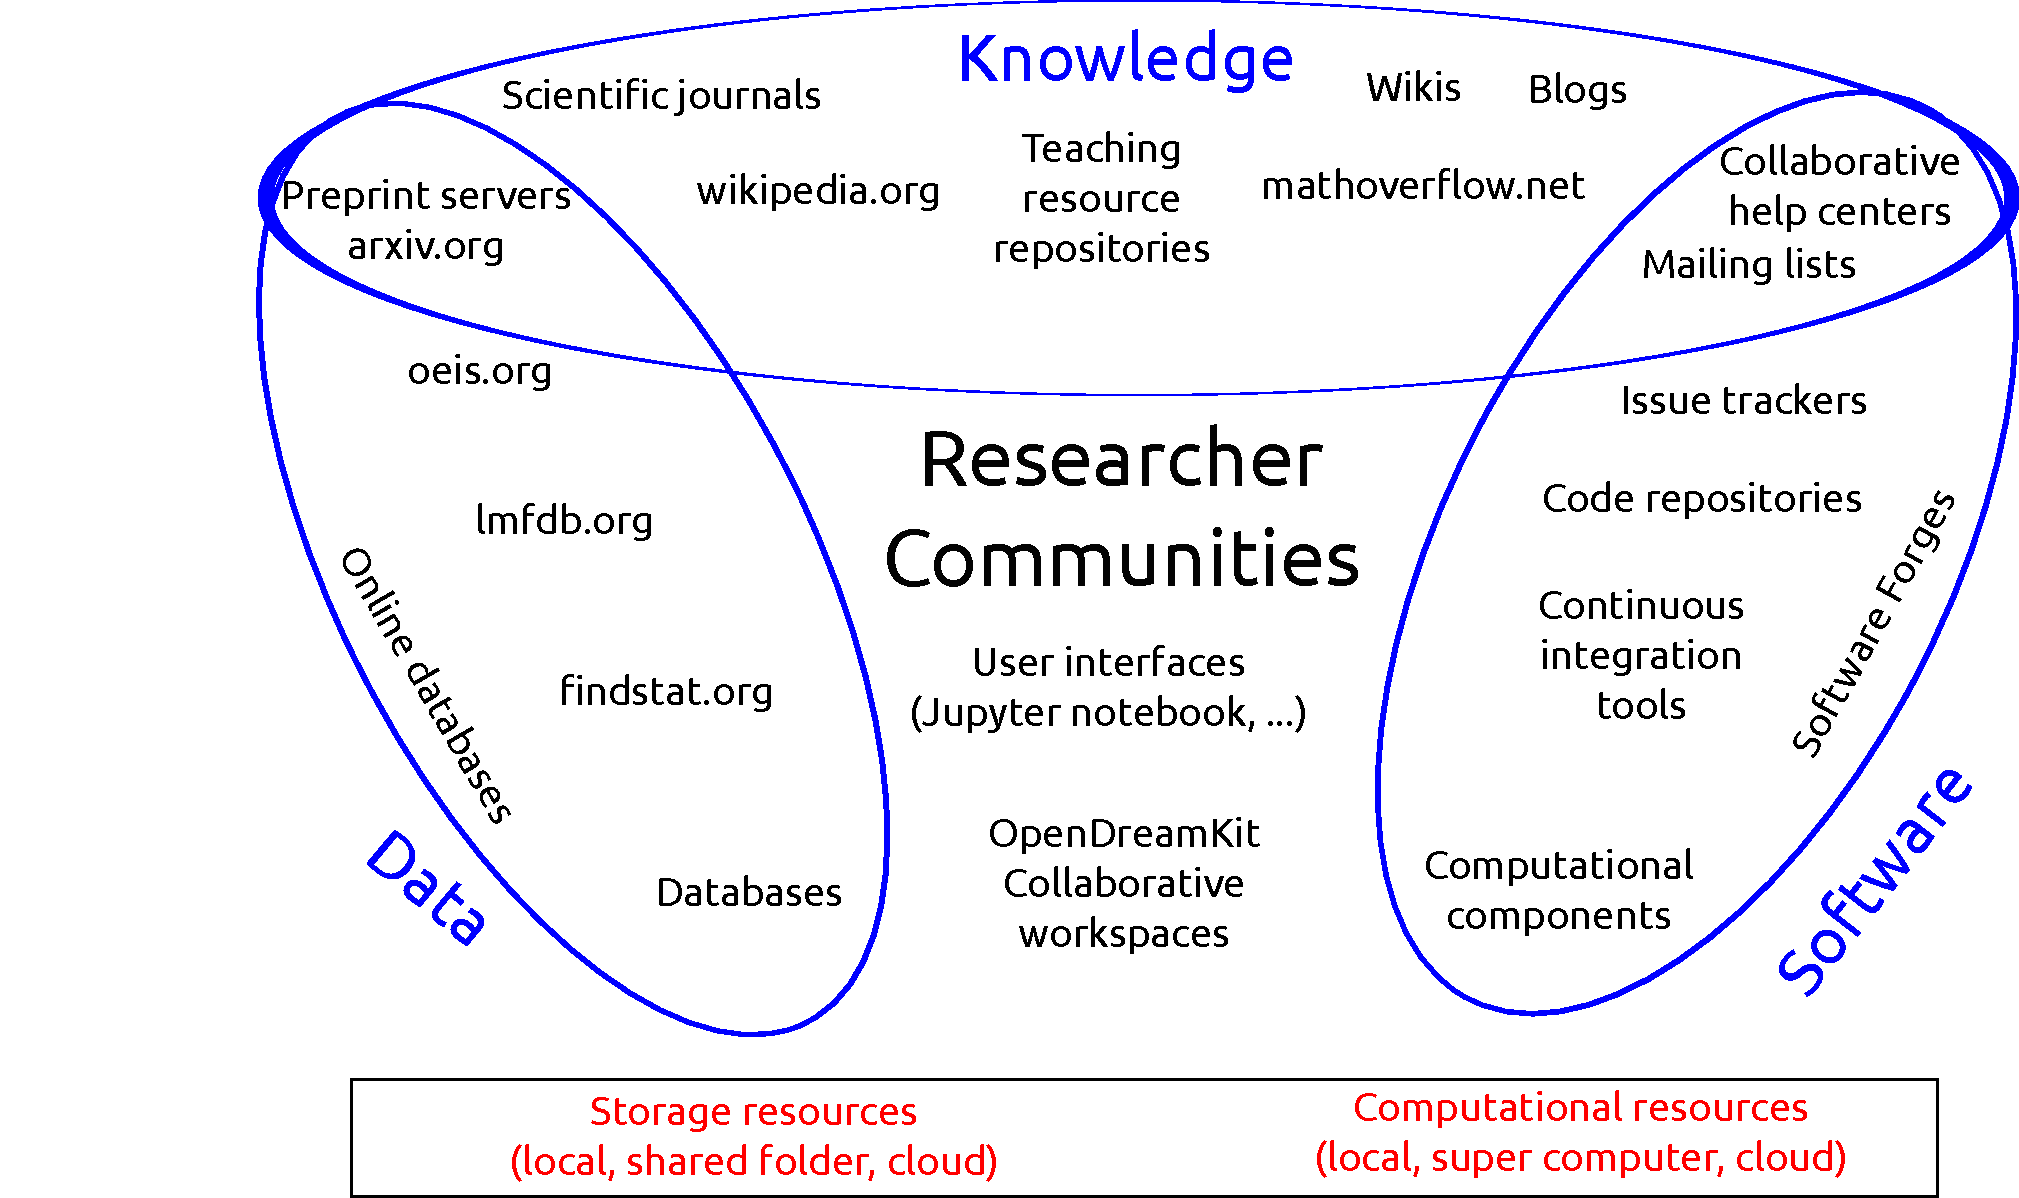
\includegraphics[width=\textwidth]{Pictures/TheBigPicture.pdf}}
  \caption{Virtual Research Environments for research in pure
    mathematics and applications.}
  \label{fig:thebigpicture}
\end{figure}

\begin{center}
\begin{boxedminipage}{.95\textwidth}\em 
Today's research is transformed by the Internet and the availability of vast amounts of
research data on the Internet in virtual research environments. Arguably, Mathematics is
the only science that has not yet benefitted greatly from the systematic interchange of
data. At the same time, mathematics has a richer notion of data than other disciplines.
Indeed, "mathematical data" consists of three kinds of objects:
\begin{compactitem}
\item $\mathcal{D}$: proper (numeric/symbolic) data
\item $\mathcal{K}$: the knowledge about the mathematical objects given as statements
  (definitions, theorems or proofs; either formal or rigorously informal)
\item $\mathcal{S}$ : software that computes (with) the mathematical objects
\end{compactitem}

All three kinds of ``data'' are equally important for mathematics and are tightly
interlinked:
\begin{compactitem}
\item $\mathcal{D}$ serves as examples for $\mathcal{K}$ or as counterexamples for
  conjectures in $\mathcal{K}$;
\item $\mathcal{S}$ computes $\mathcal{D}$ and establishes properties of $\mathcal{D}$
  (given as $\mathcal{K}$);
\item $\mathcal{D}$ tests $\mathcal{S}$, $\mathcal{S}$ is verified with respect to
  $\mathcal{K}$;
\item theorems and proofs in $\mathcal{K}$ induce and justify algorithms for
  $\mathcal{S}$;
\item $\mathcal{D}$ induces conjectures and guides proofs in $\mathcal{K}$.
\end{compactitem}
\end{boxedminipage}
\end{center}
Figure~\ref{fig:thebigpicture} instantiates this situation with respect to the
$\mathcal{DKS}$-resources that are already in use in Mathematics. We name just a few
paradigmatic systems that are relevant in the scope of the \TheProject project: 
\begin{enumerate}
\item \textbf{Data Repositories/Communities}: Many communities have been collecting and
  sharing data about the objects they study: e.g.
  \begin{compactenum}[a.]
  \item The \emph{Open Encyclopedia of Integer Sequences} [\url{http://oeis.org}] has
    collected sequences of integers for half a century, it now contains publications
    about, relations between, programs for, and data on ca. 250.000 sequences and is
    steadily growing
  \item The \emph{database of L-Functions, Modular Forms, and
    related objects} (LMFDB) is an extensive database of mathematical objects
      arising in Number Theory.  The associated website aims to become
      a modern handbook including tables, formulas, links, and references,
      to these objects, including specific L-functions and their sources.
  \item \TOWRITE{Viviane}{findstat}
  \end{compactenum}
\item \textbf{Knowledge Sources and Repositories} There are many ways to represent
  mathematical knowledge and involve computers. Systems and resources range from
  relatively traditional pre-publication systems like
  \begin{compactenum}[a.]
  \item the \emph{Cornell EPrint archive} [\url{http://arxiv.org}] has over 1 million
    {\LaTeX}-based pre-prints of which ca 10-15\% are on mathematics and bordering areas.
  \item via community-driven Q/A sites like [\url{http://mathoverflow.net}] with almost 40
    thousand questions answered  
  \item to mathematical encyclopedias like [\url{http//planetmath.org}], which as a Web2.0
    site predates Wikipedia, 
  \item the LMFDB website [\url{http://www.lmfdb.org}]  which includes novel ways to present this data, following a principle called \emph{transclusion}, 
  and in the extreme to 
  \item formalizations of mathematical knowledge, e.g. in theorem prover libraries like
    Mizar [\url{http://mizar.org}], which has formalized 50 thousand relatively elementary
    theorems in 40 years or the formalizations of the Feit-Thomson Theorem or the Kepler
    Conjecture.
  \end{compactenum}
\item \textbf{Mathematical Software Development and Systems}
  \begin{compactenum}[a.]
  \item \TODO{Please add three interestingly different paradigmatic software systems here}
  \end{compactenum}
\end{enumerate}

 \TheProject aims to create a framework to make the
systems interoperable and synergistic and to give working mathematicians full access to
the potential spanned by already-existing systems. Essentially every node in
Figure~\ref{fig:thebigpicture} represents a user community, so \TheProject is at its heart
a project that also combines researchers and communities.


\TODO{NT: the purpose of Figure~\ref{fig:thebigpicture} is to give a quick
  sense of what Virtual Research Environments can be in our context,
  and a ``big picture'' for the project. A graphic artist friend of
  mine is going to help me improve it. I have collected here some material for her.\\\\
  \textbf{\Large What we would like the ``big picture'' in
    Figure~\ref{fig:thebigpicture} to highlight:}
  \begin{description}
  \item[This is a human centered project:] At the core: researchers and communities
    thereof.
  \item[The three types of information:]
    Software, Knowledge, Data (currently in blue)\\
    How they interact:
    \begin{itemize}
    \item Knowledge help structure data and software (e.g. through ontologies)
    \item Software produce data
    \item Data is used by researchers to build knowledge
    \end{itemize}
  \item[Physical resources:]
    (currently in red)
  \item[Virtual Research Environments]\ 
    \begin{itemize}
    \item Researchers in Math have a long tradition of collaborating
      on Software, Knowledge, and, up to some point, Data
    \item For this they use a variety of collaborative tools which
      form a loosely knit Virtual Research Environment.
    \item \textbf{Aim 2}: make it easy for subcommunities of
      researchers to setup custom collaborative work spaces / Virtual
      Research Environments tailored to their needs, by combining:
      \begin{itemize}
      \item Computational resources
      \item Storage resources
      \item Computational software components
      \item Databases
      \item User interfaces
      \item Wikis-Knowledge bases (true for findstat, LMFDB): quicker
        cycle for consolidation of information spread over
        papers/brains
      \end{itemize}
      Such VRE shall help them:
      \begin{itemize}
      \item collaboratively develop software (e.g. specialized
        libraries), data and knowledge (e.g. articles) for their
        research projects.
      \item contribute back this information to the larger community
        whenever relevant.
      \end{itemize}
    \end{itemize}
  \item[Processes:]\ \\
    It would be interesting to depict the following processes. They
    are indeed about collaboration and sharing (and quality control),
    that is what \textbf{Aim 1} is to promote.
    \begin{description}
    \item[Software development]\ 
      \begin{itemize}
      \item \emph{bug reports} and \emph{enhancement requests} emerge
        from the community, typically through collaborative help
        centers, and are posted on issue trackers.
      \item \emph{Design discussions} occur on mailing lists and issue
        trackers.
      \item Researchers \emph{submit code} to the code repositories.
      \item \emph{Quality control}: the code is reviewed and
        tested by continuous integration tools.
      \item Finally the code \emph{integrated} within computational
        components, and used by the community.
      \end{itemize}
      Researchers (as well as other users: teachers, engineers, ...)
      interact at each step of the process.
    \item[Scientific publication]\ 
      \begin{itemize}
      \item researchers submit articles to journals and post them on
        preprint servers;
      \item the articles get reviewed by other researchers;
      \item finally they are distributed back to the community
      \end{itemize}
    \end{description}
  \end{description}
  %
  Improvements to implement:
  \begin{itemize}
  \item the findstat link does not work for me, kerning looks
    extremely weird -- POD
  \item LMFDB, OEIS, and findstat have a strong knowledge component as
    well, with knowls and wikis, references, ...
  \item arxiv is not far from a database of knowledge
  \end{itemize}
  %
  \textbf{\Large A collection of links that might give some idea of
    the look and feel of our universe:}
  \begin{description}
  \item[Examples of (computational) components:]\ 
    \begin{itemize}
    \item IPython: \url{http://ipython.org/}
    \item GAP: \url{http://www.gap-system.org/}
    \item Singular: \url{http://www.singular.uni-kl.de/}
    \item Sage: \url{http://sagemath.org/}
    \item \PariGP: \url{http://pari.math.u-bordeaux.fr/}
    \item Linbox: \url{http://www.linalg.org/}
    \end{itemize}
  \item[Examples of online collaborative tools]\ 
    \begin{itemize}
    \item Issue tracker: \url{http://trac.sagemath.org/timeline/}
    \item Code repository: \url{https://github.com/}
    \item Collaborative help center: \url{http://ask.sagemath.org/}
    \item Collaborative math site: \url{http://mathoverflow.net/}
    \end{itemize}
  \item[Examples of online databases]\ 
    \begin{itemize}
    \item Online databases: \url{http://oeis.org/?language=french}
    \item LMFDB: \url{http://www.lmfdb.org/EllipticCurve/Q/14.a3}
    \item Findstat: \url{http://www.findstat.org/}
    \end{itemize}
  \item[Example of graphical material]\ 
    \begin{itemize}
    \item \url{http://boxen.math.washington.edu/home/nthiery/main2014.pdf}
    \end{itemize}
  \end{description}
}

\clearpage

\subsubsection{Importance of experimental tools in pure mathematics
  and applications}

From their early days, computers have been used in pure mathematics,
either to prove theorems (e.g. the four color theorem) or, like the
telescope for astronomers, to explore new theories. By now the
experimental method, based on exact computer aided calculations, has
now been added to the standard toolbox of the pure mathematician, and
its usage has grown to the point that certain areas of mathematics now
completely depend on it.

Experiments lead to new conjectures which may have a deep impact on
the future development of mathematics. An outstanding example is the
Birch and Swinnerton-Dyer conjecture which is one of the Clay
Millenium Problems.  Databases relying on computer calculations such
as the Small Groups Library or the Modular Atlas in group and
representation theory provide indispensable tools for researchers. A
constructive way of understanding proofs of deep theorems yields
algorithmic tools to deal with highly abstract concepts. These tools
make the concepts available to a broader class of researchers, with
many potential applications. A prominent example from algebraic
geometry is the desingularization theorem of Hironaka, for which
Hironaka won the Fields Medal, and its algorithmization by Villamayor.

Spectacular theoretical breakthroughs such as the recent complete
resolution of Serre's conjectures, directly inspired by Wiles' proof
of Fermat's last theorem, are based on interdisciplinary approaches.
% Serre's conjecture was in fact proved completely within the last 10
% years, Serre is probably famous enough in Europe (?), and that work
% really is a *direct* extension of work of Wiles; at the same time, the
% conjecture of Serre and much work on it were directly inspired by big
% numerical computations (e.g., by Mestre).
Current developments on the algorithmic side allow one to conquer
cross-connections between different areas of mathematics also
computationally and, thus, to arrive at cutting-edge applications
which previously were inconceivable.

% Computational maths is interdisciplinary by nature

The field of computational mathematics allows us to compute in and
with a multitude of mathematical structures. It is interdisciplinary
in nature, with links to quite a number of areas in mathematics, with
applications in mathematics and other branches of science and
engineering, and with constantly new and often surprising
developments. Quite a number of these developments, in fact the
creation of whole subareas of the field, have been initiated by
European researchers who made crucial contributions at all
levels. These include the design of fundamental algorithms, the
development of major computer algebra systems (\TODO{this is a bit
  redundant with below}), applications of the computational methods in
various fields, and the creation of widely used databases.

Particularly fruitful interactions unfold between computer algebra and
algebraic geometry, number theory, combinatorics and group theory. Algebraic algorithms
open up new ways of accessing subareas of these key disciplines of
mathematics, and they are fundamental to practical applications of the
disciplines. Conversely, challenges arising in algebraic geometry, number
theory, combinatorics and group theory quite often lead to algorithmic breakthroughs
which, in turn, open the door for new theoretical and practical applications
of computer algebra.

\subsubsection{A long track of collaboration on software, data, knowledge}

Supporting the experimental method requires spending major efforts
on software development. As the sophistication of the required
computations increased, supported by the boom of the available
computational power, it became vital to share those efforts at the
scale of large research communities. European mathematicians have been
pioneers and have grown a steady tradition of collaborative open
source software development, with specialized systems like \GAP,
\Singular, or \PariGP playing a major role for decades.

The next scale was reached in the last decade with the advent of the
general purpose mathematical system \Sage which proved the viability
and sustainability of the ``developed by users for users'' development
model at the international level.

\TODO{This is somewhat redundant with the language in
  Objective~\ref{objective:sustainable}; see where this belongs best
  to.}

\TODO{Develop}%
Similarly, mathematicians have been building and sharing databases for
a long while; the needs for such is growing tremendously, and the
process needs to be streamlined.

\TODO{Develop}%
Mathematicians have a strong tradition of sharing knowledge openly
(arxiv, Wikipedia, ...).

% Comment by William:
% > Regarding "Mathematicians have a strong tradition of sharing knowledge
% > openly", I think one reason for this is that the landscape of math
% > research is arguably *dramatically* larger than the research landscape
% > in any other field.  As a result, mathematicians find themselves in a
% > situation where collaboration is far more rewarding and productive
% > than competition, which results in a basic culture of sharing.  In
% > sharp contrast, in areas like drug discover or physics (or perhaps
% > even more intensely, in business!), being extremely competitive and
% > secretive is frequently the best strategy.  It is thus no surprise to
% > us that mathematicians are leading the way in developing tools for
% > collaboration and sharing.      Of course, many people outside of
% > mathematics simply don't know that there is anything to mathematics
% > "beyond calculus", so they don't realize how broad our research
% > landscape is.
% > 
% > I remember a professor in chemistry or physics coming to Sage Days 7
% > at IPAM (UCLA), and remarking that he was very surprised Sage was
% > coming from "number theorists", rather than computer science (say).  I
% > would imagine that computer science is also very competitive, since
% > it's a well-funded area with many people, but compared to mathematics
% > it's basically like one relatively small research area (within
% > combinatorics...).

\subsubsection{Early VRE's}

\TODO{Motivate the relevance of VRE's, in particular by the success of
  \SMC or \Simulagora. Mention as well \LMFDB.}

\TODO{Highlight some other deployed VRE's that would benefit to the
  sorts of improvements you suggest.  You could include Wakari.io and
  also the tmpnb thing in Nature magazine:
  http://www.nature.com/news/ipython-interactive-demo-7.21492}

\subsubsection{Key concept: bringing communities together toward a VRE kit}

\TODO{Focus on VRE kit and building blocks}

\TODO{Why this focus? variability of needs, sustainability, ...}

\TODO{Bringing communities together}

\subsubsection{Linked research and innovation activities}

\eucommentary{Describe any national or international research and
  innovation activities which will be linked with the project,
  especially where the outputs from these will feed into the project;}

\TODO{For each item below, write a paragraph describing the project
  and one describing how it connects with this proposal}

\paragraph{DFG Priority Project SPP 1489}
\url{computeralgebra.de}

The SPP1489 ``Algorithmic and Experimental Methods in Algebra, Geometry, and
Number Theory'' is a nationwide Priority Project of the German Research Council DFG  
which commenced in July  2010 and will end in June 2016. The focus of the programme 
is on the interactions between computer algebra and algebraic geometry, number theory, 
and group theory. It combines expertise at all levels of research in computer algebra, 
be it the design of algorithms, the implementation of algorithms, the application
of algorithms, or the creation of mathematical databases. The goal of SPP1489 is to 
considerably further the algorithmic and experimental methods in the afore mentioned
disciplines, to combine the different methods across boundaries between the disciplines, 
and to apply them to central questions in theory and praxis. A fundamental concern of the
programme is the further development of open source
computer algebra systems with origins in Germany, which in
the framework of different projects will be cross-linked on
different levels. Of particular interest are interactions with application areas inside
and outside of mathematics such as system- and control theory, coding
theory, cryptography, CAD, algebraic combinatorics, and algebraic
statistics as well as hybrid methods which combine numerical and
symbolic approaches. 

The work in the SPP1489 has established effective communication channels between 
the core developers of different computer algebra systems. It is a showcase project
for several objectives of this proposal (such as community building and
fostering a sustainable ecosystem of interoperable open source components). 
The experience made in parallelizing mathematical software will be crucial for
Work package WP5.


\paragraph{IPython/Jupyter grant from the Alfred P. Sloan foundation}
\url{http://ipython.org/sloan-grant.html}

\TOWRITE{IPython}{Proofread description of the Sloan grant and link to this project}

The IPython project received a \$1.15M grant from the Alfred P. Sloan%$
foundation that is supporting IPython development for two years
(1/1/2013-12/31/2014), in particular at the University of California,
Berkeley and California Polytechnic State University, San Luis Obispo.
This grant enabled the project to focus on developing the IPython
Notebook as a general tool for scientific and technical computing that
is open, collaborative and reproducible. This goes a long way toward
Aim \TODO{... and ...} of \TheProject, especially given the current
rapid evolution of IPython toward its language agnostic avatar
Jupyter.

\TheProject will build on the outcome of the Sloan grant, and further
develop the critical IPython/Jupyter component in close collaboration
with the IPython/Jupyter team. In particular, we plan to hire some of
the European developers that are currently funded by the Sloan grant
to work in California and wish to later return to Europe.

\paragraph{NSF SI2-SSE OCI-1147247}

%\SageCombinat is a subproject of \Sage whose mission is "to improve
%\Sage as an extensible toolbox for computer exploration in (algebraic)
%combinatorics, and foster code sharing between researchers in this
%area".

The OCI-1147247 Collaborative Research grant ``Sage-Combinat:
Developing and Sharing Open Source Software for Algebraic
Combinatorics'' is a project funded by the National Science Foundation
from June 2012 to May 2015. The grant supports the development of
\SageCombinat, on the USA side, and in areas relevant to the ongoing
research of the participants (symmetric functions, Macdonald
polynomials for arbitrary Cartan types, crystals, rigged
configurations and combinatorial R-matrices, affine Weyl groups and
Hecke algebras, cluster algebras, posets, ...), together with relevant
underlying infrastructure. The grant funds a yearly Sage Days
workshop, and cofunded two others at ICERM and Orsay respectively. The
grant also funds a dedicated software development and computation
server for \SageCombinat, hosted in the \Sage computation farm in
Seattle. Emphasis is placed on the development of thematic tutorials
that make the code accessible to new users. The grant also funds
graduate student RA support, curriculum development, and other
mentoring.

Two of the proposers, Stein and Thiéry, are respectively PI and
foreign senior participant to this NSF grant. It funded, through them,
some of the development of \SMC as well as of the category framework
in \Sage; both are key assets for this proposal. The workshop and
outreach actions pursued by this NSF grant have proven to be potent
tools for connecting researchers and recruiting users and
developers. One of the role of this proposal is to support similar
community building in Europe.

\paragraph{HPAC grant from the A.N.R.}

The French national research agency ANR has funded a 4 years project
on High Performance Algebraic Computing (HPAC) focused on the
development of parallel exact linear algebra. The consortium gathers
research groups from LIP6 (Paris 6), LIRMM (Montpellier), LIP (Lyon)
and LIG and LJK (Grenoble). The main goals of the project is to first
develop high performance exact linear algebra kernels with dedicated
parallel runtime, propose a domain specific language for the
parallelization of exact linear algebra libraries and their
composition, invent new algorithmic solutions for large scale
parallelizations. The output of the project is then twofolds: new
computational challenges arising in algebraic cryptanalysis will be
addressed, and the open-source libraries maintained by each group will
not only integrate these advances, but will expose them in a close
integration to high level computer algebra softwares. In this process,
\Sage will start benefitting from the new shared-memory parallel code
of \Linbox for the linear algebra over a finite field.  The scope of
this project is mostly focused on shared memory parallelism (except
for some challenge computations). Addressing distributed and
heterogeneous infrastructures is the next step after this project,
that is be addressed in work-package 5 of the this proposal.


\paragraph{RADIANT Grant from EU FP7-HEALTH (ref 305636)}
\url{http://radiant-project.eu/}

This EU funded proposal focuses on making available computational and
mathematical models to the computational biology communities as
rapidly as they are developed with a particular focus on high
throughput sequencing techniques. The rapid development of sensorics
technology in the biological sciences results in mathematical
challenges in the data analysis. To address these challenges in a
timely manner collaborative frameworks for mathematical and
computational modelling are required. \TheProject provides the
framework for pipeline delivery of methodologies to end users through
approachable IPython/Jupyter notebooks.

% for an example see: http://nbviewer.ipython.org/github/SheffieldML/notebook/blob/master/compbio/index.ipynb

\paragraph{Logilab: simulagora, cubicweb, ...}

\TOWRITE{Logilab}{One paragraph description of simulagora, cubicweb, ...}
\TOWRITE{Logilab}{How does it relate to this project}

\paragraph{Sage Math Cloud} \url{https://cloud.sagemath.com/}

\SMC provides a collaborative online environment for students,
teachers and researchers to interact with \Sage and with each
other. It has \Sage and \IPython worksheets, powerful \LATEX editing
features and a full \Linux computer, all accessible from a standard
web browser. Its main design feature is to enable and promote
collaboration between groups of users. It is for example a natural
place to host a course, allowing teachers to collaborate with their
students using modern tools like \Sage and \LATEX, with facilities for
real-time communication through chat, video, and shared editing of
documents, programs and worksheets; course material can be provided as
worksheets, assignments can be distributed, collected, and returned as
well. Launched in 2013, \SMC presently hosts over 100,000 projects and
10,000 weekly active users. This fast adoption by a wide variety of
users demonstrates the relevance and the long term impact this kind of
collaborative environments can have.

Technically speaking, \SMC is a specific open-source cloud-based
Virtual Research and Teaching Environment for mathematics developed
since 2013 under the lead of William Stein, with funding from the NSF,
and Google's Education Grant program. It's currently deployed at the
University of Washington at Seattle, with a business plan in the work
for commercial support for massive on line courses, subsidizing a free
service for all other academic usage and some further \Sage
development.

In comparison \TheProject focuses on open source building blocks and
architecture to easily setup and deploy custom Virtual Research
Environments. On the one hand, \SMC will serve as prototype for
\TheProject, paving the way and showcasing important features from the
users perspective. On the other hand, basically each and every task
undertaken in \TheProject will benefit back \SMC.

\paragraph{FLINT grant?}

\paragraph{LMFDB grant}\url{http://www2.warwick.ac.uk/fac/sci/maths/people/staff/john_cremona/lmf}

The L-functions and Modular Forms Database (LMFDB) project originated
at a meeting at The American Institute for Mathematics (AIM) in 2007.
L-functions are ubiquitous in number theory, and have applications to
mathematical physics and cryptography. The simplest example of an
L-functions is the Riemann zeta function. Two of the seven Clay
Mathematics Million Dollar Millennium Problems deal with properties of
these functions, namely the Riemann Hypothesis and the Birch and
Swinnerton-Dyer Conjecture, that were conjectured following
computational exploration.  As well as providing a central repository
of data as a resource for researchers, through its website
\url{www.lmfdb.org}, the LMFDB provides a modern handbook, including
tables, formulas, links and references, concerning particular specific
L-functions and their sources.  Between 2008 and 2012 the LMFDB was
funded through a US National Science Foundation (NSF) Focussed
Research Grant (FRG) of around \$1M.  Since 2013, the funding of the%$
LMFDB has passed to Europe through a six year £2.2M Programme Grant
(grant reference EP/K034383/1) from the UK Engineering and Physical
Sciences Research Council (EPSRC), held at the universities of Warwick
and Bristol, with Professor John Cremona (Warwick) as its Principal
Investigator.  This grant supports six three-year postdoctoral
research fellows, mathematical researchers who work on the
mathematical aspects of the project full-time, biannual workshops,
equipment and a portion of the investigators' own time.

Almost all contributors to the LMFDB project, including those directly
supported by the EPSRC grant and the larger world-wide team of 30-50
contributors of data and code, are pure mathematicians.  Most of these
have good computational skills, but are not professional programmers
or software developers.  The LMFDB has a great need to broaden the
support it can call upon from software developers, to enhance the
project in several ways, including the computation of number-theoretic
data but more specifically in supporting the database management and
website user interface, in order to make the data more accessible and
useful to others.  The codebase of the LMFDB project is entirely open
source and hosted at GitHub \url[https://github.com/LMFDB/lmfdb], written
in python with specialist modules such as flask and pymongo to manage
the website and database interface, and \Sage\ for higher-level
mathematical computations.  It also implements ``Knowls'', a very fruitful method of presenting mathematical knowledge.

The LMFDB project would therefore benefit
greatly from collaboration with \TheProject as it would connect the
project with a pool of experts.  Joint workshops between the LMFDB and
\TheProject will stimulate and develop such collaboration: the LMFDB
places great importance on its workshops, which are small gatherings
of around 30 invited participants who work throughout one week on
certain specific aspects of the project, coming together in plenary
sessions to make decisions, plan and collectively approve of proposed
developments.  As a leading example of the use of databases in
mathematical research, the LMFDB will provide \TheProject\ with a real
large-scale prototype around which to develop new ideas about the
design and implementation of such databases and their associated
software.  The feasibility of such collaboration was successfully
tried at a workshop at the ICMS in Edinburgh in January 2013 on
``Online databases: from L-functions to combinatorics'', sponsored by
the NSF, AIM and the ICMS.

\paragraph{Edith Elkind's ERC Starter Grant} awarded in 2014, titled
``Algorithms for Making Complex Decisions on Structured Domains'', 
will develop theoretic tools for analysing and improving situations
arising in collaborative environments. 
It can be viewed as a interdisciplinary project, bringing together methods from
computer science, game theory, and economics and political science
to quantify complex behaviour of social interactions.

\TheProject\ appears to be a natural
testing ground and a potential virtual laboratory for developing and testing
ideas and tools developed, within the framework of the ERC Grant, 
on in a ``real life'' situation, and the collaboration
will be mutually beneficial for both projects.

 
\paragraph{Ursula Martin's EPSRC funded project}
``MathSoMac: The Social Machine of Mathematics'' (EP/K040251/2) brings rigorous methods from social
sciences into studying of the crowdsourcing, e.g. large-scale online
collaboration, phenomenon in mathematical sciences. 

\TheProject\ and VREs in general are natural objects to investigate for the
latter project, and conclusions drawn would lead to better understanding
of the ways VREs function. This has important potential benefits for \TheProject, and
vice versa. 



\paragraph{Findstat?}

\paragraph{KWARC group}

\paragraph{HPCGAP}

\paragraph{CoDiMa} is a new EPSRC funded Collaborative Computational Project 
in the area of {\em Co}mputational {\em Di}screte {\em Ma}thematics (EP/M022641/1).
It will begin in 2015 and will be aimed at \GAP and \Sage community-building 
activities in the UK, involving a programme of short research visits, workshops 
and training events. Through CoDiMa, we will have an excellent opportunity to
interact with UK user and developer communities of \GAP and \Sage in order to
to collect feedback about their requirements and to inform them about \TheProject 
outcomes.
%%% Local Variables: 
%%% mode: latex
%%% TeX-master: "proposal"
%%% End: 

%  LocalWords:  eucommentary programme authorisation includegraphics textwidth textbf
%  LocalWords:  thebigpicture subcommunities findstat emph emph knowls IPython Linbox
%  LocalWords:  clearpage subsubsection Swinnerton-Dyer Millenium desingularization Serre
%  LocalWords:  Hironaka algorithmization Villamayor Serre's Mestre Simulagora Wakari.io
%  LocalWords:  tmpnb computeralgebra.de Jupyter TOWRITE SageCombinat Sage-Combinat Weyl
%  LocalWords:  Macdonald Cartan cofunded Thiéry sensorics modelling Logilab cubicweb
%  LocalWords:  github pymongo boxedminipage compactitem mathcal compactenum EPrint
%  LocalWords:  Feit-Thomson


\draftpage
% ---------------------------------------------------------------------------
%  Section 1.4: Ambition
% ---------------------------------------------------------------------------
\subsection{Ambition}



\eucommentary{1-2 pages}

\eucommentary{-- Describe the advance your proposal would provide beyond the
state-of-the-art, and the extent the proposed work is ambitious. Your answer
could refer to the ground-breaking nature of the objectives, concepts
involved, issues and problems to be addressed, and approaches and methods to be used.\\
-- Describe the innovation potential which the proposal represents. Where relevant, refer to
products and services already available, e.g. in existing
e-Infrastructures.}

For most pure mathematicians using computational tools in their
research, the state of the art in the beginning of 2015 is still a collection of
programs each of which must be installed individually on their
desktop or laptop computer, respecting a complicated dependencies graph.
Alternatively software may be installed on a
departmental server or cluster and used via text-based remote
login. The software performs computations (using excellent
implementations of extremely sophisticated algorithms) with inputs and
outputs usually in a bespoke text-based format. 
Multiple computations involved in producing a mathematical
result must be managed by editing, naming and filing multiple scripts
or programs, and there is no automatic support for rerunning
computations to check for human or algorithmic error. The results of
computations are incorporated into publications by cut-and-paste and
collaboration is through exchange of programs and data by email,
shared general-purpose file servers or, rarely, a service such as
GitHub. Such situation creates a serious obstacle to the reproducibility
of computational experiments reported in research publications,
(even by their authors themselves after a duration of time). 
% see e.g. "Case Studies and Challenges in Reproducibility in the 
% Computational Sciences", http://arxiv.org/abs/1408.2123, submitted

There are commercial ``symbolic computation systems'' such as
\Mathematica or \Maple which offer somewhat more modern frameworks, but
they lack the specialised algorithms for research work in fields such
as algebra, number theory or algebraic geometry and are not
well-suited to support them. 
\TODO{This statement needs verification. It's not only the lack of algorithms
in these areas. Moreover, we want to cater for wider areas of mathematics}

The need for a more modern, more productive and less error-prone
environment for this kind of mathematical research computing is widely
acknowledged, but the separate groups developing the systems have
individually, neither the time nor the expertise to develop it. There
have been a number of interesting projects which have explored
different aspects of what is needed, in particular
\SMC (see \ref{linked-projects});
\HPCGAP (\TODO{now listed under St Andrews entry});
\scienceproject (\TODO{now listed under St Andrews entry});
\Sage and \Sage notebooks itself;
Polymath and MathOverflow (see MathSoMac entry in \ref{linked-projects});
and \software{Recomputation.org}.
We will build on the experiences, and where useful, on the software, of all of these.

Our ambitious plan in this project is to learn from, and leapfrog,
these piecemeal developments and provide a toolkit of software and
interfaces, which supports the whole mathematical research process in
a way which is \textbf{modern}, \textbf{seamless},
\textbf{collaborative}, mathematically \textbf{rigourous} and
\textbf{adaptable} to the diverse needs of different mathematical
research areas and of different mathematicians and collaborations.

\TODO{Explain all the highlighted words in the para above}

\TODO{Some examples here -- what will we deliver to individuals; small ``single-problem''
  collaborations; longer-lived data- or algorithm- centred teams;
  massive ``flagship'' projects. Think ``User Stories''. 
  AK: for example, a paragraph below.}
  
These will offer functionality for collaborative computational projects
of all possible scales. An individual researcher would use it for a new
experiment because it will be easier to start it in VRE than to not to;
a small multi-site team would set up a project easily shareable between
current and prospective collaborators and accessible from anywhere in the
world; providers of mathematical databases will be able to find a long-term
solution for offering mathematical data for the community maintaining
high-quality provenance and composability standards; Massive ``flagship''
algorithm-centred projects will increase their productivity from all
collaborative features that may be integrated under a single VRE.

\subsubsection{Challenges specific to  mathematics}

Mathematical research, especially pure mathematics, presents some
unique challenges to the realisation of this ambition.

\TODO{Evidence this in more detail, clean up the language}

\begin{itemize}
\item The community mainly comprises of individuals or \textit{very} small
  groups (say, a PI and a few students), having fewer formal or structured research
  groups such as you might find in an equipment-intensive science. There are 
  certainly examples of large scale collaborations happen (CoFSG, Polymath),
  but these are still driven by individuals, not by formal structures or funding bodies.
\item Many exemplars of top quality research have little or no formal research
  funding. In case they need computational resources, these are limited to what 
  is already available nearby, such as personal laptops or departmental clusters.
\item Many mathematical computations are highly complex and irregular. Thus,
  traditional HPC paradigms coming from numerical simulations and linear algebra do not apply.
\item Mathematical notations have been refined over many centuries to be
  used by humans with pen, paper and blackboard. Even such simple
  problems as selecting a sub-expression are hard to handle well on a
  computer. For instance $a+c$ is naturally seen as a subexpression of
  $a+b+c$ by a human.
\item The mathematical correctness of widely used algorithms hinges on
  quite complex chains of reasoning. Subtle coding errors may easily
  produce plausible, but wrong, answers.

\item Mathematical data differ in several ways from typical
  scientific data
  \begin{itemize}
  \item More often rather than not, data is the result of a computation (and
    not a measurement of the real world). The role of databases is thus primarily
    to store results for later search and reuse (persistent caching). 
    Because of this, many issues (semantics, ontologies,
    reproducibility) are to be treated upstream at the level of
    software rather than data.
  \item Extreme reification in mathematics makes classical ontologies
    techniques (such as e.g. RDF) impractical. \TODO{Someone explain this}
  \item Data are highly interlinked and based on a hierarchy of mathematical objects,
  which, in their turn, may have more than one (interchangeable) definition.
  \end{itemize}
\end{itemize}

\subsubsection{Challenges of a community built around multiple
  existing software projects}

Another source of unique challenges for this project is the need to
interact with several large and diverse ecosystems of software
developers. For instance the \GAP package development community, the
\Sage development community, the wider Python community, the developers
of key open-source libraries on which we rely and so on.

These communities exist in a delicate balance between collaboration
and competition. For instance the \scienceproject and \Sage were
simultaneously exploring two different approaches to linking
open-source mathematical software. Many technical developments (better
IO handling in \GAP, for instance) could usefully be shared, and at
the end of the day we all want to do better mathematics, but a certain
degree of competition is both natural and healthy.

In this project we need to build a sustainable ``meta-ecosystem'' in
which systems may compete to have the best designs or algorithms, but
all agree to cooperate on interfaces, bug reporting, testing, etc. to
keep the final user experience seamless and reliable.

\TODO{Promoting collaboration over competition between communities.}

\TODO{Describe innovation potential}
%%% Local Variables:
%%% mode: latex
%%% TeX-master: "proposal"
%%% End:

%  LocalWords:  eucommentary textsuperscript textregistered textsuperscript specialised
%  LocalWords:  textregistered recomputation textbf textbf rigourous centred flagshsip
%  LocalWords:  subsubsection realisation textit


\draftpage
% ---------------------------------------------------------------------------
%  Section 2: Impact
% ---------------------------------------------------------------------------
% ---------------------------------------------------------------------------
%  Section 2: Impact
% ---------------------------------------------------------------------------

\section{Impact}
\label{sec:impact}

\TOWRITE{Simula}{Hans Petter and Valeriya will make a second iteration on the impact section for Friday}

\subsection{Expected Impacts}

\eucommentary{Please be specific, and provide only information that applies
to the proposal and its objectives. Wherever possible, use quantified
indicators and targets.\\
Describe how your project will contribute to:\\
-- the expected impacts set out in the work programme, under the relevant topic
(including key performance indicators/metrics for monitoring results and impacts);\\
-- improving innovation capacity and the integration of new knowledge
(strengthening the competitiveness and growth of companies by developing
innovations meeting the needs of European and global markets; and, where
relevant, by delivering such innovations to the markets;\\
-- any other environmental and socially important impacts (if not already
covered above).\\
Describe any barriers/obstacles, and any framework conditions (such as
regulation and standards), that may determine whether and to what extent
the expected impacts will be achieved. (This should not include any risk
factors concerning implementation, as covered in section 3.2.)}

\subsubsection{Impacts as listed in the work programme}

The following table shows how \TheProject  addresses the specific impacts
listed in the work programme.

%\TOWRITE{NT}{Double check the table below: margins + where the checks
%  are in the measures to maximize impact}
\def\tmc#1{\hline\multicolumn{2}{|m{.94\textwidth}|}{\textbf{#1}}\\\hline}
\tablehead{}
\begin{supertabular}{|m{.47\textwidth}m{.47\textwidth}|}\hline
  \tmc{More effective collaborations between researchers}

  \TheProject will strengthen collaborations between European scientific community in
  different branches of mathematics, through a development of the common e-infrastracture
  by bringing together software and databases previously separated, and build links with
  scientific communities in other disciplines (biology, physics, astronomy) that will use
  this e-infrastructure. The scientific community will considerably increase, by
  integrating new actors both from academic and non academic sector. & Key performance
  indicators :
  \begin{compactenum}
  \item By the end of the project, the scientific community in mathematics using the tool
    will increase by X \%
  \item The scientific community in other disciplines (biology, physics) using the tool
    will increase by X\%
  \item Number of enterprises using the tool will increase by X\%
  \end{compactenum} \\\hline

  \tmc{Higher efficiency and creativity in research, higher productivity of researchers
    thanks to reliable and easy access to discovery, access and re-use of data}

  The development of a new integrated tool, replacing 3
    previously separated tools, a possibility of real time data sharing, data re-use and
    simultaneous working will allow an important gain in time and in efficiency, and, by
    consequence, higher productivity of researchers. Moreover, the exchange of best
    practice (such as regular audit of codes) will have an important impact on the quality
    of the research. Finally, the unique tool will allow considerably reducing the costs
    of further research.

 &

  Key performance indicators :
  \begin{compactenum}
\item The e-infrastructure developed by the end of the project will help reducing time of
  research by X\%\item The productivity of researchers will increase by X\%\item Thank to
  best practice exchange, the quality of research will considerably increase and number of
  errors will be reduced\item Better traceability of research \item Costs for research
  considerably reduced
\end{compactenum}
\\\hline
\tmc{Accelerated innovation in research via
an integrated access to digital research resources, tools and services
across disciplines and user communities}

An integrated access to digital research
resources and tools that \TheProject will provide will clearly help
accelerating innovation in research across disciplines and communities.

The integrated tool will meet the needs and help overcoming the
obstacles that are common to several disciplines impacted by the
project, and both to academic and non-academic research. Industrial
actors, actively involved into the project will directly benefit from
the project results. &

Key performance indicators :

\begin{compactenum}
\item Emergence of new, improved research methods in several disciplines
using the tool\item Resolution of series of problems proper to
industrial actors in several disciplines
\end{compactenum}
\\\hline

\tmc{Researchers able to process structured and qualitative data in virtual and/or ubiquitous workspaces}

\TheProject will enable researchers to process
different kind of  data thanks to an integrated tool interconnected
with databases. Efficient data storage will allow further exploitation
and  re-use of mathematics data for further calculations and thus make
data processing more efficient.

Le travail sur la sémantique de données est fait plus en amont.
 &
Key performance indicators :

Note E.S. – Nicolas, ici, j'ai du mal, car pas sure si on répond
vraiment à ce critère.\\\hline

\tmc{Increased take-up of collaborative research and data sharing by new disciplines,
  research communities and institutions}

The project will clearly enhance a take-up
of collaborative research and data sharing by and between new
disciplines and research communities. The communities already using the
parts of the tool, will be enlarged, involving more and more industrial
actors and young scientists.

By developing the tool, it will reinforce collaborations between
different branches of mathematics (both pure and applied). Once
developed, the tool will be opened for research in various disciplines,
such as biology, physics, astronomy etc. &
Key performance indicators :

\begin{compactenum}
\item Increased collaborations and data sharing between different communities in
  mathematics
\item Increased collaborations and data sharing between research communities in other
  disciplines
\item Increased number of users, enlarged research communities
\end{compactenum}
\\\hline
\end{supertabular}

\subsubsection{Improving innovation capacity and the integration of new knowledge}


 Innovations developed by \TheProject project will meet the needs of the
following ecosystem participants:

\begin{enumerate}
\item Device / module vendors: hardware manufacturers, equipment
manufacturers of smartphones, tablets, laptops;
\item Network providers: service providers, network infrastructure
vendors (Avaya, Juniper, Extreme, Cisco…)
\item Platform providers
\item Cloud service providers: Software-as-a-Service,
Platform-as-Service, Infrastructure-as-a-Service
\item Systeme integrators: end-to-end integration services and
value-added services (Accenture, HP, IBM…)
\item End users: research communities; IT, healthcare, education and
aeronautics stakeholders
\end{enumerate}
Industrial stakeholders will be directly involved into the project and
the VRE development, so that the tool will be exactly tailored to their
specific needs – that are the same that the scientific community ones.
Moreover, this will allow an early time-to-market and will facilitate
the technology uptake.

In the table below we have specified different market needs, and the
ways the project will address each of them :

Table XX

\begin{flushleft}
\tablehead{}
\begin{supertabular}{|m{.47\textwidth}|m{.47\textwidth}|}
\hline
\centering Needs of markets &
\centering\arraybslash How the project will address these needs\\\hline
Performance gain &
The tool will enable its users to combine functionality from XXX other
mathematical software programs and programming languages

{}-mainstream programming language Python?

{}-which compilers?\\\hline
Infrastructure capacity: newly built infrastructures with fast broadband
connections are well positioned for adoption &
\TheProject will allow different groups of users to work simultaneously, and
thus provide a considerably gain in efficiency.\\\hline
Lower cost of scaling  &
An open source architecture brings affordability: people and
organizations donate towards common goals, and small organizations can
gain access to equipment and research talent typically only afforded by
the largest firms. Resources integration will reduce considerably the
time and the costs of operations.\\\hline
Going beyond limitations of interconnect technology &
An open source architecture brings creativity (=the best minds to solve
a problem)\\\hline
Enabling new applications and features &
Through a series of links that will be created between previously
separated tools, and data interoperability, the VRE will enable new
applications and features\\\hline
Early time-to-market (TTM): companies are looking for solutions that
would improve the speed at which they can procure services to bypass
traditional information technology departments &
The speed of development will improve tremendously thanks to open
source. The implication of industrial stakeholders into the development
will allow to deliver a tool the suits the best to their needs, and
thus speed-up the time to market and technology uptake.\\\hline
Easy-to-use service: first-time experiences is crucial to gain
acceptance &
{}-Design? Ergonomie? Nice multiuser web-based graphical user interface

{}-integration with learning tools? (example : interactive whiteboard)

\TOWRITE{NT}{E.S: Nicolas, il faut réflechir à la façon de rendre l'outil
plus attractif pour la jeune génération (=future génération des
chercheurs), car c'est la génération Y qui va définir des standards
pour la suite  {}- donc  plus d'impact et à plus long terme. Réfléchis
à la possibilité de rendre l'outil accessible sur mobiles, tablettes
etc., mais aussi à la façon ``~intéressante~'' de l'enseigner.}\\\hline
\end{supertabular}
\end{flushleft}

\subsubsection{Other impacts (environmental and socially important impacts)}

\TODO{Neil: Can we not be more ambitious than simply replacing the other alternative? By working in an open way we should be able to achieve much more rapid deployment of ideas (like in the RADIANT project I mentioned above).} 

Here, our mission statement will be the same as for \Sage: to provide
a viable free open source alternative to \Magma, \Maple, \Mathematica
and \Matlab.

To make \TheProject a new reference, it is important to focus on the young
generation, which will be the future users.

Generation Y phenomenon:

\begin{compactenum}
\item generation Y accounts for 30\% of the total projected population
in 2025
\item key influencers to change in workplace habits
\item easy adaptability to technology -{\textgreater} collaborative work
would make them more productive
\item compulsion to check smartphones for emails, texts or social media
updates -{\textgreater} adoption of social networks.
\end{compactenum}
2.1.4. Potential barriers and framework conditions (such as regulation
and standards), that may determine whether and to what extent the
expected impacts will be achieved. (This should not include any risk
factors concerning implementation, as covered in section 3.2.)

The project does not arise any specific regulation issues; in the
unlikely event that new norms would appear during the project,
appropriate measures will be taken by the advisory board following
advice of relevant experts and standards agencies on national and EU
level.

\subsection{Measures to Maximise Impact}

\subsubsection{Dissemination and Exploitation of Results}
\label{subsubsect:dissemination}

\eucommentary{-- Provide a draft 'plan for the dissemination and exploitation
of the project's results'. The plan, which should be proportionate to the
scale of the project, should contain measures to be implemented both during
and after the project.\\
Dissemination and exploitation measures should address the full range
of potential users and uses including research, commercial, investment,
social, environmental, policy making, setting standards, skills and
educational training.\\
The approach to innovation should be as comprehensive as possible,
and must be tailored to the specific technical, market and organisational
issues to be addressed\\
-- Explain how the proposed measures will help to achieve the expected impact of the
project . Provide a draft business plan for financial sustainability as stated in the Part
E of the Specific features for Research Infrastructures of the Horizon 2020 European
Research Infrastructures (including e-Infrastructures) Work Programme 2014-2015.\\
-- Where relevant, include information on how the participants will
manage the research data generated and/or collected during the
project, in particular addressing the following issues:
What types of data will the project generate/collect? What
standards will be used? How will this data be exploited and/or
shared/made accessible for verification and re-use (If data cannot
be made available, explain why)? How will this data be curated and preserved?\\
-- Include information about any open source software used or developed by the
project.\\
You will need an appropriate consortium agreement to manage (amongst other things)
the ownership and access to key knowledge (IPR, data etc.). Where relevant,
these will allow you, collectively and individually, to pursue market opportunities
arising from the project's results.\\
The appropriate structure of the consortium to support exploitation is addressed
in section 3.3. \\
-- Outline the strategy for knowledge management and protection. Include measures to
provide open access (free on-line access, such as the ``green'' or ``gold'' model) to
peer-reviewed scientific publications which might result from the project.\\
Open access publishing (also called 'gold' open access) means that an article is
immediately provided in open access mode by the scientific publisher. The associated costs
are usually shifted away from readers, and instead (for example) to the university or
research institute to which the researcher is affiliated, or to the funding agency supporting
the research.\\
Self-archiving (also called ``green'' open access) means that the published article or the
final peer-reviewed manuscript is archived by the researcher - or a representative - in an
online repository before, after or alongside its publication. Access to this article is often -
but not necessarily - delayed (``embargo period''), as some scientific publishers may wish to
recoup their investment by selling subscriptions and charging pay-per-download/view fees
during an exclusivity period.}

Three types of impact are possible with our dissemination and
communication activities: (1) people or organizations are informed
about \TheProject; (2) people or organizations act and use our conclusions
or results; (3) people or organizations contribute and help to develop
or improve the research infrastructure. The second form of impact
supposes that parties understand the messages. The third form supposes
learning, which is a very high level of impact. In the following table,
we have listed how the proposed measures will help to achieve the
expected impact among our stakeholders and target audiences.

Table X.  Draft 'plan for the dissemination and exploitation of the
project's results'.

\begin{flushleft}
\tablehead{}
\begin{supertabular}{|m{2cm}|m{8cm}|l|l|l|}
\hline
Target users &
Measures during the project &
\multicolumn{3}{m{3.9129999cm}|}{Expected impact}\\\hline
 &
 &
(1) &
(2) &
(3)\\\hline
Scientific community in mathematics

(experienced researchers and PhD students) &
\begin{compactenum}
\item Recruitment for the project of specialists from industrial sector
and PhD students that are already a part of the community ;\item 10
technical workshops organized in the frame of \TheProject,  \item 10
scientific trainings/year,  \item Participation to
international conferences like FPSAC, ISSAC, ... (4), international congress of mathematical
software (1)\item Workshops ``Sage and women'' (1?)\item 10
publications in (social aspects) \item Software demonstration during
the conferences{\textgreater}publication\item 100 PhD students trained
and accessing the infrastructure\item Workshops for PhD students in
Africa
\end{compactenum}
 &
X

X

X

X &
X

X

X

X

X

X

X &
X

X

X

X

X

X\\\hline
Scientific community in other disciplines &
\begin{compactenum}
\item Direct implication of the representatives of those disciplines
into the project;\item Annual participation in Pycon international
conference\item X scientific trainings to other communities; \item News
in Nature and other editions in other disciplines (specify!)\item Up to
X PhD students trained on the tool in biology, physics etc.\item
Workshop ``~sage \& women~'' in USA{\textgreater} pour
IPython
\end{compactenum}
 &
X
 &
X
X
X
X
X
X
 &
X
X
X\\\hline
Policy makers &
Are not directly concerned by the tool, but can be informed via
international conferences and publications &
X &
 &
\\\hline
Industry &
\begin{compactenum}
\item Industrial stakeholders have common needs with academic
researchers. They bring to the project their specific competences and
human resources. They are actively involved into the workshops and
trainings (50\% of audience). The project aims the enlargement of the
community thanks notably to new industrial actors (including in other
disciplines and sectors). They will appropriate the tool by their
direct involvement into the project, by participation to the workshops,
trainings and conferences or by their usual information channels.\item
Annual participation in Pycon international conference\item
Certification by technology clusters
\end{compactenum}
 &
X &
X
X
X
 &
X\\\hline
Standartisation

agencies  &
\begin{compactenum}
\item At the end of the project,~after internal standartisation, the new
norms will be accorded with specialized agencies at national and EU
levels
\end{compactenum}
 &
 &
X &
\\\hline
Students &
\begin{compactenum}
\item 5 MooCs destined to master students.\item The tool will be used
for the elaboration of pedagogical documents, referenced on the
specific website\item The projects results will be integrated into
Master courses, and into teacher training courses
\end{compactenum}
 &
X
X
X
 &
X
X &
\\\hline
Civil society &
\begin{compactenum}
\item Results will be presented on the annual event “Worldwide meetings
of the free software”. This event generally touches upon all free
phenomena in the society, and involved various stakeholders, including
civil society actors.
\end{compactenum}
 &
X &
X &
\\\hline
Public at large &
\begin{compactenum}
\item Series of actions in high schools led by PhD students to raise
awareness of pupils, and especially girls, on mathematics research and
scientific careers\item Communication large public via annual events
like ``~Science holiday~'' etc.\item Vulgarization papers and
communication events addressed to people interested by ICT. \item Social
networks and platforms
\end{compactenum}
 &
X
X
X
X &
 &
\\\hline
\end{supertabular}
\end{flushleft}
Measures after the project:

\begin{compactenum}
\item Continue dissemination to scientific community and industrial
stakeholders through participation to international conferences (
FPSac, Isaac, Pycon, Sage and Women etc.) and publications
\item Software demonstration during the conferences
\item Training of  PhD students in mathematics, informatics and other
disciplines, both in Europe and all over the world
\item Large public communication  through regular vulgarization events
\end{compactenum}
Draft business plan for financial sustainability (as stated in the Part
E of the Specific features for Research Infrastructures of the Horizon
2020 European Research Infrastructures (including e-Infrastructures)
Work Programme 2014-2015).

\paragraph{Long term sustainability}

By design (Objective~\ref{objective:framework}), the VRE's promoted by
\TheProject will consist of a thin layer on top of an ecosystem of
components. Hence, the long term sustainability of those VRE is
guaranteed by the sustainability of the ecosystem of components, that
is by Objective~\ref{objective:sustainable}.

The needs in financial support after the end of the project are
therefore not very
important. We expect that a part of developers positions will be made
durable by the partners institutions, thanks to an increase of
awareness among them on the necessity of this infrastructure for their
own needs.

With the increase of the number of users, more and more research
laboratories, teaching institutions, and enterprises will get a need
for using this VRE – thus, additional funding will be possible through
access provision to other scientific communities, on projects base, or
via service delivery.
% This is already the business model chosen by \SMC.

\TODO{None of the two models below really match our situation;
  investigate for some good picture and language, e.g. in ``Economie
  du Logiciel Libre'' of François Élie}

Here we propose two possible models of this use:

\begin{figure}[ht]\centering
 \fbox{\includegraphics[width=.94\textwidth]{Impact-img1.png}}
 \caption{The GPL Model}\label{fig:gpl-model}
\end{figure}

\begin{figure}[ht]\centering
 \fbox{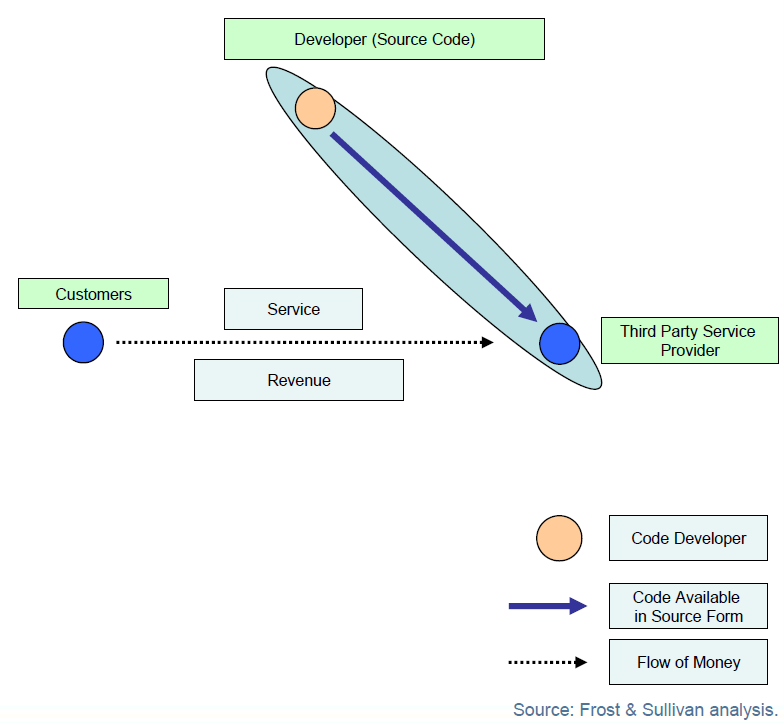
\includegraphics[width=.94\textwidth]{Impact-img2.png}}
 \caption{The Third-Party Services Model}\label{fig:tps-model}
\end{figure}

\begin{enumerate}
\item The \textbf{GPL model} (see Figure~\ref{fig:gpl-model}): With this model, the vendor
  is required to make the new code available in source form but it can choose to keep the
  new code as proprietary and charge for that proprietary software.  The vendor can
  provide the code commercially as part of a larger platform (hardware/software product)
  for which the companies receives revenue (license fee for the code + fees for technical
  support, updates and upgrades).
\item The \textbf{Third Party Service Model} (see Figure~\ref{fig:tps-model}) Many users
  may be willing to employ a third party service for distribution, modifications
  (debugging) and other support.
\end{enumerate}

\eucommentary{
Where relevant, include information on how the participants will manage
the research data generated and/or collected during the project, in
particular addressing the following issues: What types of data will the
project generate/-collect? What standards will be used? How will this
data be exploited and/or shared/made accessible for verification and
re-use (If data cannot be made available, explain why)? How will this
data be curated and preserved?}

\TODO{E.S. – Nicolas, ici je ne peux pas  écrire à ta place. Il faut juste que
tu répondes précisément aux questions posées ci-dessus.}

Open source software.


All software used and/or generated by the project will be Open Source.
This is a deliberate choice of the project consortium, as commercial
licenses (and patents) on this type of software only creates barriers
in our scientific domain.

Benefits of Open Source:

Acquisition and Costs: lower costs, easy access to the infrastructure,
lower risks of proprietary lock-in

Flexibility: picking up from Open Source projects, reduces dependence on
supplier, ability to view and modify the source code. Allows peer
reviewed modifications, community discussions. Open Source provides the
customer/end user the opportunity to innovate

Support: from developer community.

Besides being cost effective, Open Source software fosters
reuse, reliability, flexibility, and interoperability.

A consortium agreement will be established to manage ownership and
access to key knowledge, including software generated by the project.

Open access policy and data protection.

In line with the Horizon 2020 rules and current trends in IP
management and publication strategies, our consortium is committed to
open access publishing. This means that an article is immediately
provided in open access mode by the scientific publisher. As the
associated costs are usually shifted away from the readers, and
instead to the university or research institute to which the
researcher is affiliated, such costs have been accounted for by all
the research partner institutions. We have agreed to follow the
Guidelines on Open Access to Scientific Publications and Research Data
in Horizon 2020. In fact, following the now well established tradition
of the community, preprints for most publications will be posted on
\Arxiv.

Conforming to the call requirement, we will also participate in Open
research data pilot.  Following the Guidelines on Data Management in
Horizon 2020, we will establish a Data Management Plan, which first
version will be provided as an early deliverable in first six months of
the project. More developed versions of the plan will be provided as
additional deliverables at later stages.

Our strategy for knowledge management and protection includes measures
to provide open access (‘green' or ‘gold') to peer-reviewed scientific
publications and all data that may result from the project.

\subsubsection{Communication activities}
\label{subsubsect:communication}

\eucommentary{Describe the proposed communication measures for promoting the
project and its findings during the period of the grant. Where appropriate
these measures should include social media and public events with user
participation. Measures should be proportionate to the scale of the project,
with clear objectives. They should be tailored to the needs of various audiences,
including groups beyond the project's own community. Where relevant, include
measures for public/societal engagement on issues related to the project.}
%%% Local Variables:
%%% mode: latex
%%% TeX-master: "proposal"
%%% End:

%  LocalWords:  eucommentary programme subsubsection tablehead supertabular hline sur est
%  LocalWords:  e-infrastracture sémantique données amont j'ai mal si répond vraiment ce
%  LocalWords:  critère Systeme flushleft arraybslash Ergonomie il faut réflechir façon
%  LocalWords:  rendre l'outil attractif jeune génération génération des chercheurs va je
%  LocalWords:  définir donc terme Réfléchis possibilité tablettes mais aussi l'enseigner
%  LocalWords:  intéressante textgreater partie suivante demande elle ne serait mieux que
%  LocalWords:  unauthorised Maximise subsubsect organisational Pycon IPython Economie tu
%  LocalWords:  Standartisation Logiciel Libre includegraphics Impact-img1.png peux
%  LocalWords:  Impact-img2.png écrire répondes précisément posées ci-dessus


\clearpage

% ---------------------------------------------------------------------------
%  Section 3: Implementation
% ---------------------------------------------------------------------------

\section{Implementation}
\COMMENT{Typical granularity: 5-8 work packages with 3-5 tasks and one
  deliverable per task; 10 milestones}

\subsection{Work Plan --- Work packages, deliverables and milestones}
\label{sect:workplan}

\TOWRITE{ALL}{Proofread 3.1 work plan (except for the work packages themselves) pass 2}

\eucommentary{Please provide the following:\\
\begin{compactitem}
\item
brief presentation of the overall structure of the work plan;
\item
timing of the different work packages and their components (Gantt chart or similar);
\item
detailed work description, i.e.:
\begin{compactitem}
\item
a description of each work package (table 3.1a);
\item
a list of work packages (table 3.1b);
\item
a list of major deliverables (table 3.1c);
\end{compactitem}
\item
graphical presentation of the components showing how they inter-relate (Pert chart or similar).
\end{compactitem}
}

\subsubsection{Overall Structure of the Work Plan}\label{sec:workplan-structure}
\ifgrantagreement
The
\else
As shown in Figure~\ref{fig:wplist}, the
\fi
work plan is broken down into
seven work packages: \WPref{component-architecture} about components,
\WPref{UI} for user interfaces, \WPref{hpc} for parallelisation of the
components, \WPref{dksbases} for databases and finally
\WPref{social-aspects} for social aspects. This is complemented by the
the usual management and dissemination work packages
(\WPref{management}) and (\WPref{dissem}). The Gantt chart on
Page~\pageref{fig:gantt} illustrates the timeline for the various
tasks for these work packages%., including inter-task dependencies.

\ifgrantagreement\else
%\makeatletter\wp@total@RM{management}\makeatother
\wpfigstyle{\footnotesize\def\tabcolsep{3.5pt}}
%\wpfig[pages,type,start,end]
{\wpfig}
\fi
%\newpage
\subsubsection{How the Work Packages will Achieve the Project Objectives}
\label{sssec:how_the_work_packages_will_achieve}

% (Section~\ref{sect:objectives},page~\pageref{sect:objectives})

The following table recalls the objectives of \TheProject and lists
the work packages that contribute to achieving each of them.

\begin{center}
\begin{tabular}{|l|l|l|}\hline
\textbf{Objective} & \textbf{Purpose} & \textbf{WPs} \\\hline \hline
Objective 1
 & Develop and standardise math soft and data for VRE
 & \WPref{component-architecture},  \WPref{UI}, \WPref{hpc}, \WPref{dksbases} \\\hline
Objective 2
 & Develop core VRE components
 & \WPref{component-architecture}, \WPref{UI}, \WPref{hpc}, \WPref{dksbases} \\\hline
Objective 3
 & Bring together communities
 & \WPref{dissem}, \WPref{component-architecture} \\\hline
Objective 4
 & Update a range of softwares
 & \WPref{component-architecture}, \WPref{hpc} \\\hline
Objective 5
 & Foster a sustainable ecosystem
 & \WPref{component-architecture}, \WPref{UI}, \WPref{hpc}, \WPref{dksbases} \\\hline
Objective 6
 & Explore social aspects
 & \WPref{social-aspects} \\\hline
Objective 7
 & Identify and extend ontologies
 & \WPref{dksbases} \\\hline
Objective 8
 & Effectiveness of the VRE
 & \WPref{dissem}, \WPref{social-aspects} \\\hline
Objective 9
 & Effective dissemination
 & \WPref{dissem}, \WPref{social-aspects} \\\hline
\end{tabular}
\end{center}

\TOWRITE{ALL This next section is freshly rewritten to be more
  detailed. It doesn't show or explain dependencies between WPs or
  anything like that, which would be nice, but would take too
  long. Anyway please check}

\paragraph{Work Programme for Objective 1: }

\taskref{component-architecture}{interface-systems} (Interfaces
between Systems) directly addresses the core of objective 1, making
existing systems compatible with one another in mathematically sound
ways. Other tasks in \WPref{component-architecture} (component
architecture) support this, by making components more portable and
easier to deploy (\taskref{component-architecture}{mod-packaging}:
Modularisation and Packaging;
\taskref{component-architecture}{portability}). \taskref{component-architecture}{extract-smc}
will bring us the benefit of lessons learned and components built for
\SMC. \taskref{dksbases}{data-design} deals with the data-centric
aspects of the interfaces. Additionally elements of \WPref{UI} (user interface) and \WPref{hpc} (HPC)
will also contribute to the framework with user interface pluggability
and interfaces optimised for HPC.

\paragraph{Work Programme for Objective 2: }

We have identified a need for a number of new core components for
\TheProject and planned their construction at appropriate stages of
various workpackages. A new adapter infrastructure is part of
\taskref{component-architecture}{interface-systems}; new virtual
appliances will be built in
\taskref{component-architecture}{portability}; new components will be
extracted from \SMC in  \taskref{component-architecture}{extract-smc};
new documentation components will be developed in
\taskref{UI}{sage-sphinx} and \taskref{UI}{dynamic-inspect}; new
mathematical software will be developed in \taskref{hpc}{hpc-combi}
and new database tools in \taskref{dksbases}{data-memo} and \taskref{dksbases}{mws}.


\paragraph{Work Programme for Objective 3: }

Representatives of a number of communities have already come together
simply to prepare this proposal, and the whole project will work to
bring them together. Specifically developers of many systems  will be brought together to complete
work package~\WPref{component-architecture},
especially~\taskref{component-architecture}{interface-systems}.
Bringing broader communities together is the core purpose of
work package~\WPref{dissem}, which includes workshops, web sites,
demonstrator packages and outreach activities.

\paragraph{Work Programme for Objective 4: }

The concept of this project is centred on leveraging the communities
vast investment in existign open source software systems, and wherever
possible we will proceed by extending and updating existing software components.
In work package \WPref{component-architecture} we will address
portability (\taskref{component-architecture}{portability} and
modularity (\taskref{component-architecture}{extract-smc}) and also
adapt the components to use the new interfaces being designed in
\taskref{component-architecture}{interface-systems}. Work package
\WPref{hpc} is largely about updating software for performance, while
workpackage \WPref{UI} deals with adaptation of UI components and of
other systems to work with them.

\paragraph{Work Programme for Objective 5: }

A number of tasks relate to developing promoting and supporting
sustainable models for collaborative software development. On a
practical level \taskref{component-architecture}{workflow} will adress
processes and technologies, \taskref{dksbases}{data-memo} concerns
collaborative accumulation of data. On a personal level, much of
\WPref{dissem} deals with ensuring a wide and committed user/developer
community. Finally in~\taskref{social-aspects}{isocial-decisionmaking}
we will actually conduct research into the social mechanisms of
collaborative software development, and lessons from this research
will be embedded into the structures we leave behind.

\paragraph{Work Programme for Objective 6: }

Objective 6 is covered by a dedicated work package \WPref{social-aspects} on social aspects.
It ranges from analysis of the needs with~\taskref{social-aspects}{social-input} to
evaluation with~\taskref{social-aspects}{oommf-nb-evaluation}.

\paragraph{Work Programme for Objective 7: }

Objective 7 is addressed directly by \WPref{dksbases}, which deals with data
and its meaning.

\paragraph{Work Programme for Objective 8: }

Producing and evaluating systems that demonstrate our achievements is
a key feature of this project, and this work in embedded throughout
the project. The integration and publicisation of these demonstrators
is key to \WPref{dissem} (dissemination) especially later in the
project, while their formal evaluation is found in \WPref{social-aspects}.

\paragraph{Work Programme for Objective 9: }

Dissemination is the heart of~\WPref{dissem}.
Members of \TheProject will organise workshops within \taskref{dissem}{dissemination}
or \taskref{dissem}{project-intro} as well as less formal meetings
with interested groups. In addition, we will follow open software development
processes throughout the project, so that our work is immediately
available to any interested party. We will announce important
developments or releases through our own web pages and the
established channels of the component systems. Our scientific findings
will be published in the open scientific literature and announced at
scientific meetings and conferences in the usual way and reported in
annual project reports.


\subsubsection{Work Plan Timing: GANTT Chart showing Task Dependencies and Information
  Flows}

Since \TheProject consists mainly in improving independent tools and
integrating them into a VRE, its tasks are fairly independent from each
other, which is reflected by the GANTT chart in Figure~\ref{fig:gantt}

\gantttaskchart[draft,xscale=.33,yscale=.33,milestones]

\ifgrantagreement\else
\newpage
\subsubsection{Deliverables}\label{sec:deliverables}
\inputdelivs{9.3cm}
\fi

\newpage
\subsubsection{Milestones}\label{sec:milestones}
\eucommentary{Milestones means control points in the project that help to chart progress. Milestones may
correspond to the completion of a key deliverable, allowing the next phase of the work to begin.
They may also be needed at intermediary points so that, if problems have arisen, corrective
measures can be taken. A milestone may be a critical decision point in the project where, for
example, the consortium must decide which of several technologies to adopt for further
development.}

The work in the \TheProject project is structured by four milestones,
which coincide with the four project meetings held at the end of each
year of the project (the other four meetings will be held in the middle
of each year). Given the nature of the project, with a
large number of essentially independent tasks, there is no need for
milestones attached to specific collections of tasks or
deliverables. Instead, given that the meetings are the main
face-to-face interaction points in the project, it's suitable to
schedule the milestones for these events, where they can be discussed
in detail, tracking the progress in each work package through status
reports on the tasks and deliverables.

We envisage that this setup will give the project the vital coherence
in spite of the broad interdisciplinary mix of various backgrounds of the
participants.

% \newcommand{\WPall}{\WPref{management}, \WPref{dissem}, \WPref{component-architecture}, \WPref{UI}, \WPref{hpc}, \WPref{dksbases}, \WPref{social-aspects}}

% \newcommand{\WPnoUI}{\WPref{management}, \WPref{dissem}, \WPref{component-architecture}, \WPref{hpc}, \WPref{dksbases}, \WPref{social-aspects}}

% \begin{center}
%   \begin{tabular}{|m{.05\textwidth}|m{.30\textwidth}|m{.15\textwidth}|m{.05\textwidth}|m{.22\textwidth}|}
%     \hline
%     Mile-stone nr. & Milestone name & Related work packages & Est. date & Means of verification \\\hline
%     M1 & Requirements study, design and prototype implementations. Start of
%          community building.
%        & \WPall 
%        & 12 
%        & 2nd Project meeting report. Completion of corresponding deliverables. \\\hline
%     M2 & First fully functional interface implementations.
%          Enhanced versions of \TheProject components.
%          Training early adopters.
%        & \WPall 
%        & 24 
%        & 4th Project meeting report. Completion of corresponding deliverables. \\\hline
%     M3 & Evaluating \TheProject software. Working with the community 
%          and building portfolio of experiments produced with \TheProject.
%        & \WPall 
%        & 36 
%        & 6th Project meeting report. Completion of corresponding deliverables. \\\hline
%     M4 & Project evaluation and final versions of all \TheProject components.
%        & \WPnoUI 
%        & 48 
%        & 8th Project meeting report. Completion of corresponding deliverables. \\\hline
%   \end{tabular}
% \end{center}

\begin{milestones}
  \milestone[id=startup,month=12,
  verif={Completed all corresponding deliverables and reported the progress in the 2nd Project meeting report.}]
  {Startup}
  {By Milestone 1 we will have carried out the requirements study, design and prototype implementations and started community building activities.}

  \milestone[id=proto1,month=24,
  verif={Completed all corresponding deliverables and reported the progress in the 4th Project meeting report.}]
  {Prototypes}
  {By Milestone 2 we will have constructed first fully functional interface implementations and released enhanced versions of \TheProject components, and train early adopters of \TheProject.}

  \milestone[id=community,month=36,
  verif={Completed all corresponding deliverables and reported the progress in the 6th Project meeting report.}]
  {Community/ Experiments}
  {By Milestone 3 we will have gathered and evaluated feedback on \TheProject software and established the portfolio of experiments produced with \TheProject through further engaging with the community.}

  \milestone[id=eval,month=48,
  verif={Completed all corresponding deliverables and reported the progress in the 8th Project meeting report.}]
  {Evaluation}
  {By Milestone 4 we will have released final versions of all \TheProject components and completed the project evaluation.}
\end{milestones}

%%% Local Variables:
%%% mode: latex
%%% TeX-master: "proposal"
%%% End:

%  LocalWords:  verif ldots


% ---------------------------------------------------------------------------
% Include Work package descriptions
% ---------------------------------------------------------------------------

%% WP titles and order are defined in deliverables.tex
%%% Workpackage style may be broken -- fix this!!

%% Local WP number counter - should possibly be global and hidden?

\newcounter{wpno}

\begin{workpackage}[id=management,type=MGT,wphases=0-48!.2,
  title=Project Management,short=Management,
  lead=PS,
  PSRM=48,SARM=48,USORM=2]

\begin{wpobjectives}
  The objectives of this work package are to undertake all project management activities,
  including:
  \begin{compactitem}
  \item monitoring the overall progress of the project and the use of
    resources;
  \item ensuring the timely production of deliverables and other
    project outputs;
  \item reporting to the European Commission on financial matters;
  \item preparing for and attending the annual project review
    meetings; and
  \item managing the project Advisory Board.
  \end{compactitem}

  % The objective of  is to undertake all project management
  % activities, including setting up joint infrastructure, organizing
  % meetings, and producing overview reports.
\end{wpobjectives}

\begin{wpdescription}
  This workpackage will perform all the activities related to monitoring of progress
  towards the project milestones shown on Page~\pageref{sec:milestones} and the
  deliverables listed on Page~\pageref{sec:deliverables}, assuring the quality of the
  deliverables, ensuring the collation and distribution of the required reports,
  questionnaires and deliverables including the annual reports to the European Commission,
  arranging project management meetings, tracking the project budget in terms of
  expenditure and person-months, obtaining financial certificates as required, convening
  project management meetings, ensuring that important project documents such as the
  project contract and the consortium agreement are properly maintained and amended as
  necessary, ensuring that contractual details are complied with, monitoring compliance
  with the grant agreement, preparing for the annual review meetings, and reviewing
  research results against the aims and objectives of the project. It also involves
  managing and supporting the project Advisory Board, including supporting attendance at
  project meetings, convening Advisory Board meetings, and obtaining feedback on the
  project direction and results.
\end{wpdescription}

\TODO{MK: I would combine the first three into one ``basic project infrastructure''}
\begin{wpdelivs}
\begin{wpdeliv}[due=1,id=tickets,dissem=PU,nature=DEC]{Create tickets for all relevant tasks / deliverables}
\end{wpdeliv}
\begin{wpdeliv}[due=1,id=mailinglists,dissem=PU,nature=DEC]{Internal and external mailing lists}
\end{wpdeliv}
\begin{wpdeliv}[due=1,id=swrepository,dissem=PU,nature=DEC]{Internal software repository}
\end{wpdeliv}
\begin{wpdeliv}[due=12,id=periodic-rep-1,dissem=PU,nature=R]{Project Periodic Report (first year)}
 \end{wpdeliv}
\begin{wpdeliv}[due=24,id=periodic-rep-2,dissem=PU,nature=R]{Project Periodic Report (second year)}
 \end{wpdeliv}
\begin{wpdeliv}[due=36,id=periodic-rep-3,dissem=PU,nature=R]{Project Periodic Report (third year)}
 \end{wpdeliv}
\begin{wpdeliv}[due=48,id=periodic-rep-4,dissem=PU,nature=R]{Project Periodic Report (fourth year)}
 \end{wpdeliv}
\begin{wpdeliv}[due=48,id=final-mgt-rep,dissem=PU,nature=R]{Project Final Report}
 \end{wpdeliv}
\end{wpdelivs}
\end{workpackage}
%%% Local Variables: 
%%% mode: latex
%%% TeX-master: "../proposal"
%%% End: 

%  LocalWords:  workpackage wphases wpobjectives wpdescription pageref wpdelivs wpdeliv
%  LocalWords:  dissem mailinglists swrepository final-mgt-rep compactitem

\begin{workpackage}[id=community,wphases=5-36!.7,
%<<<<<<< HEAD
title=Community Building and Engagement,
SARM=1,USHRM=8]
%=======
%  title=Community Building and Engagement,
%  lead=PS,
%  PSRM=12,SARM=1,USHRM=8]
%>>>>>>> e490abbfa8a91427570f1a7695a6a95cd4610713

\begin{wpobjectives}
  The objective of this work package is to further develop the community at the
  European scale, foster cross teams collaborations, spread the
  expertise, and engage the greater community to participate to the
  definition of the needs, and the implementation and use of the
  produced solutions.
% \begin{itemize}
% \item
% \item
% \item
% \item
% \item
% \end{itemize}
\end{wpobjectives}

\begin{wpdescription}
  We will organize regular open workshops (e.g. Sage Days, Pari Days,
  summer schools, etc.); some of them will be focused on development
  and coding sprints, and others on training.

\TODO{Neil: I have a series of Gaussian process summer schools and road shows that I'rm organizing. These will also shift to more of a focus on data science across this year, I'd be happy to include these here if that's appropriate.}

  This work package will also provide general travel budget to fund
  short to long term visits between the participants, to collaborate
  on specific features. A typical such visit would bring together an
  IPython developer with a GAP developer for a couple of days to
  implement a first prototype of notebook interface to GAP.

  This work package will complement and lean on a parallel COST
  network whose role is to build and animate the greater community.


\end{wpdescription}

\begin{wpdelivs}
  \begin{wpdeliv}[due=6,id=ws1,dissem=PU,nature=O]{Workshop 1}
  \end{wpdeliv}
  \begin{wpdeliv}[due=12,id=needs,dissem=PU,nature=R]{Report on community needs}
  \end{wpdeliv}
  \begin{wpdeliv}[due=18,id=ws2,dissem=PU,nature=O]{Workshop 2}
  \end{wpdeliv}
  \begin{wpdeliv}[due=30,id=ws3,dissem=PU,nature=O]{Workshop 3}
  \end{wpdeliv}
  \begin{wpdeliv}[due=42,id=ws4,dissem=PU,nature=O]{Workshop 4}
  \end{wpdeliv}
\end{wpdelivs}
\end{workpackage}
%%% Local Variables:
%%% mode: latex
%%% TeX-master: "../proposal"
%%% End:

\addtocounter{wpno}{1}
\begin{Workpackage}{\thewpno}
\wplabel{wp:x}
\WPTitle{\wpname{\thewpno}}
\WPStart{Month 1}
\WPParticipant{SA}{1}

\begin{WPObjectives}
  The objective of \theWP{} is to produce periodic reviews of relevant
  developments elsewhere and implications for our plans, including
  negotiating access or shared development when appropriate.

  It will feed this information to the other work packages, in
  particular\TODO{ref: Component Architecture}.
\end{WPObjectives}

\begin{WPDescription}
  This workpackage  ...

  \begin{itemize}
  \item Review standard components/service for storage and sharing,
    computational resources, authentication, package management, etc.
  \end{itemize}
\end{WPDescription}

\begin{WPDeliverables}
\begin{itemize}
\item
\ref{del:periodic-rep-1}
(Month 12): Year 1 report.
\item
\ref{del:periodic-rep-2}
(Month 12): Year 2 report.
\item
\ref{del:periodic-rep-3}
(Month 12): Year 3 report.
\item
\ref{del:periodic-rep-4}
(Month 12): Year 4 report.
\end{itemize}
\end{WPDeliverables}
\end{Workpackage}

\TOWRITE{ALL}{Proofread WP 3 Component Architecture pass 2}
\begin{draft}
\TOWRITE{UV (Work Package Lead)}{For WP leaders, please check the following (remove items
once completed)}
\begin{verbatim}
- [X] have all the tasks in this Work Package a lead institution?
- [X] have all deliverables in the WP a lead institution?
- [X] do all tasks list all sites involved in them?
- [X] does the table of sites and their PM efforts match lists of sites for each task?
      (each site from the table is listed in all relevant tasks, and no site is listed
      only in the table or only at some task)
\end{verbatim}
\end{draft}

\begin{workpackage}[id=component-architecture,wphases=0-48!.5,
  title=Component Architecture,lead=UV,
  PSRM=64,UVRM=8,SARM=16, USORM=6, UORM=4, LLRM=14, UJFRM=6]
  % PS: Full time dev: 48 PM, NT: 4 PM

  \begin{wpobjectives}
    The objective of this work package is to develop and demonstrate a
    set of APIs that enable components, such as database interfaces,
    computational modules, separate systems such as \GAP or \Sage, to
    be flexibly combined and run smoothly across a wide range of
    environments (such as Cloud-based, local, and server environments).
  \end{wpobjectives}

  \begin{wpdescription}
    This Work Package focuses on the structure of the components that make
    up a mathematical software and their interactions. Such components
    can be separate modules inside a unique software, or separate
    softwares interacting through library calls and/or through APIs
    (e.g.: web APIs). When combined together, they make up a full VRE.

    The architecture of these software components must be:
    \begin{compactitem}
    \item \textbf{Portable}, to support a wide range of platforms
      (mobile, desktops, cloud, \dots).
    \item \textbf{Modular}, so to ease installing, building, testing,
      and remixing.
    \item \textbf{Flexible}, so to adapt to different use cases:
      personal computation, HPC, parallel platforms, \dots
    \item \textbf{Open}, in the sense of \emph{open source}, but also
      in the sense of clearly documented and open to
      the user who wants to understand its underpinnings and/or
      contribute to it. Indeed we must not forget that the working
      mathematicians and other users need to know what algorithms the software is
      going to run to solve a given problem.
    \end{compactitem}
  \end{wpdescription}

  \begin{tasklist}
  \begin{task}[id=portability,title=Portability,lead=UV,PM=28,partners={PS},wphases=0-36]
    In order to achieve maximum availability and accessibility,
    mathematical software must be developed and tested for a wide range
    of computer architectures and operating systems.  However most of
    open source development happens in POSIX environments (usually
    Linux or OS X), and almost exclusively on x86 platforms.  The vast
    majority of the developers of mathematical software does not have
    the expertise, nor the access to appropriate hardware and software, to insure
    appropriate testing and porting of components.  The best
    incarnation of this issue is the involved installation procedure
    for \Sage on Windows, a major adoption barrier and common source of
    complaints by end-users.

    In this task we will address the common needs of the community in
    terms of portability layers, building and testing infrastructure.

    \begin{compactitem}
    \item Best practices adopted by the larger open source community
      will be investigated and leveraged, and existing expertise will
      be shared between the component developers.
    \item Windows being largely dominant in the desktop/laptop market,
      a specific focus will be placed on the port of \Sage, and
      therefore all the components included in its distribution (in
      particular \PariGP, \GAP, \Singular, \Linbox) to this platform
      (\delivref{component-architecture}{portability-cygwin32},
      \delivref{component-architecture}{portability-cygwin64}).
    \item The deployment of a common infrastructure for multi-platform
      continuous integration (testing, building and distribution) will
      be addressed
      (\delivref{component-architecture}{multiplatform-buildbot}).
    \end{compactitem}

      % Jean-Pierre:
      % Should we mention port to non-x86-64 archs and non-Linuces?
      % 
      % For CPUs:
      % - I guess at least ARM and ppc64 (IBM POWER*) really make sense.
      % - Sparc is less convincing though the latest sparc CPUs
      % are muche more interesting for math computation as the
      % previous ones, e.g. the GMP folk specifically added assembly
      % for them in their latest release.
      % - Itanium is dead, but it can help discovering bugs as any non
      % standard archs.
      % - Supporting any of these would mean buying (potentially very
      % expensive) hardware.
      % 
      % For OSes?
      % - Should we mention OS X which is a pain at each new release?
      % - A BSD variant would be interesting, let's say FreeBSD which
      % is basically (almost) already supported
      % - Solaris? and/or OpenIndiana? Interesting if we mention sparc...
      % - Windows is already included below, my opinion is:
      % * provide live USB, VMs and Cygwin32 first as these three are
      % basically already working solutions
      % * go Cygwin64 as it is still POSIX
      % * explorate a MinGW solution, at least GAP and PARI should be
      % problematic
      % * try to use MSVC
  \end{task}

  \begin{task}[title=Interfaces between systems,id=interface-systems,lead=PS,PM=22,partners={UV,UO,SA},wphases=0-36]
    In this task we will investigate patterns to share data,
    ontologies, and semantics across computational systems, possibly
    connected remotely.  We will leverage the well established
    semantics used in mathematics (categories, type systems, \dots) to
    give powerful abstractions on computational objects.
    
    We will build upon the work already done in the EU FP6 project
    26133 ``SCIEnce -- Symbolic Computation Infrastructure for
    Europe'' (\url{http://www.symbolic-computing.org/}) on the Symbolic Computation
    Software Composability Protocol (SCSCP). SCSCP is a remote
    procedure call protocol by which a computer algebra system (CAS)
    may offer services to a variety of possible clients, including
    e.g.  another CAS running on the same computer system or remotely;
    another instance of the same CAS (in a parallel computing
    context); a simplistic SCSCP client
    (e.g. C/C++/Python/etc. program) with a minimal SCSCP support
    needed for a particular application; a Web server which passes on
    the same services as Web services, etc.  A distinctive feature of
    the protocol is that both instructions and data are represented in
    the OpenMath format (\url{http://www.openmath.org/}; previously
    supported by the EU JEM Thematic Network; EU project 24969
    ``ESPRIT'' and other projects); moreover, OpenMath support is not
    limited by existing official OpenMath content dictionaries --
    private encodings may be easily embedded into SCSCP messages.
    
    SCSCP is already supported by a number of computer algebra
    systems, including \GAP, Macaulay2, Maple, TRIP and others. We
    will extend support for SCSCP to other relevant systems involved
    in \TheProject (\delivref{component-architecture}{scscp-sage}).
    Through its API, we will enable discovery of subsystems,
    functionality, documentation and computational resources. The user
    interfaces shall be enabled to automatically choose the best
    available algorithms and resources to perform a required
    computation, as well as clearly and intuitively present the
    available choices to the expert user.

    As a first concrete test bed, we will consider the \Sage interface
    to \GAP, or more precisely \libGAP.  Like most \Sage interfaces,
    this uses the now classical \emph{handle} design pattern, whereby
    one can manipulate from \Sage an object created and stored in
    \GAP, through a \emph{handle} (a.k.a. \emph{remote objects}).  By
    mapping \GAP's categories to \Sage's categories, in
    \delivref{component-architecture}{semantic-interface-sage-gap} we
    will:
    \begin{compactitem}
    \item Implement a modular infrastructure for adapters, based on
      SCSCP, in order to let the implementation of adapters scale to a
      large variety of objects.
    \item Refactor the existing adapters, using this infrastructure to
      generalise their features. This step by itself will provide
      adapters for larger categories like semigroups or monoids.
    \item Merge the adapters into the handles, so that a handle to a
      \GAP group will \emph{automatically} behave like a native \Sage
      group.
      % This will remove much back-conversion burden from the
      % delegating methods
    \end{compactitem}
    A specific challenge will be performance; indeed low level method
    adapters, e.g. for arithmetic, need to be compiled when most of
    the interface infrastructure is dynamic by nature.

    % When different algorithms are available, some of them coded in
    % \Sage, some of them in \GAP, the interface shall offer an easily
    % navigable interface for the expert user to choose among them.
  \end{task}

  \begin{task}[title=Modularisation and packaging,id=mod-packaging,lead=UV,PM=20,partners={PS,LL},wphases=0-48]
    % TODO: logilab can contribute to producing VM images
    % using its proven worflow based on saltstack and packer.io PM=2
    % TODO: logilab can help to define the metadata to be provided
    % by software authors to facilitate the packaging of their
    % components. Beware not the reinvent the wheel^H packaging system.
    % PM=2
    % TODO: if needed, logilab can develop a package index similar
    % to PyPI using CubicWeb: html UI for browsing and web service
    % for registration. Maybe an instance of PyPI is enough? PM=6
    % TODO: logilab can help with debian packages PM=6
    In this task we will investigate best practices for composing,
    sharing and interfacing computational components and data for
    connected mathematical systems.

    We will start with a comparative study of the practices adopted in
    various open source projects, both inside and outside of
    \TheProject. This will include reviewing non-mathematical systems,
    e.g.: operating systems, platforms, web frameworks, cloud and HPC
    infrastructures.  In particular, pushed by cloud computing,
    containerisation \cite{Docker} and virtualisation
    \cite{Virtualbox} have become a major trend for distributing
    complex software, thanks to their ease of installation and
    configuration. We shall experiment with these technologies by
    building and distributing virtual appliances for the major
    components of \TheProject
    (\delivref{component-architecture}{virtual-machines}).

    Once the initial study will have identified the present
    shortcomings, we will promote a new generation of mathematical
    software that is capable of scaling to large code bases, large
    datasets, and massively distributed infrastructures. This task
    also needs to consider the results of work
    package~\WPref{social-aspects} on social issues regarding
    distributed development, community management, acknowledging
    contributions, etc.

    As an example, \Sage has a long history of integrating and
    distributing large mathematical libraries/software as a whole,
    with relatively few attention given to defining and exposing
    interfaces. Component re-usability is not a main focus for the
    \Sage community, at the same time the non-standard and relatively
    underused package system discourages writing and maintaining
    autonomous libraries. These factors have contributed to make the
    \Sage distribution what is usually described as a ``monolith''
    (\Sage library code alone, not counting included libraries, makes
    up for 1.5M lines of code and documentation), hard to distribute,
    to maintain, to port, and to develop with.

    On the other hand, \GAP has been distributing
    community-developed ``\GAP packages'' for a long time, but faces
    now fragmentation issues, at the code and at the community
    level. The rudimentary package system adds more technical
    difficulties to \GAP's development model.

    Both models reach the limits of their scalability, and a synthesis
    is very much needed.  Our first experiment will be to enhance
    \Sage's package system
    (\delivref{component-architecture}{sage-repository}), enough to
    support an open repository of user-contributed code, in the same
    spirit of modern systems such as Julia
    (\url{http://pkg.julialang.org/}) or PyPI
    (\url{https://pypi.python.org/}).  Once \emph{internal} packaging
    has been dealt with, the route will be paved to further modularise
    the \Sage distribution, and make sure that the major Linux
    distributions have standard packages for it
    (\delivref{component-architecture}{sage-distribution}).

  \end{task}

\begin{task}[id=simulagora-dev,title=Simulagora integration,PM=4,lead=LL,wphases=0-48]
  To deliver every six month a new Simulagora VM image containing all the software
  components released over the period. The goal is to prove that the project is
  improving the component architecture by measuring the time it takes to
  integrate them.
\end{task}


  \begin{task}[title=Component architecture for High Performance Computing and Parallelism,id=component-for-HPC,PM=12,wphases=36-48,lead=UJF,partners=SA]
    As in all other areas of science, properly supporting massively
    parallel architecture is a major challenge. Many of the
    computational components have already gone a long way in this
    direction, and further work will be carried out in
    WorkPackage~\WPref{hpc}.

    In this task we will investigate and implement
    parallelism-friendly ways of combining components together, so
    that calling components can benefit from the parallelism features
    of called components, with self-adaptation to the environment and
    cooperative sharing of resources. We will use \Sage and its
    components as a test-bed, by producing an HPC-enabled distribution
    (\delivref{component-architecture}{hpc-configure}).
  \end{task}

  \begin{task}[title=Document and modularise \SMC's codebase,id=extract-smc,lead=PS,PM=10,partners={UV},wphases=0-24]
    From its inception in 2013, \SMC\ (see Section~\ref{linked-projects}, page~\pageref{sec:SMC-page}) 
    has quickly developed into a full
    featured VRE.  Because of the tight, partly closed source
    development cycles, \SMC's codebase has quickly grown in size,
    with its documentation not always keeping the pace. As a result,
    it is at the moment very hard for a newcomer to set up a clone
    service of \SMC just from its sources.

    Now that \SMC is
    \href{https://twitter.com/sagemath/status/544939872294014977}{fully
      open source}, we need to go through its codebase, understand and
    document it
    (\delivref{component-architecture}{smc-documentation}), isolate
    components that might be reused by other software (e.g.:
    \Jupyter), and make it as portable as possible.

    The ultimate goal of this task is to produce a \emph{personal}
    version of \SMC, to be shipped along with \Sage, that a user can
    run on his own personal computer
    (\delivref{component-architecture}{personal-smc}).
  \end{task}

  \begin{task}[title=Improving the development workflow in mathematical software,id=workflow,lead=UV,PM=10,partners={PS,LL},wphases=6-24]
    Truly open software must enable any actor to easily contribute his
    work to the community. Be it an experienced developer, or a
    student. Be it for a major software component or for a piece of
    translation. All the systems involved in \TheProject have
    developed their own workflows for contributing back, but those are
    almost exclusively geared toward experienced developers working on
    large components. When these workflows eventually reach their
    scalability limits, software development stagnates and major
    features are delayed. A well known example is given by \Sage's TRAC
    server, where tickets can stay in ``needs review'' state for a
    long time before entering the code base.  \emph{Upstream} bug
    reporting and fixing is another major factor of slow development.

    This task will seek new ways of accepting contributions to
    mathematical software in a scalable way. For example we will
    experiment with integrating bug reporting and contributing
    features right in the VRE (e.g., in \SMC:
    \delivref{component-architecture}{smc-trac}).).

    % TODO: logilab would like to enhance the existing forges to publish
    % linked open data and ease the sharing of information about
    % package/version/issues across systems. See for example
    % https://packages.qa.debian.org/p/python-defaults.html and the link to RDF
    % meta-data on the right
    % https://packages.qa.debian.org/p/python-defaults.ttl
    % see also https://wiki.debian.org/RDF
    % PM=6 up to 12
  \end{task}


\begin{task}[lead=USO,id=oommf-python-interface,title=Python interface for OOMMF micromagnetic simulation library,PM=6,wphases=3-9,partners={SA}]
  % 6 person months
  In this task, we create a Python interface
  (\delivref{component-architecture}{oommf-py}) for the open source Object
  Oriented MicroMagnetic Framework (OOMMF \cite{OOMMF-url}).
  %which is the most widely used micromagnetic simulation package
  %\cite{OOMMF-citations-url}. 
  As a result, the OOMMF library will be fully accessible and usable
  from a Python interface and become a component in the
  Python/\Jupyter eco system of computational tools and in
  \TheProject. We make use of this component architecture in
  \taskref{UI}{oommf-py-ipython-attributes} to build the micromagnetic
  VRE demonstrator
  (Sect.~\ref{sec:introduction-micromagnetic-vre-demonstrator}).

  In more detail, we will first identify the best option for interfacing
  from Python to OOMMF core (C++) routines. The technical options
  include CTypes, Cython, Swig, and Boost-Python, all with particular
  advantages/disadvantages. Following analysis of the current OOMMF
  code layout and compilation model, we will use the most suitable
  tool, bearing in mind our ambition not to modify the OOMMF code so
  that the python interface we create remains functional and
  maintainable with minimal effort while the OOMMF core code is
  developed further by the OOMMF authors. 
  The interface will expose the C++ objects in Python, providing
  an architecture component that provides full access to OOMMF's
  raw capabilities. For clarity, we will refer to this interface as
  \texttt{OOMMF-py-raw}. %Creation of this \texttt{OOMMF-py-raw} is
  %technically doable as OOMMF had been written allowing to do this
  %from Tcl. The \texttt{OOMMF-py-raw} library for Python provides
  %access to the OOMMF functionality but requires some care when being
  %used.

  Secondly, we will create a user friendly Python library
  \texttt{OOMMF-py} that combines the \texttt{OOMMF-py-raw}
  capabilities in an object orientated and safe-to-use Python library
  targeting researchers in the magnetic materials community. We will
  follow the design of the well-received high level Python interface
  in the Nmag micromagnetic simulation package \cite{Fischbacher2007a}
  interface \cite{Nmag-url}. Unit and regression tests for both
  component interfaces \texttt{OOMMF-py-raw} and \texttt{OOMMF-py} are
  simultanously developed.

  %Once this is completed, several new features will be available to
  %OOMMF users: (i) ability to drive OOMMF from Python, (ii)
  %computational steering, and (iii) combination of OOMMF simulation
  %with the existing Python eco-system of computational tools.

  %Can remove the next paragraph if we are pushed for space.

  %We illustrate the advantage of (iii) through an example: to solve
  %the micromagnetic standard problem 3
  %\cite{Micromagnetic-Standardproblem-3}, traditionally multiple OOMMF
  %simulation runs would have to be conducted, and for each of those a
  %new configuration file as to be written. Between these the size of
  %the simulated geometry needs to be modified until two particular
  %values of energy are the same. Given the new interface developed in
  %this work package, this whole process can be replaced by one Python
  %script that creates multiple OOMMF simulations, combined with a root
  %finding method for the automatic iterative determination of the
  %required simulation geometry.

  %For all tasks relating to
  %\OOMMFNB, documentation and tests are created simultaneously with
  %the code. All codes, tests and documentation will be made available as open source.

  %We anticipate to start this task \localtaskref{oommf-python-interface}
  %in month 4, leading to deliverable \delivref{UI}{oommf-py}.
\end{task}





\end{tasklist}

  \begin{wpdelivs}
    \begin{wpdeliv}[due=6,miles=startup,id=portability-cygwin32,dissem=PU,nature=OTHER,lead=UV]
      {One-click install \Sage distribution for Windows with Cygwin 32bits}
      % JPF: this should take a few months of work
      % This 32bits version would work right away on Windows 64 bits with
      % Cygwin 32 bits; more work would be required for a version working on
      % a 64 bits of Cygwin.
      % JPF: I agree.
    \end{wpdeliv}%


    \begin{wpdeliv}[due=6,miles=startup,id=virtual-machines,dissem=PU,nature=OTHER,lead=UV]
      {Virtual images and containers} Creation and distribution of
      preconfigured cloud oriented virtual machines/containers
      (e.g. Docker images) for \PariGP, \Sage, \SMC, \dots
      % Requires: licenses
      \TOWRITE{??}{Make this deliverable shorter.}
    \end{wpdeliv}
    \begin{wpdeliv}[due=6,miles=startup,id=smc-documentation,dissem=PU,nature=R,lead=PS]
      {Understand and document \SMC backend code.}
    \end{wpdeliv}%

    \begin{wpdeliv}[due=9,miles=startup,id=oommf-py,dissem=PU,nature=OTHER,lead=USO]
      {Python Interface to micromagnetic OOMMF package completed}
    \end{wpdeliv}


    \begin{wpdeliv}[due=12,miles=startup,id=scscp-sage,dissem=PU,nature=OTHER,lead=SA]
      {Support for the \href{http://www.symbolic-computing.org/}{SCSCP} interface protocol
        in all relevant components (\Sage, \GAP, etc.) distribution}
    \end{wpdeliv}

    \begin{wpdeliv}[due=24,miles=proto1,id=personal-smc,dissem=PU,nature=OTHER,lead=PS]
      {\emph{Personal} \SMC: single user version of \SMC distributed
        with \Sage.}
    \end{wpdeliv}%

    \begin{wpdeliv}[due=24,miles=proto1,id=smc-trac,dissem=PU,nature=OTHER,lead=UV]
      {Integration between \SMC and \Sage's TRAC server}
    \end{wpdeliv}
    \begin{wpdeliv}[due=24,miles=proto1,id=sage-repository,dissem=PU,nature=OTHER,lead=UV]
      {Open package repository for \Sage} Refactor \Sage package and
      build system to support community-contributed packages
      installable via the web.
    \end{wpdeliv}

    \begin{wpdeliv}[due=24,miles=proto1,id=portability-cygwin64,dissem=PU,nature=OTHER,lead=PS]
      {One-click install \Sage distribution for Windows with Cygwin 64bits}

      % Participants involved: Paris Sud, Kaiserslautern, Saint Andrews, Bordeaux
      % Comments on this by Bill Hart
      % The big problems you will have on Windows 64 on Cygwin include:
      % 
      % * anything with assembly language -- the ABI is different on Windows, so
      % it'll need rewriting, or you can incur a performance penalty by using
      % generic C fallback code
      % * the memory allocator on Windows is not so great
      % * bugs exposed due to being on a different platform, e.g. segfaults due to
      % off-by-one errors that were masked by the granularity of malloc on Linux
      % * build issues, due to identifying Cygwin and using the correct header
      % files, which are often different on Cygwin than linux
      % * issues with PATH vs LD_LIBRARY_PATH
      % * Windows has a case insensitive file system
      % * EOL issues
      % * Windows is not able to rapidly create and delete files, which some
      % libraries (esp. test code) calls for
      % * memory limitations (many people using Windows are using laptops with
      % limited memory, only a portion of which is realistically available to
      % Cygwin)
      % * autotools versions that don't support Windows (usually autotools has a
      % release that is used in all the distributions, which doesn't work correctly
      % on Windows, and this is followed up by a version which has all the Windows
      % patches)
      % * building takes forever on Windows. Mingw2 has now gotten parallel build
      % working on Windows and the speed is within a factor of 5 of Linux. But I'm
      % not sure the improvements have propagated to Cygwin yet.
      % * Cygwin 64 is new, contains quite a few bugs still, and things keep
      % changing with every version as they try to get things right.
      % * Although projects will likely accept patches for Windows, they are less
      % likely to maintain support themselves. I would like to think Singular would
      % be an exception to this. And obviously flint and MPIR work on Windows (even
      % with MSVC as of the next version of flint -- or now if you use our bleeding
      % edge repo version).
      % 
      % Comments by Jean-Pierre on some of the above and mor:
      % * first things first: I already completely built Sage on Cygwin64, though it
      % was surely not completely functional.
      % * assembly: that's right, note that as far as Sage and it's dependencies are
      % concerned, only a few of them actually use assembler, and yes all of them
      % provide fallback generic C code IIRC
      % * PATH vs LD_...: basically the same problem as for Cygwin32, so it's already
      % been taken care of for the Cygwin32 port
      % case issue: not a problem IIRC
      % * EOL issues: I don't thing so, Cygwin is POSIX like
      % * autotools issues: most of Sage dependencies are now updated, I used to track
      % the few problematic ones in 2013
      % * time to build: not so long, sure longer than on a POWER7 machine, but I do
      % it on a usual x86_64 laptop running Debian within a Windows VM in a few hours!
      % what we actually really need is patch/build bots to test on Cygwin 32/64!
      % * upstream cooperation: I agree Windows is often a low priority issue, but
      % most teams have welcomed my Cygwin patches
    \end{wpdeliv}

    \begin{wpdeliv}[due=36,miles=community,id=multiplatform-buildbot,dissem=PP,nature=DEM,lead=UV]
      {Continuous integration platform for multi-platform build/test.}

      \Sage's \emph{buildbot} is a x86\_64/Linux specific platform for
      continuous building and testing. We will investigate the
      possibility of evolving it towards a multi-platform tool, and
      opening it to other mathematical software.
    \end{wpdeliv}%
    \begin{wpdeliv}[due=36,miles=community,id=semantic-interface-sage-gap,dissem=PU,nature=OTHER,lead=UO]
      {Semantic-aware \Sage interface to \GAP.}
    \end{wpdeliv}


    \begin{wpdeliv}[due=48,miles=eval,id=sage-distribution,dissem=PU,nature=OTHER,lead=UV]
      {Packaging for major Linux distributions} Make sure that \Sage and
      all the components it depends on (including \GAP,
      Linbox, \PariGP, Singular, \dots) have standard packages in the
      main Linux distributions.
    \end{wpdeliv}

    % lmonade has very similar objectives but uses the gentoo prefix whereas Linux distributions use very different packaging systems:
    % \begin{compactitem}
    % \item gentoo prefix (gentoo)
    % \item pacman (arch),
    % \item yum (redhat),
    % \item apt (debian),
    % \item easy\_install
    % \item Python index packaging (pip)
    % \end{compactitem}}
    \begin{wpdeliv}[due=48,miles=eval,id=hpc-configure,dissem=PU,nature=OTHER,lead=UJF]
      {HPC enabled \Sage distribution}
    \end{wpdeliv}

  \end{wpdelivs}

% \begin{verbatim}
% Raw material:

% Component Architecture
% ----------------------

% Recomputation connection belongs here?

% Collaboration with unreliable (or restricted!) networking connections
% (peer-to-peer, opportunistic syncing, 3rd world). This is technically
% interesting, and gets in support for non-networked working. Not sure
% if it belongs here or not.

% - Security concerns

% Goal: Fostering collaborations/integration between components in an open source ecosystem
% =============================================================================

% - How to make systems "cooperate" rather than "predate each other".
% - E.g. reduce the version issues

% - Foster collaboration with upstream libraries by sharing the
%   development and maintenance of the interfaces, typically as
%   standalone upstream Python bindings (e.g. py-Singular).

% - How to make it easy to develop simultaneously two interdependent
%   components (e.g. Sage+Singular)

% - Foster communication

% - Social aspect:
%   Credit, Citations, Recognition, Funding

% Documentation system
% ====================

% In which package?

% Improvements to Sphinx

% Sage heavily customises the Sphinx documentation system, hacking deep
% in it in some cases, with quite some duplication in some cases.
% Refactor the whole thing, generalizing and contributing back upstream
% as much as possible (e.g. parallel compilation).
% \end{verbatim}

\end{workpackage}

%%% Local Variables: 
%%% mode: latex
%%% TeX-master: "../proposal"
%%% End: 

%  LocalWords:  workpackage wphases wpobjectives wpdescription textbf emph tasklist archs
%  LocalWords:  Linbox delivref portability-cygwin32 delivref portability-cygwin64 Sparc
%  LocalWords:  non-Linuces sparc muche Itanium OSes VMs Cygwin32 Cygwin64 explorate hpc
%  LocalWords:  Composability Macaulay2 WPref deployment-distrib wpdelivs wpdeliv dissem
%  LocalWords:  Sud segfaults autotools autotools Mingw2 mor multiplatform-buildbot Nmag
%  LocalWords:  buildbot scscp-sage lmonade gentoo pacman redhat debian smc-trac logilab
%  LocalWords:  compactitem worflow saltstack packer.io simulagora-dev Simulagora Jupyter
%  LocalWords:  extract-smc smc-documentation personal-smc TOWRITE oommf-python-interface
%  LocalWords:  micromagnetic oommf-py taskref oommf-py-ipython-attributes CTypes Cython
%  LocalWords:  introduction-micromagnetic-vre-demonstrator texttt OOMMF-py-raw texttt
%  LocalWords:  OOMMF-py-raw simultanously Micromagnetic-Standardproblem-3 OOMMFNB
%  LocalWords:  localtaskref Virtualbox

\addtocounter{wpno}{1}
\begin{Workpackage}{\thewpno}
\wplabel{wp:x}
\WPTitle{\wpname{\thewpno}}
\WPStart{Month 1}
\WPParticipant{SA}{1}

\begin{WPObjectives}
The objectives of \theWP{} are to:
\begin{itemize}
\item
\item
\item
\item
\item
\end{itemize}
\end{WPObjectives}

\begin{WPDescription}
This workpackage  ...
\end{WPDescription}

\begin{WPDeliverables}
\begin{itemize}
\item
\ref{del:x}
(Month X): 
X.
\end{itemize}
\end{WPDeliverables}
\end{Workpackage}

\TOWRITE{ALL}{Proofread WP 4 User Interfaces pass 2}
\begin{draft}
%\begin{verbatim}
%- [ ] do all tasks list all sites involved in them?
%- [ ] does the table of sites and their PM efforts match lists of sites for each task?
%      (each site from the table is listed in all relevant tasks, and no site is listed only in the table or only at some task)
%\end{verbatim}
%fixed: \TODO{D4.14 and D4.15 are not referenced in any task}
\end{draft}

\begin{workpackage}[id=UI,wphases=0-48,swsites,
  title=User Interfaces,
  lead=SR,
  PSRM=26,  % Sage-Jupyter interface, sphinx documentation dynamic documentation and exploration system
  UVRM=2,   % Sage-Jupyter interface
  JURM=12,  % Jacobs: active documents
  USHRM=6, % Supporting reproducible data science and sharing of models
  LLRM=12, % Help on several computer-centered tasks, dynamic SparQL in notebooks
  SARM=18, % GAP
  UKRM=2, % Singular
  UBRM=28,  % Pari
  USORM=16, % Southampton, micromagnetic VRE some contribution (1 month) to 3d visualisation
  SRRM=28,
  USRM=4, % University of Silesia, 3d without subcontracting
  swsites]    % rotate partner logos so that table fits on page.

\begin{wpobjectives}
  The objective of this work package is to provide modern, robust,
  and flexible user interfaces for computation, supporting real-time
  sharing, integration with collaborative problem-solving,
  multilingual documents, paper writing and publication, links to
  databases, etc.
\end{wpobjectives}

\begin{wpdescription}
  Project \Jupyter (formerly \IPython notebook) provides a browser
  based approach to constructing executable documents which comprise
  of code (in multiple languages), mathematics, text, diagrams (see
  Section~\ref{sec:jupyter}). The
  framework is an ideal portal through which \VREs can be operated. In
  this work package, we will add new functionality to the \Jupyter
  notebook that fosters excellence in computational science and
  research. In particular, we will push towards reproducible and
  effective science by allowing structured documents (such as reports,
  books, theses) from notebooks, and by allowing those notebooks to be
  re-executed as self-contained regression tests. We will unify the
  notebook infrastructure used in \Sage with \Jupyter, push forward
  dynamic documentation exploration capabilities, and work towards
  concurrent multi-user editing of notebooks. We will also develop
  exemplar \Jupyter notebooks for education and research
  (e.g. \taskref{dissem}{ibook}).

  To demonstrate the power of the \TheProject environment to
  accelerate computational science, deliver better value for money and
  make computational science more robust, we will put together a
  micromagnetic
  \VRE(\ref{sec:introduction-micromagnetic-vre-demonstrator}) as a
  demonstrator.

\end{wpdescription}

\begin{tasklist}
\begin{task}[title=Uniform notebook interface for all interactive
  components,id=ipython-kernels,lead=PS, partners={SR,UK,USH,USO,LL,SA,UV},
  PM=24, wphases=0-36]

  In this task, we will implement \Jupyter interfaces for the
  interactive computation components of \TheProject, including \GAP,
  \PariGP, \Sage, and Singular. A first release
  \localdelivref{ipython-kernels-basic} will focus on basic functionality,
  and a second release \localdelivref{ipython-kernels} will cover advanced
  features like 3D graphics or transparent documentation browsing (as
  live worksheets whenever relevant).

  % Note from William: my student Andrew Ohana just mostly did
  % something like that for IPython, but then stopped.  Anyway, it's
  % very do-able based on a summer project from another student and a
  % bunch of work I did with THREE.js for SMC.

  One of our objectives is to ensure the sustainability of the project
  (Objective~\ref{objective:sustainable}). The current \Sage notebook
  interface was developed alongside that of \Jupyter, but with
  slightly different goals. A notebook interface for \Sage is a vital
  integrative component, and development was fast tracked to ensure
  its availability to allow the project to move forward. However,
  \Jupyter, whilst it initially proceeded more slowly, has a larger
  developer base and has now caught up with the \Sage notebook in
  terms of functionality. In line with
  Objective~\ref{objective:sustainable} \Sage will now phase out its
  own notebook and switch focus to the \Jupyter notebook, outsourcing
  this key but non disciplinary component.

  % In charge: Jupyter dev + dev in Orsay + community?
  The \Sage and \Jupyter convergence \localdelivref{ipython-kernel-sage} will
  require:
  \begin{compactitem}
  \item Robust migration path and tools for \Sage worksheets,
  \item Support for math, 2D, and interactive 3D scene visualisation,
    % \item Bundling of the \Jupyter notebook and its dependencies within
    %   the Sage distribution. DONE
  \item Import and export of ReST documents, with full support for
    \Sage's specific roles (math, ...),
  \item Support for remote \Sage kernel, typically on the cloud, or
    running with a different Python version (\Sage as a library),
  \item A migration path for interactive widgets implemented with
    \Sage's \texttt{@interact} functionality.
  \end{compactitem}

  Joint meetings and visits between the developers of \Jupyter and of
  the computing components will be a key component of this task.

\end{task}

\begin{task}[id=notebook-collab,title=Notebook improvements for collaboration,lead=SR, partners={PS,USH,JU,USO,LL}, PM=20, wphases=0-24]

  In this task, we will further improve tools for collaboration
  between authors of shared \Jupyter notebooks and draw from the
  experience of collaboration as set in Simulagora, SageMathCloud,
  etc.

  Version control tools, such as Git and Mercurial, have become an
  integral part of open and collaborative science and
  software. Version control tools allow proposed changes to be
  reviewed (`diffing') and resolve conflicts through combination of
  changes (`merging'). \Jupyter notebook documents are stored in text
  files as JSON formatted data. This makes them well suited to
  tracking in version control, but the JSON structure can make diffing
  and merging difficult. We will deploy tools to provide better
  support for visual diffing and merging of Notebook documents. These
  tools will be integrated into existing version control workflows
  \localdelivref{jupyter-collab}. The MathHub.info system already has
  a distributed Git-based versioning system, which can serve as an
  entry point here.

  Given the interactive nature of \Jupyter notebooks, live
  collaboration, where multiple authors work on the document
  simultaneously (like in Google Docs) is particularly
  desirable. However, there are particular challenges for
  collaborative editing of \emph{executable} documents. The potential
  for \emph{shared execution} adds both value and challenge to the
  live collaboration. Some attempts have been made to deal with live
  collaborative sessions (e.g. \SMC, Colaboratory) but so far these
  have been outside the core \Jupyter project. In this task we will
  explore different models of single-notebook collaboration, including
  shared or separate execution \localdelivref{jupyter-collab}. We will
  consider not only indicating authorship, but which author
  triggered which execution, and explore other challenges.  Various
  avenues for live session collaboration will be explored for
  integration into \Jupyter itself
  \localdelivref{jupyter-live-collab}.
\end{task}

\begin{task}[id=notebook-verification,title=Reproducible Notebooks,lead=SR, partners={PS,USO}, PM=4, wphases=12-24]
  In this task, we will develop tools that allow re-execution
  notebook documents with automated regression testing. The computed
  output will be compared against the stored output, and deviations
  reported as assertion errors.

  Notebooks are used in a variety of contexts, like training and
  teaching material (tutorials, documentation, books) or computer
  experimentation logbooks, where reproducibility is
  critical. Reproducibility dictates that the notebooks should remain
  functional and correct in the long run, even when the underlying
  computational software or infrastructure changes over time or across
  platforms.

  This task is a critical component of reproducibility, allowing the
  notebook author to get an immediate notice when, e.g., a backward
  incompatible change occurs. It becomes even possible to anticipate
  such situations upstream by including important notebooks directly
  in the automated test suite of the computational software, giving an
  easy way for casual users to contribute regression tests.

  Technically speaking, \Jupyter notebooks store outputs as rich
  mime-type structures, with JSON metadata. Using this metadata, it
  will be possible to express expectations of output, allowing more
  flexible and powerful tests than direct text comparison
  \localdelivref{jupyter-test}.  Prior work has been done in \Sage for
  ReST files, e.g. \lstinline{sage -t notebook.rst}, and this model
  will be extended to notebooks.
\end{task}

\begin{task}[id=sage-sphinx, title=Refactor \Sage's \Sphinx documentation system, lead=PS,PM=6, partners={SR,UV}, wphases=0-36]
  \Sage, like \Python and many other \Python based projects, uses the
  \Sphinx documentation system. Due to particularly stringent needs,
  many layers of customization and adaptations have accumulated over
  the years, in particular for proper scaling to the sheer size of the
  Sage documentation (13k pages just for the reference manual).

  A deep refactorization (\localdelivref{sage-sphinx}) is critically
  needed to get rid of multiple duplication, and foster sustainability
  by outsourcing back to \Sphinx all generic aspects (parallel
  compilation, index generation, ...).
  \TOWRITE{VP}{Viviane, this seems a little short, can we provide a little more detail of what the refactorisation will involve?}
  % In charge: dev in Orsay or Logilab + visit of Sphinx dev  + FH
\end{task}

\begin{task}[id=dynamic-inspect,title=Dynamic documentation and exploration system,lead=PS, partners={SR,USO,UV,LL}, PM=6, wphases=0-12]
  Introspection has become a critical tool in interactive computation,
  allowing user to explore, on the fly, the properties and
  capabilities of the objects under manipulation. This challenge
  becomes particularly acute in systems like \Sage where large parts
  of the class hierarchy is built dynamically, and static
  documentation builders like \Sphinx cannot anymore render all the
  available information.

  In this task, we will investigate how to further enhance the user
  experience. This will include:
  \begin{compactitem}
  \item On the fly generation of Javadoc style documentation, through
    introspection, allowing e.g. the exploration of the class
    hierarchy, available methods, etc.
  \item Widgets based on the HTML5 and web component standards to display
    graphical views of the results of SPARQL queries, as well as populating data
    structures with the results of such queries,
  \item \localdelivref{ipython-advanced-interacts} (Month 36)
    Exploratory support for semantic-aware interactive widgets
    providing views on objects of the underlying computational or
    database components. Preliminary steps are demonstrated in the
    \texttt{Larch Environment} project (see demo video on
    \url{http://www.larchenvironment.com/}) and
    \software{sage-explorer}
    (\url{https://github.com/jbandlow/sage-explorer}). The ultimate
    aim would be to automatically generate \LMFDB-style interfaces.
  \end{compactitem}
  Whenever possible, those features will be implemented generically
  for any computation kernel by extending the \Jupyter protocol with
  introspection and documentation queries.
  % In charge: \Jupyter dev + dev in Orsay + NT?
\end{task}

\begin{task}[title=Structured documents,id=structdocs,
  lead=JU,PM=22,lead=JU,partners={SR,USH,LL},wphases=0-24]

  \Jupyter notebooks consist of a sequence of cells that contain
  either text or a program (see Section~\ref{sec:jupyter}). Complex
  documents, such as books, articles or reports, require a richer
  description that covers the the structure of the document and the
  semantics of its elements. This task will investigate this problem
  and try to find a way to write these documents exploiting the
  breakthroughs achieved in the other tasks to this workpackage.

  Several technical complementary options can be explored:
  \begin{compactitem}
  \item MathHub.info is a portal for reading and interacting with
    ``active documents'' (i.e. documents that have an additional
    semantic layer that supports semantic services like definition
    lookup, type-inference, unit conversion,\ldots)
  \item \Jupyter notebooks are essentially ``programs with documentation'' and lack the
    semantical structure needed by complex documents.
  \item sTeX is a semantic variant of LaTeX that can be transformed into OMDoc/MMT, which
    is the native knowledge representation format for active documents and
    machine-actionable knowledge about math and symbolic programs.
  \end{compactitem}

  After gathering the needs and the requirements for the writing of
  complex documents in the mathematical field, we will study these
  design and build a solution that meets the expectations
  (\localdelivref{adstex}). The implementation will be achieved
  through an iterative process that incrementally improves existing
  software solutions, making them interoperable and synergistic.
  Results of this convergence will be reported
  in~\localdelivref{adcomp}, \localdelivref{ipython-kernel-sage} and
  \localdelivref{jupyter-import} and used in \taskref{dissem}{ibook}.
\end{task}

\begin{task}[id=mathhub,title=Active Documents Portal,lead=JU,PM=12,
  wphases=12-36!.5]
  We will extend the existing \url{http://mathhub.info} system to a
  portal for interacting with active/structured documents (see
  \localtaskref{structdocs}) and releasing the portal initially for
  internal use in the \TheProject and later for general
  use. \url{MathHub.info} already provides very basic sTeX editing and
  versioning. In \TheProject we will extend it on the computational
  side based on the integrated format from
  \localtaskref{structdocs}. The resulting portal will be made
  available to the consortium as~\localdelivref{mathhub-editing} and
  would be used for semantically enhanced code documentation and
  knowledge representation (see \WPref{dksbases}).
\end{task}

\begin{task}[title=Visualization system for 3D data in web-notebook
,id=vis3d,lead=SR, partners={US,PS,USO}, PM=13, wphases=0-24]
\TOWRITE{MRK,HPL}{wphases does not agree with PM. (13 vs 24}
%12 months from Simular,
% 1 month from Southampton for testing in the micromagnetic VRE demonstrator

The \Jupyter notebook provides an attractive environment for building
user interfaces for research. However, the current support for inline
visualization is limited to curve plots and 2D scalar fields. Many
scientific simulations need visualization of 3D scalar and vector
fields, as shown in Figure~\ref{fig:3d-plots}.  Experimentations in
low dimensional topology and differential geometry also relies on good
drawing capabilities
(e.g. \href{http://www.math.uic.edu/t3m/SnapPy/}{SnapPy} or
\href{http://sagemanifolds.obspm.fr/}{SageManifolds} based on \IPython
and \Sage). The amount of data can be tremendous, especially in
time-dependent problems computed in a distributed fashion over
large-scale computational clusters. Interactive inspection of such
simulations can be a valuable tool which accelerates
research. However, for inspection, one does not need to transfer and
gather the full dataset at each time step---getting selected computed
fields on user request or preprocessing certain quantities like cross
sections with some predefined frequency will mostly suffice.

In this task we will first investigate available technologies for fast
in-browser visualization of the typical structures to be displayed
(isosurfaces, streamlines, vector fields, cross sections, etc.).
There are several existing solutions which could provide basis for
further development. One of the best known, and also advanced is
\href{http://threejs.org/}{three.js} which provides basis for 3D
visualization in a web browser. Three.js is WebGL based, but also
provides canvas based rendering for system which do not support
WebGL. It has already been experimentally deployed in Sage Cell Server
and SMC projects. Another promising technologies are visualization
libraries using exclusively OpenGL. They can be deployed in browser
based systems by using of the WebGL API (which is a restricted subset
of the regular OpenGL API). This can be accomplished by visualization
executed purely in GPU. \href{http://vispy.org/}{VisPy} and
\href{http://glumpy.github.io/}{glumpy} projects have found GPU-only
solutions for common visualization objects (lines, arrows, markers,
text, iso-lines, iso-surfaces, text, etc) where data does not exit the
GPU. The VisPy project already offers an experimental interface with
Jupyter notebook that could be extended to cope with our
specifications. Through this tight collaboration with the authors,
\TheProject could benefit from both dedicated and state-of-the art
visualization techniques.

The \href{http://www.math.uic.edu/t3m/SnapPy/}{SnapPy} and
\href{http://sagemanifolds.obspm.fr/}{SageManifolds} projects will be
considered for deployment of tools we develop (see associated
deliverable \localdelivref{vis3d}).
\end{task}


\begin{task}[title=Visualization of 3D fluid dynamics data in web-notebook
,id=cfd-vis,lead=SR, partners={US,PS,USO},PM=5,wphases=12-36]

We propose to let computational fluid dynamics (CFD) be a driving
application for the development of 3D visualization in \Jupyter
notebooks (\taskref{UI}{vis3d}) since CFD is one of the most demanding
cases of scientific visualization. The same time this task
(with deliverable \localdelivref{cfd-vis}) will be
demonstrator for (\taskref{UI}{vis3d}).

Successfully handling CFD makes the tool immediately applicable to a
range of other fields such as heat transfer, electromagnetics,
material science, and 3D algebraic structures in
mathematics. Simulations would be initialised inside the notebook and
executed on HPC clusters. This approach will significantly lower the
threshold for using parallel computing codes that can be hard to
install correctly on local workstations (see also \WPref{hpc}). Such
use cases with 3D visualization will greatly extend the potential
applications of the \Jupyter notebook concept throughout science and
engineering.

As example code for a 3D live web notebook with fluid dynamics
simulations, we will use the Lattice Boltzmann solver which is under
development at the University of Silesia:
\href{http://sailfish.us.edu.pl/}{Sailfish}.  This code is an advanced
Lattice Boltzmann solver designed from the ground up for distributed
system of GPU compute clusters. It is implemented predominantly in
Python, and it uses run-time code generation techniques to
automatically build optimised code for CUDA and OpenCL devices. Since
running Sailfish requires specialised hardware, it is reasonable to
use it on dedicated HPC installations.
\end{task}

\begin{task}[lead=UB,title=Common option system for various displays
  in Sage,id=Sage-display,PM=12,wphases=0-24]
  \TOWRITE{CNRS}{There are no deliverables associated with this task
    that is listed at 12 person months. Perhaps some explanation of
    the challenges of the task would also help.}  

  Given a mathematical object, it often has various possible
  representations on a computer. From raw text to \LaTeX, from simple
  2d picture to a complicated 3d animation.

  In this task, we provide a uniform option system for displaying
  object within \Sage (raw text, \LaTeX, tikz, matplotlib, jmol,
  tachyon, \ldots). We will implement some of the missing display and
  will benefit of the work done in \taskref{UI}{cfd-vis}.
\end{task}

\begin{task}[lead=USO,title=Case study: micromagnetic VRE built from
  \TheProject,id=oommf-py-ipython-attributes,PM=6,partners={SR,USH},wphases=9-15]
  % 6 person months

  In this task, we use the \TheProject architecture to assemble a
  virtual research environment software tailored for the large
  micromagnetic research community
  (see Section \ref{sec:introduction-micromagnetic-vre-demonstrator}).

  The micromagnetic VRE will be based on the \Jupyter notebook, the
  Python interface to the micromagnetic simulation library OOMMF
  (\taskref{component-architecture}{oommf-python-interface}),
  and the additional features added to \Jupyter in this work
  package.

  The \Jupyter notebook environment allows to host, execute and
  document the Python-based OOMMF simulation in an executable
  document. In this interactive environment, objects can be displayed
  using various representations, including, for example, textual
  representation (i.e. strings), bitmap images and SVG (vector
  graphics) files. We will create functionality so that magnetisation
  vector field objects can be presented as a rendered 3d and 2d-view
  of the magnetisation field (Figure~\ref{fig:3d-plots}), and similar
  features for scalar fields such as field components and energies for
  static and time dependent data (linking to
  \localtaskref{cfd-vis}). This allows computational steering and the
  interactive exploration of the behavior of magnetic nanostructures.

  Beyond that, the \Jupyter Widgets allow the creation of graphical
  user interface (GUI) elements, and we will generate code to display
  these widgets on demand to (i) set up micromagnetic simulations
  using a GUI, and (ii) assist in common post-processing simulation
  results. Recent pilot work has shown that it is possible to make
  \Jupyter Widgets interact with the Python interpreter session and
  this allows to activate a GUI-like (widget based) interface when
  desired but to quickly return to the interpreter prompt, taking
  forward the results (data) from the GUI session
  \cite{IPython-widget-GUI-demo-youtube-2014} and providing a
  continuous path from scripting to GUI. Having the ability to mix and
  match GUI-based and command driven analysis combines the best of
  both approaches, caters for users' preferences, and provides
  significant additional value.

  The deliverable for this task is the open source micromagnetic VRE
  software (\localdelivref{oommf-nb}).
\end{task}

\begin{task}[lead=UB,title=Python/Cython bindings for Pari,PM=16,id=pari-python,wphases=0-24]
  \TOWRITE{CNRS}{The task seems a little short for a 16 PM task, more description of the difficulties of the task would help here.}

  \Pari is a C-library and GP is its standalone interpreter. Partial
  Python/Cython bindings are provided by Sage.

  The task aims to develop an independent Python/Cython library that
  would provide bindings for \PariGP and which would tightly be
  developed within the \PariGP team.

  The deliverable for this task is \localdelivref{pari-python-lib}.
\end{task}

\begin{task}[lead=USO,title=Demonstrator: micromagnetic VRE notebooks,
  id=oommf-tutorial-and-documentation,PM=6,partners={SR,PS},wphases=15-21]
  % 5 person months + 1 month co-investigator [Ian Hawke's experience]

  The purpose of the micromagnetic \VRE
  (\localtaskref{oommf-py-ipython-attributes}) is to enable excellent
  computational research. To maximise the value of this grant's
  investment for the community, we will not carry out micromagnetic
  research but instead produce a set of executable notebooks using the
  micromagnetic \VRE to demonstrate its power and applicability.

  We will create executable notebook documents
  (\localdelivref{oommf-nb-documentation}) within the micromagnetic \VRE
  including (i) a new tutorial on computational micromagnetics with
  OOMMF, (ii) the complete documentation of the \texttt{OOMMF-Py}
  library (\taskref{component-architecture}{oommf-python-interface}),
  and (iii) a set of typical micromagnetic case studies. The tutorial,
  in terms of content, will take guidance from the tutorial provided
  for Nmag \cite{Nmag-tutorial-url} and will introduce the additional
  features of the \Jupyter-driven micromagnetic \VRE. We expect this
  substantial and executable documentation of the micromagnetic \VRE to
  become the standard resource that introduces researchers to
  computational micromagnetics, in particular through the online
  portal (\localtaskref{oommf-nb-ve}).

  %% This block is about the benefits of using the notebook. It should
  %% go somewhere else in more generic form:
  %The output of this activity will deliver multiple benefits:
  %providing a systematic introduction to \texttt{OOMMF-py} suitable for both
  %those users (i) new to micromagnetic modelling and those (ii) new to
  %the \texttt{OOMMF-py} interface. Because the documentation is developed in an
  %\Jupyter notebook, the documents are executable. For new learners
  %this is a great simplification because they can skip through the
  %given document and execute the given examples there and then: at the
  %moment, this is a process of manually writing a script, or locating
  %it in the directory structure of files, then executing this,
  %subsequently opening and processing the data files, etc. In the new
  %model, this end-to-end simulation will start from specifying the
  %material parameters in the notebook (all of this is given in the
  %tutorial), to running the simulation in the notebook to processing
  %of computed data while the simulation runs (or subsequently) in the
  %notebook; thus providing one virtual research environment, with all
  %the associated benefits of making best use of the scientist's time
  %using the tool and environment.

\end{task}

\begin{task}[lead=USO,id=oommf-nb-ve,title=Online portal for
  micromagnetic VRE demonstrator,PM=3,partners={SR,JU},wphases=21-24]

  % 3 person months
  Recently, a TeMPorary \Jupyter NoteBook (TMPNB) has been made
  available (at \href{http://tmpnb.org}{http://tmpnb.org}) that allows
  anybody to open this URL and use their very own \Jupyter notebook
  for quick calculations and tests online. We will provide such a
  portal (\localdelivref{oommf-nb-tmp}) which provides the
  micromagnetic \VRE for anonymous use. This service allows users to
  execute the demonstrator tutorial and documentation notebooks
  (\localtaskref{oommf-tutorial-and-documentation}) and run the
  calculations in real time on the web server, without having to
  install any software on their own machine.  This web service will be
  based on Docker \cite{Docker} virtualisation technology and we will
  make available the scripts to create VirtualBox \cite{Virtualbox}
  images, and Docker containers. The same virtual machine images can
  also be used for Cloud hosted computing services.

  %{HF}{Do we need the resource request here? Or should it
  %just be in resources.tex: Either works, in the resources file there
  %is only the total sum mentioned and a link to here. So no
  %duplication of information, and the particular machine is maybe
  %better explained here. I'll comment this out to 'resolve' it.}

  We request \euro{6000} to purchase a machine to provide these
  services (shared memory, 64 cores, 128GB RAM, Solid-state drive (SDD)
  to make the system more responsive).
  %This machine will also support
  %the regression testing and continuous integration (see task
  %\taskref{dissem}{dissemination-of-oommf-nb-virtual-environment}).
  %Setup and
  %maintenance of the machine is part of this work task.
\end{task}

\end{tasklist}

\begin{wpdelivs}
  \begin{wpdeliv}[id=adstex,due=6,nature=R,dissem=PU,lead=JU]
    {Active/Structured Documents Requirements and existing Solutions} Presenting sTeX and
    \Jupyter to the consortium, comparing and evaluating as stepping stones.
  \end{wpdeliv}
    \begin{wpdeliv}[id=mathhub-editing,due=12,nature=DEM,dissem=PU,lead=JU]
      {Distributed, Collaborative, Versioned Editing of Active Documents in MathHub.info}
    \end{wpdeliv}
  \begin{wpdeliv}[due=12,id=ipython-kernels,dissem=PU,nature=OTHER,lead=PS]
      {Full featured \Jupyter interface for GAP, \PariGP, Singular}
  \end{wpdeliv}
  \begin{wpdeliv}[due=12,id=ipython-kernel-sage,dissem=PU,nature=DEM,lead=PS]
      {\Sage notebook / \Jupyter notebook convergence}
  \end{wpdeliv}
  \begin{wpdeliv}[due=12,id=jupyter-collab,dissem=PU,nature=OTHER,lead=SR]
      {Tools for collaborating on notebooks via version-control}
  \end{wpdeliv}
  \begin{wpdeliv}[due=14,id=ipython-kernels-basic,dissem=PU,nature=OTHER,lead=PS]
      {Basic \Jupyter interface for GAP, \PariGP, \Sage, Singular}
  \end{wpdeliv}
    \begin{wpdeliv}[due=15,id=oommf-nb,dissem=PU,nature=OTHER,lead=USO]
      {Micromagnetic VRE software completed}
    \end{wpdeliv}

    \begin{wpdeliv}[id=adcomp,due=18,nature=DEM,dissem=PU,lead=JU]
      {In-place computation in active documents (context/computation)}
    \end{wpdeliv}

  \begin{wpdeliv}[due=18,id=jupyter-test,dissem=PU,nature=OTHER,lead=SR]
      {Facilities for running notebooks as verification tests}
  \end{wpdeliv}

    \begin{wpdeliv}[due=21,id=oommf-nb-documentation,dissem=PU,nature=DEM,lead=USO]
      {Micromagnetic VRE tutorial and documentation notebooks}
    \end{wpdeliv}
  \begin{wpdeliv}[due=24,id=pari-python-lib,dissem=PU,nature=OTHER,lead=UB]
	  {Python/Cython bindings for \PariGP}
  \end{wpdeliv}
    \begin{wpdeliv}[id=jupyter-import,due=24,nature=DEM,dissem=PU,lead=JU]
      {Notebook Import into MathHub.info (interactive display)}
    \end{wpdeliv}
    \begin{wpdeliv}[due=24,id=oommf-nb-tmp,dissem=PU,nature=DEC,lead=USO]
      {Demonstrator online portal available}
    \end{wpdeliv}
  \begin{wpdeliv}[due=24,id=vis3d,dissem=PU,nature=OTHER,lead=SR]
      {\Jupyter extension for 3D visualisation}
  \end{wpdeliv}
  \begin{wpdeliv}[due=36,id=cfd-vis,dissem=PU,nature=OTHER,lead=SR]
      {Computational Fluid dynamics visualization in web notebook}
  \end{wpdeliv}
  \begin{wpdeliv}[due=36,id=jupyter-live-collab,dissem=PU,nature=OTHER,lead=SR]
      {Exploratory support for live notebook collaboration}
  \end{wpdeliv}
  \begin{wpdeliv}[due=24,id=sage-sphinx,dissem=PU,nature=OTHER,lead=PS]
      {Refactorization of \Sage's \Sphinx documentation system}
  \end{wpdeliv}
  \begin{wpdeliv}[due=36,id=ipython-advanced-interacts,dissem=PU,nature=DEM,lead=PS]
      {Exploratory support for semantic-aware interactive widgets providing views on objects
      represented and or in databases}
  \end{wpdeliv}
% communication with live computing process
% post simulation data analysis module
% visualization of vector and scalar fields
% editor for geometry and boundary conditions  on regular meshes


  % Shared \Jupyter sessions embedded in voice-over-IP or
  % teleconference calls or reciprocally.
  %
  % NOTE: This task is probably outdated by appear.in which makes
  % video-conferencing in the browser trivial
  %
  % \delivref{ipython-collaborative}
  % Eugen Dedu:
  % I think such a module can be thought of as a screen-capturing
  % module, i.e. allow Ekiga to capture the screen of a Sage user (this
  % is currently not possible).  This is not a difficult task to do.
  % Julien Puydt: ekiga can do that since something like 2008 with my
  % experimental gstreamer plugin, and I shall be able to present
  % interesting sample code to the ekiga-devel mailing-list in something
  % like two-three weeks (after I'm done with my students), which will
  % hopefully be part of the next version.
  %
  % But as Nicolas noted in his answer, some kind of interactive session
  % where people can share a sage session would be better.
  %
  % I think the feature decomposes in the following pieces:
  % - IPython should have a way to share sessions between several
  % participants using an open and standard protocol ;
  % - ekiga should implement it.
  %
  % In my opinion ekiga, because of its dependency on ptlib and opal
  % libraries and the use of complex protocols like SIP and H323, needs
  % highly technical people.  Students cannot help much, but engineers
  % are appropriate.
  \end{wpdelivs}
\end{workpackage}

%%% Local Variables:
%%% mode: latex
%%% TeX-master: "../proposal.tex"
%%% End:

%  LocalWords:  workpackage wphases Jupyter OOMMFNB wpobjectives wpdescription TOWRITE
%  LocalWords:  Paderborn IPython KBase Hackathon Quantopian Logilab Enthought Authorea
%  LocalWords:  emph Jupyther nanostructures tasklist delivref THREE.js texttt diffing
%  LocalWords:  notebook-collab jupyter-collab Colaboratory jupyter-live-collab Javadoc
%  LocalWords:  notebook.rst Knowls structdocs localtaskref Needs.rst CTypes Cython Nmag
%  LocalWords:  oommf-python-interface OOMMF-py-raw micromagnetic oommf-py magnetisation
%  LocalWords:  Micromagnetic-Standardproblem-3 oommf-py-ipython-attributes vispy taskref
%  LocalWords:  oommf-nb IPython-widget-GUI-demo-youtube-2014 oommf-nb-documentation Dedu
%  LocalWords:  oommf-tutorial-and-documentation modelling micromagnetics oommf-nb-ve mws
%  LocalWords:  TeMPorary oommf-nb-tmp oommf-nb-virtual Virtualbox Cloudhosted dissem
%  LocalWords:  dissemination-of-oommf-nb-virtual-environment wpdelivs wpdeliv Eugen tikz
%  LocalWords:  Ekiga Puydt gstreamer ekiga-devel ptlib compactitem refactorization numpy
%  LocalWords:  cfd-vis paraview ldots electromagnetics isosurfaces notebooksearch adstex
%  LocalWords:  cassearch simulagora Simulagora mathhub-editing adcomp nbad-search glumpy
%  LocalWords:  swsites visualisation introduction-micromagnetic-vre-demonstrator mathhub
%  LocalWords:  matplotlib jmol maximise virtualisation localdelivref refactorisation
%  LocalWords:  WPref dksbases Simular initialised

\begin{workpackage}[id=dksbases,%wphases=1-48!.5,
  title=Data/Knowledge/Software-Bases,lead=JU,
  ZHRM=12,JURM=46,UWRM=25,SARM=10,LLRM=2,PSRM=4]

\begin{wpobjectives}
  The ultimate purpose of a mathematical VRE is to create \emph{data} ($\mathcal{D}$; see
  Section~\ref{sec:innovation}), \emph{knowledge} ($\mathcal{K}$), and \emph{software} ($\mathcal{S}$)
  by conducting modeling world situations, computing mathematical objects, and running
  computational experiments. To be effective a VRE needs an infrastructure that supports
  the creation, management, access, and dissemination of \DKS-Structures.  All
  the systems considered in this proposal (\GAP, \Sage, \Pari, \Singular, OEIS, arXiv.org,
  \ldots) already include data, knowledge, and software modules as part of their regular
  distribution, but not in a form that is interoperable between systems, severely limiting
  the usefulness of the systems and results. The objectives of this work package are
\begin{compactenum}
\item to design metadata and representation formats for trans-system $\mathcal{DKS}$
  structures as a basis for a math VRE, 
\item implement interfaces to existing systems for interoperability and compatibility with
  the RE, and
\item implement a joint \DKS infrastructure for, searching, documentation, traceability,
  versioning, provenance, visualisation and native dissemination of \TheProject results
  (the latter three together with \WPref{UI}).
\end{compactenum}
Concretely we will design and build an infrastructure that would make it easy for either
individual mathematicians or a distributed collaboration to manage and use such
interlinked mathematical data. This work would provide part of the backend to \WPref{UI},
and would draw on previous work with the \LMFDB and \FindStat (which will be treated as
prototypes for our purposes, to serve as exemplars to other projects) and in return will
substantially enhance their capabilities.

User prerequisites should be kept to a minimum (depending on contributors' and users'
needs and goals), and in particular would not require any background in databases to
contribute new data or perform queries.
\end{wpobjectives}

\begin{wpdescription}
  We need ways to represent \DKS in the same representational system, make the \DKS
  structures explicit and therefore machine-manageable and -- since current
  computational/experimental mathematics involve quite extensive \DKS -- we need a new
  kind of ``database'', which we will call Mathematical Data/Knowledge/Software-base
  (\textbf{\DKS base}), and which we will build in this work package.

  The starting points for this unification effort will be the system-oriented data bases
  for $\mathcal{D}$, the OMDoc (\underline{O}pen \underline{M}athematical
  \underline{Doc}uments) framework~\cite{Kohlhase:OMDoc1.2} for $\mathcal{K}$.
  OMDoc/MMT~\cite{RabKoh:WSMSML13} is a representation format for mathematical documents
  and knowledge that incorporates a metalogical framework to be foundation-independent,
  which allows interoperability between various ontologies/foundations of mathematics. For
  the integration of $\mathcal{K}$ and $\mathcal{S}$ we will build on the notion of
  \emph{biform theories} developed by Carette/Farmer~\cite{Farmer:btc07} and extended to
  OMDoc/MMT by \site{JU} in~\cite{KohManRab:aumftg13}. In this setup, the programming
  language serves


 We will  The complexity is on vivid display in the \emph{L-functions and Modular Forms database}
  project (\LMFDB): while the general shape of the functional equation of an $L$-function
  is dependent on a lot of theoretical knowledge, it also requires parameter data and the
  coefficients of the associated Dirichlet series. Once this is obtained, highly optimised
  (and heavily parallelizable) algorithms can be run to compute values of this function.
\end{wpdescription}

\begin{tasklist}
\begin{task}[title={Survey of existing \DKS bases, Formulation of requirements},
  id=data-assessment,lead=ZH,partners={JU,SA,UW,US},wphases=0-3,PM=4]
  In this task, we will survey existing databases, the technology used to implement them,
  how they were linked to the rest of the existing infrastructure and the functionalities
  offered. We will also select additional external data and projects to add to this
  effort, aiming to maximise the impact of our work.

  We will organise a workshop associated to this task (see
  \taskref{dissem}{devel-workshops}). Results will be communicated in
  \localdelivref{wsrep}.
\end{task}

\begin{task}[title=Triform Theories in OMDoc/MMT,id=data-triform,
  lead=JU,partners={ZH},PM=12,wphases=0-12]
  Work here would extend OMDoc/MMT biform theories along the data axis, which will require
  a specialised but integrated treatment. This integration will serve as a theoretical
  basis informing the design of a \DKS base in \localtaskref{data-design}.

  The results are reported in \localdelivref{dkstheories} (report) \localdelivref{dksimp}
  (implementation).
\end{task}

\begin{task}[id=data-design,lead=JU,partners={ZH,US,SA,UW,LL},wphases={6-12,15-18!.33},PM=12,
  title={\DKS Base Design}]
  Ontologies are the canonical method used to implement databases that require significant
  data interchange. However, because of the extreme reification present in mathematics
  (relations between objects themselves become objects of study), there are specific
  obstacles compared to the usual semantic web model of publishing.

  Drawing on semantic web/Linked Open Data experience of the \site{LL} group, specialised
  to mathematics through the OMDoc/MMT work of the Bremen group, we will design a
  decentralised infrastructure for \TheProject. This infrastructure would allow modular
  collaborations, through decentralised hosting of data without the need to merge
  everything centrally.
  
  The initial design of the \DKS base in \TheProject is reported in
 \localdelivref{design}. Conversion issues are covered in \localtaskref{data-foundationCAS}.
\end{task}

\begin{task}[title=Computational Foundation for Python/Sage,
  id=data-foundationCAS,lead=JU,partners={ZH,SA},PM=9,wphases=6-18!.66]

  In the OMDoc/MMT world a foundation is a logical base language that gives the formal
  meaning to all objects represented/formalized in it. We have created a very initial
  computational foundation for the programming language Scala and implemented it in the MMT API. This can be used
  to execute (or verify) computations directly in OMDoc/MMT and thus forms the basis for
  various integration tasks for OMDoc/MMT biform theories that integrate Scala
  computations. Here we propose to develop a somewhat more complete computational
  foundation for Python and/or parts of Sage (coverage to be determined). Bi/Triform
  theories come in three parts:
  \begin{compactitem}
  \item \emph{syntax}: what operators/types are there, how do they nest,
  \item \emph{computation}: what does the computation relation look like (sometimes called
    operational semantics). The declarative semantics of a computational foundation can be
    given as an OMDoc/MMT theory morphism into another foundation (e.g. a set theory);
  \item \emph{specification}: what are the observable properties of the computation. 
  \end{compactitem}
  The foundation (a triform theory in OMDoc/MMT) will be published as
  \localdelivref{psfoundation}.
\end{task}

\begin{task}[title=OEIS Case Study (Coverage and automated import),id=data-OEIS,lead=JU
,PM=6,wphases=12-18]
In this case study we test the practical coverage of the trifunctional modules, by
transforming an existing, high-profile database (the Online Sequence of Integer Sequences
\url{http://www.oeis.org}) into OMDoc/MMT. The OEIS has about 250 thousand sequences, with
formulae, descriptions, definitions, references, software, etc. in a structured text file
(but no standardized format for formulae and references), so we expect to get 250 k
theories. Having the OEIS in OMDoc/MMT form allows to do Knowledge Management services
(presentation, definition lookup, formula search, ...) in \MathHub (see \WPref{UI}). The
OEIS is a good case study, since the data is licensed under a Creative Commons license
which allows derived works. The large size will allow statistically significant semantic
cross-validation of the heuristic transformation process and thus achieve a significant
community resource.

The results of the import are reported in \localdelivref{oeisparser}.
\end{task}

% Michael, I think triformal theories would be easier to start with findstat.org
% There are many reasons: more consistent structure in the mathematical data, more established research patterns, more consistent database storage, tighter integration of the code with sage code (in fact copy paste), etc

\begin{task}[title=FindStat Case Study (triformal theories),id=data-findstat,
  lead=JU,partners={ZH},PM=9,wphases=18-30!.5]
  In this task we would develop triformal theories for the \FindStat project to test the
  design from \localtaskref{data-foundationCAS}.  Similarly to the previous task, in this
  case study, we first develop a thorough OMDoc/MMT model, which should only involve a
  handful of MMT theories (combinatorial collections, maps, statistics,...), each with a
  few hundred realisations. Together with   \WPref{UI}, this will again allow for
  easier knowledge management services, and in particular improved search services.

  This Task will be co-developed with \localtaskref{data-foundationCAS}, it will validate
  the design of triformal theories and be iterated to test the design changes. Results
  will be reported in \localdelivref{findstat}.
\end{task}

\begin{task}[title=\LMFDB Case study (triformal theories),id=data-LMFDB,
  lead=JU,partners={ZH,UW},PM=24,wphases={12-24!.25,24-48!.7}]
  In this task we would develop triformal theories for an exemplary part of the \LMFDB
  project to test the design from \localtaskref{data-foundationCAS}.  We will identify a
  fragment of the \LMFDB that we want to model and design the model (see
  \localdelivref{lmfmod}). 

  Then we will perform cross-validation of the three model parts against each other
  (essentially model-based testing of software and inference; see
  \localdelivref{lfmverif}). Once this has been successful for the chosen fragment, we
  will try to semi-automatically extend the import and model to the whole \LMFDB to gain
  coverage and integrate it fully into the \DKS base. We expect that this will entail
  quite a lot of work in refactoring the \LMFDB proper, which will benefit the \LMFDB
  community independently of its use in \TheProject.

  Finally, we will pick an algorithm from the \LMFDB and verify it against its
  specification and the computational foundation developed in
  \localtaskref{data-foundationCAS}, this is the final validation of the case study; the
  results are reported in \localdelivref{lfmint}.
  \end{task}

\begin{task}[title=Memoization and production of new data,id=data-memo,
  lead=SA,partners={US,PS,UW},PM=12,wphases=24-42!.6]
  Many CAS users run large and intensive computations, for which they want to collect the
  results while simultaneously working on software improvements. \GAP retains computed
  attribute values of objects within a session; \Sage currently has a limited
  \texttt{cached\_method}. Neither offers storage is not persistent across sessions or
  supports publication of the result or sharing within a collaboration. We will use,
  extend and contribute back to, an appropriate established persistent memoization
  infrastructure, such as \texttt{python-joblib}, \texttt{redis-simple-cache} or
  \texttt{dogpile.cache}, adding features needed for storage and use of results in
  mathematical research. We will design something that is simple to deploy and configure,
  and makes it easy to share results in a controlled manner, but provides enough assurance
  to enable the user to rely on the data, give proper credit to the original computation
  and rerun the computation if they want to.

  Results are reported in \localdelivref{persistent-memoization}

%Mock code:
%    \begin{lstlisting}
%       mycloud = storage("ssh:xxx@yyy/zzz")
%       memoize(sage.combinat...., storage=mycloud, input=ZZ, output=Posets(), key="catalan")
%    \end{lstlisting}
\end{task}

\begin{task}[id=mws,title=Math Search Engine,lead=JU,PM=10,phases={3-9!.3,21-42!.5}]
  The advantage of having a unified \DKS base for a math VRE is that we can navigate the
  combined information space of all the underlying tools, systems and resources integrated
  into the VRE. The negative effect is that this aggravates the already serious problem of
  finding anything. Therefore we will adapt the existing MathWebSearch Engine
  (MWS~\cite{ProKoh:mwssofse12,MWSProj:on}) to the \DKS base system. MWS consists of a web
  service that indexes mathematical documents (formula/text) and a web front-end that
  allows users to query the index. Formula queries are highly efficient (25$\mu s$/query)
  and can be combined with keyword/full text search queries. An initial search engine for
  papers and system documentation will be established early in the project (see
  \localdelivref{mws}). For an integration into the \DKS base we only need to build new
  harvesters -- i.e. programs that generate keywords and formula URL/pairs from the
  contents (see \localdelivref{notebooksearch}).

  For the data/software components in \DKS this is true in principle, but the formulae in
  code can take many more forms and the notion of a hit URL is not as clear. But the
  theory graph structure and foundation change morphisms can be integrated into search so
  that even systems that are incompatible at first glance can be searched under one
  interface~\cite{KohIan:ssmk12}.

  But this puts high demands on the search interface (user inputs are usually only
  meaningful with respect to a given context). We will explore this together with the
  notebook development -- semantically annotated notebooks and active documents serve as
  an explicit context here together with \WPref{UI}; results of this integration will be
  reported in \localdelivref{nbad-search}.
\end{task}

\end{tasklist}

\begin{wpdelivs}
  \begin{wpdeliv}[due=9,id=wsrep,dissem=PU,nature=R,lead=JU]{\DKS base survey and
      Requirements Workshop Report}
  \end{wpdeliv}
    \begin{wpdeliv}[id=mws,due=9,nature=OTHER,dissem=PU,lead=JU]
      {Full-text search (formulae + Keywords) over LaTeX-based documents
        (e.g. the arXiv subset)}
    \end{wpdeliv}
  \begin{wpdeliv}[due=12,id=design,dissem=PU,nature=R,lead=JU]
        {initial \DKS base Design}
   \end{wpdeliv}
  \begin{wpdeliv}[due=15,id=dkstheories,dissem=PU,nature=R,lead=JU]
        {Design of Triform (DKS) Theories (Specification/RNC Schema/Examples)}
  \end{wpdeliv}
  \begin{wpdeliv}[due=15,id=dksimp,dissem=PU,nature=OTHER,lead=JU]
        {Implementation of Triform Theories in the MMT API}
  \end{wpdeliv}
  \begin{wpdeliv}[due=18,id=lmfmod,dissem=PU,nature=R,lead=ZH]
      {\LMFDB deep modelling: Fragment Identification \& Initial Model Design}
  \end{wpdeliv}
  \begin{wpdeliv}[due=20,id=oeisparser,dissem=PU,nature=OTHER,lead=JU]
      {Heuristic Parser for the OEIS Import, Cross Validation of \DKS-Model}
  \end{wpdeliv}
  \begin{wpdeliv}[due=24,id=conv,dissem=PU,nature=DEC,lead=ZH]
        {Conversion of existing and new databases to unified interoperable system}
   \end{wpdeliv}
  \begin{wpdeliv}[due=24,id=psfoundation,dissem=PU,nature=OTHER,lead=JU]
        {Python/Sage Computational Foundation Module in OMDoc/MMT}
  \end{wpdeliv}
    \begin{wpdeliv}[id=notebooksearch,due=27,nature=OTHER,dissem=PU,lead=JU]
      {Full-text search (Formulae + Keywords) over Notebooks}
      We want to be able to search over the Jupyter-based Notebooks from
      \taskref{UI}{structdocs}
\end{wpdeliv}
  \begin{wpdeliv}[due=30,id=findstat,dissem=PU,nature=OTHER,lead=JU]
      {Modelling and importing FindStat into \DKS base}
  \end{wpdeliv}
   \begin{wpdeliv}[id=cassearch,due=30,nature=OTHER,dissem=PU,lead=JU]
      {Formula search in CAS programs and Software Modules}
    \end{wpdeliv}
  \begin{wpdeliv}[due=36,id=pssem,dissem=PU,nature=OTHER,lead=JU]
      {Python/Sage Declarative Semantics in OMDoc/MMT}
  \end{wpdeliv}
  \begin{wpdeliv}[due=36,id=lfmverif,dissem=PU,nature=OTHER,lead=JU]
      {\LMFDB algorithm verification with respect to a Triformal theory}
  \end{wpdeliv}
  \begin{wpdeliv}[due=42,id=persistent-memoization,dissem=PU,nature=OTHER,lead=SA]
    {Shared persistent memoization library for Python/Sage} 
  \end{wpdeliv}
\begin{wpdeliv}[id=nbad-search,due=42,nature=OTHER,dissem=PU,lead=JU]
  {Search from Notebooks/Active Documents Interface} Often it is important to have some
  local context to inform search, therefore search from the notebook/active documents
  interface is an interesting and useful development target.
\end{wpdeliv}
  \begin{wpdeliv}[due=48,id=lfmint,dissem=PU,nature=R,lead=JU]
      {\LMFDB integration of algorithms, data and presentation}
  \end{wpdeliv}
\end{wpdelivs}

\begin{comment}
Another connection: on several occasions, we found that software was the best way to
represent certain databases of mathematical knowledge. E.g. in Algebraic Combinatorics we
have a whole zoo of Hopf algebras. Many of them are implemented in MuPAD/Sage by
specifying the objects that index the basis together with computation rules for the
product and coproduct. When we want to retrieve information about such algebras, it's
usually much more convenient to look at the code than to search through the
literature. Especially since the code is usually more correct than the literature because
it's *tested*.

We may also think of providing an interface to \LMFDB via SCSCP
protocol (http://www.symbolic-computing.org/scscp) so it may
be accessed by a variety of other systems (see their current
list at http://www.symbolic-computing.org/scscp). But it's probably as
good to access it via \Sage.

\end{comment}
\end{workpackage}
%%% Local Variables:
%%% mode: latex
%%% TeX-master: "../proposal"
%%% End:

%  LocalWords:  workpackage dksbases wphases wpobjectives standardise visualisation emph
%  LocalWords:  wpdescription Swinnerton-Dyer Millenium Borcherds optimised tasklist conv
%  LocalWords:  parallelizable maximise organise biform specialised trifunctional TOWRITE
%  LocalWords:  triformal findstat.org data-findstat localdelivref realisations texttt wrt
%  LocalWords:  Memoization python-joblib texttt redis-simple-cache texttt dogpile.cache
%  LocalWords:  lstlisting mycloud memoize sage.combinat wpdelivs wpdeliv dissem Polymake
%  LocalWords:  Recomputation wsrep dkstheories dksimp pssyntax psfoundation pssem lfmmod
%  LocalWords:  modelling lfmval lfmverif lfmint oeisparser oeisvalidation Hopf coproduct
%  LocalWords:  compactitem decentralised Logilab ensuremath xspace ldots compactenum mws
%  LocalWords:  textbf athematical uments RabKoh btc07 KohManRab aumftg13 localdelivref
%  LocalWords:  lmfmod lmfval findstat ProKoh mwssofse12 MWSProj KohIan ssmk12
%  LocalWords:  nbad-search

\addtocounter{wpno}{1}
\begin{Workpackage}{\thewpno}
\wplabel{wp:x}
\WPTitle{\wpname{\thewpno}}
\WPStart{Month 1}
\WPParticipant{SA}{1}

\begin{WPObjectives}
The objectives of \theWP{} are to:
\begin{itemize}
\item
\item
\item
\item
\item
\end{itemize}
\end{WPObjectives}

\begin{WPDescription}
This workpackage  ...
\end{WPDescription}

\begin{WPDeliverables}
\begin{itemize}
\item
\ref{del:x}
(Month X): 
X.
\end{itemize}
\end{WPDeliverables}
\end{Workpackage}

\addtocounter{wpno}{1}
\begin{Workpackage}{\thewpno}
\wplabel{wp:x}
\WPTitle{\wpname{\thewpno}}
\WPStart{Month 1}
\WPParticipant{SA}{1}

\begin{WPObjectives}
The objectives of \theWP{} are to:
\begin{itemize}
\item
\item
\item
\item
\item
\end{itemize}
\end{WPObjectives}

\begin{WPDescription}
This workpackage  ...
\end{WPDescription}

\begin{WPDeliverables}
\begin{itemize}
\item
\ref{del:x}
(Month X): 
X.
\end{itemize}
\end{WPDeliverables}
\end{Workpackage}

\TOWRITE{UM}{Proofread WP 7 Social aspects pass 2}
\begin{draft}
\begin{verbatim}
- [X] have all the tasks in this Work Package a lead institution?
- [X] have all deliverables in the WP a lead institution?
- [X] do all tasks list all sites involved in them? 
- [X] does the table of sites and their PM efforts match lists of sites for each task?
      (each site from the table is listed in all relevant tasks, and no site is listed
      only in the table or only at some task)
\end{verbatim}
\end{draft}


\begin{workpackage}[id=social-aspects,wphases=0-48,
  title=Social Aspects,
  lead=UO,
  UORM=23,USHRM=18,USORM=6] 

\begin{wpobjectives}

The processes by which mathematical knowledge and mathematical
software are developed, validated and applied are quite
distinctive. In other sciences, the universe provides ``ground truth''
and the scientific texts or theories can be validated against that by
experiment. In mathematics the text itself is the ground truth. The
traditional model of mathematical research is a mathematician, or a
small group of mathematicians, standing around a blackboard, producing
a proof they would ``clean up'': remove all traces of the process
that led to its discovery and then submit the ``clean'' text to
their peers for review.

Mathematicians have adopted new technology in a variety of ways: email
and shared documents are used to collaborate on problem-solving and
writing; larger ``crowdsourcing'' \cite{polymath_SIAM, PolymathBlog},
arrangements pull together diverse experts; symbolic computation
tackles huge routine calculations; and computers check proofs that are
too long and complicated for a human to comprehend. These
technologies reveal (since email messages, version control
systems and bulletin boards can be analysed) and alter the ways in
which mathematicians collaborate.

In an EPSRC funded project ``The Social Machine of Mathematics''
Martin and others are bringing together rigorous methods from the social 
sciences to study these collaborative processes. Combining this
research with the algorithmic game theory expertise of Elkind and Pasechnik,
in this work package we intend to pursue the following objectives: 

\begin{compactitem}
\item incorporate the insights from this and similar projects into the
  design of \TheProject VRE, ensuring that it supports the ways in
  which mathematicians really work, rather than the way software
  developers---or indeed mathematicians---think they do;
\item extend this work to study the collaborative processes of free
  open source (mathematical) software development so as to produce
  guidelines for best practice as well as to develop ideas for extending existing processes
  to a ``system of systems''.
\end{compactitem} 
\end{wpobjectives}

\begin{wpdescription}

``Crowdsourcing''---fine-grained collaborative development of ideas,
  proofs or software---is a common theme to both objectives. The purpose
  of a VRE is to allow effective crowdsourcing of computationally
  supported mathematical results (theorems, proofs, etc.), 
  while free software development is inherently a collaborative process, 
  and we wish to study the best ways of allowing it to scale.

  In a sense, mathematics has been a crowdsourced endeavour, dating as
  far back as the foundation of the Royal Society (UK) in the seventeenth
  century.  The first scientific journals were published collections
  of letters received, posing questions and observations and offering
  solutions.  Although limited by the speed of physical post, this
  model had much in common with the public email lists that
  underpinned collaborative software development in the 1990s.

  In recent years, the internet and critical tools such as distributed
  version control have supported much more widespread and finer-grained
  forms of crowdsourcing, first in software development, and, more recently, 
  in mathematics: examples are provided by online mathematics communities, such as Math-overflow
  \cite{mathoverflow} and Polymath Projects \cite{polymath_SIAM,
  PolymathBlog}.  Supporting and encouraging ``Mutual
  crowdsourcing'' is the main driving force for developing and
  maintaining any large-scale open-source virtual research
  environment.

  In this work package we will build on the work of Prof. Martin and her collaborators
  on the EPSRC project, and, in particular, their study of crowdsourcing, and 
  integrate their findings with tools provided by the burgeoning field 
  of algorithmic mechanism design in order to to 
  optimise crowdsourcing workflows in open-source VREs.

\end{wpdescription}

\begin{tasklist}
\begin{task}[title=Social Science Input to
    Design,id=social-input,lead=UO,PM=18, partners={UO,PS}]
The purpose of this task is to ensure that the design of \TheProject
VRE reflects the lessons learned by social scientists studying the
ways in which mathematicians actually collaborate and work. Since UO and
Martin in particular are already central in the community
working in this area, we are well placed to ensure that this happens. 

As soon as the project begins, team members at UO will combine their
own work with a review of the published literature, and identify and
meet with key research groups in this area, in order to distill relevant
current knowledge for use in the design phases of other parts of the
project. They will  present the lessons
learned at project meetings and workshops and deliver it as a report
\localdelivref{social-report} in month 3.

After that, they will monitor the further development of this area and
ensure that any new insights are communicated promptly to the rest of
the project. This will be synthesised for archival purposes into two
further reports 
\localdelivref{social-report-two} and 
\localdelivref{social-report-three} in months 24 and 42.

We will survey the data needed to assess development models of
large-scale academic open-source projects, such as the probable
correlation between the size of the atomic contribution vs. the speed
of the contribution making it into the code, and collect appropriate
statistical data, to be published as a report (and possibly a conference
publication) \localdelivref{social-datareport}. 
The latter will require non-trivial amount of
programming work, even only for the test system, \Sage.
\end{task}

\begin{task}[title=Implications of VREs for Publication,id=social-output,lead=USH,PM=12,wphases=12-42,partners={UO}]
  A key aspect of the \TheProject VRE is support for the full
  life-cycle of mathematical research, up to, and after publication of
  results. While it is necessary to support established models of
  publication, which are central to mathematical practice and academic
  life, it is also appropriate to explore whether VRE technologies may enable 
  novel models for the distribution of scientific output 
  that are more effective for new forms of mathematical results.

  The current model for dissemination of scientific output stems from
  an era when the printing press was dominant. The process has become
  formalised through peer review and publication of journals. The PDF
  format widely used for distribution of documents reflects the
  \textit{status quo} that a scientific paper is written as if for
  printing and remains an unchanging document. In scientific blogging
  we are seeing that more rapid propagation of ideas can occur when
  the constraints of the printed format are relaxed; however, these
  dissemination routes lack the formalization that ensures (usually) fair
  attribution of ideas and commentary.

  We will prototype and evaluate tools and ideas for dissemination of
  scientific knowledge that do not rely on a static format and allow
  for the full spectrum of scientific debate.  The tools will
  enable proper credit allocation by encouraging shared
  attribution of ideas, software and data. This will interact with
  work in \WPref{dksbases} concerning attribution and citeability for
  mathematical databases.

  Tools to be prototyped include live posters for distribution of
  knowledge, designed for integration with either large touch screens
  or smaller tablets \localdelivref{social-poster} as well as extensions
  of the Jupyter project that would provide facilities for commenting on
  notebooks, which we expect to encourage debate on mathematical and computational
  ideas \localdelivref{jupyter-comment}.
\end{task}


\begin{task}[title=Mechanism Design for Free Software Development,PM=15,lead=UO,
  wphases=12-42!.5,id=isocial-decisionmaking]

While crowdsourced open-source software development has become an
incredibly powerful force in recent years, it still has limitations. 
Open source projects tend to be fragile, in the community sense, and
suffer from disagreements that ultimately result in ``forks'' and the
resulting duplication of effort. We will analyse this phenomenon in the framework 
of algorithmic game theory, and try to design finely tuned systems of
incentives and rewards for contribution so as to increase the stability of
the community and its useful output.

We will focus on three areas: 
(1) prioritisation of bug fixes and feature requests to achieve reliable and useful systems; 
(2) effective cooperation among multiple collaborative projects; and 
(3) making decisions about the strategic direction of the system.  

We will use prioritisation as a testbed for designing incentives that encourage all
participants to contribute towards sustained development
of the most important parts of the system.
To this end, we will use
ideas from the burgeoning field of mechanism design \cite{AGTbook} and
in particular recent research on crowdsourcing in algorithmic
mechanism design \cite{crowds}.  While doing so, we will apply
outcomes to a case study system---\Sage.  

The reason why prioritisation poses a challenge in the 
development of open-source academic software is that this process is task-driven:
typically, tasks (also known as tickets) are posted on a website, and their
priorities are set in an ad hoc manner.  This model is usually
good enough for simple bug fixing, but for more elaborate tasks it often
leads to unacceptable delays. We will apply preference
and opinion aggregation techniques \cite{pref-aggr} to develop a
community prioritisation scheme for bugs and feature requests (which may rely on a reputation scores
technique, such as one used on MathOverflow),
and implement this scheme as a TRAC \cite{Trac} add-on 
\localdelivref{social-tracaddon}.
As \Sage is using the TRAC server \cite{trac-sagemath}, 
this will be easy to test on our testbed system.

Trusting results of computer calculations is crucial for
usability; channels for communicating bug reports and fixes need to be
carefully analysed from social point of view.  Commercial 
closed-source computer algebra and other computational systems often fail to
react to bug reports in a timely manner, and sometimes fall
into the short-sighted trap of hiding bugs from potential and current
users \cite{misfort}. Open source systems are only marginally better
in this respect, as indicated by recent computer security scares, such as the one
around Bash \cite{shellshock}.  A game-theoretic analysis of
this situation will be attempted.

A key strength of free and open-source software models is the ability
to build upon pre-existing software. \GAP, \PariGP, \Singular and
especially \Sage have made heavy use of this ability. Problems arise over
time, however, as priorities of the system developers 
diverge. For instance, bugs reported by so-called ``downstream'' systems may not be
given the same priority as bugs reported by direct
users of the ``upstream'' system, or ignored altogether; 
similarly, incompatible changes can be made as long as they are acceptable 
to the direct user community, even if they cause problems
for a dependent system. We will explore how sociological and game-theoretic 
insights can be used to reduce these problems.

The results of this task will be summarised in \localdelivref{social-gametheoretic}
and reported at relevant AI workshops and conferences.
\end{task}

\begin{task}[title=Evaluation of Micromagnetic VRE,lead=USO,PM=6,
id=oommf-nb-evaluation,partners={UO,PS},wphases=28-40!0.5]
  % 4 person months, 1 person month investigator time
  We will use the micromagnetic VRE demonstrator
  (\taskref{UI}{oommf-tutorial-and-documentation}), its dissemination
  workshops \linebreak(\taskref{dissem}{dissemination-of-oommf-nb-workshops})
  and interactions with its users and contributors in the
  micromagnetic community to evaluate, reflect and report on the project,
  taking into account technical and social aspects.

  A survey will be developed and used to gather user input and
  feedback on usefulness of the provided capabilities, with particular
  focus on the capabilities of the micromagnetic VRE to (i) enable new
  and better science, to (ii) allow to make progress effectively, to
  (iii) carry out computational science reproducibly, to (iv)
  collaboratively enable trust and to (v) become a self-sustained
  project from community contributions. Amongst other channels, we
  will target attendees of the micromagnetic VRE dissemination
  workshops (\taskref{dissem}{dissemination-of-oommf-nb-workshops}) to
  gather data.

  All results and insights will be summarised in a public document
  (\localdelivref{oommf-nb-evaluation}) and reported at appropriate
  workshops and conferences to share the lessons learned from this
  \Jupyter-based VRE for micromagnetics. We will create a manuscript
  for journal publication, summarising the demonstrator project and
  this evaluation. An important point of this publication is to
  provide a reference that can be cited by publications making use of
  the new micromagnetic VRE, to allow tracking of uptake and
  development of this VRE beyond the life time of this H2020 project.
\end{task}



\end{tasklist}

% Things to investigate?
% - User surveys. Cf. https://groups.google.com/d/msg/sage-devel/v8Kfky4p6D4/_xRM0bggCo8J
% - The discussion about Code of Conducts and the like

\begin{wpdelivs}
%   \begin{wpdeliv}[due=12,id=social-...,dissem=PU,nature=??]
%       {...}
% \end{wpdeliv}
\begin{wpdeliv}[due=3,id=social-report,dissem=PU,nature=R,lead=UO]
 {Report on relevant research in sociology of mathematics and lessons
   for design of \TheProject VRE, part I}
\end{wpdeliv}

\begin{wpdeliv}[due=18,id=social-datareport,dissem=PU,nature=R,lead=UO]
{The flow of code and patches in open source projects}
\end{wpdeliv}

\begin{wpdeliv}[due=24,id=social-tracaddon,dissem=PU,nature=OTHER,lead=UO]
{TRAC add-on to manage ticket prioritisation}
\end{wpdeliv}

\begin{wpdeliv}[due=24,id=social-report-two,dissem=PU,nature=R,lead=UO]
 {Report on relevant research in sociology of mathematics and lessons
   for design of \TheProject VRE, part II}
\end{wpdeliv}
\begin{wpdeliv}[due=24,id=jupyter-comment,dissem=PU,nature=DEM,lead=USH]
   {Demo: Mechanism for comments on posted Jupyter notebooks} 
\end{wpdeliv}

 \begin{wpdeliv}[due=36,id=social-poster,dissem=PU,nature=DEM,lead=USH]
   {Demo: Jupyter Notebook Live Poster} 
\end{wpdeliv}

\begin{wpdeliv}[due=42,id=social-report-three,dissem=PU,nature=R,lead=UO]
 {Report on relevant research in sociology of mathematics and lessons
   for design of \TheProject VRE, part III}
\end{wpdeliv}
\begin{wpdeliv}[due=42,id=social-publishing-report,dissem=PU,nature=R,lead=USH]
{Review of new publication mechanisms, including evaluation of
  demonstrator projects}
\end{wpdeliv}

\begin{wpdeliv}[due=42,id=social-gametheoretic,dissem=PU,nature=R,lead=UO]
{Game-theoretic analysis of development practices in open-source VREs}
\end{wpdeliv}

 \begin{wpdeliv}[due=48,id=oommf-nb-evaluation,dissem=PU,nature=R,lead=USO]
      {Micromagnetic VRE environment evaluation report}
\end{wpdeliv}
\end{wpdelivs}
\end{workpackage}
%%% Local Variables:
%%% mode: latex
%%% TeX-master: "../proposal"
%%% End:

%  LocalWords:  workpackage wphases TOWRITE wpobjectives analyse wpdescription AGTbook
%  LocalWords:  mathoverflow Sagemath pref-aggr prioritisation trac-sagemath Trac misfort
%  LocalWords:  analysed shellshock tasklist datacollection decisionmaking incentivised
%  LocalWords:  OOMMFNB taskref oommf-python-interface oommf-tutorial-and-documentation
%  LocalWords:  micromagnetic dissem dissemination-of-oommf-nb-virtual-environment texttt
%  LocalWords:  dissemination-of-oommf-nb-workshops summarised delivref wpdelivs wpdeliv
%  LocalWords:  oommf-nb-evaluation compactitem recomputation-style phenomenom endeavour
%  LocalWords:  localdelivref synthesised social-datareport textit WPref dksbases Elkind
%  LocalWords:  citeability isocial-decisionmaking social-tracaddon social-gametheoretic
%  LocalWords:  linebreak micromagnetics summarising Pasechnik

\begin{workpackage}[id=dissem,wphases=18-48!.5,
  title=Dissemination,
  SARM=9,
  USORM=11,
  USHRM=8,
  USRM=24,
  UVRM=2
]


\begin{wpobjectives}
  The objective of this work package is to organize and optimize the
  communication with the larger community. This includes:
  \begin{compactitem}
  \item reviewing emerging technologies;
  \item disseminating research results to the scientific community;
  \item ensuring awareness of the results in the user community;
  \item raising general public awareness of the \TheProject project;
  \item defining individual exploitation plans; and,
  \item managing existing and new intellectual property.
  \end{compactitem}
\end{wpobjectives}

\begin{wpdescription}
  Dissemination: software, APIs, technologies, research results, ...
\end{wpdescription}

\begin{tasklist}
\begin{task}[title=Reviewing emerging technologies]
  In this task, we will produce periodic reviews of emerging
  technologies and relevant developments elsewhere, and implications
  for our plans. This include the review of standard components and
  service for storage and sharing, computational resources,
  authentication, package management, etc. This may further include
  negotiating access or shared development when appropriate. This
  information will be fed to the other work packages, in particular
  Work Package~\WPref{component-architecture} Component Architecture.
\end{task}

\begin{task}[title=Dissemination and Communication activities]

  \TODO{scale this down as appropriate}

  This task comprises all forms of direct dissemination and public
  communication activities such as press releases, creation of the
  project web-site including visitor analysis and monitoring tools
  (\delivref{website}), scientific and technical publications, outreach
  activities (seminars, keynote talks, media interviews, press
  releases), pro- motion through social media (e.g. twitter, Facebook,
  linkedin), technical workshop organisation, creation of
  advertisement materials such as flyers, posters, and electronic
  feeds as well as their distribution.

  % News articles will be produced by experienced professional staff
  % at relevant partners including ... and communicated to local,
  % national and international media, as appropriate.

  At least two press releases will be generated in the course of the
  project (\delivref{pressrelease}, \delivref{finalpressrelease}), and
  the project will organise at least one open technical workshop each
  year. % In fact many more?
  
  \TODO{Neil: An additional component that could be integrated here is a 'JMLR Monthly Notices' section that I recently gained approval for. This is a new section the leading machine learning journal that we'll aim to focus on typically smaller advances (less than a full paper). A little like a 'Nature Notices' section but much more informal and open. We don't yet know the best way of doing it, but the mechanism might be similar to ways we'd want to disseminate DreamKit results.}
\end{task}

%Mike Croucher and Neil Lawrence,Sheffield
\begin{task}[title=Introduce \TheProject to researchers and teachers]
In this task, we will develop and deliver materials that will introduce \TheProject to potential users - both researchers and teachers.

Develop a 'taster' seminar (1-2 hours) and follow-up short course (1-2 days) on \TheProject for researchers and lecturers in all disciplines. At Sheffield, this could be added to the set of courses that are offered as part of IT Services' research support department. As such, it could potentially reach all disciplines.

Elements of this work will also be integrated with the GP Summer Schools and Roadshows. The Summer School is now in its fourth edition (over 140 students educated). The Roadshows have taken place in Uganda, Colombia and are scheduled for Italy, Australia and Kenya.

These seminars and short-courses will be used to identify potential collaborators who are interested in utilising \TheProject immediately. We will act as consultants to these collaborators in two ways:

We will work with lecturers at Sheffield to introduce \TheProject to various disciplines via the production of interactive lecture notes. The focus for the student here will not necessarily be on programming but rather on interaction with the subject matter via use of \TheProject. Interactive lecture notes are an area where commercial vendors such as Maplesoft and Wolfram Research are spending a lot of time and money developing material. We will provide technical and programming expertise to lecturers - helping them to develop the interactive part of notes while they provide the subject material.

We will work as consultants with researchers at Sheffield to introduce \TheProject to their workflow. Any projects that successfully do this will be promoted as case studies for \TheProject.
\end{task}

\begin{task}[id=dissemination-of-oommf-nb-virtual-environment,
  title=Demonstrator: Open source dissemination of \OOMMFNB{} virtual environment]
  % 4 months person time + 1 months investigator time 
  \OOMMFNB{} (see \taskref{UI}{oommf-python-interface} to
  \taskref{UI}{oommf-tutorial-and-documentation}) is build on top of \TheProject and demonstrates the power
  of the environment in a production environment of active OOMMF users. 
  The source code of \OOMMFNB{} will be made available as open source on
  public repository hosting sites (such as github/bitbucket), and
  announced to the community via appropriate mailing list (mumag,
  magpar, nmag, mumax, micromagnum) and other means. We will
  encourage participation of the micromagnetic community in the
  maintenance and development of the tools, and allow time to train
  users to join the \OOMMFNB{} project to drive towards a self-sustained
  \OOMMFNB{} project at the end of the funding period.

  To underpin this process, we will set up a publicly accessible
  Jenkins/Travis continuous integration (CI) system to (i) run
  regression tests (from \taskref{UI}{oommf-python-interface} and \taskref{UI}{oommf-py-ipython-attributes}) routinely when the
  \OOMMFNB{} code changes or OOMMF core code changes and (ii)
  re-execute notebooks (from
  \taskref{UI}{oommf-tutorial-and-documentation}) and use
  as regression test (making using of the outcome of task \taskref{UI}{notebook-verification}). This will
  test user-contributions automatically, and can automatically create virtual environments
  for download that containing the latest versions (\delivref{dissem}{oommfnb-source-and-testing-setup}).

  We will create a manuscript for journal publication (\delivref{dissem}{oommfnb-publication}), summarising the
  approach taken and experience gathered so far. An important point of
  this publication is to provide a reference that can be cited by
  publications making use of the new \OOMMFNB, allowing tracking of
  uptake of this technology in the medium and long run.
\end{task}

\begin{task}[title=\OOMMFNB{} open source dissemination workshops,
id=dissemination-of-oommf-nb-workshops]

  % 3 months person time, 2 months investigator time, + 1 months co-investigator time

% For reference: this line gives a local reference (such as T4,
% i.e. Task 4 in current work package):
% \localtaskref{dissemination-of-oommf-nb-workshops}\\
% This lines gives the full reference, in the style of WP8.T4 (where
% WP8 in the work package with id=dissem.
% \taskref{dissem}{dissemination-of-oommf-nb-workshops}\\

  In this task, we run a series of workshops (\delivref{dissem}{oommfnb-workshops}) at major international
  meetings to disseminate the open source \OOMMFNB{} tool (see 
%\taskref{UI}{oommf-python-interface} to
%\taskref{UI}{oommf-tutorial-and-documentation} and 
\localtaskref{dissemination-of-oommf-nb-virtual-environment}) in the
  micromagnetic community.

  We will prepare the software stack for the workshops, develop
  teaching materials, and do the planning (location, advertising,
  registration) and delivery of workshops at the 4 most significant
  international meetings taking place in the appropriate time
  frame\footnote{Anticipated major meetings are 61st Conference on
    Magnetism and Magnetic Materials October 31-November 4, 2016, New
    Orleans, Louisiana; 62nd Conference on Magnetism and Magnetic
    Materials November 6-10, 2017, Pittsburgh, Pennsylvania; 21st
    International Conference on Magnetism (ICM 2018) July 16–20, 2018,
    San Francisco, California; 14th Joint MMM-Intermag Conference
    January 14-18, 2019, Washington, DC). Each of those meetings is
    one week long, and serves as a focal point of networking for the
    european and international research community.} each of which
  tends to attract around 1500 attendees. Depending on demand,
  multiple workshops will be given per conference, i.e. one workshop
  per evening. We anticipate to travel with two people (Hans Fangohr
  and PDRA or other support staff) to be able to teach effectively and
  deliver hands-on training as part of the workshop. The taught
  material will include (i) use of the \OOMMFNB{} workflow model to
  support effective and reproducible computational science.  
  To support to make the \OOMMFNB{} project self-sustaining and to
  maximise the value of this initial develop, we will also teach an
  (ii) introduction to the standard techniques for contribution to
  open source software (version control, pull requests, testing
  frameworks).  In addition, all teaching materials, including videos,
  will be made available on a website.

  We request 500 EUR room hire per meeting to support delivery of
  these workshops directly at the international meetings.
\end{task}


\begin{task}[title=Demonstrator: interactive books,
id=ibook]
  % 2x12 _ 3x 3 months for students

One of important elements of VRE is a common flexible format which
enables the creation of large structured documents. There are many
known solutions to that problem, but they usually compromise the
interactivity of the notebook interface and quality of desktop
publishing software like LaTeX. 

Recently, few approaches tried to bring both interactivity and the
typographic features. Modestly tagged markup language implementation
DocOnce targets the problem of reusability of the document source
code. The MathBook XML is a lightweight XML application for authors of
scientific articles, textbooks and monographs extensively using Sage
single cells for interactive elements. Sphinx documentation software
has been successfully applied for creation of interactive books
containing Sage cells using sagecell plugin. 

The technical aspects of format for interactive publications is a
subject of the task ``Structured documents'' in
\taskref{UI}{structdocs}. In this task we will demonstrate usability
of the results of \taskref{UI}{structdocs} in creation of scientific
textbooks. Three interactive books will be created:

\begin{compactitem}
\item Nonlinear Processes in Biology 
\item Classical Mechanics  
\item Problems  in Physics with Sage/python    
\end{compactitem}

The choice of those particular topics has been made for the sake of maximal diversity. The ``Nonlinear Processes in Biology'' will heavily use numerical ODE and PDE integration with addition to the classical approach. Classical Mechanics will demonstrate power of CAS systems working ``on par'' with numerical tools. The last example will focus mostly on collaborative editing and modularity of content which is produced using VRE technologies. 

The main research aspect for this task will be to find a way for efficient application of computational tools in problems solving and analysis. In addition the work-flow will be optimized in order to explore the full potential of VRE environment. 

In particular we will answer following questions:

\begin{compactitem}
\item How to create a monograph at reusing independently working   building block of text and code?
\item When the interactive worksheet should be used and when  executable code cell inside interactive textbook is sufficient?
\item What are best tools and practices for using single source for with many output targets? 
\item How to collaboratively write reusable course materials?
\item How students can benefit from  using VRE as working tool?
\end{compactitem}


\end{task}

\begin{task}[title=Demonstrator: Computational mathematics resources indexing service,
id=index-librorum-salvificorum]
Beyond official documentation and tutorials, users of mathematical
software and VREs learn from a wide array of sources: university
courses, Q\& A sites, web searches, etc.  A simple web search on any
major software component yields dozens of non-official tutorials and
how-tos in many different languages. However, search engines mostly
miss the relevant metadata: how does one find a tutorial on linear
algebra in \PariGP, written at an undegraduate level, in French or
Spanish?

This need has been felt by most communities at some point, and each
has come up with its own solution: most software components (e.g.,
\GAP, \PariGP, \Sage, \dots) simply link material from their official
page; \Sage has a wiki (\url{http://wiki.sagemath.org/}) referencing
additional resources, and used to host a large number of tutorial
worksheets on \url{http://sagenb.org/}; the recent introduction of
public projects in \SMC is sparking approximately the same phenomenon
that had previously happened with \url{http://sagenb.org/}; Ipython
host the Notebook Viewer service (\url{http://nbviewer.ipython.org/}),
which renders (without hosting) community-made notebooks; teaching
institutions host or link their own collections of pedagogical
resources. The list goes on.

These collections are usually incomplete, limited in scope, hard to
search, outdated, etc.  What the community needs is a
community-curated, searchable, metadata-driven, multilingual, platform
agnostic indexing service whose goal is to reference and rank all the
community generated knowledge around a software component or VRE.  

The goal of this task is to create the tool
(\delivref{dissem}{ils-tool}) powering such service, and to host a
(free) community-curated index for \TheProject related resources as a
demonstrator (\delivref{dissem}{ils-service}).

\end{task}
\end{tasklist}



Raw material:
\begin{compactitem}
\item Documentation improvements: overview, cross links, overview of
  recent improvements
\item Thematic tutorials
\item Collections of pedagogical documents\\
  E.g. a complete collection of interactive class notes with computer
  lab projects for the ``Algèbre et Calcul formel'' option of the
  French math aggregation (starting from 2014-2015, only open-source
  systems will be supported, and Sage is a major player).
  % See http://nicolas.thiery.name/Enseignement/Agregation/ as a starter
  % Math labs with Sage for first year students in France (L1): http://math.univ-lyon1.fr/~omarguin/
\item Localization of the Sage user interface and key documents in
  various European languages.
\item Distribution of the documents either in the main distribution of
  Sage or through the online repository (see collaborative tools).
\item Massive online introduction course to Sage, drawing on the sage tutorial/notebooks.
Could be "First year Sage course in a box".
\item Taking the opportunity of Python courses to propose Sage as a natural extension
for mathematics; an example is French's 
% TODO: The url macro eats the accented letters. 
% It doesn't just eat it, it pukes it back!
``Classes pr\'eparatoires''\footnote{
\url{http://en.wikipedia.org/wiki/Classe_préparatoire_aux_grandes_écoles}}, 
where Python has been recently selected as the language to learn programming\footnote{See 
the ``Annexe'' at 
\url{http://www.education.gouv.fr/pid25535/bulletin_officiel.html?cid_bo=71586}}.
%\item \TODO{please expand!}
\end{compactitem}

% Jeroen: About teaching: in Gent, Sage is already integrated in the
% courses (maybe you can add this, don't know if it's relevant)
% starting in the first year. It's good for the students because it
% helps in 2 ways: it helps them to understand the mathematics better
% and it helps them to learn basic down-to-earth programming (they
% also have a programming course in Java but that contains a lot of
% theory about complicated class structures)
% Same thing in Orsay
% More python centered but same in UZH
% We have also Sage @ Silesia from 1st semester (physics)

\begin{wpdelivs}
 \begin{wpdeliv}[due=36,id=ibook2,dissem=PU,nature=DEM]{Demonstrator: Nonlinear Processes in Biology  interactive book} \end{wpdeliv}

 \begin{wpdeliv}[due=40,id=ibook2,dissem=PU,nature=DEM]{Demo: Classical Mechanics interactive book} \end{wpdeliv}

 \begin{wpdeliv}[due=12,id=ibook3a,dissem=PU,nature=DEM]{Demo: Problems in Physics with Sage v1} \end{wpdeliv}
 \begin{wpdeliv}[due=30,id=ibook3b,dissem=PU,nature=DEM]{Demo: Problems in Physics with Sage v2} \end{wpdeliv}
 \begin{wpdeliv}[due=32,id=oommfnb-source-and-testing-setup,dissem=PU,nature=DEC]{\OOMMFNB{} public
     repository and
     continuous integration} \end{wpdeliv}
 \begin{wpdeliv}[due=36,id=oommfnb-publication,dissem=PU,nature=R]{\OOMMFNB{}
     publication manuscript completed} \end{wpdeliv}
 \begin{wpdeliv}[due=44,id=ibook3c,dissem=PU,nature=DEM]{Demo: Problems in Physics with Sage v3} \end{wpdeliv}
 \begin{wpdeliv}[due=42,id=oommfnb-workshops,dissem=PU,nature=O]{\OOMMFNB{}
     workshops delivered} \end{wpdeliv}
 \begin{wpdeliv}[due=24,id=ils-tool,dissem=PU,nature=P]{Community-curated
     indexing tool (open source)} \end{wpdeliv}
 \begin{wpdeliv}[due=24,id=ils-service,dissem=PU,nature=DEM]{Community-curated
     indexing service for \TheProject} \end{wpdeliv}
\end{wpdelivs}


\end{workpackage}

%%% Local Variables: 
%%% mode: latex
%%% TeX-master: "../proposal"
%%% End: 

%  LocalWords:  workpackage dissem wphases wpobjectives wpdescription tasklist WPref nmag
%  LocalWords:  delivref linkedin organisation finalpressrelease organise wpdelivs github
%  LocalWords:  wpdeliv dissemination-of-oommf-nb-virtual-environment OOMMFNB taskref
%  LocalWords:  oommf-python-interface oommf-tutorial-and-documentation mumag magpar
%  LocalWords:  mumax micromagnum micromagnetic oommf-py-ipython-attributes summarising
%  LocalWords:  dissemination-of-oommf-nb-workshops localtaskref MMM-Intermag Fangohr
%  LocalWords:  maximise sagecell structdocs Algèbre Calcul formel eparatoires Annexe
%  LocalWords:  Jeroen

\endinput


\newpage
\subsection{Management Structure and Procedures}
%\TOWRITE{SL}{Proofread 3.3 pass 1}
\TOWRITE{ALL}{Proofread 3.3 pass 2}
\label{sect:mgt}

\subsubsection{Management}

The project will be coordinated by the University Paris-Sud (UPSud),
represented by Prof.~Nicolas M. Thiéry (Project Coordinator), who has
experience in successfully managing several research projects on the
main \TheProject topics.  A pioneer in community-developed open source
software for research in this field, Thiery founded in 2000 the
Sage-Combinat software project involving 50 researchers in Europe and
abroad.  This project has grown under his leadership to be one of the
largest organized communities of \Sage developers.

The Project Coordinator will be assisted by a part-time (50\%) Project
Manager, who will be hired for this project and located in the
European Affairs and Technology Transfer Office (SAIC) of the UPSud.
Additional feedback and expertise will be brought by Financial, Legal
and European affairs officers from SAIC.

\subsubsection{Organizational structure and decision-making}

\begin{figure}
  \centering
  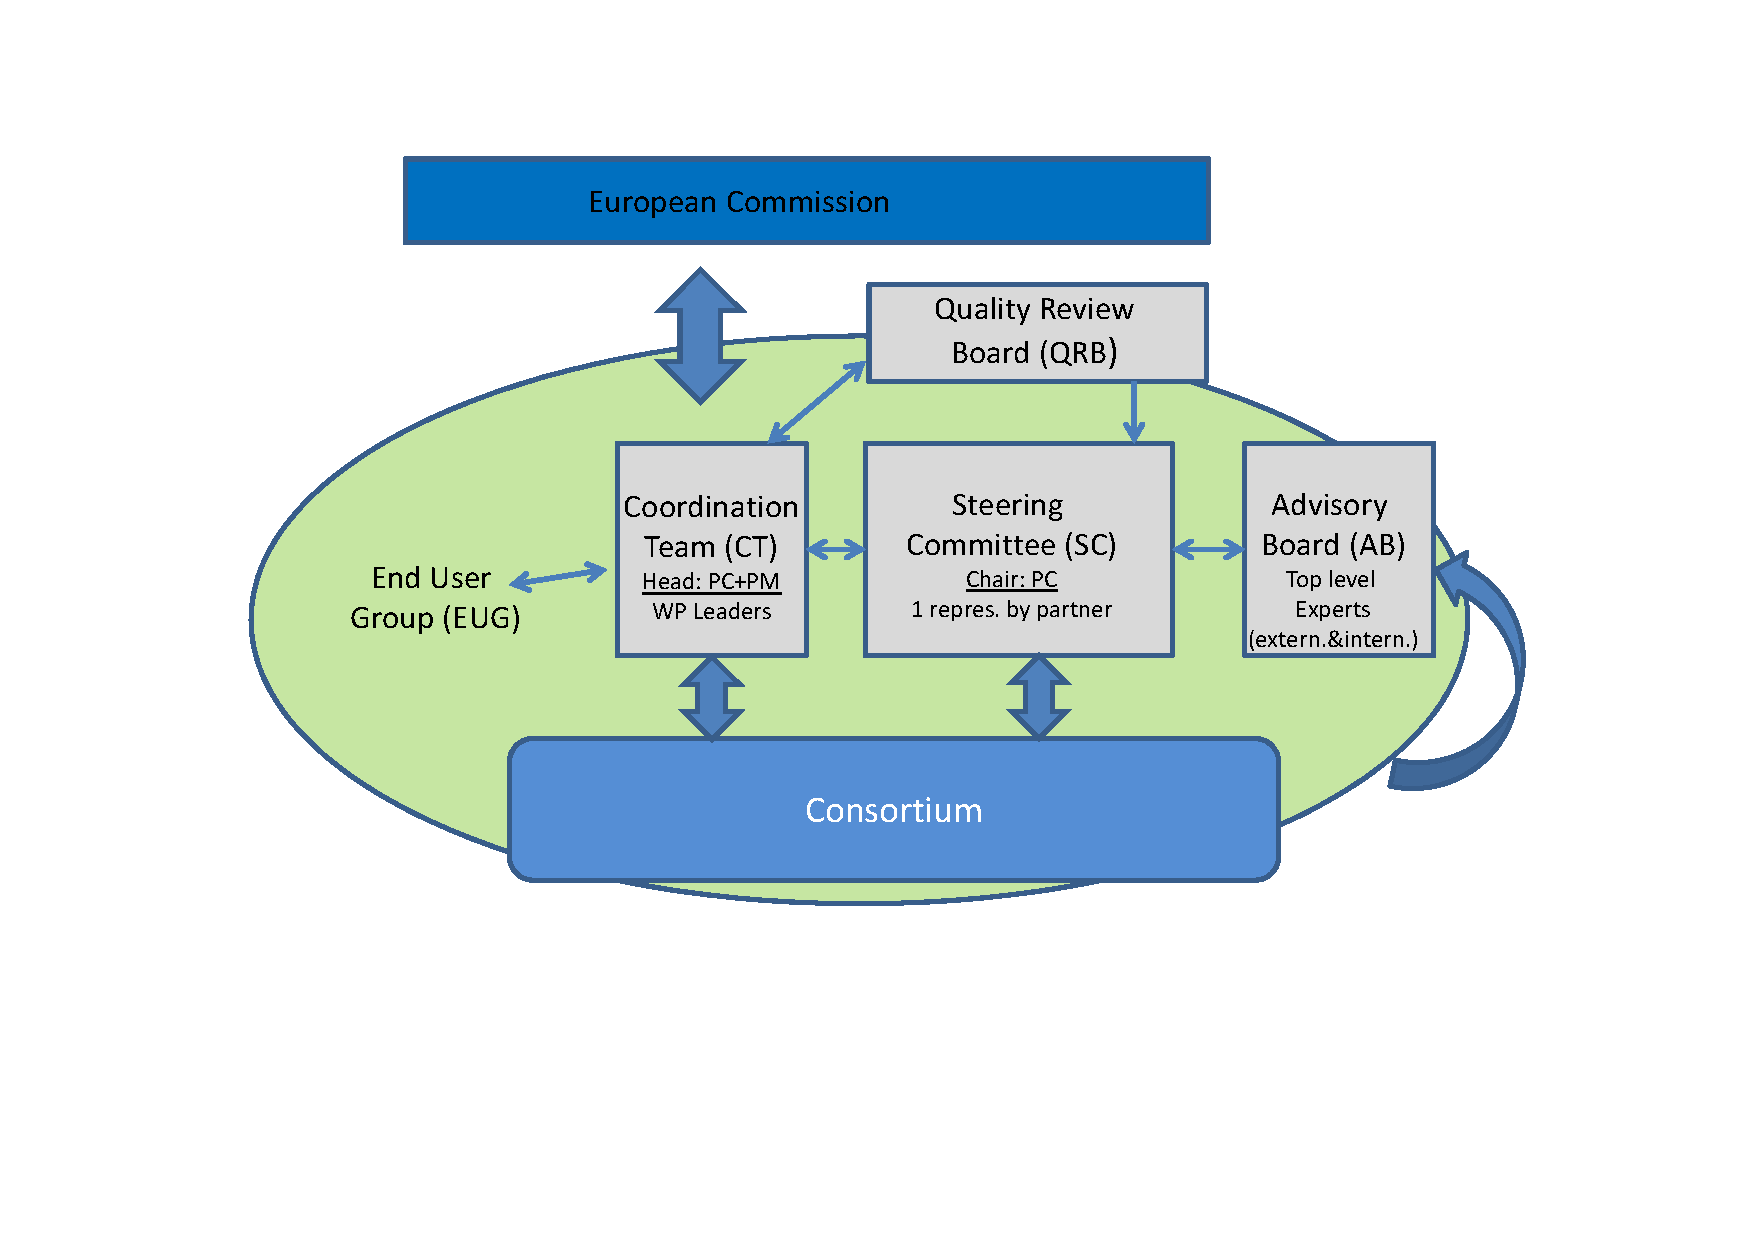
\includegraphics[width=0.75\textwidth]{management_structure.pdf}
  \caption{Management structure}
  \label{figure.management}
\end{figure}

The organizational structure, shown in the Figure~\ref{figure.management}, has been designed
to enable efficient coordination of \TheProject --- the
development and evaluation of a VRE toolkit
integrating several previously separated tools and software and
involving both academic actors and industrial stakeholders.

We have designed the management structure and procedures to deal in a
flexible manner with the following challenges:

\begin{compactitem}
\item to integrate all consortium members and to mobilise their
  expertise, knowledge and networks at every stage of the project;
\item to give the maximum attention to the end-users needs and
  requirements;
\item to continuously involve expertise and knowledge of relevant
  stakeholders and their networks, and
\item to efficiently coordinate the project implementation in a
  collaborative environment and ensure its sustainability.
\end{compactitem}

The coordinator acts as an intermediary between the Partners and
the European Commission. The coordinator will oversee the project
planning, monitor that execution is carried out in time and that
the objectives are achieved and closely interact with the project
officer for project monitoring and delivery of the performance
indicators.  The Project Manager will ensure  efficient day-to-day
management of the project, reporting, feedback to partners on
administrative, financial and legal issues, tracking of  resource
allocation and consumption, and communication inside and outside the
consortium.

The resources of all partners will be mobilised by decentralisation of
responsibilities through the assignment of leadership for work
packages. Clear distribution of tasks, efficient decision making
mechanisms and a sound financial management will safeguard the
achievement of the project’s objectives.

\subsubsection{Project roles}

The following bodies will form the organizational structure of the
\TheProject project : Coordination Team (MT), Steering Committee (SC),
Advisory Board (AB), End User Group (EUG) and Quality Review board
(QRB).

\TOWRITE{NT}{Make this a description}

\noindent\textbf{Coordination Team (CT)}\nobreak\par
\textbf{Members:} The CT is composed of the Work Package leaders
and headed by the Project Coordinator, assisted by the Project
Manager.

\textbf{Responsibilities:} The CT is an executive body in charge of
the project implementation and monitoring.
It takes operational decisions necessary for the smooth execution of
the project.

\textbf{Tasks:}
\begin{compactenum} 
\item Monitoring the timely execution of the tasks and achievement of
  the objectives;
\item Preparation of scientific and financial progress reports;
\item Controlling Work Package progress by assessing it through technical
  reports developed by the partners;
\item Making proposals to the Steering Committee of re-allocation of
  tasks, resources and financial needs for the fulfilment of the work
  plan;
\item Preparing the drafts and validating the project deliverables to
  be submitted to the Commission; 
\end{compactenum} 

\textbf{Meetings:} Project Coordinator and
  Project Manager can meet any time and at least twice a week. They
  will meet Work-Package leaders every 6 months. If necessary,
  extra meetings will be arranged.


\smallbreak\noindent\textbf{Steering Committee (SC)}\nobreak\par

\textbf{Members:} The SC is chaired by the Project Coordinator
and includes one representative from each partner organization.

\textbf{Responsibilities:} The SC is the decision-making body in
charge of the strategic orientation of the project.  It takes decisions on scientific
directions, re-allocation of resources, consortium
changes and intellectual property rights.

\textbf{Meetings:} Every 6 months. If necessary, extra-meetings
will be arranged.  Written minutes of each meeting will be produced,
which shall be the formal record of all decisions taken. A procedure
for comment and acceptance is proposed.

\textbf{Voting procedure:} The SC shall not deliberate until all
Members are present or represented.  Each Member shall have one
vote. The SC will work on consensual decisions as much as possible and
resort to voting only if unavoidable. Voting decisions shall be taken
by a majority of two-thirds (2/3) of votes.

\smallbreak\noindent\textbf{Advisory board (AB)}\nobreak\par

\textbf{Members:} top level experts from partner and external
organizations, including both experts from the project scientific area,
and experts on legal and social matters.

\textbf{Responsibilities:} to give an independent opinion on
scientific and innovation matters, in order to guaranty quality
implementation of the project, efficient innovation management and
project sustainability.  

\textbf{Meetings:} at the request of the Steering Committee.

\textbf{Tentative participants:} The following external persons have
confirmed their interest in being in the advisory board: William
Stein\footnote{\url{wstein.org}} (lead developer of \SMC), one
representative of the Groupe de Travail Logiciel Libre du Pôle de
Compétitivité
Systematic\footnote{\url{http://www.systematic-paris-region.org/en/get-info-topics/free-and-open-source-software}},
Istvan Csabai\footnote{\url{http://complex.elte.hu/~csabai/}} of the
Wigner Research Centre for Physics (WRCP) of the Hungarian Academy of
Sciences.

\smallbreak\noindent\textbf{Quality Review Board (QRB)}\nobreak\par
\textbf{Members:} The QRB will be composed of 2 senior
researchers from the Consortium, 2 representatives of the End User
Group and 2 experts from the Advisory Board. It will be chaired by one
of the professors within the Consortium. All members will be appointed
at the kick-off meeting of the project.  

\textbf{Responsibilities:}
to monitor the quality of the Deliverables, their whole ‘production
process’ and to recommend improvements during the project to the SC.

\textbf{Meetings:} before publications and reports of the
project.

\smallbreak\noindent\textbf{End User Group (EUG)}\nobreak\par

\textbf{Members:} end-users of the VRE, internal and external to
the consortium, from different disciplines and both from academic and
industrial sector. They are actively involved into the project
execution, and work in close interaction with the project coordinator.

\textbf{Responsibilities:} the EUG is the main actor of the innovation
management within the consortium, as they have a deep understanding of
both market and technical problems, and awareness of
opportunities. The EUG also plays a main role in ensuring the VRE
sustainability.  

\textbf{Tasks:} to control the project execution from the
point of view of the end user needs and requirements, to test the tool
and to detect its potential shortcomings at the early stages, to
propose adaptation measures.  

\textbf{Meetings:} the EUG will have regular
virtual meetings, and will meet physically at least once a year.


\subsubsection{Project management tools and procedures}

Project partners and management bodies will communicate through
a dedicated project web platform, maintained by the Project
Manager. WP leaders will monitor progress of
participants of their WP at least monthly, and participants will inform their WP
leaders when problems are encountered. Major problems will be
discussed in (teleconference) meetings with the Project Coordinator
and Project Manager. Each WP leader will be free to organise
extra meetings with WP partners, if necessary. Scientific and
financial progress reports will be collected, assembled and
transmitted to the Project Coordinator by the WP leaders through the
web platform. On basis of the Progress Reports, the Coordination Team
will monitor progress of the project, identify bottlenecks and find
solutions for these problems. Where needed, adaptations to the project
plan will be made, with the aim of ensuring the delivery of the project
results as agreed with the EC. Major adaptations need to be approved
by the Steering Committee.  If necessary, the SC can submit reports to
the QRB for opinion.

Finally, the EUG, working in close cooperation with the
Project Coordinator, will ensure efficient innovation
management. They will carefully monitor new opportunities in
order to give, if necessary, new directions to the project. For
legal aspects, they will have a feedback from legal officers from the
Coordinator’s European Affairs and Technology Transfer office (SAIC),
specialised in Intellectual Property.

Our management structure and procedures will ensure that our network
of 15 partners from both academic and industrial sectors is focused at
achieving the promised deliverables, efficiently managing the
innovation process and largely opening the VRE to its final users. The
15 partners will sign a Consortium Agreement, in which operational
rules and decision making procedures will be laid down. The
international partner will work with a bi-lateral agreement with the
Coordinator.

\subsubsection{Risk management}\label{sec:risks}

The risk in the project execution as planned is carefully assessed and
managed. We base our plans on long standing experience, and we bring
together the world's experts in the relevant tools and techniques.

A key feature of this project is the involvement of a wide set of
partners from multiple domains. While this ensures complementary
coverage of a wide set of skills and provides robustness in different
ways, we will have to ensure that all partners work as closely knit
team. 

Our open source approach means that all our code and outputs
are open and visible to anybody at sites like Github and bitbucket
throughout the project. In particular, it is common for users of
computational software to use the leading edge versions, thus
beta-testing code in-between major releases. This results in risk
reduction: where our design decision or technical approaches are
controversial, this will be detected early by those users, giving the
consortium useful feedback to consider.

The project coordinator will, with support from the Coordination Team
and Quality Review Board, create a Risk Management Plan
\delivref{management}{ipr} as part of the Management Work Package,
which will be reviewed annually. An initial risk assessment appears
as figure \ref{risk-table}.

\begin{figure}
\begin{center}
\begin{tabular}{|m{.2\textwidth}|m{.12\textwidth}|m{.58\textwidth}|}\hline
  Risk & Level with/without mitigation & Mitigation measures\\\hline

  Recruitment of highly qualified staff & High/Medium &
  Great care was taken identifying pool of candidates to hire from,
  and coordinating with currently running projects to rehire personnel
  with strong track record. Typically, we will rehire European
  postdocs that are currently funded by the Sloan grant to work on
  Jupyter in California and wish to come back to Europe.\\\hline

  Different groups not forming effective team & Medium/Low & Long
  track record of working collaboratively on code across multiple
  sites; Aggressive planning of project meetings, work-shops and
  one-to-one partner visits to facilitate most effective teamwork,
  combining face-to-face time at one site with remote
  collaboration.\\\hline 
  % this also justifies our generous travel budget.

  Implementing infrastructure that does not match the needs of end users & High/Low &
  Most of the members of the consortium are themselves end-users with
  a diverse range of needs and points of views; hence the design of
  the proposal and the governance of the project is naturally steered
  by demand; besides, because we provide a toolkit, users have the
  flexibility to adapt the infrastructure to their needs.\\\hline

  Lack of predictability for tasks that are pursued jointly with
  the community & Medium/Low &
  The PI's have a strong experience managing community-developed
  projects where the execution of tasks depends on the availability of
  partners. Some tasks may end up requiring more manpower from
  \TheProject to be completed on time, while others may be entirely
  taken care of by the community. Reallocating tasks and redefining
  work plans is common practice; this anyway happens to cater for a
  fast evolving context. Such random factors will be averaged out over
  the large number of independent tasks.\\\hline
\end{tabular}
\end{center}
\caption{\label{risk-table}Initial Risk Assessment}
\end{figure}
%\TOWRITE{NT/Eugenia}{Impredictability}

%\includegraphics[width=.94\textwidth]{Pictures/Impact-img1.png}

%   But: since Open Source softwares are freely accessible, security
%   and privacy issues are a concern. Anytime a resource is shared,
%   there is greater risk of unauthorised access and contaminated data.
%   Providers must demonstrate security solutions, which should include
%   physical security controlling access to the facility and protection
%   of user data from corruption and cyber attacks.}


%  LocalWords:  mgt Paris-Sud UPSud Thiery Sage-Combinat decentralisation textwidth hline
%  LocalWords:  textwidth Jupyter slmhnlnhfnhs hsfhs ghshsh includegraphics unauthorised

%%% Local Variables:
%%% mode: latex
%%% TeX-master: "proposal"
%%% End:
%  LocalWords:  TOWRITE subsubsection organisational compactenum ipr Impredictability
%  LocalWords:  textbf nobreak smallbreak


\draftpage
\subsection{Consortium as a Whole}
%\TO WRITE{ALL}{Proofread 3.4 consortium pass 2 [Done by Hans]}
%remove this, as we have more pressing things left.

\eucommentary{\begin{compactitem}
\item
Describe the consortium. How will it match the project's objectives?
How do the members complement one another (and cover the value chain,
where appropriate)? In what way does each of them contribute to the
project? How will they be able to work effectively together?
\item
If applicable, describe the industrial/commercial involvement in the
project to ensure exploitation of the results and explain why this is
consistent with and will help to achieve the specific measures which
are proposed for exploitation of the results of the project (see section 2.3).
\item
Other countries: If one or more of the participants requesting EU funding
is based in a country that is not automatically eligible for such funding
(entities from Member States of the EU, from Associated Countries and
from one of the countries in the exhaustive list included in General
Annex A of the work programme are automatically eligible for EU funding),
 explain why the participation of the entity in question is essential to carrying out the project
\end{compactitem}
}

\TOWRITE{All}{Convert site names to standard abbreviations}

The consortium brings together:
\begin{compactenum}
\item \label{mathsoftware} Lead or core developers of a cross-section of the major open
  source computational components for pure mathematics and applications: \GAP (St.~Andrews,
  Oxford), \Linbox (Grenoble), \MPIR (Kaiserslautern), \Pari (CNRS, Versailles), \Sage
  (Orsay, Versailles, CNRS, Oxford, Warwick, Zürich), \Singular (Kaiserslautern).
\item \label{mathdb} Lead developers of a major online mathematical database: \LMFDB
  (Warwick, Zürich).
\item \label{mathknowledge} Experts in mathematical knowledge management (Bremen).
\item \label{smc} The lead developers of the closest thing currently existing to a Virtual
  Research Environment for mathematics: \SMC (Seattle). Because of the key role of \Sage
  in several aspects of the project, and the relevant experience of \SMC as a forerunner of the types
  of systems we want to build, the informal involvement of this US group is adding great value to our project.
  They are keen to provide the benefit of their experience on an unfunded basis, since they wish to remain closely involved in
  all developments in mathematical VREs.
\item \label{jupyter} Experts and major ``promoters'' of the \Jupyter collaborative user
  interfaces for interactive and exploratory computing in a variety of scientific domains
  (Southampton, Simula, Sheffield, Silesia).
\item \label{pythran} Lead developers of the Pythran system for automatic conversion of
  Python to C++ and experts in numerical code optimization/parallelization (\site{LL},
  Grenoble)
\item \label{logilab} A company specialised in open-source based Database and Scientific
  Computing for industry (Logilab); it develops in particular its own virtual environment
  \Simulagora.
\item \label{social} Leading researchers in the sociology of mathematical research and
  collaboration. In particular the coordinating partner of the ``Social Machine of
  Mathematics'' project which has been studying how mathematicians collaborate.
\end{compactenum}





There are many existing points of contact between these groups  and
communities, although many of them are also new to one another. This,
together with the fact that each community is internally collaborative
and part of the broader free software community gives us confidence in
their ability to work together.

\TOWRITE{ALL}{Long track record of collaborations between many of the
  sites. Some of the language below can be used.

Writing interfaces between computer algebra systems from different areas and collaborative
software development are important themes within the DFG Priority Project SPP1489.
As in the {\sc{Sage}} community, networking measures include the regular exchange
of developers and the regular organization of software workshops (coding sprints) which
bring whole teams together for solution finding and intense code writing. Particular tight
collaborations exist between the {\sc{GAP}} and the {\sc{Singular}} communities, with
major {\sc{GAP-Singular}} developers meetings taking alternately place at St~Andrews,
Kaiserslautern, and Aachen. See \url{http://www.computeralgebra.de/}.
}

The exact role of each partner in each work package is defined
in \ref{sec:workpackages}, but in general terms:
\begin{compactitem}
\item Groups \ref{mathsoftware}, \ref{mathdb}, and
\ref{mathknowledge} (from the list above) will collaborate to design the \TheProject VRE
architecture -- the set of interfaces and standards that allow
components to be assembled into bespoke VREs for particular projects
or areas. This architecture will be informed  by the
experience of \ref{logilab} and \ref{smc}; by the sociological
understanding of \ref{social} and from a
\textbf{diverse range of real world use cases from all areas of scientific
  computing, in academia and industry} drawn from their own user bases
and contributed by \ref{logilab} and \ref{smc}.

They will be supported in this work by \ref{smc}, \ref{jupyter} and \ref{pythran} which
bring respectively expertise in the key technologies \SMC and \Jupyter and the Cython
technology.

\item All the participants will make use of the \TheProject VRE, providing feedback to the
  developers and contributing later to the development of demonstrator projects
  (Objective~\ref{objective:demo}). They will also all participate actively in
  dissemination (Objective~\ref{objective:disseminate}) activities.

\item Group \ref{jupyter} will host and mentor core \Jupyter developers to improve this
  key technology (Objective~\ref{objectives:core}), while \ref{mathsoftware},
  \ref{mathdb}, and \ref{mathknowledge} will update their mathematical software components
  (Objective~\ref{objective:updates}) to comply with the newly developed
  interfaces. \ref{pythran} will be a key asset for this work, providing expertise in
  massive parallelism and HPC, bringing in and further developing the specific \Pythran
  optimization technology and providing expertise for development of related technologies
  in other components.  Throughout the consortium, groups have substantial
  experience in open source code development.

\item Group \ref{logilab} will further bring in expertise in semantic databases,
  distribution of large software, and open source based business models.

\item Groups \ref{mathsoftware}, \ref{smc}, and \ref{jupyter} already
  have strong experience in community building and engagement
  (Objective~\ref{objective:community}) for instance through the very
  active user and developer communities around \GAP and \Sage. These
  communities and the dissemination to them of the availability new
  free software constitute the primary exploitation route for this
  project. 
\end{compactitem}

\TOWRITE{ALL}{Add previous collaborations}

%\jointpub{JU,UP,LL,UV}
%\jointproj{UO,USH,UK}
%\jointorga{JU,ZH,SR}
% \jointsoft{PS,UB,UO,UV,ZH,UJF} % Sage development
% \jointsoft{UO,SA} % GAP development
% \jointsoft{UB,UW} % PARI development
% \jointsoft{SR,USH,USO} % IPython; a bit weak
% \jointsoft{PS,LL,WA,ZH} % meeting
% \jointproj{SA,UK} % Science project
% \jointproj{SR,US} % Education project

\coherencetable

%%% Local Variables:
%%% mode: latex
%%% TeX-master: "proposal"
%%% End:


\draftpage

\subsection{Resources to be Committed}
\TOWRITE{ALL}{Proofread 3.4 pass 2 (especially first paragraph Staff efforts)}

\eucommentary{Please provide the following:
\begin{compactitem}
\item
a table showing number of person/months required (table 3.4a)
\item
a table showing 'other direct costs' (table 3.4b) for participants where
those costs exceed 15\% of the personnel costs (according to the budget
table in section 3 of the administrative proposal forms)
\end{compactitem}}

\subsubsection{Management Level Description of Resources and Budget}
\label{sect:budget-details}

\paragraph{Staff efforts}

\eucommentary{Please indicate the number of person/months over the whole
duration of the planned work, for each work package, for each participant.
Identify the work-package leader for each WP by showing the relevant
person-month figure in bold.}

By design \TheProject is attacking upfront the diverse needs of a
very large community: pure maths and applications. Thanks to its
toolkit approach, it will impact users in many areas of science. This
is a major long term investment which requires the extensive expertise
of a large consortium and the improvement of a great number of
software components. The complex technical nature of the project,
combined with the high quality requirements for guaranteeing long term
sustainability, necessitates recruiting highly experienced software
engineers to complement the participants. Much emphasis is put as well
on studying the social aspects and implementing many demonstrators to
illustrate the breath and depth of potential applications.

This all explains the considerable staff efforts%
\ifgrantagreement.\else %
displayed in the following table.
\wpfig[label=fig:staffeffort,caption=Summary of Staff Efforts]
\fi

\paragraph{Travel, dissemination, and outreach}

The community-building nature of this grant proposal requires a large
number of staff exchanges, workshops with project partners, as well as
workshops engaging the wider community in addition to the usual
management and project review meetings. For dissemination, we need to
target the computer science and computational science-focused
communities and their conferences, as well as the domains benefitting
from \TheProject, such as Mathematics and Physical Sciences.

\subparagraph{Guidelines for travel and dissemination}
\label{sect:budget-details-travel}

We use the following guidelines for expected travel expenses:
\euro{2200} for attendance of a typical one week international
conference outside Europe (including travel, subsistence,
accommodation and registration), \euro{1200} for a corresponding
conference in Europe, \euro{750} for a one-week visit of a  project
partner, for instance for coding sprints and one-to-one 
research visits. We expect a similar cost per week while hosting
visitors. For the half-yearly project meetings, we expect on average a
cost of \euro{400} for travel, accommodation and subsistence.

For a partner site with one investigator and one full time researcher,
we expect that that both will attend all of the 9 project meetings that take
place every 6 months (cost of 9 * 2 * 400 =
\euro{7200}), and that the site spends \euro{2000} per year to host
external visitors contributing to the project (total \euro{8000}). We
expect the investigator and the researcher in total to do 4 one-week visits
to other sites (each at \euro{750}) every year, totaling \euro{12000} over 4 years).

% 9*2*400 + 2000*4 + 4*750*4
For dissemination, we expect the researcher to attend on average 1
international conference and 2 European meetings per year (totals
\euro{18400}) and the investigator to attend one international and one
european gathering (totals \euro{13600}).
% (2*2200 + 3*1200)*4

Where there are multiple investigators per site, they will share the
travel and associated costs outlined above. Where there are multiple
researchers, or researchers not employed for the full 48 months, the
travel budget is reduced accordingly.

\subparagraph{Guidelines for outreach costs}
\label{sect:budget-outreach-publication-charges}
We also request \euro{1000} per year per partner (several partners
have other means do pay these costs, and for them these are not needed) 
to pay for open access publication charges.

\label{sect:budget-outreach-workshops}
We request funds for outreach activities such as workshops that
facilitate community building, disseminate best practice and
encourages sustained contributions of the community to the project and
beyond the lifetime of the funding. For  a one-week workshop reaching
out to the community, we cost these at about 400 EUR per participant
to provide accommodation and catering. A workshop for 15 people will
thus cost about \euro{6000}. Participants donate their time and will fund
their own travel. The particular budgeted cost will depend on the
local availability of accommodation and will thus vary from workshop to
workshop. We use creative means to increase value and improve
community building where possible, for example by cooking food
ourselves as done in this recent workshop
\href{http://wiki.sagemath.org/days57}{http://wiki.sagemath.org/days57}.

Details are given in the tables below and in the work packages.

\bigskip

\subsubsection{Resource summaries for consortium member sites}
\label{resources.summary}

%%%%%%%%%%%%%%%%%%%%%%%%%%%%%%%%%%%%%%%%%%%%%%%%%%%%%%%%%%%%%%%%
%
% Guidelines for completion of partner specific resource summary:
%
%
% Please explain how many person months for each person are
% requested. Say who is the local lead. Say anything that helps to
% understand why people are recruited as you plan, in particular if
% this deviates from having one research for 48 months.  We can also
% use this bit of the proposal (and the table, see below) to address
% any other unusual arrangements.
%
%
% The table should contain all non-staff costs (the EU requests that
% this table must be present if the non-staff costs exceed
% 15% of the total cost, but it is good practice and will show
% openness and transparency that we show the data for all partners).
%
% Link back from the table to the work packages and tasks for which
% the expenses are required. Add information that makes it easier to
% understand why the expenses are justified.
%
%     To refer to a task in a work package, use "\taskref{WP-ID}{TASK-ID}" where
%     WP-ID is the ID of the work package:
%        WP#: WP-ID - full title
%        ----------------------
%        WP1: 'management' - Management
%        WP2: 'community' - Community Building and Engagement
%        WP3: 'component-architecture' - Component Architecture
%        WP4: 'UI' - User interfaces
%        WP5: 'hpc' - High Performance Computing
%        WP6: 'dksbases' - Data/Knowledge/Software-Bases
%        WP7: 'social-aspects' - Social Aspects
%        WP8: 'dissem' - Dissemination
%
%
%     and "TASK-ID" is the ID of the task. You can set this using
%
%       \begin{task}[id=TASK-ID,title=Math Search Engine,lead=JU,PM=10,lead=JU]
%
%     To refer to deliverables, use "\delivref{WP-ID}{DELIV-ID}" where DELIV-ID is
%     the ID of the deliverable that can be set like this:
%
%       \begin{wpdeliv}[due=36,id=DELIV-ID,dissem=PU,nature=DEM]
%           {Exploratory support for semantic-aware interactive widgets providing views on objects
%           represented and or in databases}
%       \end{wpdeliv}
%
%
% The table is pre-populated with entries most sites are likely
% to need. If a line does not apply to you, just delete it. If you need
% an extra line, then add it. Use common sense: the number of rows should not
% be very big, but at the same time it is useful to give some breakdown/explanation
% of costs.
%
%
% Eventually, try to create you entry similar in style to the others.
% (The Southampton entry is fully populated, so use this as guidance
% if in doubt.)
%
%
%%%%%%%%%%%%%%%%%%%%%%%%%%%%%%%%%%%%%%%%%%%%%%%%%%%%%%%%%%%%%%%%

In this section we briefly describe the requested resources. See the
participant descriptions in the description of the consortium for the
specific role of each member.

%%%%%%%%%%%%%%%%%%%%%%%%%%%%%%%%%%%%%%%%%%%%%%%%%%%%%%%%%%%%%%%%%%%%%%%%%%%%%%
\paragraph{Resources Université Paris-Sud}

\site{PS} requests 12 person months for the project coordinator
(Nicolas M. Thiéry), 5 person months for two researchers (Florent
Hivert, and Samuel Lelièvre) and for the lead PI (Viviane Pons), 48+36
months for two full time developers, 36 months for a PhD student, and
24 months for a part time project manager for the full duration of the
project.

% 4 * 4k: Developper workshops Cernay
% 6k: Jupyter-Sage
% 2 * 6k: Women in Sage
% Training: 2*4k
% Dissemination CIRM: 16k
% Kickup and final meeting: 2*16k
% workshop: 82k
% (2 * 4 + 3 + 2 * 4 )*(1*2200 + 2*1200) + 2*2000 + 4*750
% travel: 103K


% update table as is appropriate for your contribution. Please remove unused lines.
\bigskip
\begin{table}[H]
\begin{tabular}{|r|r|p{8.5cm}|}
\hline
\textbf{1: \site{PS}} & \textbf{Cost (\euro)} & \textbf{Justification} \\\hline
\textbf{Travel} & 103,000 & Travel (see the guidelines \ref{sect:budget-details-travel})\\\hline
\textbf{Publication charges} & 1,000 & Open access publication charges (see \ref{sect:budget-outreach-publication-charges})\\\hline
%\textbf{Equipment} & ?,??? &  \\\hline    %\taskref{WP-ID}{TASK-ID}
\textbf{Other goods and services} & 92,000 & 8 developer
workshops~\taskref{dissem}{devel-workshops}, 4 training and
dissemination workshops~\taskref{dissem}{dissemination-communication},
audits certificates on the financial statements \\\hline   %\taskref{WP-ID}{TASK-ID} \delivref{WP-ID}{DELIV-ID}
\textbf{Total} & 196,000\\\cline{1-2}
\end{tabular}
\caption{Overview: Non-staff resources to be committed at \site{PS} (all in \texteuro)}\vspace*{-1em}
\end{table}

%%%%%%%%%%%%%%%%%%%%%%%%%%%%%%%%%%%%%%%%%%%%%%%%%%%%%%%%%%%%%%%%%%%%%%%%%%%%%%
\paragraph{Resources CNRS}

CNRS requests 12 person months for the lead PI Vincent Delecroix and
the \PariGP head Karim Belabas, 6 person months for PIs
Bill Allombert and Adrien Boussicault, 5 person months for PI Loïc Gouarin, and
48 person months for a full time developer working on tasks~\taskref{hpc}{hpc-pari},
\taskref{hpc}{hpc-combi}, \taskref{UI}{Sage-display} and \taskref{UI}{pari-python}.

\bigskip
\begin{table}[H]
\begin{tabular}{|r|r|p{8.5cm}|}
\hline
\textbf{2: \site{UB}} & \textbf{Cost (\euro)} & \textbf{Justification} \\\hline
\textbf{Travel}
  &  56,700 & Travel (see the guidelines \ref{sect:budget-details-travel})\\\hline
\textbf{Publication charges}
  &   1,000 & Open access publication charges (see \ref{sect:budget-outreach-publication-charges})\\\hline
%%\textbf{Equipment}
%%  &   0 &  \\\hline    %\taskref{WP-ID}{TASK-ID}
\textbf{Other goods and services}
  & 111,000 &
1 HPC workshop \taskref{dissem}{devel-workshops},
4 Ateliers \Pari \taskref{dissem}{devel-workshops},
4 dissemination workshop in developing countries \taskref{dissem}{dissemination}
 \\\hline   %\taskref{WP-ID}{TASK-ID} \delivref{WP-ID}{DELIV-ID}
\textbf{Total}
 & 168,700\\\cline{1-2}
\end{tabular}
\caption{Overview: Non-staff resources to be committed at \site{CNRS} (all in \texteuro)}\vspace*{-1em}
\end{table}


%%%%%%%%%%%%%%%%%%%%%%%%%%%%%%%%%%%%%%%%%%%%%%%%%%%%%%%%%%%%%%%%%%%%%%%%%%%%%%
\paragraph{Resources Jacobs University Bremen}

\site{JU} requests 6 PM each for the PIs (Prof. Michael Kohlhase leads \WPref{dksbases})
and Dr. habil Florian Rabe (theoretical foundations of triform theories). Furthermore, we
request 24 PM each for a research programmer (Dr. Christian Maeder) and a junior
researcher (Mihnea Iancu M.Sc.). The first will do much of the actually system development
in \WPref{UI} and \WPref{dksbases} while the latter will concentrate on the cases studies
in \WPref{dksbases}.

\bigskip
\begin{table}[H]
\begin{tabular}{|r|r|p{8.5cm}|}
  \hline
  \textbf{3: \site{JU}} & \textbf{Cost (\euro)} & \textbf{Justification} \\\hline
  \textbf{Travel} & 53,600 & Travel (see the guidelines \ref{sect:budget-details-travel})\\\hline
  \textbf{Publication charges} & 4,000 & Open access publication charges (see \ref{sect:budget-outreach-publication-charges})\\\hline
  \textbf{Equipment} & 14,000 &  for two web/compute servers for~\taskref{UI}{mathhub};
   they need 256 GB RAM each for the math search engine from~\taskref{dksbases}{mws}\\\hline
\textbf{Other goods and services} & 4,300 & Audits certificates on the financial statements \\\hline
\textbf{Total} & 75,900\\\cline{1-2}
\end{tabular}
\caption{Overview: Non-staff resources to be committed at \site{JU} (all in \texteuro)}\vspace*{-1em}
\end{table}

%%%%%%%%%%%%%%%%%%%%%%%%%%%%%%%%%%%%%%%%%%%%%%%%%%%%%%%%%%%%%%%%%%%%%%%%%%%%%%
\paragraph{Resources Universit\'{e} Joseph Fourier}

% See guidance above ("Guidelines for completion of partner specific resource summary") for what to add here.
UJF requests 12 person months for an engineer (Pierrick Brunet) starting in
month 0 and working on \taskref{hpc}{pythran}, 24 person
months for another engineer starting in month 12 and working on \taskref{hpc}{hpc-linbox}, 15 person months for the lead PI
(Clément Pernet) and 9 person months for a PI (Jean-Guillaume Dumas).
The lead PI will take on all management responsibilities. The
engineers will not be employed for the whole project duration, and
the PIs will carry out all tasks for the project in the remaining
period.

% update table as is appropriate for your contribution. Please remove unused lines.
\bigskip
\begin{table}[H]
\begin{tabular}{|r|r|p{8.5cm}|}
\hline
\textbf{4: \site{UJF}} & \textbf{Cost (\euro)} & \textbf{Justification} \\\hline
\textbf{Travel} & 60,850 & Travel (see the guidelines \ref{sect:budget-details-travel})\\\hline
\textbf{Publication charges} & 1,000 & Open access publication charges (see \ref{sect:budget-outreach-publication-charges})\\\hline
\textbf{Equipment} & 24,000 &A large multicore server with
multiple accelerators to experiment heterogeneous computing; 2 laptops  \\\hline     %\taskref{WP-ID}{TASK-ID}

\textbf{Other goods and services} & 34,000 & 2 developer workshops: HPC and Pythran,
audits certificates on the financial statements \\\hline   %\taskref{WP-ID}{TASK-ID} \delivref{WP-ID}{DELIV-ID}
\textbf{Total} & 119,850\\\cline{1-2}
\end{tabular}
\caption{Overview: Non-staff resources to be committed at \site{UJF} (all in \texteuro)}\vspace*{-1em}
\end{table}


%%%%%%%%%%%%%%%%%%%%%%%%%%%%%%%%%%%%%%%%%%%%%%%%%%%%%%%%%%%%%%%%%%%%%%%%%%%%%%
\paragraph{Resources University of Kaiserslautern}


% See guidance above ("Guidelines for completion of partner specific resource summary") for what to add here.

\site{UK} requests 48 person months for a researcher to work on
tasks~\taskref{hpc}{hpc-singular} (46 PM), \taskref{UI}{ipython-kernels} (2 PM), 12
person months for a researcher starting in month 6 to work on
\taskref{hpc}{hpc-mpir}. The cost for Professor Decker's
activities within OpenDreamKit (6 PM), including the related overhead,
will be covered by \site{UK} and is therefore not part of the requested
funding. The lead PI will take on all management responsibilities.


% update table as is appropriate for your contribution. Please remove unused lines.
\bigskip
\begin{table}[H]
\begin{tabular}{|r|r|p{8.5cm}|}
\hline
\textbf{5: \site{UK}} & \textbf{Cost (\euro)} & \textbf{Justification} \\\hline
\textbf{Travel} & 67,100 & Travel (see the guidelines \ref{sect:budget-details-travel})\\\hline
\textbf{Other goods and services} & 67,600 &
  5 developer workshops~\taskref{dissem}{devel-workshops},
  audits certificates on the financial statements \\\hline
\textbf{Total} & 134,700\\\cline{1-2}
\end{tabular}
\caption{Overview: Non-staff resources to be committed at \site{UK} (all in \texteuro)}\vspace*{-1em}
\end{table}

%%%%%%%%%%%%%%%%%%%%%%%%%%%%%%%%%%%%%%%%%%%%%%%%%%%%%%%%%%%%%%%%%%%%%%%%%%%%%%
\paragraph{Resources University of Oxford}

University of Oxford requests 24 person months for a co investigator (Dmitrii Pasechnik),
who will be employed for the whole duration of the project, 2 person months for the
lead PI (Ursula Matrin) and 3 person months for the other co investigator (Edith Elkind) to
work on WP7, of which 2 person months for WP1 (Management).
From his total involvement, Pasechnik will take 4 person months to work on WP3.
Martin and Elkind both hold personal fellowships (funded by EPSRC (UK) and by ERC, respectively)
on topics closely related to the project, enabling them to take part 
in the project only at a fraction of the full cost; however, 
they will need funding to travel to project meetings.
Open access publication charges will be met by the host institution.

\bigskip
\begin{table}[H]
\begin{tabular}{|r|r|p{8.5cm}|}
\hline
\textbf{6: \site{UO}} & \textbf{Cost (\euro)} & \textbf{Justification} \\\hline
\textbf{Travel} & 25,000 & Travel (see the guidelines \ref{sect:budget-details-travel})\\\hline
\textbf{Equipment} & 3,000 & Laptop and a large display for a co investigator \\\hline    %\taskref{WP-ID}{TASK-ID}

\textbf{Total} & 28,000\\\cline{1-2}
\end{tabular}
\caption{Overview: Non-staff resources to be committed at \site{UO} (all in \texteuro)}\vspace*{-1em}
\end{table}

%%%%%%%%%%%%%%%%%%%%%%%%%%%%%%%%%%%%%%%%%%%%%%%%%%%%%%%%%%%%%%%%%%%%%%%%%%%%%%
\paragraph{Resources University of Silesia}

University of Silesia will include three people in the project and
their involvement will 12 person months each. Jerzy Luczka and Jan Aksamit will
work on interactive books \taskref{dissem}{ibook} which will
demonstrate the real case of using both Structured Text and
interactive features of the VRE. Marcin Kostur will lead and
contribute to this task as well.

Marcin Kostur will lead the part of \taskref{UI}{cfd-vis} which will
be connected with 3d visualisation of data produced by the Lattice
Boltzmann software 'sailfish'. After initial research work done
together with Simula (task leader) will require to subcontract the
development of software visualisation.

The justification for subcontracting is as follows. We have much
experience as users of 3d visualisation software for fluid
dynamics. However the expertise in Computer Graphics (e.g. WebGL) is
not enough at the Department of Mathematics, Physics and
Chemistry. Instead of building the expertise it is financially more
efficient to specify and outsource the programming task to professionals.

% travel (4*2200+5*750+5*400)*1.25

\bigskip
\begin{table}[H]
\begin{tabular}{|r|r|p{8.5cm}|}
\hline
\textbf{7: \site{US}} & \textbf{Cost (\euro)} & \textbf{Justification} \\\hline
\textbf{Travel} & 18,188 & Travel (see the guidelines \ref{sect:budget-details-travel})\\\hline
%\textbf{Publication charges} & 0,000 & Open access publication charges (see \ref{sect:budget-outreach-publication-charges})\\\hline
%\textbf{Other goods and services} & 50,000 & Subcontracting costs  \\\hline   %\taskref{WP-ID}{TASK-ID} \delivref{WP-ID}{DELIV-ID}
\textbf{Total} & 18,188\\\cline{1-2}
\end{tabular}
\caption{Overview: Non-staff resources to be committed at \site{US} (all in \texteuro)}\vspace*{-1em}
\end{table}

%%%%%%%%%%%%%%%%%%%%%%%%%%%%%%%%%%%%%%%%%%%%%%%%%%%%%%%%%%%%%%%%%%%%%%%%%%%%%%
\paragraph{Resources University of Sheffield}

Sheffield requests 42 person months for a researcher, 6 person months
for the lead PI (Neil Lawrence) and 6 person months for the
co-Investigator (Mike Croucher). The lead PI will take on all
management responsibilities. Two researchers will be employed, one for
a shorter period of 6 months, with a specific focus on the SGE
Implementation \taskref{hpc}{hpc-jupyter}. The other for a period of
36 months, with appointment at month 6, whose focus will be on user
interfaces, social aspects \taskref{social-aspects}{social-output} and
course development \taskref{dissem}{project-intro}.  researcher will
not be employed for the whole project duration, and the PIs will carry
out all tasks for the project in the remaining period. One person
month of an administrator is requested for assistance with workshop
and meeting organisation etc.

Sheffield will host one of the project main workshops (15,000) and will also host two
workshops on machine learning and data science with \TheProject. We also request equipment
for workshop recording at 2,000, and funding for a large touch screen for live notebook
posters (\delivref{social-aspects}{social-poster}) at 5,000. For the researchers we
request screens and computers (3,000).
% See guidance above ("Guidelines for completion of partner specific resource summary") for what to add here.

% Travel costs computation: project meetings + external hosting + site visits + conference travel
% 9*2*400 + 2000*4 + 4*750*2 + (2*2200 + 3*1200)*4

% update table as is appropriate for your contribution. Please remove unused lines.
\bigskip
\begin{table}[H]
\begin{tabular}{|r|r|p{8.5cm}|}
\hline
\textbf{8: \site{USH}} & \textbf{Cost (\euro)} & \textbf{Justification} \\\hline
\textbf{Travel} & 53,200 & Travel (see the guidelines \ref{sect:budget-details-travel})\\\hline
\textbf{Publication charges} & 4,000 & Open access publication charges (see \ref{sect:budget-outreach-publication-charges})\\\hline
\textbf{Equipment} & 10,000 & High performance laptops and multi touch large screen for \taskref{social-aspects}{social-output} \\\hline

\textbf{Other goods and services} & 28,000 & Workshops (Project meeting and two dissemination workshops, see \taskref{dissem}{project-intro}),
  HPC Compute Time (see \taskref{hpc}{hpc-jupyter}),
  audits certificates on the financial statements \\\hline
\textbf{Total} & 95,200 \\\cline{1-2}
\end{tabular}
\caption{Overview: Non-staff resources to be committed at \site{USH} (all in \texteuro)}\vspace*{-1em}
\end{table}

%%%%%%%%%%%%%%%%%%%%%%%%%%%%%%%%%%%%%%%%%%%%%%%%%%%%%%%%%%%%%%%%%%%%%%%%%%%%%%
\paragraph{Resources Southampton}

Southampton requests 38 person months for a researcher (expected to
start in month 4 of the project), 6 person months for the lead PI
(Hans Fangohr) and 2 person months for the co investigator (Ian
Hawke). The lead PI will take on all management responsibilities. The
researcher will not be employed for the whole project duration, and
the PIs will carry out all tasks for the project in the remaining
period.

\bigskip
\begin{table}[H]
\begin{tabular}{|r|r|p{8.5cm}|}
\hline
\textbf{9: \site{USO}} & \textbf{Cost (\euro)} & \textbf{Justification} \\\hline
\textbf{Travel} & 51,500& Travel (see the guidelines \ref{sect:budget-details-travel})\\\hline
\textbf{Publication charges} & 4,000 & Open access publication charges (see \ref{sect:budget-outreach-publication-charges})\\\hline
\textbf{Equipment} & 10,000 & HPC Workstation (6k) to host
micromagnetic VRE web server, \taskref{UI}{oommf-nb-ve}, and two high performance laptops (2x2k)\\\hline
\textbf{Other goods and services} & 24,800 &
  4 Dissemination workshops overseas (travel for teachers \& room hire),
  \taskref{dissem}{dissemination-of-oommf-nb-workshops},
  audits certificates on the financial statements\\\hline
\textbf{Total} & 86,300\\\cline{1-2}
\end{tabular}
\caption{Overview: Non-staff resources to be committed at \site{USO} (all in \texteuro)}\label{tab:resources-non-staff-southampton}\vspace*{-1em}
\end{table}

%%%%%%%%%%%%%%%%%%%%%%%%%%%%%%%%%%%%%%%%%%%%%%%%%%%%%%%%%%%%%%%%%%%%%%%%%%%%%%
\paragraph{Resources University of St Andrews}

St Andrews requests 9.6 person months for the lead PI
(Steve Linton), 24 person months for the co-investigator
(Alexander Konovalov) and 48 person months for the 
researcher (Markus Pfeiffer). The lead PI will take on all 
management responsibilities.

\bigskip
\begin{table}[H]
\begin{tabular}{|r|r|p{8.5cm}|}
\hline
\textbf{10: \site{SA}} & \textbf{Cost (\euro)} & \textbf{Justification} \\\hline
\textbf{Travel} & 76,800 & Travel (see the guidelines \ref{sect:budget-details-travel})\\\hline
\textbf{Publication charges} & 4,000 & Open access publication charges (see \ref{sect:budget-outreach-publication-charges})\\\hline
\textbf{Equipment} & 15,000 & Compute servers for parallel software development and testing
(tasks \taskref{hpc}{hpc-gap}, \taskref{component-architecture}{component-for-HPC}) \\\hline

\textbf{Other goods and services} & 21,500 &
  2 dissemination workshops (room hire and subsistence for external participants; task \taskref{dissem}{devel-workshops}),
  audits certificates on the financial statements
 \\\hline
\textbf{Total} & 117,300\\\cline{1-2}
\end{tabular}
\caption{Overview: Non-staff resources to be committed at \site{SA} (all in \texteuro)}\vspace*{-1em}
\end{table}


%%%%%%%%%%%%%%%%%%%%%%%%%%%%%%%%%%%%%%%%%%%%%%%%%%%%%%%%%%%%%%%%%%%%%%%%%%%%%%
\paragraph{Resources Universit\'{e} de Versailles Saint-Quentin}

Universit\'{e} de Versailles Saint-Quentin requests 12 person months
for the lead PI (Luca De Feo) and 2 person months for a researcher
(Nicolas Gama). Because of its small size and geographical proximity
to \site{PS}, Universit\'{e} de Versailles is not going to hire any
full-time personnel for the project.

\bigskip
\begin{table}[H]
\begin{tabular}{|r|r|p{8.5cm}|}
\hline
\textbf{11: \site{UV}} & \textbf{Cost (\euro)} & \textbf{Justification} \\\hline
\textbf{Travel} & 12,600 & Travel (4 EU conferences, 4 one week visits to project partners, 12 project meetings)\\\hline
\textbf{Total} & 12,600\\\cline{1-2}
\end{tabular}
\caption{Overview: Non-staff resources to be committed at \site{UV} (all in \texteuro)}\vspace*{-1em}
\end{table}

%%%%%%%%%%%%%%%%%%%%%%%%%%%%%%%%%%%%%%%%%%%%%%%%%%%%%%%%%%%%%%%%%%%%%%%%%%%%%%
\paragraph{Resources University of Warwick}

Warwick requests 24 person months for a researcher expected to start
around month 6 of the project to work on WP6, and 3 person months for
the lead PI (John Cremona) for WP1 (Management) and WP6. The
researcher will not be employed for the whole project duration, and
the PI will carry out any remaining tasks for the project.  The PI,
who is also PI on the LMFDB grant, will be able to use alternative
funding for conference attendance, and only requires travel support
for project meetings and visiting other sites.  The workshop to be
hosted will be joint with the LMFDB project and part-funded by the
LMFDB grant.  Open access publication charges will be met by the host
institution.

% update table as is appropriate for your contribution. Please remove unused lines.
\bigskip
\begin{table}[H]
\begin{tabular}{|r|r|p{8.5cm}|}
\hline
\textbf{12: \site{UW}} & \textbf{Cost (\euro)} & \textbf{Justification} \\\hline
\textbf{Travel} & 9,600 & Project meetings and partner site visits;
investigator co-funded by LMFDB grant (see \ref{sect:budget-details-travel})\\\hline
\textbf{Equipment} & 4,000 & laptops for investigator and researcher\\\hline    %\taskref{WP-ID}{TASK-ID}

\textbf{Other goods and services} & 12,000 & Hosting one workshop
co-funded by LMFDB project\\\hline   %\taskref{WP-ID}{TASK-ID} \delivref{WP-ID}{DELIV-ID}
\textbf{Total} & 25,600\\\cline{1-2}
\end{tabular}
\caption{Overview: Non-staff resources to be committed at \site{UW} (all in \texteuro)}\vspace*{-1em}
\end{table}

%%%%%%%%%%%%%%%%%%%%%%%%%%%%%%%%%%%%%%%%%%%%%%%%%%%%%%%%%%%%%%%%%%%%%%%%%%%%%%
\paragraph{Resources University of Z\"{u}rich}
Zurich will employ one person associated with the project, Paul-Olivier Dehaye. Twelve person-months will be dedicated to \WPref{dksbases} and spread over the four years, with an extra one for the management (\WPref{management}). He will devote additional time to these efforts, paid from other sources (University of Zurich and Swiss Science Foundation).

He will lead tasks \taskref{dksbases}{data-assessment}, and assist for
\taskref{dksbases}{data-design}, \taskref{dksbases}{data-triform},
\taskref{dksbases}{data-foundationCAS}, \taskref{dksbases}{data-findstat} and
\taskref{dksbases}{data-LMFDB}. He is in charge of deliverables \delivref{dksbases}{conv},
and \delivref{dksbases}{lfmverif}.

\bigskip
\begin{table}[H]
\begin{tabular}{|r|r|p{8.5cm}|}
\hline
\textbf{13: \site{ZH}} & \textbf{Cost (\euro)} & \textbf{Justification} \\\hline
\textbf{Travel} & 26,800 & Travel (see the guidelines \ref{sect:budget-details-travel})\\\hline
\textbf{Publication charges} & 4,000 & Open access publication charges (see \ref{sect:budget-outreach-publication-charges})\\\hline
\textbf{Equipment} & 2,000 &  laptop for investigator \\\hline    %\taskref{WP-ID}{TASK-ID}

%\textbf{Other goods and services} & ?,??? & Workshops \\\hline   %\taskref{WP-ID}{TASK-ID} \delivref{WP-ID}{DELIV-ID}
\textbf{Total} & 32,800\\\cline{1-2}
\end{tabular}
\caption{Overview: Non-staff resources to be committed at \site{ZH} (all in \texteuro)}\vspace*{-1em}
\end{table}


%%%%%%%%%%%%%%%%%%%%%%%%%%%%%%%%%%%%%%%%%%%%%%%%%%%%%%%%%%%%%%%%%%%%%%%%%%%%%%
\paragraph{Resources Logilab}

Logilab requests 36 person months for its engineers (Julien Cristau,
Florent Cayré and Olivier Cayrol). They will bring their expertise
(database design, software architecture, computer-domain knowledge) to
numerous tasks, and will notably contribute to the packaging of \Sage
(\taskref{component-architecture}{mod-packaging}), the enhancement of
existing forges (\taskref{component-architecture}{workflow}) and the
addition of HTML5 widgets in notebooks
(\taskref{UI}{dynamic-inspect}).

Logilab requests 12 person months for subcontracting an engineer
(Serge Guelton), main developer of \Pythran, that will work on
\taskref{hpc}{pythran}.

% Travels: 1 conference extra-EU, 4 conferences EU, 9 project meetings for 2 persons, 4 workshops
% 1*2200 + 4*1200 + 2*2000 + (9*2)*400 + 4*750 = 17,200


\bigskip
\begin{table}[H]
\begin{tabular}{|r|r|p{8.5cm}|}
\hline
\textbf{14: \site{LL}} & \textbf{Cost (\euro)} & \textbf{Justification} \\\hline
\textbf{Travel} & 17,200 & Travel (see the guidelines \ref{sect:budget-details-travel})\\\hline
\textbf{Total} & 17,200\\\cline{1-2}
\end{tabular}
\caption{Overview: Non-staff resources to be committed at \site{Logilab} (all in \texteuro)}\vspace*{-1em}
\end{table}

%%%%%%%%%%%%%%%%%%%%%%%%%%%%%%%%%%%%%%%%%%%%%%%%%%%%%%%%%%%%%%%%%%%%%%%%%%%%%%
\paragraph{Simula Research Laboratory}

Simula requests 28 person months for research activities to lead Work package 4 and contribute to its specific tasks. 
We also dedicate 4 person months for management  as well as  dissemination and communication activities (to be split equally). These activities will be mainly performed by the lead PI with the extensive support of the local management team.  
% update table as is appropriate for your contribution. Please remove unused lines.
\bigskip
\begin{table}[H]
\begin{tabular}{|r|r|p{8.5cm}|}
\hline
\textbf{15: \site{SR}} & \textbf{Cost (\euro)} & \textbf{Justification} \\\hline
\textbf{Travel} & 56,200 & Travel (see the guidelines \ref{sect:budget-details-travel})\\\hline
\textbf{Publication charges} & 4,000 & Open access publication charges (see \ref{sect:budget-outreach-publication-charges})\\\hline
%\textbf{Equipment} & 0 &  \\\hline    %\taskref{WP-ID}{TASK-ID}

\textbf{Other goods and services} & 11,500 &
   Organisation of the Jupyter workshop,
   audits certificates on the financial statements
   \\\hline   %\taskref{WP-ID}{TASK-ID} \delivref{WP-ID}{DELIV-ID}
\textbf{Total} & 71,700\\\cline{1-2}
\end{tabular}
\caption{Overview: Non-staff resources to be committed at \site{Simula} (all in \texteuro)}\vspace*{-1em}
\end{table}

% \subsubsection{Resources Summary}

% \begin{table}[ht]\centering
%   \TODO{Table 3.4.a: insert here table from Figure 3, and transpose; see
%     Table 3.4.a in the word template}
%   \TODO{The work package leader will usually have the largest investment}
%   \TODO{This table is in the wrong place in the proposal - before work packages, not after}
% \caption{Overview: Resources to be committed (all in \texteuro)}\label{tab:resources}\vspace*{-1em}
% \end{table}
% \fbox{\begin{minipage}{\textwidth}

% \eucommentary{Please complete the table below for each participant if the sum of the costs for’ travel’, ‘equipment’,
% and ‘goods and services’ exceeds 15% of the personnel costs for that participant (according to the
% budget table in section 3 of the proposal administrative forms).}

% \begin{center}\Large\bf
% Other direct cost items
% \end{center}
% \end{minipage}}

% \bigskip

% \begin{tabular}{|r|l|p{8.5cm}|}
% \hline
% \textbf{\TheProject} & \textbf{Cost (\euro)} & \textbf{Justification} \\\hline
% \textbf{Travel} & & \\\hline
% \textbf{Equipment} & & \\\hline
% \textbf{Other goods and services} & & \\\hline
% \textbf{Total} & \\\cline{1-2}
% \end{tabular}




%%% Local Variables:
%%% mode: latex
%%% TeX-master: "proposal"
%%% End:

%  LocalWords:  newpage fbox minipage textwidth eucommentary bigskip rr rr rr hline hpc
%  LocalWords:  vspace texteuro textbf textbf textbf TOWRITE subsubsection taskref dissem
%  LocalWords:  dksbases delivref wpdeliv Universit Sud Logilab Fangohr OOMMFNB JacU Feo
%  LocalWords:  oommf-nb-ve dissemination-of-oommf-nb-workshops Simula Laboratory Thiéry
%  LocalWords:  Hivert Lelièvre Developper Cernay Jupyter-Sage Kickup devel-workshops mws
%  LocalWords:  Gama Pierrick pythran hpc-linbox Pernet Delecroix Belabas Allombert Loic
%  LocalWords:  Boussicault Gouarin hpc-combi Dmitrii Pasechnik Matrin Elkind hpc-jupyter
%  LocalWords:  Konovalov mathhub Luczka Aksamit Kostur cfd-vis Dehaye WPref WPref conv
%  LocalWords:  data-findstat lmfmod lmfval Organisation Jupyter habil Maeder Mihnea mpir
%  LocalWords:  Iancu localtaskref ipython-kernels Cristau Cayré Cayrol Guelton wpfig
%  LocalWords:  micromagnetic staffeffort


% ---------------------------------------------------------------------------
%  Section 4: Members of the Consortium
% ---------------------------------------------------------------------------

\newpage

\eucommentary{This section is not covered by the page limit.\\
The information provided here will be used to judge the operational capacity.}

\section{Members of the Consortium}

\TOWRITE{ALL}{Proofread 4. Members of the consortium pass 2}

\subsection{Participants}

\eucommentary{Please provide, for each participant, the following (if available):\\
\begin{compactitem}
\item
a description of the legal entity and its main tasks,
with an explanation of how its profile matches the tasks in the proposal;
\item
a curriculum vitae or description of the profile of the persons,
including their gender, who will be primarily responsible for carrying
out the proposed research and/or innovation activities;
%
this includes a description of the profile of the to-be-recruited personnel
\item
a list of up to 5 relevant publications, and/or products, services
(including widely-used datasets or software), or other achievements
relevant to the call content;
\item
a list of up to 5 relevant previous projects or activities, connected
to the subject of this proposal;
\item
a description of any significant infrastructure and/or any major items
of technical equipment, relevant to the proposed work;
\item
any other supporting documents specified in the work programme for this call.
\end{compactitem}}

\begin{sitedescription}{PS}

University Paris-Sud is among the 40 top universities worldwide in the
2013 Shanghai ranking, and is one of the two best French research
universities. With about 27000 students, 1800 permanent teaching staff
and 1300 permanent research scientists from national research
organisations (CNRS, Inserm, INRA, Inria), it is the largest campus in
France. Since 2006, scientists from the University were awarded two
Fields medals, one Nobel Prize and a number of other international
(European Inventor Award 2013, Wolf Prize 2010, Holweck Prize 2009,
Japan prize 2007) and national prizes.  The Université Paris-Sud has a
complete array of competences, ranging from the purest of exact
sciences to clinical practices in medicine, covering life and health
sciences, legal sciences and economics. Research at the Université
Paris-Sud, an essential part of academic understanding, is
complemented by research activities with a high valorisation
potential. Research contracts and partnership with companies make the
Université Paris-Sud a key actor and a major player in French
research.  The University is located close to the Plateau de Saclay,
the largest cluster of public and private R\&D institutions in France
(with ca. 16000 research staff), and is one of the core members of the
University Paris Saclay – a world class university and a
world-renowned research and innovation hub.

In the context of this project, the Université Paris Saclay is the
home of one of the largest group of Sage developers worldwide. It's a
member of the Open Source Thematic Group of the Systematic Paris
Region Systems and ICT Cluster. The University also hosts a major
research group working on proof assistants (Coq), which naturally
opens the door for reaching toward this neighbor community.

% The main participants have accumulated 15 years of experience of
% collaborative open source software development for mathematics
% leadership, and community animation.

\subsubsection*{Curriculum vitae of the investigators}

\begin{participant}[type=leadPI,PM=6,salary=4200,gender=female]{Viviane Pons}
  Maître de Conférences at the Laboratoire de Recherche en Informatique, Viviane Pons is a
  young researcher in Algebraic Combinatorics. She defended her thesis in 2013 and has 3
  papers in international journals and 3 communications in international
  conferences, including a talk at PyCon US 2015. Before starting research career, 
  she worked for two years in industry as a Java and web developer.

  She discovered \Sage during her first \Sage Days in 2010 and has since been an active user
  and contributor with 10 (co)authored tickets improving the support of combinatorial
  objects in \Sage. She is heavily involved in the promotion of \Sage, participating in
  \Sage Days and running \Sage introduction tutorials or \Sage presentations at various
  conferences. She is also one of the main developers of the project \software{FindStat}
  dedicated to databases in combinatorics.
\end{participant}
%%% Local Variables:
%%% mode: latex
%%% TeX-master: "../proposal"
%%% End:

%\input{CVs/Nathann.Cohen}
\begin{participant}[type=PI,PM=6,salary=9000,gender=male]{Florent Hivert}

  Professor at the Laboratoire de Recherche en Informatique, Florent Hivert is a senior
  researcher in Algebraic Combinatorics with 29 papers in international journals and 15
  communications in international conferences.
% including an invited lecture at FPSAC'10

With 100 \Sage tickets (co)authored and as many refereed, Hivert is himself a core \Sage
developer, with contributions including key components of the \Sage infrastructure
(documentation, automated test, combinatorics infrastructure, parallelism, \ldots)
and specialised research libraries.
\end{participant}
%%% Local Variables:
%%% mode: latex
%%% TeX-master: "../proposal"
%%% End:

\paragraph{Nicolas M. Thiéry}

Professor at the Laboratoire de Recherche en Informatique, Nicolas
M. Thiéry is a senior researcher in Algebraic Combinatorics with an
international recognition. Among other things, he is a member of the
permanent committee of FPSAC, the main international conference of the
domain, and has collaborators in Canada, India, and in the US where he
spent several years; he also coorganized many international workshops,
in particular Sage Days, and a semester long program hosted by ICERM.

Algebraic combinatorics is a field at the frontier between mathematics
and computer science, with heavy needs for computer
exploration. Pioneer in community-developed open source software for
research in this field, Thiéry founded in 2000 the Sage-Combinat
software project; with 50 researchers in Europe and abroad, this
project has grown under his leadership to be one of the largest
organized community of Sage developers, gaining a leading position in
its field, and making a major impact on one hundred publications. At
this occasion, Thiéry gained a strong community building experience,
and coauthored some of NSF Sage-Combinat grant OCI-1147247.

With 150 tickets (co)authored and as many refereed, Thiéry is himself
a core Sage developer, with contributions including key components of
the Sage infrastructure (e.g. categories), specialized research
libraries (e.g. root systems), thematic tutorials, and two chapters of
the book ``Calcul Mathématique avec Sage''.

\begin{participant}[type=R,PM=6,gender=male]{Samuel Lelièvre}

Maître de conférences since 2006 at
Laboratoire de mathématique d'Orsay, Université Paris-Sud,
% PhD Rennes 2004 under Anton Zorich,
% post-doc Warwick with Vladimir Markovic,
Samuel Lelièvre is an established researcher in Dynamics and Geometry,
with 10 papers published in international journals including
Annales scientifiques de l'École normale supérieure,
Crelle, GAFA, Geometry and Topology.
He participated in three ANR projects, and has collaborators
in France, Israel, the UK, the USA.
His research in Dynamics and Geometry
often involves explicit and experimental approaches,
for which he writes code in order to explore
combinatorial objects such as square-tiled surfaces,
translation surfaces, group actions, group presentations.

He uses and actively promotes Sage since 2010.
He is in the top 15 contributors of the Ask-Sage
questions and answers site.
He coorganized six international meetings including two Sage Days,
presented Sage at PyCon-FR-2011 in Rennes,
supervised Sage tutorials twice at the GDR-IM yearly school
for French PhD students at the interface of Mathematics and
Computer Science, and at the CIMPA/ICPAM school Bobo2012
on Discrete Mathematics (Bobo Dioulasso, Burkina Faso, 2012).
\end{participant}
%%% Local Variables:
%%% mode: latex
%%% TeX-master: "../proposal"
%%% End:

\begin{participant}[type=R,PM=6,gender=male,salary=5600]{Lo\"ic Gouarin}
  Research Engineer since 2005 at CNRS and more specifically since
  2010 at the Laboratoire de Mathématique d'Orsay, Université
  Paris-Sud, Loïc Gouarin develops scientific computing software in
  different fields like Lattice-Boltzmann methods, Stokes solvers for
  fluid particles interaction, ...

  He is also director of the ``GdR Calcul'' and co-director of the
  ``Réseau Calcul''. These two entities form the ``Groupe Calcul'' of
  the CNRS whose role is to animate the scientific and high
  performance computing community in France, in particular by
  organising conferences, meetings, and seminars. In this context, he
  organises himself 3 to 4 training and development workshops per
  year, and promotes the use of \Python for teaching and research in
  France.

  Organisationally, due to purely administrative constraints within CNRS, 
  Loïc Gouarin will be attached to the CNRS Aquitaine.
\end{participant}

%%% Local Variables:
%%% mode: latex
%%% TeX-master: "../proposal"
%%% End:


\begin{participant}[type=res,PM=48,salary=5500]{NN}
  Full time developer: portability, packaging, ...
\end{participant}

\begin{participant}[type=res,PM=36,salary=5500]{NN}
  Full time developer: Sphinx infrastructure, ...
\end{participant}

\begin{participant}[type=res,PM=36,salary=3100]{NN}
  PhD.
\end{participant}

\begin{participant}[type=res,PM=24,salary=3932]{NN}
  Project manager.
\end{participant}

\subsubsection*{Publications, achievements}

\TODO{Il faut être plus formel dans la description des projets
  antérieurs : Acronyme, titre, agence de financement, durée.  Pareil
  pour les publi - auteurs, titre exact, année etc.}

\begin{enumerate}
\item Lead of the \SageCombinat software project.
\item Coauthoring of the open source book ``Calcul Mathématique avec
  Sage'', the first of its kind comprehensive introduction to
  computational mathematics in Sage for education.
\item XXX tickets contributed to Sage.
\end{enumerate}


\subsubsection*{Previous projects or activities}

\begin{enumerate}
\item Home of six one week-long Sage Days workshops.
\item Co-Organizer of \TODO{XXX} Sage Days.
\item Founder and regular organizer of a bimonthly Sage User Group
  meeting in the greater Paris area.
\item Expertise exchanges with Logilab
\item \TODO{XXX}
\end{enumerate}

\subsubsection*{Significant infrastructure}

The Université Paris Sud hosts the lead developers of the open source
cloud infrastructure \texttt{Stratuslab} and its reference
infrastructure (\TODO{XXX cores}). The participants are regular users
of this infrastructure, and in close contact with the developers.

\TODO{Comments by Olivier Chapuis}
Paris Sud also hosts the WILDER platform, an experimental wall-sized
high-resolution interactive touch-screen for conducting research on
collaborative human-computer interaction and the visualization of
large datasets.
\end{sitedescription}



\begin{draft}
\vspace{1cm}\TOWRITE{VP}{Complete check list below -- delete completed items if you wish}

\begin{verbatim}
- [ ] checked that sum of person months put into finance request is
  the same as sum of person months associated with the Work Packages
  (in proposal.tex, as defined as part of the \begin{workpackage}"
  command.
  
  Take into account person months associated with work package 1, time
  of all staff to be hired and work on the project (including
  investigators). Figure 5 helps with a quick check of the sums over
  different work packages.

- [ ] completed site specific resource summary in resources.tex,
  including table of non-staff costs. This is compulsory (EU
  regulations) if the non-staff cost exceed 15% of the total cost, and
  is likely to be the case for most of the partners. We ask everybody
  to do it, to be consistent and show transparently how we have
  planned our total budget.

- [ ] Have all our tasks a designated lead institution? Check in the
  Work Packages that all the tasks you are involved in have a
  dedicated lead party. If the lead party is "USO", then use:
  \begin{task}[lead=USO]

- [ ] Have all our deliverables a designated lead institution [using
  the 'lead=' key]?

- [ ] In the "Members of the consortium section", have we addressed "a
  description of the legal entity and its main tasks, with an
  explanation of how its profile matches the tasks in the
  proposal"? See Entry for Paris Sud and Southampton as examples.

- [ ] In the Members of the consortium section, have we given
  descriptions of all the people we intend to hire (even if we don't
  know who that is yet). 
\end{verbatim}
\end{draft}

%KEY-MORE-TODOS


%%% Local Variables: 
%%% mode: latex
%%% TeX-master: "../proposal"
%%% End: 

%  LocalWords:  sitedescription Paris-Sud organisations Inserm Inria Holweck valorisation
%  LocalWords:  Saclay subsubsection faut formel des projets antérieurs Acronyme titre
%  LocalWords:  agence financement durée Pareil les publi année SageCombinat Calcul avec
%  LocalWords:  Mathématique Logilab Sud texttt Stratuslab Chapuis

\clearpage
\begin{sitedescription}{UB}
% PIC: 
% see: http://ec.europa.eu/research/participants/portal/desktop/en/orga

% See ../proposal.tex, section Members of the Consortium for a
% complete description of what should go there

Bordeaux is an important center of studies and research in France
with approximately 50,000 students, 2,000 PhD students and 5,000
researchers. The University of Bordeaux was founded in the XVth
century and nowadays the city regroups two universities, dozens of
schools as well as \TOWRITE{VD}{NUMBER} research laboratories with partner institution such
as CNRS, Inserm, INRA and INRIA.

The Institut Math\'emathiques de Bordeaux (IMB) is a leading
institution in Number Theory. It is the home of the software
\PariGP and the Journal de Th\'eorie des Nombres de Bordeaux.

The city of Bordeaux also hosts two important young laboraties
for computer science: Laboratoire Bordelais d'Informatique (LaBRI)
and INRIA-Bordeaux.

\medskip
In the context of this proposal, Bordeaux has a long standing experience in
Algorithmic Number Theory and two significant hardware infrastructures
(Plafrim and Avakas). The CNRS Aquitaine main task in this project is the
extension of \PariGP in relation with the other software components and
the .

\subsubsection*{Curriculum vitae}
Note that for purely administrative reasons, Loic Gouarin will be rattached to
CNRS Aquitaine but is naturally based at Paris sud.

% Curriculum of the personnel at this institution

\begin{participant}[type=leadPI,PM=12,salary=4700,gender=male]{Vincent Delecroix}
CNRS researcher at the LaBRI (Bordeaux, France) since october 2013, Vincent
Delecroix is a junior researcher in Dynamical Systems with strong links with
Combinatorics and Number Theory. He published 7 articles in international
journals with several collaborators around the world (England, Mexico,
United-States).

Since 2010 he is an important contributor to \Sage with 30 tickets authored and
around 50 reviewed. He organised several Sage days and Sage workshops in
Bordeaux, Marseille, Orsay, Perpignan, Bobo Dioulasso (Burkina Faso),
Saint-Louis (S\'en\'egal).
\end{participant}
%%% Local Variables:
%%% mode: latex
%%% TeX-master: "../proposal"
%%% End:


\begin{participant}[PM=12]{Karim Belabas}
  Karim is one of the main pari developers.
\end{participant}
%%% Local Variables:
%%% mode: latex
%%% TeX-master: "../proposal"
%%% End:

\paragraph{Bill Allombert}

% months=6
% salary=YYY

CNRS Ing\'enieur de Recherche. One of the main pari developer.


\begin{participant}[type=R,PM=6,gender=male]{Adrien Boussicault}
  Maître de Conférences at the LaBRI (Laboratoire Bordealais de Recherche en 
  informatique), Adrien Boussicault is a young researcher in Algebraic and 
  Enumerative Combinatorics. He has 8 papers in international journals. 
  His contributions to \Sage include writing 3 tickets to implement 
  combinatorial objects and co-organising \SageCombinat Days 57.
\end{participant}
%%% Local Variables:
%%% mode: latex
%%% TeX-master: "../proposal"
%%% End:


\begin{participant}[type=R,PM=6,gender=male,salary=5600]{Lo\"ic Gouarin}
  Research Engineer since 2005 at CNRS and more specifically since
  2010 at the Laboratoire de Mathématique d'Orsay, Université
  Paris-Sud, Loïc Gouarin develops scientific computing software in
  different fields like Lattice-Boltzmann methods, Stokes solvers for
  fluid particles interaction, ...

  He is also director of the ``GdR Calcul'' and co-director of the
  ``Réseau Calcul''. These two entities form the ``Groupe Calcul'' of
  the CNRS whose role is to animate the scientific and high
  performance computing community in France, in particular by
  organising conferences, meetings, and seminars. In this context, he
  organises himself 3 to 4 training and development workshops per
  year, and promotes the use of \Python for teaching and research in
  France.

  Organisationally, due to purely administrative constraints within CNRS, 
  Loïc Gouarin will be attached to the CNRS Aquitaine.
\end{participant}

%%% Local Variables:
%%% mode: latex
%%% TeX-master: "../proposal"
%%% End:

\begin{participant}[type=R, PM=48]{NN}
We will hire a research engineer to work at Bordeaux
 under the leadership of Prof. Karim Belabas and Dr. Vincent
Delecroix on the tasks of \WPref{hpc}, \WPref{component-architecture} and \WPref{UI}.
He or she will work on the following tasks:
\begin{compactitem}
\item parallelisation of some low-level algorithms in \PariGP,
\item creation of \Cython/\Python bindings for \PariGP,
\item implementation of a mixed \software{C}/\Python library for iteration of combinatorial
objects and its integration in \Sage,
\item implementation of the functionality to output combinatorial objects in \Sage
with the support of various possible options (raw text, pretty-printing, export to 
\LaTeX, \software{tikz}, \software{matplotlib}, etc.).
\end{compactitem}
\end{participant}


\subsubsection*{Publications, products, achievements}

Some recent publications :
\begin{enumerate}
\item 
Karim Belabas, Eduardo Friedman,
\textit{Computing the residue of the Dedekind zeta function}.
Math. Comp. 84 (2015), no. 291, 357–369. 

\item
The PARI Group; PARI/GP version 2.7.0, Bordeaux, 2014,
http://pari.math.u-bordeaux.fr/.

\item
Karim Belabas et al.
\textit{Explicit methods in number theory. Rational points and Diophantine equations},
179 pages, Panoramas et Synthèses 36, 179p., 2012.

\item
Bill Allombert, Yuri Bilu and Amalia Pizarro-Madariaga,
\textit{CM-Points on Straight Lines}, to appear in "Analytic Number Theory" (dedicated do H. Maier),
Springer.

\item
Vincent Delecroix,
\textit{Cardinality of Rauzy classes}
Ann. Inst. Fourier, 63 no 5 (2013), p. 1651-1715.

\item
Jean-Christophe Aval, Adrien Boussicault, Mathilde Bouvel, Matteo Silimbani
\textit{Combinatorics of non-ambiguous trees},
Advances in Applied Mathematics 56 (2014), p. 78-108.
\end{enumerate}

\subsubsection*{Previous projects or activities}

Current grants:
\begin{enumerate}
\item
 ANR PEACE (2012-2015)
    Goal: The discrete logarithm problem on algebraic curves is one of the rare
    contact points between deep theoretical questions in arithmetic geometry and
    every day applications. On the one side it involves a better understanding,
    from an effective point of view, of moduli space of curves, of abelian
    varieties, the maps that link these spaces and the objects they classify.
    On the other side, new and efficient algorithms to compute the discrete
    logarithm problem would have dramatic consequences on the security and
    efficiency of already deployed cryptographic devices. 

\item
ERC starting grant ANTICS (2011-2016) 
    Goal: "Rebuild algorithmic number theory on the firm grounds of theoretical
    computer science".
    Challenges: complexity (how fast can an algorithm be?), reliability
    (how correct should an algorithm be?), parallelisation.
\end{enumerate}

\subsubsection*{Significant infrastructure}
\begin{enumerate}
\item The Plafrim is a regional federation hosted at INRIA Bordeaux (in partnership with the LaBRI and IMB). It has an important cluster devoted to experimental code (1188 cores).
\item The M\'esocenter de Calcul Intensif Aquitain (MCIA) is localized
in Bordeaux. It hosts the Avakas cluster (3328 cores,  38 TFlops) and the
M3PEC cluster (432 cores).
\end{enumerate}

\end{sitedescription}


\begin{draft}
\vspace{1cm}\TOWRITE{VD}{Complete check list below -- delete completed items if you wish}

\begin{verbatim}
- [ ] checked that sum of person months put into finance request is
  the same as sum of person months associated with the Work Packages
  (in proposal.tex, as defined as part of the \begin{workpackage}"
  command.
  
  Take into account person months associated with work package 1, time
  of all staff to be hired and work on the project (including
  investigators). Figure 5 helps with a quick check of the sums over
  different work packages.

- [X] completed site specific resource summary in resources.tex,
  including table of non-staff costs. This is compulsory (EU
  regulations) if the non-staff cost exceed 15% of the total cost, and
  is likely to be the case for most of the partners. We ask everybody
  to do it, to be consistent and show transparently how we have
  planned our total budget.

- [X] Have all our tasks a designated lead institution? Check in the
  Work Packages that all the tasks you are involved in have a
  dedicated lead party. If the lead party is "USO", then use:
  \begin{task}[lead=USO]

- [X] Have all our deliverables a designated lead institution [using
  the 'lead=' key]?

- [ ] In the "Members of the consortium section", have we addressed "a
  description of the legal entity and its main tasks, with an
  explanation of how its profile matches the tasks in the
  proposal"? See Entry for Paris Sud and Southampton as examples.

- [ ] In the Members of the consortium section, have we given
  descriptions of all the people we intend to hire (even if we don't
  know who that is yet). 
  
- [ ] Do all our tasks include us in the list of sites involved?
\end{verbatim}
\end{draft}

%KEY-MORE-TODOS


%%% Local Variables:
%%% mode: latex
%%% TeX-master: "../proposal"
%%% End:

%  LocalWords:  sitedescription th eorie des nombres Plafrim mesocentre Avakas developped
%  LocalWords:  subsubsection Belabas Synthèses Allombert Bilu Pizarro-Madariaga Maier
%  LocalWords:  parallelisation TOWRITE

\clearpage
\subsection*{Université de Grenoble}

% PIC: UJF == 969011959
% see: http://ec.europa.eu/research/participants/portal/desktop/en/orga

% See ../proposal.tex, section Members of the Consortium for a
% complete description of what should go there

%\TOWRITE{JGD/CP}{Description of UJF}
The Université de Grenoble  partner gathers two teams form the Laboratoire Jean Kuntzmann
(CASYS team, with Jean-Guillaume Dumas and Laurent Fousse) and the Laboratoire d’Infor-
matique de Grenoble (MOAIS, with Thierry Gautier, Clément Pernet and Jean-Louis Roch). The
CASYS team is specialized in Algebraic computations, cryptology, codes and hybrid symbolic-
numeric dynamical systems. The MOAIS team is specialized in programming and scheduling
design on distributed resources for applications based on interactive simulation. The software
developed by this partner is significant. It includes K AAPI , L IN B OX and also G IVARO (C++
library for arithmetic and algebraic computations), PAC (Parallel Algebraic Computations),
Galet (Matrix multiplication schedule generator), FFSpMV (sparse matrix-vector product over
finite fields), PaloAlto (cryptology on curves and cryptanalysis toolbox), Taktuk (tool for de-
ployment of parallel remote executions of commands to a large set of remote nodes), etc.
\subsubsection*{Curriculum vitae}

% Curriculum of the personnel at this institution

\begin{participant}[type=PI,PM=6,salary=6500,gender=male]{Jean-Guillaume Dumas}
  Professor at the Laboratoire Jean Kuntzmann, Jean-Guillaume Dumas is a senior
  researcher in Computer Algebra with 40 papers published in international
  journals or refereed international conferences.  Among other things, he is
  vice-president of ACM Special interest group on symbolic and algebraic
  manipulations (SIGSAM), department chair within his Laboratoire (6 research
  teams, 130 members) and has collaborators in USA, Canada, Ireland, Germany and
  Luxembourg; he has also co-organized fifteen international conferences.

  Computer Algebra is a field at the frontier between mathematics and computer
  science, with heavy needs for computer exploration.  Jean-Guillaume Dumas is
  the main developer of the LinBox and Givaro C++ libraries (libgivaro1,
  libgivaro-dev, libgivaro-doc, liblinbox0, liblinbox-dev in Debian) used, e.g.,
  by Sage respectively as its exact linear algebra and its finite fields.

  Along the way, he coauthored part of the proposal for NSF-INRIA grant QOLAPS
  on Quantfier elimination, Optimization, Linear Algebra and Polynomial Systems
  and he is the director of the French ANR program on High-Performance Algebraic
  Computations.
\end{participant}

%%%%%%%%%%%%%%%%%%%%%%%%%%%%%%%%%%%%%%%%%%%%%%%%%%%%%%%%%%%%
%%% Local Variables:
%%% mode: latex
%%% mode: flyspell
%%% ispell-local-dictionary: "american"
%%% TeX-master: "../proposal"
%%% fill-column: 80
%%% End:

\begin{participant}[PM=12,salary=4500]{Cl\'ement Pernet}
  Associate Professor at the joint Inria-LIG research group MOAIS, Cl\'ement Pernet is a
  junior researcher in Computer Algebra, parallel computing and coding theory with 16
  papers published in international journals or refereed international conferences. He is
  associate editor of the ACM transactions on Mathematical Software and has co-organized
  10 conferences, including 2 sage-days and the 2012 edition of ISSAC, the leading
  conference in computer algebra.

  Since he was a post-doc at University of Washington, under the supervision of William
  Stein, head of the Sage project, he has had many contributions to Sage on the exact
  linear algebra and the symbolic computation tools. He co-authored the book ``Calcul
  Mathématique avec Sage'' with the chapter on Linear algebra.  Cl\'ement Pernet is the
  founder and lead developper of the fflas-ffpack library, kernel for dense linear algebra
  over a finite field, delivering high performance computation to LinBox and Sage. He is a
  core contributor to the LinBox library and contributed to the m4ri library.

% \begin{description}
%   \item[Personal Data]\ 

% \begin{tabular}{ll}
% Gender:& male \\
% Nationality:  & French  \\
% Address:        & LIP-AriC, ENS de Lyon\\
%                 & 46, All\'ee d'Italie\\
%                 & F-69364 Lyon CEDEX 07\\
%                 & France \\
% Phone:          & +33 437 28 74 75 \\
% Email:          & clement.pernet@imag.fr \\
% URL:            & http://lig-membres.imag.fr/pernet\\ \\
% Status:         & Associate Professor\\
% \end{tabular}

% \item[Scientific Qualification]\ 

% \begin{tabular}{ll}
% PhD 2006& Universit\'e J. Fourier (Grenoble 1) \\
% Habilitation 2014& Universit\'e J. Fourier (Grenoble 1) \\
% \end{tabular}

% \item[Academic Career]\ 

% \begin{tabular}{ll}
%  2008 & Postdoc, University of Washington \\
%  2009 -- present& Associate Professor, Universit\'e J. Fourier (Grenoble 1)\\
%  2013 -- 2014 & CNRS Research leave at LIP, \'ENS de Lyon\\
%  2014 -- 2015 & Inria Research leave at LIP, \'ENS de Lyon\\
% \end{tabular}

% \item[Scientific Service]\ 

% \begin{tabular}{ll}
%  2008 & Pacific Institute for Math. Sciences (PIMS) fellowship award\\
%  2010--2011 & Coordinator of the CNRS PEPS grant \textit{Parallel Computer Algebra}\\
%  2012-2014 & Member of the Inria associate team QOLAPS (with NCSU, USA) \\
%  2012--2015 & Member (70\%) of the ANR HPAC (High Performance Algebraic
%  Computing) project\\ 
% \end{tabular}





% \item[Selected Mathematical Software]\ 

% \begin{tabular}{ll}
%  1997--present & Coauthor of {\sc{Singular}} libraries for adjoint ideals, absolute factorization, \\
%                           & integral bases, invariant theory, parametrization of rational curves, \\
%                           & primary decomposition, normalization, and sheaf cohomology\\

%  2009--present& Head of the {\sc{Singular}} developers group\\
%\end{tabular}
%\end{description}
\end{participant}
%%% Local Variables:
%%% mode: latex
%%% TeX-master: "../proposal"
%%% End:

\begin{participant}[type=R,PM=12,gender=male]{Pierrick Brunet}
  Junior Research and Development Engineer at INRIA Grenoble, Pierrick Brunet is working
  on compilation of C/C++ OpenMP program to C/C++ programs with calls to specific OpenMP
  runtimes.

  With about 25\% of commits in the Pythran~[\ref{pythran-descr}] project, Pierrick is one of the core devs of
  this project which compile a subset of the Python language to native Python modules.

  \TOWRITE{Pierrick Brunet}{add ref to where Pythran is described}
\end{participant}
%%% Local Variables:
%%% mode: latex
%%% TeX-master: "../proposal"
%%% End:

%\input{CVs/First.Last.tex}

\subsubsection*{Publications, products, achievements}

% \begin{enumerate}
% \item Coauthoring of the open source book ``Calcul Mathématique avec
%   Sage'', the first of its kind comprehensive introduction to
%   computational mathematics in Sage for education.
% \end{enumerate}
\begin{description}
\item[Software projects]\
  \begin{description}
 \item[\texttt{fflas-ffpack}:] An open-source \texttt{C++} library offering dense
    linear algebra kernels over a finite field. In the same  spirit as the
    numerical \texttt{BLAS} (Basic Linear Algebra Subroutines), and
    \texttt{LAPACK} libraries, it delivers high performance for the most
    commonly used routines of scientific computing: matrix multiplication,
    solving linear systems, computing echelon forms, determinants,
    characteristic polynomials, etc. This library has set the standard
    approach for high performance exact dense linear algebra. It is currently
    used in \texttt{Sage}, and has inspired the design of similar routines in
    most commercial computer algebra softwares: \texttt{maple}, \texttt{magma}, etc.
  \item[\texttt{LinBox}:] An open-source \texttt{C++} middleware library for
    exact linear algebra. It uses \texttt{fflas-ffpack} for its dense finite
    field linear algebra part and extends its functionalities to other
    computation domains (integers, rationals, polynomial rings) and type
    matrices (sparse and structures matrices, black-box
    matrices). \texttt{LinBox} is integrated in \texttt{Sage}. 
  \item[\texttt{Pythran}:] An open-source \Python-to-\texttt{C++} optimizing compiler
    offering an high performance runtime for Scientific Python kernels. Dynamicity of
    the \Python language is not compliant with static compilation. That's why only
    a subset of the \Python language is supported by \Pythran. Thanks to these
    restrictions, \Pythran generate code up to 3000 faster than original module.
  \end{description}
\item[Selected Publications]\ 
\medskip\noindent
\begin{enumerate}[1.]
\item Coauthoring of the open source book ``Calcul Mathématique avec
  Sage'', the first of its kind comprehensive introduction to
  computational mathematics in Sage for education.

\item Parallel computation of echelon forms (with J-G. Dumas, T. Gautier and Z. Sultan). 
\emph{In Proc. Euro-Par'14}  (2014),  LNCS 499--510. DOI: 10.1007/978-3-319-09873-9\_42.

\item Pythran: Enabling static optimization of scientific python programs
  (Serge Guelton, Pierrick Brunet, Alan Raynaud, Adrien Merlini, and Mehdi Amini.)
\emph{Proceedings of the Python for Scientific Computing Conference (SciPy)} June 2013.

\item Fast Computation of Hermite Normal forms of random integer matrices (with
W. Stein).
\emph{J. of Number Theory} {\bf{130.7}} (2010), 1675--16833. DOI: 10.1016/j.jnt.2010.01.017

\item Dense Linear Algebra over Word-size Prime Fields (with J.-G. Dumas and P. Giorgi). 
\emph{Trans. on Math. Software} {\bf{35.3}} (2008), 1--42. DOI: 10.1145/1391989.1391992.

\item Faster Computation of the Characteristic Polynomial (with A. Storjohann). 
\emph{In Proc. ISSAC'07}  (2007), 307--314. DOI: 10.1145/1277548.
\end{enumerate}

\end{description}

\subsubsection*{Previous projects or activities}

\begin{enumerate}
\item Direction of the ANR program on High-Performance Algebraic
  Computations 2012-2015.
\item Participation to the NSF-Inria associate teams QOLAPS (with NCSU, USA)
\item Coordination of a CNRS PEPS grant (parallel computer algebra)
\item Organization of the ISSAC'12 conference, the main
  international conference in computer algebra, and of PASCO'15 a satelitte
  conference on parallel computer algebra.
\end{enumerate}

\subsubsection*{Significant infrastructure}

\TOWRITE{JGD/CP}{Significant infrastructure in Grenoble (or remove section)}
%%% Local Variables: 
%%% TeX-master: "../proposal.tex"
%%% End: 

\clearpage
\subsubsection{University of Kaiserslautern}

% See proposal.tex, Members of the Consortium for a complete description of what should go there

\begin{participant}[PM=6, type=leadPI,gender=male]{Prof. Dr. Wolfram Decker}

Wolfram Decker is a professor of mathematics at TU Kaiserslautern.
He formerly was a research fellow at Berkeley with a NATO grant,
a visiting researcher at Kyoto with a JSPS grant, and a professor
at Saarbr\"ucken, Germany. Decker has more than 30 publications
including two books on computational algebraic geometry and papers 
in Compositio, Crelle, and Mathematische Annalen. He has held several 
grants in four different priority programmes of the German Research 
Council DFG and is now coordinator of the
priority programme SPP 1489 ``Algorithmic and Experimental 
Methods in Algebra, Geometry, and Number Theory''. He was also
coordinator of the European algebraic geometry network
EuroProj (1996--1999) and Chair of the programme management 
committee of the European algebraic geometry network EAGER
(2000--2004). He held seven grants for EU Highlevel Scientific 
Conferences and (co-)organised about 50 conferences, summer 
schools, workshops, and coding sprints. He was Chair of 
the Minisymposium on Computer Algebra during the third ECM.
Decker has supervised 13 PhD students. He has been a frequent
lecturer at the African Institute of Mathematics (AIMS) at
Cape Town, and he has run 8 schools on computational
algebraic geometry in different countries.

Decker's research interests lie in areas of algebraic geometry and 
computer algebra. In addition to writing theoretical papers, he is
a leader in mathematical software development and has written thousands of 
lines of code himself. He has made contributions to the systems 
{\software{Macaulay2}} and, much more substantially, \Singular. 
Since 2009 he is the head of the \Singular development team.
Current tasks of the team include cross-linking \Singular to
other systems, most notably to \GAP, and parallelising
\Singular. These tasks are fundamental to the \TheProject project.
\end{participant}
%%% Local Variables:
%%% mode: latex
%%% TeX-master: "../proposal"
%%% End:








\paragraph{Publications, products, achievements}

\begin{enumerate}
\item \TOWRITE{WD}{...}
\end{enumerate}

\paragraph{Previous projects or activities}

\begin{enumerate}
\item \TOWRITE{WD}{...}
\end{enumerate}

\paragraph{Significant infrastructure}

\TOWRITE{WD}{...}

\clearpage
\subsection*{University of Oxford}

% PIC: 999984350 THE CHANCELLOR, MASTERS AND SCHOLARS OF THE UNIVERSITY OF OXFORD OXFORD UK GB12550673

% See proposal.tex, Members of the Consortium for a complete description of what should go there

\TOWRITE{DP/UM}{Description of the university of Oxford}

\subsubsection*{Curriculum vitae}

\begin{picv}[PM=2]{Ursula Martin}

  Professor Ursula Martin has recently joined the University of Oxford, where she holds a
  Professorship, in conjunction with a Senior EPSRC Fellowship, on a joint arrangement
  between the Department of Computer Science and the Mathematical Institute. Her current
  research concerns social and computational techniques for creating mathematics, building
  on a significant track record at the interface of mathematics and computing. Prior to
  this she worked at Queen Mary University of London, where as Vice Principal for Science
  and Engineering she led strategic change, and was active in knowledge transfer
  activities and developing young staff.

Her work is characterized by strongly interdisciplinary collaboration in new
problem domains at the interface of mathematics and computer science,
identifying novel interactions between theory and practice, with real-world
problems inspiring scientific advance. Major achievements include results
linking randomness and symmetry, new unifying explanations of the power of
computational logic, and new practical techniques for using computational logic
and algebra in industry.

The work to be undertaken in the Work Package 5 (Social Aspects) fits very well
into her current project, which concerns crowdsourced mathematics: the overarching goal is
to understand and extend the human and computer creation of mathematics. 
It is mostly funded by her
2014 EPSRC Advanced Fellowship (EPSRC awards only one or two of these annually
in Computer Science) is a partnership of industry, government and international
academia.  
\end{picv}
%%% Local Variables:
%%% mode: latex
%%% TeX-master: "../proposal"
%%% End:

\TOWRITE{UM}{CV Ursula Martin}
\paragraph{First name Last name}

% months=2.4
%
% Fair evaluation of the number of months you will be spending on this
% specific project along the four years

% salary=8000
%
% Approximate monthly gross salary (in term of total cost for the
% employer). If you are uncomfortable having this information in a
% public file, you can alternatively send the information to Nicolas,
% or to your institution leader if the latter will be willing to fill
% in himself the budget forms on the eu portal.

% The above information will be used to evaluate the cost of the
% project for the institutions. You may remove the above comments once
% you have filled in the months= and salary= lines.

% About half a page of free text; for whatever it's worth, you may see
% Nicolas.Thiery.tex for an example.

to be added.

\TOWRITE{DP}{CV Edith Elkind}
\begin{participant}[type=leadPI,PM=24,gender=male]{Dmitrii Pasechnik}
  is a Senior Research Fellow at the Department of Computer Science of the University of
  Oxford, where he also holds a Lectureship at Pembroke College. Before moving to Oxford
  in 2013, he taught mathematics for 8 years in Nanyang Technological University
  (Singapore). While there, he was successful in receiving individual grant funding
  totalling over \euro 500K, graduated 2 PhD students, supervised post-doctoral
  researchers, and co-organised a 2-months research program at Singapore Institute for
  Mathematical Sciences on a range of topics in computational mathematics, involving over
  100 participants.

  He works on a wide area of interconnected topics, related to computational algebra and
  optimisation, combinatorics, algorithm, symbolic computing, and game theory, and
  authored over 70 papers on these topics, several of them using \Sage and/or its
  components, such as \GAP.

  He is an active \Sage developer, and regularly contributes, himself or together with his
  undergraduate or graduate students, new or improved \Sage interfaces to various
  mathematical packages and databases. He taught a \Sage-based undegraduate course while at
  Nanyang, and has good understanding of the overall \Sage development process, as well as
  of development of other open-source software and databases, including their
  social/community aspects.
\end{participant}
%%% Local Variables:
%%% mode: latex
%%% TeX-master: "../proposal"
%%% End:

\TOWRITE{DP}{CV Dima Pasechnik}

\subsubsection*{Publications, products, achievements}

\begin{enumerate}
\item \TOWRITE{DP/UM}{Publications Oxford}
\end{enumerate}

\subsubsection*{Previous projects or activities}

\begin{enumerate}
\item \TOWRITE{DP/UM}{Projects and activities in Oxford}
\end{enumerate}

\subsubsection*{Significant infrastructure}

\TOWRITE{DP/UM}{Significant infrastructure in Oxford}

\clearpage
\begin{sitedescription}{USH}

% PIC: 999976881
% see: http://ec.europa.eu/research/participants/portal/desktop/en/orga

% See ../proposal.tex, section Members of the Consortium for a
% complete description of what should go there
The University of Sheffield is a leading Reasearch University in the
United Kingdom that was ranked 69th in the World in the most recent
2014 QS World University Rankings and was ranked in the top ten for
the most recent UK wide research asssment exercise.  Professor
Lawrence is based in The Sheffield Institute for Translational
Neuroscience (SITraN) and the Department of Computer Science at the
University of Sheffield have a unique partnership based on two shared
professorial appointments, Professor Winston Hide and Professor Neil
Lawrence.  SITraN is a world leading research centre for
neurodegenerative disease, located in a purpose built building on the
University of Sheffield campus adjacent to the Medical School at
Sheffield Teaching Hospitals NHS Trust Royal Hallamshire Hospital. 

The Department of Computer Science was ranked 5th across UK
departments in ``Research Quality'' by the recent UK-wide Research
Evaluation Framework. It has a particular history of working with data
with internationally leading groups in Machine Learning, Speech and
Language Processing.

\subsubsection*{Curriculum vitae}

% Curriculum of the personnel at this institution

\begin{participant}[PM=6,salary=10000]{Neil Lawrence}
  Neil Lawrence received his bachelor's degree in Mechanical
  Engineering from the University of Southampton in 1994. Following a
  period as an field engineer on oil rigs in the North Sea he returned
  to academia to complete his PhD in 2000 at the Computer Lab in
  Cambridge University. He spent a year at Microsoft Research in
  Cambridge before leaving to take up a Lectureship at the University
  of Sheffield, where he was subsequently appointed Senior Lecturer in
  2005. In January 2007 he took up a post as a Senior Research Fellow
  at the School of Computer Science in the University of Manchester
  where he worked in the Machine Learning and Optimisation research
  group. In August 2010 he returned to Sheffield to take up a
  collaborative Chair in Neuroscience and Computer Science.

  Neil's main research interest is machine learning through
  probabilistic models. He focuses on both the algorithmic side of
  these models and their application. He has a particular focus on
  applications in personalized health and computational biology, but
  happily dabbles in other areas such as speech, vision and graphics.

  Neil was Associate Editor in Chief for IEEE Transactions on Pattern
  Analysis and Machine Intelligence (from 2011-2013) and is an Action
  Editor for the Journal of Machine Learning Research. He was the
  founding editor of the JMLR Workshop and Conference Proceedings
  (2006) and is currently series editor. He is Programme Chair for
  AISTATS 2012 and has served on the programme committee of several
  international conferences. He was an area chair for the NIPS
  conference in 2005, 2006, 2012 and 2013, Workshops Chair in 2010 and
  Tutorials Chair in 2013. He was general chair of AISTATS in 2010 and
  AISTATS Programme Chair in 2012. He is Program Chair of NIPS in
  2014.

  Neil is a strong advocate of open source software in machine
  learning and has given many invited talks on the subject. Since 2004
  his research group has made all their implementaitons available,
  most recently using Python and IPython as the main medium for
  communicating their work. Their Gaussian process python software
  framework\footnote{\url{https://github.com/SheffieldML/GPy}} is
  becoming a standard platform for research in these methods and
  underpins a series of Summer Schools and four day road shows that
  Neil has led in the
  area.\footnote{\url{http://ml.dcs.shef.ac.uk/gpss/}}
\end{participant}
%%% Local Variables:
%%% mode: latex
%%% TeX-master: "../proposal"
%%% End:

\TOWRITE{XXX}{...}

%\input{CVs/First.Last.tex}

\subsubsection*{Publications, products, achievements}

\begin{enumerate}
\item N. Fusi, C. Lippert, N. D. Lawrence and O. Stegle. (2014) "Warped linear mixed models for the genetic analysis of transformed phenotypes" in Nature Communications 5 (4890)
\item J. Hensman, M. Rattray and N. D. Lawrence. (2014) "Fast nonparametric clustering of structured time-series" in IEEE Transactions on Pattern Analysis and Machine Intelligence
\item M. A. \'Alvarez, D. Luengo and N. D. Lawrence. (2013) "Linear latent force models using Gaussian processes" in IEEE Transactions on Pattern Analysis and Machine Intelligence 35 (11), pp 2693--2705
\item N. Fusi, O. Stegle and N. D. Lawrence. (2012) "Joint modelling of confounding factors and prominent genetic regulators provides increased accuracy in genetical genomics studies" in PLoS Computat Biol 8, pp e1002330
\end{enumerate}

\subsubsection*{Previous projects or activities}

\begin{enumerate}
\item Organisers of the Gaussian Process Summer Schools (three 3-day workshops on Gaussian process models in python and the IPython notebook).
\item Organisers of five Gaussian Process and Data Science Road Shows (educating on data science and Gaussian process models in Uganda, Colombia, Italy, Australia and Kenya) Each workshop is 3-4 days long. 
\end{enumerate}

\subsubsection*{Significant infrastructure}
\begin{enumerate}
\item The Sheffield Institute for Translational Neuroscience is a 18 million pound world leading institute for research into neurodegenerative disorders. It houses clinicians, biologists and computationalists under a single roof and contains the Sheffield Microarray and Next Generation sequencing Core Facility. The institute provides an exemplar of how mathematical ideas can be rapidly translated to analysis through provision of appropriate software frameworks.
\end{enumerate}
\end{sitedescription}

\clearpage
\begin{sitedescription}{US}

The University of Silesia in Katowice was established in 1968. Now,
with 12 faculties and several interdisciplinary schools and centers,
over 30000 students and over 2000 academic staff the University is one
of the largest in Poland. Students are educated at three educational
levels: Bachelor, Master and Doctoral and their achievement are
accumulated using European Credit Transfer and Accumulation System
(ECTS). Located in the heart of Upper Silesia, Poland’s old industrial
region with distinct history and cultural identity, the university
attracts many scientists and students.

The origins of the {\em Faculty of Mathematics, Fhysics and Chemistry} date
back to the academic year 1968/1969 and coincide with the
establishment of the University of Silesia. One of the largest
university units, the faculty incorporates, as its name indicates,
three separate departments: mathematics, physics and chemistry, each
with several divisions and subdivisions carrying out the research and
educational activities. There are over 1900 students, both full-time
and part-time, educated at three educational levels: Bachelor`s,
Master`s and Doctoral. The Faculty is entitled to grant doctoral
degrees in the natural sciences. The Faculty staff consists of 243
academics who are both teachers and researchers.

\subsubsection*{Curriculum vitae}
% AK - rules say "CV or description of the profile of the persons"
% - can we name it "Track record" instead of CV?

% Curriculum of the personnel at this institution

\begin{participant}[type=leadPI,PM=12,salary=2000,gender=male]{Marcin Kostur}
is an assistant Professor at the Institute of Physics. He is the author of over 40
publication cited over 1000 times in the field of statistical physics,
solid state physics (Josephson Junction dynamics), microfluidics and
biophysics. He is experienced in application of GPU architecture to
numerical simulations of stochastic processed in physics. His recent
computational interests are focused at the Open Source project
\software{Sailfish} -- HPC implementation of Lattice Boltzmann Method on GPU.
He is leader of two projects incorporating computations to the science education:
\begin{itemize}
\item Computing in high school science education - iCSE4schools,
  project funded by Erasmus+, Key Action 2 - ``Strategic Partnerships'',
  (budget: \euro{263}k, 2014-2017)
\item ``Computers in Science Education: iCSE'' http://icse.us.edu.pl
  (budget: \euro{1}m, funded by EFS, 2011-2014)
\end{itemize}
He is also co-author and a task coordinator of PAAD (Platforma Analiz i
Archiwizacji Danych) project funded by POIG program for 2014-2015 with a total budget
of \euro{4}m. The task ``Interactive HPC services for science''
main goal is to provide interactive interface to HPC infrastructure
(heterogenous cluster of 48 nodes, including 24 GPU and 24 Xeon Phi)
using innovative technology of ``web notebook'' interface.  
\end{participant}
%%% Local Variables:
%%% mode: latex
%%% TeX-master: "../proposal"
%%% End:


\begin{participant}[type=PI,PM=12,salary=2500,gender=male]{Jerzy Łuczka}
Prof. Dr. Jerzy Łuczka (\url{http://zft.us.edu.pl/luczka}) is
a full professor of physics at the University of Silesia (Katowice,
Poland) and the Head of the the Department of Theoretical Physics.

He published more than 150 papers in journals (all on ISI Master
Journal List) which have been cited almost 2000 times.

He is an Editor of European Physical Journal B, Chairman of the
Statistical and Nonlinear Physics Division (European Physical
Society), Fellow of the Institute of Physics (United Kingdom) and
Outstanding Referee (American Physical Society). He was Co-director of
the NATO Advanced Research Workshop ``Stochastic Systems. From
randomness to complexity'', 2002, Erice (Italy) and Member of the
Steering Committee of the program : ``Stochastic Dynamics: Fundamentals
and applications'' (European Science Foundation), 2003-2008.  He
received the DAAD research fellowship (Forschungsaufenthalte für
Hochschullehrer und Wissenschaftler) 1995, 2009 and 20012. He was a
leader of several Polish and two German-Polish grants. He has
collaborators in Germany, Italy and Spain. He has also co-organised
international conferences.

Łuczka’s research interests lie in areas of stochastic processes in
physics, quantum open systems, transport phenomena, physical
fundamentals of quantum information. He has teaching experience with
\Sage in physics, biophysics and econophysics.


\end{participant}
%%% Local Variables:
%%% mode: latex
%%% TeX-master: "../proposal"
%%% End:



\begin{participant}[type=PI,PM=12,salary=1400,gender=male]{Jan Aksamit}
got his PhD in 1982 and worked at University of Silesia as research
assistant, lecturer and senior lecturer. His skills combine forty
40-years of experience in teaching algebra, classical and quantum
mechanics, quantum information, statistical physics, and mathematical
methods of physics with proficiency in computing. He has actively
participated in the project iCSE (innovative Computing in Science
Education), where he created Sage enhanced textbook of Linear Algebra
(polish only: http://visual.icse.us.edu.pl/LA) using modern
interactive technologies. In this project his main task will be to
pursue to exploit the vast lecturing experience for creation of
interactive demonstrators of VRE.

\end{participant}
%%% Local Variables:
%%% mode: latex
%%% TeX-master: "../proposal"
%%% End:


%\input{CVs/First.Last.tex}
%\input{CVs/First.Last.tex}

\subsubsection*{Publications, products, achievements}


\begin{enumerate}

\item Sailfish: A flexible multi-GPU implementation of the lattice Boltzmann method
 Computer Physics Communications Vol.181(9), 2350-2368;2014. Web: http://sailfish.us.edu.pl 

\item  M.Januszewski and M.Kostur. ``Accelerating numerical solution of stochastic differential equations
with CUDA'',  Computer Physics Communications, 181(1):183-188, 2010. Web: https://github.com/marcinofulus/CUDASDE.git

\item iCSE - course materials  materials - http://visual.icse.us.edu.pl/iCSE\_main/

\end{enumerate}

\subsubsection*{Previous projects or activities}

Internationalization of research and education is one of the priority
directions of development of the University of Silesia. The University
scientists are actively engaged in research at the international
level, actively participates in European Commission initiatives
focused both on educational and scientific development, and implements
projects within the LLP/Erasmus+ programme, the Research Fund for Coal
and Steel, Framework Programmes, as well as the EU Structural Funds.

The institution has been involved in more than 40 FP7 proposals, of
which 15 have been funded.

The Faculty of Mathematics, Physics and Chemistry was engaged in the
implementation of several FP6 and FP7 projects, i.e.:

\begin{enumerate}
\item HadronPhysics (RII3/CT/2003/506078)
\item FlaviaNet (MRTN-CT-2006-035482)
\item LAGUNA (212343)
\item LHCPhenoNet (612536). 
\end{enumerate}

There are following projects which are directly connected to
infrastructures for virtual research environments:

\begin{enumerate}
\item 2011-2014 - iCSE (innovative Computing in Science Education) -
  grant from European Social Fund, EUR 1 Million, incorporating
  computational perspective in teaching of mathematics, physics and
  chemistry using cloud based Sage system and Python language.
\item 2014-30.11.2015 PAAD (Platform for data analysis and archiving) - EUR
  3.8Million, funded is mostly HPC center for research with
  interactive access based on web based notebook UI.
\item 2014-30.11.2015 CNS: Center of Applied Science - 2nd stage,
  Infrastructure grant includes EUR 500.000 funding for small HPC and
  cloud infrastructure for education. Technically this will be
  extension of research HPC center for educational purposes.
\end{enumerate}



\subsubsection*{Significant infrastructure}

The University of Silesia has finished currently executes grants from
ESF in total c.a. Million 120 Euro for infrastructure, laboratories and
computing centers. New HPC centers are under construction (PAAD and
CNS projects) which will provide necessary hardware for development
and implementation of virtual research environments.
\end{sitedescription}


%KEY-MORE-TODOS


%%% Local Variables:
%%% mode: latex
%%% TeX-master: "../proposal"
%%% End:

%  LocalWords:  sitedescription Fhysics subsubsection M.Januszewski M.Kostur programme
%  LocalWords:  Programmes FlaviaNet LHCPhenoNet

\clearpage
\begin{sitedescription}{USO}


% PIC: 
% see: http://ec.europa.eu/research/participants/portal/desktop/en/orga

% See ../proposal.tex, section Members of the Consortium for a
% complete description of what should go there


The University of Southampton (UoS) is one of the leading universities
in the United Kingdom, was founded in 1952 and is a member of
prestigious Russell Group of UK Universities. UoS has more than 19,000
undergraduate students and 4,000 postgraduates and is an excellent
venue for conducting cutting-edge research and for providing high
quality education. The university is truly international, drawing
students from over 130 different countries and benefiting from a wide
and varied culture. It is ranked in the top 1\% of universities
worldwide (QS world university rankings 2014-15) and in the top 15 of
research led universities in the UK, and is participating in a high
number of collaborative research projects and related initiatives. UoS
has a successful track record of industrial collaborations and is at
the centre of a cluster of local high technology companies. It has an
enviable track record in the generation of patentable work, with a
portfolio of over 350 patents. To ensure the impact of its research
projects, University of Southampton’s Research \& Innovation Services
(R\&IS) is responsible for professional protection of IP and supporting
commercial development with industry. R\&IS has had considerable
success, licensing annual revenue in excess of \EUR{1}million and launching
twelve successful spin-out companies since 2000.  UoS has a strong
track record of working in European projects, especially within the
Framework Programme. The EC 6th FP7 Monitoring Report ranked UoS 17th
out of all higher and secondary education organisations for number of
FP7 participations during 2007-2012. Throughout the FP7 UoS has
received \EUR{132M} in research grants and has been involved in 319
projects, including 63 ICT and 8 INFRASTRUCTURES Collaborative Projects. In 2013/14
alone UoS has received over \euro181.5M in research grants and contracts,
including over \euro16.3M from the European Commission.

The Faculty of Engineering and the Environment (FEE) is one of the
lead engineering faculties in Europe, educating a range of
professionals and generating research of the highest
quality. Southampton's world-leading engineering ranking is confirmed
by being ranked first in the UK for the volume and quality of the
research in Electronic Engineering, Electrical Engineering and
General Engineering in the latest Research Excellence Framework (REF)
2014.

FEE brings together a wide range of disciplines, offering
undergraduate and postgraduate programmes in audiology and
environmental science as well as acoustical, civil and environmental,
mechanical, and aeronautical/astronautical engineering and ship
science. It consists of 370 research postgraduate students and 340
academic and research staff. FEE also hosts the University Technology
Centres and Research Framework Agreements with key partners including:
Airbus, Rolls-Royce, Lloyd’s Register, Microsoft and Network Rail. FEE
has a strong background in working on international research projects,
including 84 EU FP7 projects worth over \euro 28M.  In 2013/14 only
FEE has received about \euro50M in research grants and contracts, of
which over \euro1.7M from EU funding programmes.



\subsubsection*{Curriculum vitae}

% Curriculum of the personnel at this institution

\paragraph{Principal Investigator Prof Hans Fangohr} Hans Fangohr is Professor of Computational Modelling at the University of Southampton. He heads the University's interdisciplinary Computational Modelling Group (http://cmg.soton.ac.uk), and has more than 100 publications on applied computer simulation in magnetism as well as development of computational methods. He has attracted over \EUR{12}m as investigator and co-investigator for teaching, research and research infrastructure grants.

In 2013, he attracted \EUR{5}m from the UK's Engineering and Physical
Sciences Research Council (EPSRC) to fund the only Centre for Doctoral
Training in Next Generation Computational Modelling (ngcm.soton.ac.uk)
in the UK. This flagship activity will train about 75 PhD students (10
to 15 starting every year, beginning in September 2014) in the
state-of-the-art and best-practice in computational modelling, the
programming of existing and emerging parallel hardware and to apply
these skills and tools to PhD research projects across a range of
topics from Science and Engineering. The centre has chosen IPython as
a key tool to deliver this teaching, document and communicate
computational exploration and drive reproducible computation to push
for excellent computational science.

Hans Fangohr has led the development of the Open Source Nmag software
(http://nmag.soton.ac.uk), which prodives a finite-element
micromagnetic simulation suite to a community of material scientists,
engineers and physicists who research magnetic nanostructures in
academia and industry. He has designed the package in 2005 so
that it has an IPython-compatible Python interface, to make the
workflow of using the simulation package as accessible as possible to
scientists without substantial computational background. He has
extensive experience in micromagnetic simulation use and development.



\begin{participant}[type=res, PM=32]{NN}
  We will hire a post-doctoral research fellow to carry out the work
  at Southampton, under the leadership of and together with Hans
  Fangohr. The fellow will have a background in computational science,
  ideally in micromagnetics, combined with solid IPython and
  \Jupyter{} experience. We further require good communication and
  team working skills, and in particular interest and skill in the
  development of education materials to best support this part of the
  project.
\end{participant}
%\input{CVs/First.Last.tex}

\subsubsection*{Publications, products, achievements}

\begin{enumerate}
\item Open Source micromagnetic simulation framework Nmag,
  \href{http://nmag.soton.ac.uk}{http://nmag.soton.ac.uk}, Thomas
  Fischbacher, Matteo Franchin, Giuliano Bordignon, Hans Fangohr: \emph{
A Systematic Approach to Multiphysics Extensions of Finite-Element-Based Micromagnetic Simulations: Nmag 
IEEE Transactions on Magnetics \textbf{43}, 6, 2896-2898 (2007)}
\item Other open source contributions to the micromagnetic simulation
  community: OVF2VTK, higher order anisotropy extensions to OOMMF,
  OVF2MFM, summarised at
  \href{http://www.southampton.ac.uk/~fangohr/software/index.html}{http://www.southampton.ac.uk/~fangohr/software/index.html} 
\item H. Fangohr.
\emph{A Comparison of C, Matlab and Python as Teaching Languages in Engineering}
Lecture Notes on Computational Science \textbf{3039}, 1210-1217 (2004)
\end{enumerate}

\subsubsection*{Previous projects or activities}

\begin{enumerate}
\item EPSRC Doctoral Training Centre in Complex Systems Simulations
  (\href{http://icss.soton.ac.uk}{http://icss.soton.ac.uk}), jointly
funded by EPSRC and the University of Southampton, \EUR{14m}, (2009--2018)
\end{enumerate}

\subsubsection*{Significant infrastructure}
\begin{enumerate}
\item The University of Southampton hosts the largest university owned
  Supercomputer "Iridis 4" in the UK (12,300 cores, 250 TFlops),
  the hardware (\EUR{3.75}m) is refreshed every 3 years.
\item A community of 200 academics and over 500 researchers and
  doctoral students are users of this facility and provide a wide
  network pushing forward excellent computational science in the
  context of solving real world problems.
\item EPSRC Centre for Doctoral Training in Computational Modelling in
  the United Kingdom,
  \EUR{12}m. (\href{http://ngcm.soton.ac.uk}{http://ngcm.soton.ac.uk}),
  (2013--2022)
\end{enumerate}
\end{sitedescription}
%%% Local Variables:
%%% mode: latex
%%% TeX-master: "../proposal"
%%% End:

%  LocalWords:  sitedescription Programme organisations programmes Centres subsubsection
%  LocalWords:  micromagnetic Nmag Fischbacher Franchin Bordignon Fangohr emph textbf
%  LocalWords:  Multiphysics summarised Iridis TFlops Modelling

\clearpage
\begin{sitedescription}{SA}

% PIC: 
% see: http://ec.europa.eu/research/participants/portal/desktop/en/orga
% 

% See ../proposal.tex, section Members of the Consortium for a
% complete description of what should go there

The Centre for Interdisciplinary Research in Computational Algebra (CIRCA)
fosters research at the interface of Mathematics and Computer Science including
abstract and algorithmic algebra and combinatorics, formal languages and
automata, mathematical software and constraint programming. Our success is 
founded on the close integration of theoretical and algorithmic research and 
the development and use of state-of-the-art software.

In 1997, CIRCA became the centre of the development of \GAP after the 
retirement of under~Prof.~J. Neub\"user who initiated the system in 
mid-1980s in Aachen. This move was supported by EPSRC, EU and Leverhulme 
grants. Nowadays, as one of the centres of \GAP\ development, CIRCA has
excellent contacts with developers and users worldwide. 

CIRCA's output includes first class results in Pure Mathematics and in
Computer Science, recognised by our highly-cited publications in top
international venues in both disciplines and our widely used research
software. Beyond the individual international connections of the 
investigators and research staff, CIRCA as a centre has national 
importance and international standing. CIRCA has been selected to host 
major conferences such as CP 2010, BCC 2009, PP 2007, and the 
``Groups St Andrews'' series in 2005 and 2013.


\subsubsection*{Curriculum vitae}

% Curriculum of the personnel at this institution

\begin{participant}[type=leadPI,gender=male]{Steve Linton}
  is a Professor of Computer Science at St~Andrews. He has worked in computational algebra
  since 1986 and has helped coordinate the development of \GAP\ %\cite{end}{gap}
  since its move from Aachen in 1997. He personally wrote key features of \GAP, such as
  workspaces and exception handling, and has overseen the development and releases of the
  whole system.  He directed CIRCA from~2000--2013. He is an editor of
  AAECC\footnote{Applicable Algebra and Error Correcting Codes}.  He has been PI of four
  major EPSRC grants and coordinated the EU project~SCIEnce. He is the general chair of
  ISSAC 2015, the main conference in computer algebra.
\end{participant}
%%% Local Variables:
%%% mode: latex
%%% TeX-master: "../proposal"
%%% End:

\begin{participant}[type=PI,PM=24,gender=male]{Alexander Konovalov}
  is a Senior Research Fellow in CIRCA and has worked on \GAP\ for more than 10 years.
  After holding the fellowship at the Vrije Universiteit Brussel in 2006, researching
  computational group ring theory, he moved to St~Andrews in 2007 to join EU
  project~SCIEnce. He leads many aspects of the \GAP project, including release
  preparation, regression testing and liaison with package authors. He has authored 38
  papers and 8~\GAP packages, and co-organised a number of events, most recently the
  LMS/EPSRC Short Instructional Course in Computational Group Theory,
%\footnote{\url{http://www-circa.mcs.st-and.ac.uk/cgt2013/}},
the HPC-GAP workshop (2013), and
%\footnote{\url{http://www.gap-system.org/hpcgap2013/}}
the Summer School on Experimental Methodology in Computational Science Research
(2014).
%\footnote{\url{https://blogs.cs.st-andrews.ac.uk/emcsr2014/}}. 
He is an editor of Journal of Software for Algebra and Geometry 
and a Fellow of the Software Sustainability Institute.
\end{participant}
%%% Local Variables:
%%% mode: latex
%%% TeX-master: "../proposal"
%%% End:

%\input{CVs/First.Last.tex}

% TODO(AK): select and add more items below

\subsubsection*{Publications, products, achievements}

\begin{enumerate}
\item S.~Linton, K.~Hammond, A.~Konovalov, C.~Brown, P.W.~Trinder, H.-W.~Loidl, 
P.~Horn and D.~Roozemond, Easy Composition of Symbolic Computation Software using 
SCSCP: A New Lingua Franca for Symbolic Computation.
J. Symbolic Computation, 49 (2013), 95--119.
% http://dx.doi.org/10.1016/j.jsc.2011.12.019
\end{enumerate}

\subsubsection*{Previous projects or activities}

\begin{enumerate}
\item
\textbf{Multidisciplinary Critical Mass in Computational
Algebra and Applications} EP/C523229 2005--2010.
\item 
\textbf{SCIEnce: Symbolic Computation Infrastructure for Europe}
(FP6 eRII3-CT-026133) 2006--2011.
\item
\textbf{HPCGAP: High Performance Computational Algebra and Discrete Mathematics} 
EP/G055181 2009--2014, four sites.
\end{enumerate}

\subsubsection*{Significant infrastructure}

CIRCA provides hosting for the GAP website and ftp-servers, runs the 
automated system to check, fetch and test updates of GAP packages, uses 
the Jenkins continuous integration system to run regression tests for the 
development version and release candidates on its computer infrastructure, 
and manages GAP releases preparation.
\end{sitedescription}
%%% Local Variables:
%%% mode: latex
%%% TeX-master: "../proposal"
%%% End:

%  LocalWords:  sitedescription Neub centres recognised subsubsection Konovalov Roozemond
%  LocalWords:  textbf

\clearpage
\begin{sitedescription}{JU}
Jacobs University is a private Anglo-Saxon style research university.  It opened in 2001
and has an international student body (1320 students from 115 nations as of 2011).  The
KWARC (KnoWledge Adaptation and Reasoning for Content~\cite{KWARC:online}) Group headed by
{\emph{Prof.\ Dr.\ Michael Kohlhase}} specialises in knowledge management for STEM.
Formal logic, natural language semantics, and semantic web technology provide the
foundations for the research of the group.

\subsubsection*{Curriculum vitae}
% Curriculum of the personnel at this institution
\begin{participant}[type=leadPI,PM=6,gender=male]{Michael Kohlhase}
  Dr. Michael Kohlhase is full professor for Computer Science at Jacobs University Bremen
  and an associate adjunct professor at Carnegie Mellon University.

  He studied pure mathematics at the Universities of T\"ubingen and Bonn (1983 - 1989) and
  continued with computer science, in particular higher-order unification and automated
  theorem proving (Ph.D. 1994, Saarland University).

  His current research interests include knowledge representation for mathematics,
  inference-based techniques for natural language processing, and computer-supported
  education. He has pursued these interests during extended visits to Carnegie Mellon
  University, SRI International, and the Universities of Amsterdam, Edinburgh, and
  Auckland.

  Michael Kohlhase is recipient of the dissertation award of the Association of German
  Artificial Intelligence Institutes (AKI; 1995) and of a Heisenberg stipend of the German
  Research Council (DFG 2000-2003). He was a member of the Special Research Action 378
  (Resource-Adaptive Cognitive Processes), leading projects on both automated theorem
  proving and computational linguistics. Michael Kohlhase was trustee of the Conference on
  Automated Deduction (CADE), Mathematical Knowledge Management (MKM), and the CALCULEMUS
  conference, he is a member of the W3C Math working group, president of the OpenMath
  Society, and the general secretary of the Conference on Intelligence Computer
  Mathematics (CICM).
\end{participant}

%%% Local Variables:
%%% mode: latex
%%% TeX-master: "../proposal"
%%% End:


 



\begin{participant}[PM=6,type=PI]{Florian Rabe}
  is a post-doctoral research fellow at Jacobs University Bremen.  He completed his PhD in
  2008 and his habilitation in 2014 and holds the venia legendi.

  He has worked on the formal representation and management of mathematical knowledge for
  10 years.  He was a lead researcher in the LATIN project (2009-2012), which produced a
  highly modular and integrated library of formal languages for knowledge representation.
  He is currently a principal investigator in the OAF project, which builds on LATIN to
  produce an archive of libraries of formal mathematical knowledge.

  He is the creator and main developer of the MMT language and system, which are the
  backbone of both LATIN and OAF.  MMT has been developed for 8 years with contributions
  from $>10$ people and currently consists of $>30,000$ lines of Scala code.

  He served in the organization committee of 2 and the program committee of 6
  international conferences (2 as track chair) on intelligent computer mathematics, and
  has organized 4 international workshops on module systems and libraries for mathematical
  knowledge.  He has authored 65 research papers (11 in international journals) and has
  supervised 17 undergraduate and graduate theses.
\end{participant}

%%% Local Variables:
%%% mode: latex
%%% TeX-master: "../proposal"
%%% End:

\begin{participant}[PM=36]{Christian Maeder}
  Dr. Christian Maeder is a research developer at Jacobs University. He has extensive
  experience in designing and implementing logic-based software system. He is the lead
  implementor of the HETS system.
\end{participant}

%%% Local Variables:
%%% mode: latex
%%% TeX-master: "../proposal"
%%% End:


 



\begin{participant}[type=JRes,PM=24,gender=male]{Mihnea Iancu}
  Mihnea Iancu is a third-year doctoral student at the KWARC group. He is the lead
  implementor of the \software{MathHub.info} system. He has worked extensively on the representation
  for formal and informal mathematical knowledge in the \software{MMT} system.
\end{participant}

%%% Local Variables:
%%% mode: latex
%%% TeX-master: "../proposal"
%%% End:


 




\subsubsection*{Relevant previous experience:}

The KWARC group is the lead implementor of the OMDoc (Open Mathematical Document) format
for representing mathematical knowledge \cite{Kohlhase:OMDoc1.2} and redeveloped its
formal core in the OMDoc/MMT format~\cite{RabKoh:WSMSML13}. The latter has been
implemented in the MMT system~\cite{MMTSVN:on,RabKoh:WSMSML13} which provides efficient
implementations of the computational primitives such as type checking, flattening, and
presentation at a logic/foundation-independent level.  The group has developed services
powered by such semantically rich representations, different paths to obtaining them, as
well as platforms that integrate both aspects.  \emph{Services} include the adaptive
context-sensitive presentation framework provided by the MMT API and the semantic search
engine MathWebSearch\cite{KohSuc:asemf06,ProKoh:mwssofse12}. 

Semantic services can be integrated into the documents generated from OMDoc/MMT
representations, making them into ``active documents'', i.e. documents that are
interactive and adaptive to the user and situation.  For \emph{obtaining} rich content,
the group investigates assisted manual editing \cite{JucKoh:sidesc10:biblatex} as well as
automatic annotation using linguistic techniques \cite{GinJucAnc:alsaacl09}.  Finally,
KWARC has developed the \textsf{MathHub.info} portal a community-based library and
knowledge management system for flexiformal libraries, which can be used for semantic
publishing and eLearning~ \cite{KohDavGin:psewads11,MathHub:on,IanJucKoh:sdm14}.

The \textsf{OMDoc/MMT} knowledge representation format and the \textsf{MathHub.info}
system will an important basis for the developments Work Packages 4 and 6.

Michael Kohlhase has initiated and led the CALCULEMUS! IHP-Research and Training Network
and participated in the FP6 IST MoWGLI (Mathematics on the Web: Get it by Logic and
Interfaces) project, the FP6 CSA Once-CS (Open Network of Centres of Excellence in Complex
Systems), The FP7 EDC project WebALT (Web Advanced Learning Technologies).

\subsubsection*{Specific expertise:}
\begin{compactitem}
\item Modelling formal structures of mathematical knowledge in a web-scalable way.
\item Transforming large collections of legacy scientific publications to semantically
  structured markup.
\item Designing user interfaces for authoring and interacting with mathematical knowledge.
\end{compactitem}

\site{JU} lead \WPtref{dksbases} and tasks related to active and structured documents as
user interfaces (\WPtref{UI}) to the math VRE to be developed in \TheProject. It will run
an infrastructure for authoring and interacting with such documents and a search engine for
the \DKS base. 
\end{sitedescription}

%%% Local Variables: 
%%% mode: latex
%%% TeX-master: "../proposal"
%%% End: 

% LocalWords:  site-jacu.tex clange sitedescription emph compactitem pn semmath RabKoh
% LocalWords:  prosuming-flexiformal KohSuc asemf06 GinJucAnc alsaacl09 StaKoh ProKoh
% LocalWords:  tlcspx10 KohDavGin psewads11 ednote Radboud Bia ystok CALCULEMUS textsf
% LocalWords:  textbf keypubs OntoLangMathSemWeb uwb Deyan Ginev Stamerjohanns mwssofse12
% LocalWords:  searchability krasm Iacob KohKoh skmfe08 HilKohSta copmem06 ako IanJucKoh
%  LocalWords:  subsubsection sdm14 Centres vspace TOWRITE Modelling WPtref dksbases

\clearpage
\begin{sitedescription}{UV}
% PIC: 999837104

\subsection*{Université de Versailles -- Saint-Quentin-en-Yvelines}

{\bf PRiSM Laboratory.} The research teams of the PRiSM laboratory
(Parall\'elisme, Réseaux, Syst\`emes et Mod\'elisation) are involved
in two main scientific themes of UVSQ: Mathematics and Computer
science on one hand, ``Design, Modelization and Implementation of
Systems'' on the other hand. These two directions are not separated
from each other, as shown by many collaborations with other labs, and
the participation of many PRiSM teams to both directions. Within the
``Mathematics and Computer Science'' theme, the PRiSM teams study
cryptology and security, models for algorithms and operational
research. All the teams also participate to the ``Design, Modelization
and Implementation of Systems'' theme, with a particular focus on
communication systems (networks and telecommunication), embedded
systems, mobile systems, high speed networks, and database systems.

PRiSM is home to the ``Cryptology and Information Security''. In its
research activities, the cryptography team aims at widely covering the
various themes of academic research in cryptology, public key and
secret key cryptography, cryptanalysis, security of implementations,
number theory, multivariate cryptography, hash functions, etc. The
cryptology team brings its specificity in the computer science courses
at UVSQ and, since several years, the university offers several
teaching programs with a part devoted to cryptology and information
security. In particular, the research graduate program ``Applied
Algebra'' offers a full course in cryptology. It has been complemented
by a professional graduate program, called SeCReTS (Security of
Contents, Networks, Telecommunications and Systems). Many activities
of the team, require the use of advanced computer algebra. For this,
the team has a long history of using computer algebra systems (GAP,
Pari, Maple, Magma, ...). In recent years, with the arrival of young
researchers, and with the affirmation of Sage in research and
teaching, the team has moved from a pure user perspective to a
contributor one, taking active part in the development of computer
algebra software.

%%%%%%

\subsubsection*{Curriculum vitae of the investigators}

\begin{participant}[PM=12,type=leadPI,gender=male]{Luca De Feo}
  got his PhD in 2010 at Ecole Polytechnique. He was appointed Maître de Conférences at
  Versailles-St-Quentin-en-Yvelines University in 2011. His research interests cover
  Algorithmic Number Theory, Computer Algebra, Cryptology and Automated deduction, and he
  has already published 8 papers in international journals or refereed international
  conferences.

  He is an active Sage contributor, with a dozen of tickets co-authored and about as much
  reviewed. He is also active in promoting the use of Sage for research and for teaching:
  most of his papers feature a publicly available Sage implementation, he teaches Sage to
  undergraduate and graduate students, he participates and organizes various events for
  the introduction of Sage to beginners and young researchers.
\end{participant}
%%% Local Variables:
%%% mode: latex
%%% TeX-master: "../proposal"
%%% End:

\begin{picv}{Nicolas Gama}
  got got his PhD in 2009 at Ecole Normale Supérieure. He was appointed Maître de
  Conférences at University of Versailles-St-Quentin-en-Yvelines in 2010.  His research
  interests cover Lattice reduction algorithms, Theory of computer sciences, Algorithmic
  Number Theory, and Cryptology. He has already published 12 papers in international
  journals or refereed international conferences.

  He developed a fork of the NTL library to ease the development of parallel lattice
  algorithms, and added various blockwise lattice primitives, tools like high dimensional
  gaussian sampling over lattices and modulo lattices, which can be directly used to
  implement the most recent lattice-based schemes. This fork is scheduled to be merged
  with the main branch of NTL, and the wrapper library for Sage should then be updated
  accordingly.
\end{picv}
%%% Local Variables:
%%% mode: latex
%%% TeX-master: "../proposal"
%%% End:


\subsubsection*{Publications, achievements}

Recent publications:

\begin{enumerate}
\item A.~Becker, N.~Gama and A.~Joux; Solving shortest and closest
  vector problems: The decomposition approach. ANTS 2014.
\item L.~De~Feo, J.~Doliskani, É.~Schost; Fast arithmetic for the
  algebraic closure of finite fields. ISSAC '14. ACM, 2014. pp
  122-129.
\item N.~El~Mrabet and N.~Gama, Efficient Multiplication over
  Extension Fields, WAIFI 2012.
\item L.~De~Feo, É.~Schost; Transalpyne: a language for automatic
  transposition. ACM SIGSAM Bulletin, 2010, 44 (1/2), pp. 59-71.
\end{enumerate}

Software:

\begin{enumerate}
\item newNTL. It is a high-performance, portable C++ library providing
  data structures and algorithms for manipulating signed, arbitrary
  length integers, and for vectors, matrices, and polynomials over the
  integers and over finite
  fields. \url{http://www.prism.uvsq.fr/~gama/newntl.html}.
\item FAAST, a C++ library for Fast Arithmetic in Artin-Schreier
  Towers. \url{http://github.com/defeo/FAAST}.
\end{enumerate}

\subsubsection*{Previous projects or activities}

Current grants:

\begin{enumerate}
\item ANR CLE (2013-2017): Cryptography from Learning with Errors.
  The goal is to propose fast and secure symmetric protocols based on
  the LWE problem.
\item DIGITEO project ARGC (2013-2016): ``Fast arithmetic for geometry
  and cryptology''. The project explores fast algorithms and
  implementations for algebraic geometry and curve-based cryptography.
\item DIGITEO project IdealCodes (2014-2016): IdealCodes
  (\url{http://idealcodes.github.io/}) spans the three research areas
  of algebraic coding theory, cryptography, and computer algebra, by
  investigating the problem of lattice reduction.
\end{enumerate}
\end{sitedescription}



\begin{draft}
\vspace{1cm}\TOWRITE{LDF}{Complete check list below -- delete completed items if you wish}

\begin{verbatim}
- [X] checked that sum of person months put into finance request is
  the same as sum of person months associated with the Work Packages
  (in proposal.tex, as defined as part of the \begin{workpackage}"
  command.
  
  Take into account person months associated with work package 1, time
  of all staff to be hired and work on the project (including
  investigators). Figure 5 helps with a quick check of the sums over
  different work packages.

- [X] completed site specific resource summary in resources.tex,
  including table of non-staff costs. This is compulsory (EU
  regulations) if the non-staff cost exceed 15% of the total cost, and
  is likely to be the case for most of the partners. We ask everybody
  to do it, to be consistent and show transparently how we have
  planned our total budget.

- [X] Have all our tasks a designated lead institution? Check in the
  Work Packages that all the tasks you are involved in have a
  dedicated lead party. If the lead party is "USO", then use:
  \begin{task}[lead=USO]

- [X] Have all our deliverables a designated lead institution [using
  the 'lead=' key]?

- [ ] In the "Members of the consortium section", have we addressed "a
  description of the legal entity and its main tasks, with an
  explanation of how its profile matches the tasks in the
  proposal"? See Entry for Paris Sud and Southampton as examples.

- [ ] In the Members of the consortium section, have we given
  descriptions of all the people we intend to hire (even if we don't
  know who that is yet). 
  
- [X] Do all our tasks include us in the list of sites involved?
\end{verbatim}
\end{draft}

%KEY-MORE-TODOS


%%% Local Variables: 
%%% mode: latex
%%% TeX-master: "../proposal"
%%% End: 

%  LocalWords:  sitedescription Saint-Quentin-en-Yvelines Parall elisme Réseaux Syst emes
%  LocalWords:  elisation Modelization subsubsection Gama Joux Feo Doliskani Schost pp
%  LocalWords:  Mrabet Transalpyne Artin-Schreier DIGITEO

\clearpage
\begin{sitedescription}{UW}
% PIC: 999976784
% see: http://ec.europa.eu/research/participants/portal/desktop/en/orga

The Mathematics Institute at the University of Warwick was ranked 23rd
worldwide in the 2013 QS world university subject rankings, and third in
the UK in the 2014 Research Excellence assessment.  Five
members of the Department are Fellows of the Royal Society, and one,
Regius Professor Martin Hairer, was awarded a Fields Medal in 2014.
Mathematics and Statistics at Warwick currently hold £35.8M in
research grants from EPSRC (the next highest in the UK being Cambridge
at £22.8M and Oxford at £24.2M).  Nine members of the department
currently hold ERC grants.


% See ../proposal.tex, section Members of the Consortium for a
% complete description of what should go there

\subsubsection*{Curriculum vitae}

% Curriculum of the personnel at this institution

\begin{participant}{John E. Cremona}
  Professor of Mathematics.  DPhil (Oxford, 1981) under Birch.  Previous posts: Michigan,
  Dartmouth (US), Exeter, and Nottingham (as chair and Head of Pure Mathematics). Cremona
  has around 50 publications, including a book and papers in Compositio and Crelle.  He
  has held grants from EPSRC and other UK sources worth \pounds2.5M as well as \euro2.5m
  from the EU for Marie-Curie Research Training Networks in 2000-2004 and 2006-2010.  He
  was a Scientist in Charge of one of twelve teams in both of these networks, and leader
  of the research project ``Effective Cohomology Computations'' in the second.  He has
  been on the Scientific Committee of 30 international conferences (including several Sage
  Days), and given many invited lecture series.  He co-organised semester-long research
  programmes at IHP Paris (2004) and MSRI (2011).  He has been an editor for five
  journals.  He has supervised 16 PhD students, a dozen Masters students, two EU-funded
  postdoctoral fellows and currently has three EPSRC-funded postdoctoral research
  assistants.  Cremona has given over 30 invited conference addresses and seminars in 9
  countries in the last 10 years.

  Cremona's research includes areas of particular relevance to the current project.  His
  methods for systematically enumerating elliptic curves, which are the subject of a book
  and numerous papers, have been used to compile a definitive database of elliptic curves
  which is very widely cited, and now forms part of the LMFDB.  Cremona's experience in
  managing such computations and the management, publication and electronic dissemination
  of the resulting large datasets set a standard which large-scale number-theoretical
  database projects such as the LMFDB now seek to match.  Cremona's experience and
  reputation in this field have been important for the LMFDB project.

  Cremona has been a leading computational number theorist in the UK since his PhD thesis
  in 1981, following in the tradition of Birch and Swinnerton-Dyer.  He has written
  thousands of lines of code in his C++ library eclib (one of the standard packages
  included in Sage since its inception) which includes his widely-use program {\tt mwrank}
  for computing ranks of elliptic curves.  As well as writing thousands of lines of new
  python code for Sage, he has also contributed to the active number-theoretical packages
  Pari/GP and Magma.
\end{participant}
%%% Local Variables:
%%% mode: latex
%%% TeX-master: "../proposal"
%%% End:


%\input{CVs/First.Last.tex}
%\input{CVs/First.Last.tex}
%\input{CVs/First.Last.tex}

\subsubsection*{Publications, products, achievements}
\begin{enumerate}
\item
The Number Theory research group at Warwick was started only in 2006,
but has rapidly risen to international status and one of the largest
and most vibrant groups in Europe, comprising 25 members (professors,
lecturers, postdoctoral researchers and early stage researchers).  Of
the group's members, two (Loeffler and Dokchitser) hold Royal Society
Research Fellowships and one (Bartel) a Royal Commission 1851
Fellowship.  Loeffler won a Leverhulme Foundation Prize jointly with
Zerbes.
\item
Several members of the Number Theory group at Warwick are \Sage
developers, including John Cremona, who has contributed thousands of
lines of code to \Sage\ since 2006 both through his {\tt eclib} C++
library and through original \Python code which forms part of the
\Sage\ library; David Loeffler, who has contributed substantially to
the modular forms module in Sage; and postdoc Marc Masdeu, who has
worked on the \Sage-Flint interface.
\end{enumerate}

\subsubsection*{Previous projects or activities}

\begin{enumerate}
\item
In 2013 Professors John Cremona and Samir Siksek, together with
co-investigators at Bristol, were awarded a six-year major grant of
£2.2M from the UK Engineering and Physical Sciences Research Council
(EPSRC) to support the L-functions and Modular Forms Database (LMFDB)
project.  This grant funds three postdoctoral researchers at Warwick,
computer equipment to host its database and website, and regular LMFDB
workshops.
\item
Each year Warwick hosts a year-long Warwick EPSRC Symposium focussing
on one area of mathematical research.  The 2012-13 Number Theory
Symposium included six research workshops and a summer school ``Number
Theory for Cryptography'' and raised the international profile of the
number theory group substantially.
\end{enumerate}

\subsubsection*{Significant infrastructure}

Computing infrastructure available to the group is excellent, with
seven dedicated machines (over 300 cores) as well as access through
Warwick's Centre for Scientific Computing which hosts a 6000-core
linux cluster and a 3500-core cluster of workstations.
\end{sitedescription}



\begin{draft}
\vspace{1cm}\TOWRITE{JEC}{Complete check list below -- delete completed items if you wish}

\begin{verbatim}
- [ ] checked that sum of person months put into finance request is
  the same as sum of person months associated with the Work Packages
  (in proposal.tex, as defined as part of the \begin{workpackage}"
  command.
  
  Take into account person months associated with work package 1, time
  of all staff to be hired and work on the project (including
  investigators). Figure 5 helps with a quick check of the sums over
  different work packages.

- [ ] completed site specific resource summary in resources.tex,
  including table of non-staff costs. This is compulsory (EU
  regulations) if the non-staff cost exceed 15% of the total cost, and
  is likely to be the case for most of the partners. We ask everybody
  to do it, to be consistent and show transparently how we have
  planned our total budget.

- [ ] Have all our tasks a designated lead institution? Check in the
  Work Packages that all the tasks you are involved in have a
  dedicated lead party. If the lead party is "USO", then use:
  \begin{task}[lead=USO]

- [ ] Have all our deliverables a designated lead institution [using
  the 'lead=' key]?

- [ ] In the "Members of the consortium section", have we addressed "a
  description of the legal entity and its main tasks, with an
  explanation of how its profile matches the tasks in the
  proposal"? See Entry for Paris Sud and Southampton as examples.

- [ ] In the Members of the consortium section, have we given
  descriptions of all the people we intend to hire (even if we don't
  know who that is yet). 
\end{verbatim}
\end{draft}

%KEY-MORE-TODOS



%%% Local Variables:
%%% mode: latex
%%% TeX-master: "../proposal"
%%% End:


%  LocalWords:  sitedescription Regius Hairer subsubsection Loeffler Dokchitser Zerbes tt
%  LocalWords:  eclib Masdeu Siksek

\clearpage
\subsection*{University of Z\"{u}rich}

% PIC: 
% see: http://ec.europa.eu/research/participants/portal/desktop/en/orga

% See ../proposal.tex, section Members of the Consortium for a
% complete description of what should go there

The University of Zurich consistently ranks among the top 15 research institutions in Europe. It is the largest university in Switzerland, with over 26000 students, and offers the  most comprehensive academic program of the country.  It has close to 600 professors and over 5000 academic staff. 

Switzerland ranks high in innovation, competitiveness and research spending, and much of this is enthusiasm for research is concentrated around Zurich. UZH also benefits from synergies with the ETH Zurich. 

The Mathematics Institute has 17 professors and around 60 PhD students, part of a graduate school run jointly with ETH Zurich. Also joint is a Computational Science program uniting 47 researchers, mostly in the sciences, who make use of computational methods. 


\subsubsection*{Curriculum vitae}

% Curriculum of the personnel at this institution

\begin{picv}[type=leadPI,PM=6]{Paul-Olivier Dehaye}
  Paul-Olivier Dehaye is a Swiss National Science Foundation Assistant Professor at the
  University of Zurich. After his Phd at Stanford (2006), he has also worked in Oxford, at
  the Institut des Hautes Etudes Scientifiques and at ETH Zurich. He currently has 13
  papers published in international peer-reviewed journals. He is currently supervising
  three PhD students and one post-doc.

  His main research is at the intersection of Number Theory and Combinatorics, and in
  particular in Random Matrix Theory conjectures. He has additional interests in FLOSS,
  semantic tools, massive online education and crowdsourcing, all with the view of
  enabling larger scale mathematical and scientific collaborations. He is also member of
  the program committee of CICM 2015 (Conference on Intelligent Computer Mathematics).

  He is a contributor to the \Sage, \LMFDB and \OpenEdX projects, and has organised two
  conferences relating to these projects. The first was held in 2013 in Edinburgh, and
  organised jointly with Nicolas Thiery. Its official title was \emph{Online databases:
    from L-functions to combinatorics}, and it served as a precursor to some aspects of
  this grant, by bringing the \SageCombinat and \LMFDB communities together.  The second
  was held in June 2014 in Zurich and organised jointly with Stanford. It aimed at
  building a community around the open source python-based MOOC platform \OpenEdX, and
  opened a series of conferences now held twice annually.

  Dehaye has also taught for two years now a python course using \OpenEdX, which aims to
  bring first year students to the level of potential contributor to \Sage. This course
  also has a project-based component. It is now run locally for a small audience, but
  could be scaled up in various ways.
\end{picv}
%%% Local Variables:
%%% mode: latex
%%% TeX-master: "../proposal"
%%% End:




\subsubsection*{Publications, products, achievements}
\begin{enumerate}
\item Dehaye is editor for the LMFDB, and has contributed to the project since its inception (2007). His students are also contributors. 
\item papers
\item edx-presenter
\item OpenEdX installation
\item 
 \TOWRITE{POD}{LMFDB, papers, python course}
\end{enumerate}

\subsubsection*{Previous projects or activities}
\begin{enumerate}
\item 
\end{enumerate}

\subsubsection*{Significant infrastructure}
\begin{enumerate}
\item The Faculty of Sciences of the UZH benefits from very strong specialized IT support in the form of the S3IT group. They operate for instance a research cloud and a local supercomputer,  and provide further assistance for the design of hardware and software systems to further research.
\item UZH has a stake in Piz Daint, currently the sixth largest supercomputer in the world, and the most energy-efficient. This supercomputer is now currently expanded. 
\end{enumerate}

\TOWRITE{XXX}{...}



\clearpage
\begin{sitedescription}{LL}

Logilab (\url{http://www.logilab.fr/}) is a french SME focused on using the web and free software to help
scientists. It has been in business since 2000 and counts over 20 engineers and
PhDs proficient in software engineering, knowledge representation, design and
management of IT infrastructure, etc.

Logilab invests 15\% of its turnover in research and development and has been
part of several R\&D projects at the national and european levels, always to
provide technical expertise and support to the other partners.

In the context of this project, Logilab will innovate to support the partners
with tools and infrastructure, including open databases to flexibly store
mathematical objects, user interfaces to visualize complex mathematical
properties, fluid workflow tools to ease large-scale collaboration, etc.

%Logilab's PIC number is 948455525.

% See ../proposal.tex, section Members of the Consortium for a
% complete description of what should go there

\subsubsection*{Curriculum vitae}

% Curriculum of the personnel at this institution

\TOWRITE{Logilab}{Check the PM and roles for Florent, Olivier, Julien,
and the participant below; it currently sums up to 46 when the
resources.tex file claims 36.}

\begin{participant}[type=PI,PM=2]{Florent Cayré}
  Engineer with a Master Degree from École Centrale de Paris (top
  French engineering school), Florent Cayré spent six years in SNECMA
  as an engineer conceiving the numeric tools for the turbines design
  and then was head of the group ``Méthodes de conception de turbines
  ; aérothermique et combustion'': collaborative R\&D programs,
  development and integration of various numeric tools (Python, C++,
  C, Fortran). He co-funded the SecondWeb company: development of
  complex Web applications based on CubicWeb platform.

  Head of the science computing department of Logilab since 2012,x
  Florent is responsible for team management, strategic vision,
  projects monitoring, technical expertise, etc. He developed several
  tools for defining and managing computations, and producing enhanced
  result reports through IPython notebooks.
\end{participant}

\begin{participant}{Olivier Cayrol}
Engineer Master Degree from École Centrale de Lyon (top French
engineering school). 3 years at the R&D department of PSA-Peugeot
Citroën, as developer and project manager on the modelling and
simulation of electronic embedded car control devices.

Co-founder and deputy-CEO of Logilab. Design and development of the
system that generates the documents of Logilab from ReST data
sources. This system is based on several free softwares such as Sphinx
or reportlab and defines numerous extensions for answering the specifc
needs.
\end{participant}

\begin{participant}[type=PI,PM=18,gender=male]{Julien Cristau}
  holds Master Degree and PhD from University Paris VII, where he carried out
  mathematical research in automata and linear games. As a \software{Debian}
  developer since 2007, he maintained its key components such as the
  \software{X11} windowing system and acted as a \software{Debian} Release
  Manager since 2011.

  Working as a software engineer in the R\&D department of Logilab since
  2011, he developed software using many different languages and systems,
  helped to release and distribute software on many different platforms,
  maintained parts of the infrastructure and trained other people.
\end{participant}

\begin{participant}[type=R,PM=12,gender=male]{Serge Guelton}

    Serge Guelton holds an egineering degree in Computer Science and
    telecomunication from from Télécom Bretagne and a PhD in compilation and
    parallelism. He's been working as an expert engineering in various INRIA
    teams, and as a lead developer in several strat-ups.

    He's the lead developer of the Pythran project, a Python-to-C++ compiler
    for high-performance scientific kernels.

\end{participant}
%%% Local Variables:
%%% mode: latex
%%% TeX-master: "../proposal"
%%% End:


\begin{participant}[type=res,PM=30]{NN}
  \TOWRITE{Logilab}{Logilab will hire/allocate a full time developer for working on ...}
\end{participant}

\subsubsection*{Publications, products, achievements}

\begin{enumerate}
 \item CubicWeb is a semantic web framework that is available under the LGPL
   license and received a DataConnexion prize from Etalab (the french government
   team dedicated to Open Data)

\item Logilab has been contributing to free software since its creation in 2000
  and is known for it in France and several other countries. It authored PyLint,
  the static Python code checker used worldwide, and has always had at least one
  Debian Developer on staff, thus supporting the largest free software
  distribution used by millions of people.

 \item At OBHM 2013, the 19th Annual Meeting of the Organization for Human Brain
   Mapping, Logilab presented a poster which explains the work done using
   CubicWeb on brain imaging and genetics data in collaboration with INRIA,
   INSERM and the CEA during the Brainomics project co-financed by Agence
   nationale de la Rercherche.

\end{enumerate}

\subsubsection*{Previous projects or activities}

\begin{enumerate}
\item Logilab was a member of the consortium for the ASWAD EU project, with a
  role of software developer. The project demonstrated the interest of free
  software for setting up workflows in public administrations.
\item Logilab was a member of the consortium for the KIDDANET EU project, with a
  role of software developer. The project implemented a proxy to protect kids
  browsing the internet.
\item Logilab was a member of the consortium for the PYPY EU project, with a
  role of software developer. The project implemented a Python interpreter in
  Python, to explore new ways to compile and optimize the execution of Python
  code.
\item Logilab was a member of the consortium for the OpenHPC french project,
  with a role of software developer. The project advanced the state of the art
  of free software for high performance simulation.
\item Logilab was a member of the consortium for the BRAINOMICS french ANR
  project, with a role of software developer. The project advanced the state of
  the art of shared databases for the brain imaging and genetics data.
\item Logilab was a member of the consortium for the THALER french ANR project,
  with a role of software developer. The project advanced the state of the art
  of free software for high performance simulation of molecular dynamics.
\end{enumerate}

\subsubsection*{Significant infrastructure}

Logilab is maintaining its own infrastructure, using virtualisation techniques
and tools such as OpenStack, SaltStack, Docker, etc.

\end{sitedescription}



\begin{draft}
\TOWRITE{NK}{Who is the lead from Logilab? (Enter below in TOWRITE)}\\
\vspace{1cm}\TOWRITE{Logilab}{Complete check list below -- delete completed items if you wish}

\begin{verbatim}
- [ ] checked that sum of person months put into finance request is
  the same as sum of person months associated with the Work Packages
  (in proposal.tex, as defined as part of the \begin{workpackage}"
  command.

  Take into account person months associated with work package 1, time
  of all staff to be hired and work on the project (including
  investigators). Figure 5 helps with a quick check of the sums over
  different work packages.

- [ ] completed site specific resource summary in resources.tex,
  including table of non-staff costs. This is compulsory (EU
  regulations) if the non-staff cost exceed 15% of the total cost, and
  is likely to be the case for most of the partners. We ask everybody
  to do it, to be consistent and show transparently how we have
  planned our total budget.

- [ ] Have all our tasks a designated lead institution? Check in the
  Work Packages that all the tasks you are involved in have a
  dedicated lead party. If the lead party is "USO", then use:
  \begin{task}[lead=USO]

- [ ] Have all our deliverables a designated lead institution [using
  the 'lead=' key]?

- [ ] In the "Members of the consortium section", have we addressed "a
  description of the legal entity and its main tasks, with an
  explanation of how its profile matches the tasks in the
  proposal"? See Entry for Paris Sud and Southampton as examples.

- [ ] In the Members of the consortium section, have we given
  descriptions of all the people we intend to hire (even if we don't
  know who that is yet).
  
- [ ] Do all our tasks include us in the list of sites involved?
\end{verbatim}
\end{draft}

%KEY-MORE-TODOS


%%% Local Variables:
%%% mode: latex
%%% TeX-master: "../proposal"
%%% End:

%  LocalWords:  sitedescription Logilab TOWRITE subsubsection publi Brainomics KIDDANET
%  LocalWords:  fr

\clearpage
\begin{sitedescription}{SR}

Dedicated to tackling scientific challenges with long-term impact and of genuine importance to real life, Simula Research Laboratory (Simula) offers an environment that emphasizes and promotes basic research. At the same time, we are deeply involved in research education and application-driven innovation and commercialisation. 

Simula was established as a non-profit, limited company in 2001, and is fully owned by the Norwegian Ministry of Education and Research. Its research is funded through competitive grants from national funding agencies and the EC, research contracts with industry, and a basic allowance from the state.  Simula?s operations are conducted in a seamless integration with the two subsidiaries Simula School of Research and Innovation and Simula Innovation.

At its outset, the laboratory was given the mandate of becoming an internationally leading research institution within select fields in information and communications technology. These fields are (i) communication systems, including cyber-security; (ii) scientific computing, aiming at fast and reliable solutions of mathematical models in biomedicine, geoscience, and renewable energy; and (iii) software engineering, focusing on testing and verification of mission-critical software systems, and on planning and cost estimation of large software development projects. Recent evaluations state that Simula has met its challenge and is an acknowledged contributor to top-level research in its focus areas. Specifically, in the 2012 national evaluation of ICT research organized by the Research Council of Norway and conducted by an international expert panel, Simula received the highest average score (4.67) on a 1-5 scale among all evaluated institutions.  In comparison, the national average was 3.38. Only five of the 62 research groups evaluated were awarded the top grade (5), and two of these five groups are located at Simula.

Simula is currently hosting one Norwegian Centre of Excellence, Center for Biomedical Computing (2007-2017), and one Norwegian Centre for Research-based Innovation, Certus (2011-2018). In addition, we participate as research partner in another Centre for Research-based Innovation, Centre for Cardiological Innovation (2011-2018), hosted by Oslo University Hospital. These two center-oriented schemes are the most prestigious funding instruments offered by the Research Council of Norway. 

\subsubsection*{Curriculum vitae}

% Curriculum of the personnel at this institution

\begin{participant}[type=leadPI, salary=10500,gender=male]{\bf Hans Petter Langtangen}
=======
\begin{participant}{\bf Hans Petter Langtangen}
 is director of Center for Biomedical Computing at Simula Research Laboratory, a Norwegian Center of Excellence doing inter-disciplinary research in the intersection of mathematics, physics, computer science, geoscience and medicine. Langtangen is on 80\% leave from a position as professor at the Department of Informatics, University of Oslo.

Langtangen received his PhD from the Department of Mathematics, University of Oslo, in 1989, and then worked at SINTEF before being hired as assistant professor at the University of Oslo in 1991. After being promoted to full professor of mechanics at the Department of Mathematics in 1998, he moved in 1999 to a professorship in computer science. In the period 1999-2002 he also held an adjunct professor position at the Department of Scientific Computing at Uppsala University in Sweden. The Simula Research Laboratory was formed in 2001, and Langtangen has since then worked with research and management at this laboratory. The scientific computing activity at Simula has been awarded the highest grade, Excellent, by five panels of top-ranked international scientists in the period 2001-2012.

Langtangen's research is inter-disciplinary and involves continuum mechanical modeling, applied mathematics, stochastic uncertainty quantification, and scientific computing, with applications to biomedicine and geoscience in particular. He has also been occupied with developing and distributing scientific software to make the research results more widely accessible and help accelerate research elsewhere. For over three decades he has been very active with teaching and supervision.

The scientific production consists of 4 authored books, 3 edited books, about 60 papers in international journals, about 60 peer-reviewed book chapters and conference papers, and over 130 scientific presentations. The publications cover fluid flow, elasticity, wave propagation, heat transfer, finite element methods, uncertainty quantification, and implementation techniques for scientific software. Langtangen is on the editorial board of 7 journals and serves as Editor-in-Chief of the leading SIAM Journal on Scientific Computing. He is also a member of the Norwegian Academy of Science and Letters.

\end{participant}

\begin{participant}[ PM=24, type=R]{NN}
  We will hire a post-doctoral senior research fellow to carry out the work
  at Simula, under the leadership of and together with Hans Petter Langtangen. The fellow will have a background in computational science,
 combined with profound IPython and
  \Jupyter{} Notebook experience, and past experience of software
  engineering. Ideal candidate will also have good communication skills and team working
  abilities, and in particular interest and skill in the development of
  education materials to best support this part of the project.
 
\end{participant}
%\input{CVs/First.Last.tex}

\subsubsection*{Publications, products, achievements}

\begin{enumerate}
\item  A. Logg, K.-A. Mardal, G. N. Wells et al. Automated Solution of Differential Equations by the Finite Element Method, Springer (2012). [doi:10.1007/978-3-642-23099-8]
\item P. E. Farrell, D. A. Ham, S. W. Funke, and M. E. Rognes.	Automated Derivation of the Adjoint of High-Level Transient Finite Element Programs. SIAM J. Sci. Comput. 35-4 (2013), pp. C369-C393
\item H.P. Langtangen. A Primer on Scientific Programming with Python. Texts in Computational Science and Engineering, Springer (2014), 792 pp..
\item M. S. Aln\ae s, A. Logg, K. B. \O lgaard, M. E. Rognes, G. N. Wells. Unified Form Language: A domain-specific language for weak formulations of partial differential equations, ACM Transactions on Mathematical Software, 40(2) (2014).
\end{enumerate}

\subsubsection*{Previous projects or activities}

\begin{enumerate}
\item The Centre for Biomedical Computing, a Norwegian Centre of Excellence, awarded by the Research Council of Norway. Duration: 2007-2017. Budget: 75 MNOK (10 MEUR). 
\item The FEniCS Project (www.fenicsproject.org) Duration: 2007--on-going. 
\end{enumerate}

\subsubsection*{Significant infrastructure}

The fully owned Simula subsidiary Simula Innovation handles pre-commercial innovation projects, creation and follow-up of company spin-offs, and general support for entrepreneurs.
\end{sitedescription}



%KEY-MORE-TODOS


%%% Local Variables:
%%% mode: latex
%%% TeX-master: "../proposal"
%%% End:

%  LocalWords:  sitedescription Simula Simula commercialisation Certus subsubsection Logg
%  LocalWords:  Mardal Funke Rognes Sci Comput Langtangen FEniCS Aln ae lgaard vspace
%  LocalWords:  TOWRITE

\clearpage
%\begin{sitedescription}{UWS}

\TOWRITE{WS}{Expand description of University of Washington}

% PIC:
% see: http://ec.europa.eu/research/participants/portal/desktop/en/orga
% AK: the link above is broken
%
% See ../proposal.tex, section Members of the Consortium for a
% complete description of what should go there

The University of Washington is a large research university,
which receives over a billion dollars a year in federal funding.

\subsubsection*{Curriculum vitae}
% AK - rules say "CV or description of the profile of the persons"
% - can we name it "Track record" instead of CV?

% Curriculum of the personnel at this institution

\begin{participant}[type=R,PM=0,salary=9000,gender=male]{William Stein}
% I put PM=0, since I will be completely unpaid by this grant.
% I think you may need to say how much resource you (or more
% accurately UW) plans to put in, even though the EU is not funding it.

William Stein is a number theorist at the University of Washington
who does research on elliptic curves and modular forms.
He founded the \Sage project in 2004, wrote a large
amount of the code of \Sage, organised numerous \Sage Days workshops,
and won the {\em 2013 Richard Dimick Jenks
Memorial Prize for Excellence in
Software Engineering applied to Computer Algebra} for his work on \Sage.
He has written dozens of research papers and
also published two mathematics textbooks, and has two more books
under contract to publish within the next year.

Stein's main current software development project is \SMC,
which is an open source web application he launched in 2013
that lets people use \Sage and much more collaboratively online.
In addition to growing the user base and implementing
new functionality, he is also creating a company to make
\SMC better supported and
more widely available and scalable.

\end{participant}
%%% Local Variables:
%%% mode: latex
%%% TeX-master: "../proposal"
%%% End:

%\input{CVs/First.Last.tex}
%\input{CVs/First.Last.tex}

\subsubsection*{Publications, products, achievements}

\subsubsection*{Previous projects or activities}

\begin{enumerate}
\item William Stein has received many grants from the
National Science Foundation for work on \Sage and number theory.
\item  There have been an average of 4 Sage Days workshops at UW
every year since 2006.
\end{enumerate}

\subsubsection*{Significant infrastructure}

University of Washington hosts a farm of 30 computers (well over 500
cores) dedicated to the \Sage project.

\end{sitedescription}



\begin{draft}
\vspace{1cm}\TOWRITE{WS}{Complete check list below -- delete completed items if you wish}

\begin{verbatim}
- [ ] checked that sum of person months put into finance request is
  the same as sum of person months associated with the Work Packages
  (in proposal.tex, as defined as part of the \begin{workpackage}"
  command.
  
  Take into account person months associated with work package 1, time
  of all staff to be hired and work on the project (including
  investigators). Figure 5 helps with a quick check of the sums over
  different work packages.

- [ ] completed site specific resource summary in resources.tex,
  including table of non-staff costs. This is compulsory (EU
  regulations) if the non-staff cost exceed 15% of the total cost, and
  is likely to be the case for most of the partners. We ask everybody
  to do it, to be consistent and show transparently how we have
  planned our total budget.

- [ ] Have all our tasks a designated lead institution? Check in the
  Work Packages that all the tasks you are involved in have a
  dedicated lead party. If the lead party is "USO", then use:
  \begin{task}[lead=USO]

- [ ] Have all our deliverables a designated lead institution [using
  the 'lead=' key]?

- [ ] In the "Members of the consortium section", have we addressed "a
  description of the legal entity and its main tasks, with an
  explanation of how its profile matches the tasks in the
  proposal"? See Entry for Paris Sud and Southampton as examples.

- [ ] In the Members of the consortium section, have we given
  descriptions of all the people we intend to hire (even if we don't
  know who that is yet). 
  
- [ ] Do all our tasks include us in the list of sites involved?
\end{verbatim}
\end{draft}

%KEY-MORE-TODOS



%%% Local Variables:
%%% mode: latex
%%% TeX-master: "../proposal"
%%% End:

%  LocalWords:  sitedescription TOWRITE subsubsection


%\cite{science-project}

\subsection{Third Parties Involved in the Project (including use of third party resources)}
\label{section:ThirdParties}

\paragraph{CNRS}\ 

\eucommentary{Please complete, for each participant, the table
(see page 27 of "VRETemplate.PDF"),
or simply state "No third parties involved", if applicable.}

The University of Bordeaux will be involved as a Third Party Linked to CNRS.
Indeed, both the LaBRI and the IMB are Joint Research Units for which both the
University of Bordeaux and CNRS are supervisory authorities ; Karim Belabas and
Adrien Boussicault are staff of the University of Bordeaux and actively
participate in the project (see~\ref{desc:Bordeaux}).
The University of
Bordeaux was founded in the 15th century and nowadays the city hosts two
universities, dozens of schools and 100 research laboratories with partner
institutions such as CNRS, Inserm, INRA and INRIA. It is an important centre of
studies and research in France with approximately 50,000 students, 2,000 PhD
students and 5,000 researchers.

\smallskip

\bgroup
\def\arraystretch{1.5}  % 1 is the default
\noindent \begin{tabular}{|p{0.6\textwidth}|c|}
\hline
Does the participant plan to subcontract certain
tasks & No \\
\hline
\multicolumn{2}{|l|}{} \\
\hline
Does the participant envisage that part of its work
is performed by linked third parties & Yes \\
\hline
\multicolumn{2}{|l|}{\textit{Two participants of the project are staff of the University of Bordeaux: Karim Belabas and Adrien Boussicault (see above).}} \\
\hline
Does the participant envisage the use of
contributions in kind provided by
third parties & No \\
\hline
\multicolumn{2}{|l|}{} \\
\hline
\end{tabular}
\egroup

\bigskip

\paragraph{University of Silesia}\ 

\bgroup
\def\arraystretch{1.5}  % 1 is the default
\noindent \begin{tabular}{|p{0.6\textwidth}|c|}
\hline
Does the participant plan to subcontract certain
tasks & Yes \\
\hline
\multicolumn{2}{|l|}{See~\ref{resources.summary} for justification} \\
\hline
Does the participant envisage that part of its work
is performed by linked third parties & No \\
\hline
\multicolumn{2}{|l|}{} \\
\hline
Does the participant envisage the use of
contributions in kind provided by
third parties & No \\
\hline
\multicolumn{2}{|l|}{} \\
\hline
\end{tabular}
\egroup

\paragraph{Logilab}\ 

\bgroup
\def\arraystretch{1.5}  % 1 is the default
\noindent \begin{tabular}{|p{0.6\textwidth}|c|}
\hline
Does the participant plan to subcontract certain
tasks & Yes \\
\hline
\multicolumn{2}{|l|}{See~\ref{resources.summary} for justification} \\
\hline
Does the participant envisage that part of its work
is performed by linked third parties & No \\
\hline
\multicolumn{2}{|l|}{} \\
\hline
Does the participant envisage the use of
contributions in kind provided by
third parties & No \\
\hline
\multicolumn{2}{|l|}{} \\
\hline
\end{tabular}
\egroup

\paragraph{Other participants}\ 

There is no subcontracting costs for other participants.

%No third parties involved.

%\TODO{Or Seattle? See https://www.iprhelpdesk.eu/node/2549}

% ---------------------------------------------------------------------------
%  Section 5: Ethics and Security
% ---------------------------------------------------------------------------

\newpage

\section{Ethics and Security}

\eucommentary{This section is not covered by the page limit.}

\subsection{Ethics}

\eucommentary{
If you have entered any ethics issues in the ethical issue table in the administrative proposal forms, you must:\\
$\bullet$ submit an ethics self-assessment, which: \\
-- describes how the proposal meets the national legal and ethical requirements of the
country or countries where the tasks raising ethical issues are to be carried out;\\
-- explains in detail how you intend to address the issues in the ethical issues table, in
particular as regards:
research objectives (e.g. study of vulnerable populations, dual use, etc.),
research methodology (e.g. clinical trials, involvement of children and related
consent procedures, protection of any data collected, etc.),
the potential impact of the research (e.g. dual use issues, environmental damage,
stigmatisation of particular social groups, political or financial retaliation,
benefit-sharing, malevolent use , etc.)\\
$\bullet$ provide the documents that you need under national law (if you already have them), e.g.:\\
-- an ethics committee opinion;\\
-- the document notifying activities raising ethical issues or authorizing such activities\\
If these documents are not in English, you must also submit an English summary of them
(containing, if available, the conclusions of the committee or authority concerned).\\
If you plan to request these documents specifically for the project
you are proposing, your request must contain an explicit reference to the project title}

\subsection{Security}

Please indicate if your proposal will involve:

\begin{compactitem}
\item activities or results raising security issues: NO
\item 'EU-classified information' as background or results: NO
\end{compactitem}
\end{proposal}
\TOWRITE{ALL}{Search through final.pdf ('make final') and look for questions marks ?? and XX and YY and XYZ as place holders where people intended to later add a link, or where a link is broken.}
\end{document}

%%% Local Variables:
%%% mode: latex
%%% TeX-master: t
%%% End:

%  LocalWords:  sud logilab urich Simula thiery acrolong igital esearch nvironments pn wp
%  LocalWords:  athematics pnlong callname callid challengeid objectiveid outcomeid emph
%  LocalWords:  compactht newcommand tableofcontents Linbox IPython textbf eucommentary
%  LocalWords:  vre TOWRITE citability Cython Laboratoire Recherche Informatique devs WPs
%  LocalWords:  clearpage draftpage programme workplan subsubsection pdatacount wplist sc
%  LocalWords:  WPref dissem pageref newpage sssec hline ganttchart xscale makeatletter
%  LocalWords:  makeatother wpfigstyle footnotesize tabcolsep wpfig inputdelivs mgt smc
%  LocalWords:  mathsoftware mathdb mathknowledge jupyter silesia pythran Pythran ldots
%  LocalWords:  Simulagora stigmatisation compactenum planetmath.org Univ botupPM Gnuplot
%  LocalWords:  boxedminipage textwidth compactitem fangohr providecommand classoptions
%  LocalWords:  ifsubmit setcounter tocdepth neighbouring incentivesed Gowers analyse hpc
%  LocalWords:  incentivised Ebay taskref structdocs taskref minimising parallelisation
%  LocalWords:  dksbases decisionmaking oommf-nb-evaluation gantttaskchart yscale Belabas
%  LocalWords:  Boussicault endeavours github isocial-decisionmaking enlargethispage
